
%% http://www.aapt.org/physicsteam/2015/exams.cfm

%% For exams 1994 to 2000
% http://dev.physicslab.org/Compilations/AAPT.aspx


%% AAPT Physics Olympiad Exams Questions
%%----------------------------------------


%% PhysicsOlympiad 2015 F=ma Exam
%%----------------------------------------
\element{aapt}{ %% Olympiad-A2
\begin{question}{olympiad-2015-q01}
    A \SI{600}{\meter} wide river flows directly south at \SI{4.0}{\meter\per\second}.
    A small motor boat travels at \SI{5.0}{\meter\per\second} in still water and points in such a direction so that it will travel directly east relative to the land.
    \begin{center}
    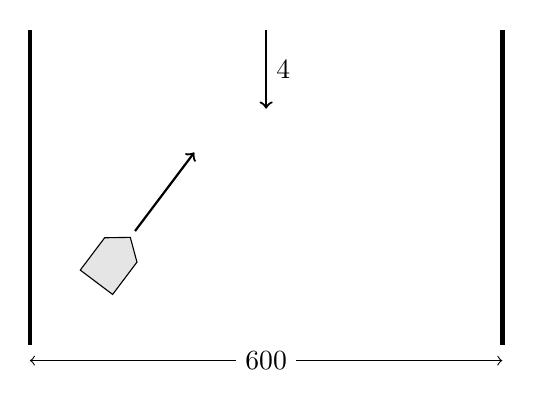
\begin{tikzpicture}
        %% Banks
        \draw[ultra thick] (-3,-2) -- (-3,2);
        \draw[ultra thick] (+3,-2) -- (+3,2);
        \draw[<->] (-3,-2.2) -- (+3,-2.2) node[pos=0.5,anchor=center,fill=white] {\SI{600}{\meter}};
        %% Boat
        \node[rotate=53,minimum size=0.5cm] (B) at (-2,-1) {};
        \draw[fill=white!90!black] (B.east) ++ (53:0.20) -- (B.south east) -- (B.south west) -- (B.north west) -- (B.north east) --cycle;
        \draw[thick,->] (B.east) ++(53:0.3) -- ++(53:1.25);
        %% Current
        \draw[thick,->] (0,+2) -- (0,+1) node[pos=0.5,anchor=west] {\SI{4}{\meter\per\second}};
    \end{tikzpicture}
    \end{center}
    The time it takes to cross the river is closest to:
    \begin{multicols}{3}
    \begin{choices}
        \wrongchoice{\SI{67}{\second}}
        \wrongchoice{\SI{120}{\second}}
        \wrongchoice{\SI{150}{\second}}
      \correctchoice{\SI{200}{\second}}
        \wrongchoice{\SI{600}{\second}}
    \end{choices}
    \end{multicols}
\end{question}
}

\element{aapt}{ %% Olympiad-A1
\begin{question}{olympiad-2015-q02}
    A car travels directly north on a straight highway at a constant speed of \SI{80}{\kilo\meter\per\hour} for a distance of \SI{25}{\kilo\meter}.
    The car then continues directly north at a constant speed of \SI{50}{\kilo\meter\per\hour} for a distance of \SI{75}{\kilo\meter}.
    The average speed of the car for the entire journey is closest to:
    \begin{multicols}{2}
    \begin{choices}
      \correctchoice{\SI{55.2}{\kilo\meter\per\hour}}
        \wrongchoice{\SI{57.5}{\kilo\meter\per\hour}}
        \wrongchoice{\SI{65}{\kilo\meter\per\hour}}
        \wrongchoice{\SI{69.6}{\kilo\meter\per\hour}}
        \wrongchoice{\SI{72.5}{\kilo\meter\per\hour}}
    \end{choices}
    \end{multicols}
\end{question}
}

\element{aapt}{ %% Olympiad-A4
\begin{question}{olympiad-2015-q03}
    The force of friction on an airplane in level flight is given by $F_f = kv^2$,
        where $k$ is some constant, and $v$ is the speed of the airplane.
    When the power output from the engines is $P_0$,
        the plane is able to fly at a speed $v_0$.
    If the power output of the engines is increased by \SI{100}{\percent} to $2P_0$,
        the airplane will be able to fly at a new speed given by:
    \begin{multicols}{3}
    \begin{choices}
        \wrongchoice{$1.12 v_0$}
      \correctchoice{$1.26 v_0$}
        \wrongchoice{$1.41 v_0$}
        \wrongchoice{$2.82 v_0$}
        \wrongchoice{$8 v_0$}
    \end{choices}
    \end{multicols}
\end{question}
}

\element{aapt}{ %% Olympiad-A3
\begin{question}{olympiad-2015-q04}
    A \SI{2.0}{\kilo\gram} box is originally at rest on a horizontal surface
        where the coefficient of static friction between the box and the surface
        is $\mu_s$ and the coefficient of the kinetic friction between the box
        and the surface is $\mu_k=\num{0.90}\mu_s$.
    An external horizontal force of magnitude $P$ is then applied to the box.
    Which of the following is a graph of the acceleration of the box a versus the external force $P$?
    \begin{multicols}{2}
    \begin{choices}
        \AMCboxDimensions{down=-2.5em}
        %% ANS is A
        \correctchoice{
            \begin{tikzpicture}
                \begin{axis}[
                    axis y line=left,
                    axis x line=bottom,
                    axis line style={->},
                    xlabel={Force $P$},
                    xtick=\empty,
                    ylabel={acceleration $a$},
                    ytick=\empty,
                    xmin=0,xmax=11,
                    ymin=0,ymax=11,
                    width=0.95\columnwidth,
                    very thin,
                ]
                \addplot[line width=1pt,mark=\empty] plot coordinates {(0,0) (3,0) (3,1) (10,8)};
                \end{axis}
            \end{tikzpicture}
        }
        \wrongchoice{
            \begin{tikzpicture}
                \begin{axis}[
                    axis y line=left,
                    axis x line=bottom,
                    axis line style={->},
                    xlabel={Force $P$},
                    xtick=\empty,
                    ylabel={acceleration $a$},
                    ytick=\empty,
                    xmin=0,xmax=11,
                    ymin=0,ymax=11,
                    width=0.95\columnwidth,
                    very thin,
                ]
                \addplot[line width=1pt,mark=\empty] plot coordinates {(0,0) (3,0) (3,3) (10,10)};
                \end{axis}
            \end{tikzpicture}
        }
        \wrongchoice{
            \begin{tikzpicture}
                \begin{axis}[
                    axis y line=left,
                    axis x line=bottom,
                    axis line style={->},
                    xlabel={Force $P$},
                    xtick=\empty,
                    ylabel={acceleration $a$},
                    ytick=\empty,
                    xmin=0,xmax=11,
                    ymin=0,ymax=11,
                    width=0.95\columnwidth,
                    very thin,
                ]
                \addplot[line width=1pt,mark=\empty] plot coordinates {(0,0) (3,0) (10,7)};
                \end{axis}
            \end{tikzpicture}
        }
        \wrongchoice{
            \begin{tikzpicture}
                \begin{axis}[
                    axis y line=left,
                    axis x line=bottom,
                    axis line style={->},
                    xlabel={Force $P$},
                    xtick=\empty,
                    ylabel={acceleration $a$},
                    ytick=\empty,
                    xmin=0,xmax=11,
                    ymin=0,ymax=11,
                    width=0.95\columnwidth,
                    very thin,
                ]
                \addplot[line width=1pt,mark=\empty] plot coordinates {(0,3) (1,3) (8,11)};
                \end{axis}
            \end{tikzpicture}
        }
        \wrongchoice{
            \begin{tikzpicture}
                \begin{axis}[
                    axis y line=left,
                    axis x line=bottom,
                    axis line style={->},
                    xlabel={Force $P$},
                    xtick=\empty,
                    ylabel={acceleration $a$},
                    ytick=\empty,
                    xmin=0,xmax=11,
                    ymin=0,ymax=11,
                    width=0.95\columnwidth,
                    very thin,
                ]
                \addplot[line width=1pt,mark=\empty] plot coordinates {(0,0) (3,3) (3,4) (9,10)};
                \end{axis}
            \end{tikzpicture}
        }
    \end{choices}
    \end{multicols}
\end{question}
}

\element{aapt}{
\begin{question}{olympiad-2015-q05}
    A \SI{470}{\gram} lead ball is launched at a 60 degree angle above the horizontal with an initial speed of \SI{100}{\meter\per\second} directly toward a target on a vertical cliff wall that is \SI{150}{\meter} away as shown in the figure.
    \begin{center}
    \begin{tikzpicture}
        %% NOTE: TODO: tikz draw
        \draw (-5,0) -- (0,0)  -- (0,2.88);
        \draw (-5,0) -- ++(60:5);
    \end{tikzpicture}
    \end{center}
    Ignoring air friction,
        by what distance does the lead ball miss the target when it hits the cliff wall?
    \begin{multicols}{3}
    \begin{choices}
        \wrongchoice{\SI{1.3}{\meter}}
        \wrongchoice{\SI{2.2}{\meter}}
        \wrongchoice{\SI{5.0}{\meter}}
        \wrongchoice{\SI{7.1}{\meter}}
      \correctchoice{\SI{11}{\meter}}
    \end{choices}
    \end{multicols}
\end{question}
}

\element{aapt}{ %% Olympiad-A5
\begin{question}{olympiad-2015-q06}
    Three trolley carts are free to move on a one dimensional frictionless horizontal track.
    Cart $A$ has a mass of \SI{1.9}{\kilo\gram} and an initial speed of \SI{1.7}{\meter\per\second} to the right;
    Cart $B$ has a mass of \SI{1.1}{\kilo\gram} and an initial speed of \SI{2.5}{\meter\per\second} to the left;
    Cart $C$ has a mass of \SI{1.3}{\kilo\gram} and is originally at rest.
    Collisions between carts $A$ and $B$ are perfectly elastic;
        collisions between carts $B$ and $C$ are perfectly inelastic.
    \begin{center}
    \begin{tikzpicture}
        %% Ground
        \draw[ultra thick] (-4,0) -- (4,0);
        %% Cars
        \node[draw,minimum width=1cm,minimum height=1.5em,anchor=south] (A) at (-3,0.2) {\SI{1.9}{\kilo\gram}};
        \node[draw,minimum width=1cm,minimum height=1.5em,anchor=south] (B) at  (0,0.2) {\SI{1.1}{\kilo\gram}};
        \node[draw,minimum width=1cm,minimum height=1.5em,anchor=south] (C) at (+3,0.2) {\SI{1.3}{\kilo\gram}};
        %% Wheels
        \draw (A.south east) ++(-0.15,-0.1) circle (0.1);
        \draw (A.south west) ++(+0.15,-0.1) circle (0.1);
        \draw (B.south east) ++(-0.15,-0.1) circle (0.1);
        \draw (B.south west) ++(+0.15,-0.1) circle (0.1);
        \draw (C.south east) ++(-0.15,-0.1) circle (0.1);
        \draw (C.south west) ++(+0.15,-0.1) circle (0.1);
        %% Labels
        \node[anchor=south] at (A.north) {Cart $A$};
        \node[anchor=south] at (B.north) {Cart $B$};
        \node[anchor=south] at (C.north) {Cart $C$};
        %% Velocity
        \draw[thick,->] (-3.5,-0.5) -- (-2.5,-0.5) node[pos=0.5,anchor=north] {\SI{1.7}{\meter\per\second}};
        \draw[thick,->] (+0.5,-0.5) -- (-0.5,-0.5) node[pos=0.5,anchor=north] {\SI{2.5}{\meter\per\second}};
    \end{tikzpicture}
    \end{center}
    What is the velocity of the center of mass of the system of the three carts after the last collision?
    \begin{multicols}{3}
    \begin{choices}
      \correctchoice{\SI{0.11}{\meter\per\second}}
        \wrongchoice{\SI{0.16}{\meter\per\second}}
        \wrongchoice{\SI{1.4}{\meter\per\second}}
        \wrongchoice{\SI{2.0}{\meter\per\second}}
        \wrongchoice{\SI{3.23}{\meter\per\second}}
    \end{choices}
    \end{multicols}
\end{question}
}

\newcommand{\OlympiadTwentyFifteenQSeven}{
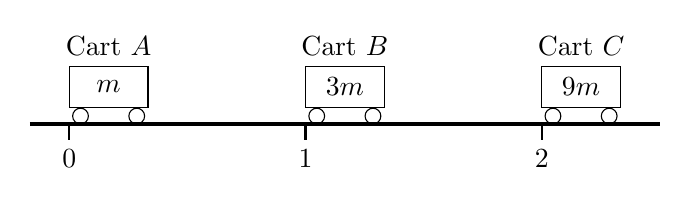
\begin{tikzpicture}
    %% Ground
    \draw[ultra thick] (-4,0) -- (4,0);
    %% Cars
    \node[draw,minimum width=1cm,minimum height=1.5em,anchor=south] (A) at (-3,0.2) {$m$};
    \node[draw,minimum width=1cm,minimum height=1.5em,anchor=south] (B) at  (0,0.2) {$3m$};
    \node[draw,minimum width=1cm,minimum height=1.5em,anchor=south] (C) at (+3,0.2) {$9m$};
    %% Wheels
    \draw (A.south east) ++(-0.15,-0.1) circle (0.1);
    \draw (A.south west) ++(+0.15,-0.1) circle (0.1);
    \draw (B.south east) ++(-0.15,-0.1) circle (0.1);
    \draw (B.south west) ++(+0.15,-0.1) circle (0.1);
    \draw (C.south east) ++(-0.15,-0.1) circle (0.1);
    \draw (C.south west) ++(+0.15,-0.1) circle (0.1);
    %% Labels
    \node[anchor=south] at (A.north) {Cart $A$};
    \node[anchor=south] at (B.north) {Cart $B$};
    \node[anchor=south] at (C.north) {Cart $C$};
    %% Markers
    \draw[thick] (-3.5,0) -- (-3.5,-0.2) node[anchor=north] {\SI{0}{\meter}};
    \draw[thick] (-0.5,0) -- (-0.5,-0.2) node[anchor=north] {\SI{1}{\meter}};
    \draw[thick] (+2.5,0) -- (+2.5,-0.2) node[anchor=north] {\SI{2}{\meter}};
\end{tikzpicture}
}

\element{aapt}{ %% Olympiad-A5
\begin{question}{olympiad-2015-q07}
    %% The following information applies to questions 7 and 8
    Carts $A$, $B$, and $C$ are on a long horizontal frictionless track.
    The masses of the carts are $m$, $3m$, and $9m$.
    Originally cart $B$ is at rest at the \SI{1.0}{\meter} mark and cart $C$ is at rest on the \SI{2.0}{\meter} mark.
    Cart $A$ is originally at the zero meter mark moving toward the cart $B$ at a speed of $v_0$.
    \begin{center}
        \OlympiadTwentyFifteenQSeven
    \end{center}
    Assuming that all collisions are completely inelastic,
        what is the final speed of cart $C$?
    \begin{multicols}{3}
    \begin{choices}
      \correctchoice{$\dfrac{1}{13} v_0$}
        \wrongchoice{$\dfrac{1}{10} v_0$}
        \wrongchoice{$\dfrac{1}{9} v_0$}
        \wrongchoice{$\dfrac{1}{3} v_0$}
        \wrongchoice{$\dfrac{2}{5} v_0$}
    \end{choices}
    \end{multicols}
\end{question}
}

\element{aapt}{ %% Olympiad-A5
\begin{question}{olympiad-2015-q08}
    %% The following information applies to questions 7 and 8
    Carts $A$, $B$, and $C$ are on a long horizontal frictionless track.
    The masses of the carts are $m$, $3m$, and $9m$.
    Originally cart $B$ is at rest at the \SI{1.0}{\meter} mark and cart $C$ is at rest on the \SI{2.0}{\meter} mark.
    Cart $A$ is originally at the zero meter mark moving toward the cart $B$ at a speed of $v_0$.
    \begin{center}
        \OlympiadTwentyFifteenQSeven
    \end{center}
    Assuming that all collisions are completely elastic,
        what is the final speed of cart $C$?
    \begin{multicols}{3}
    \begin{choices}
        \wrongchoice{$\dfrac{1}{8} v_0$}
      \correctchoice{$\dfrac{1}{4} v_0$}
        \wrongchoice{$\dfrac{1}{2} v_0$}
        \wrongchoice{$ v_0$}
        \wrongchoice{$2 v_0$}
    \end{choices}
    \end{multicols}
\end{question}
}

\element{aapt}{ %% Olympiad-A5
\begin{question}{olympiad-2015-q09}
    %The following information applies to questions 9 and 10
    A \SI{0.650}{\kilo\gram} ball moving at \SI{5.00}{\meter\per\second} collides with a \SI{0.750}{\kilo\gram} ball that is originally at rest.
    After the collision,
        the \SI{0.750}{\kilo\gram} ball moves off with a speed of \SI{4.00}{\meter\per\second},
        and the \SI{0.650}{\kilo\gram} ball moves off at a right angle to the final direction of motion of the \SI{0.750}{\kilo\gram} ball.
    %% Start question
    What is the final speed of the \SI{0.650}{\kilo\gram} ball?
    \begin{multicols}{2}
    \begin{choices}
      \correctchoice{\SI{1.92}{\meter\per\second}}
        \wrongchoice{\SI{2.32}{\meter\per\second}}
        \wrongchoice{\SI{3.00}{\meter\per\second}}
        \wrongchoice{\SI{4.64}{\meter\per\second}}
        \wrongchoice{\SI{5.77}{\meter\per\second}}
    \end{choices}
    \end{multicols}
\end{question}
}

\element{aapt}{ %% Olympiad-A5
\begin{question}{olympiad-2015-q10}
    %The following information applies to questions 9 and 10
    A \SI{0.650}{\kilo\gram} ball moving at \SI{5.00}{\meter\per\second} collides with a \SI{0.750}{\kilo\gram} ball that is originally at rest.
    After the collision,
        the \SI{0.750}{\kilo\gram} ball moves off with a speed of \SI{4.00}{\meter\per\second},
        and the \SI{0.650}{\kilo\gram} ball moves off at a right angle to the final direction of motion of the \SI{0.750}{\kilo\gram} ball.
    %% Start question
    Let the change in total kinetic energy in this collision be defined by $\Delta K=K_f - K_i$,
        where $K_f$ is the total final kinetic energy,
        and $K_i$ is the total initial kinetic energy.
    Which of the following is true?
    \begin{multicols}{2}
    \begin{choices}
        \wrongchoice{$\Delta K = \dfrac{K_i+K_f}{2}$}
        \wrongchoice{$K_f < \Delta K < K_i$}
        \wrongchoice{$0 < \Delta K < K_f$}
        \wrongchoice{$\Delta K = 0$}
      \correctchoice{$-K_i < \Delta K < 0$}
    \end{choices}
    \end{multicols}
\end{question}
}

\element{aapt}{
\begin{question}{olympiad-2015-q11}
    A sphere floats in water with $2/3$ of the volume of the sphere submerged.
    The sphere is removed and placed in oil that has $3/4$ the density of water.
    If it floats in the oil,
        what fraction of the sphere would be submerged in the oil?
    \begin{multicols}{2}
    \begin{choices}
        \wrongchoice{$\dfrac{1}{12}$}
        \wrongchoice{$\dfrac{1}{2}$}
      \correctchoice{$\dfrac{8}{9}$}
        \wrongchoice{$\dfrac{17}{12}$}
        \wrongchoice{The sphere will not float, it will sink in the oil.}
    \end{choices}
    \end{multicols}
\end{question}
}

\element{aapt}{ %% Olympiad-A8
\begin{question}{olympiad-2015-q12}
    %%The following information applies to questions 12 and 13
    A pendulum consists of a small bob of mass $m$ attached to a fixed point by a string of length $L$.
    The pendulum bob swings down from rest from an initial angle $\theta_{max} < \ang{90}$.
    %% Begin Question
    Which of the following statements about the pendulum bob's acceleration is true?
    \begin{choices}
        \wrongchoice{The magnitude of the acceleration is constant for the motion.}
        \wrongchoice{The magnitude of the acceleration at the lowest point is $g$, the acceleration of free fall.}
        \wrongchoice{The magnitude of the acceleration is zero at some point of the pendulum’s swing.}
        \wrongchoice{The acceleration is always directed toward the center of the circle.}
      \correctchoice{The acceleration at the bottom of the swing is pointing vertically upward.}
    \end{choices}
\end{question}
}

\element{aapt}{ %% Olympiad-A8
\begin{question}{olympiad-2015-q13}
    %%The following information applies to questions 12 and 13
    A pendulum consists of a small bob of mass $m$ attached to a fixed point by a string of length $L$.
    The pendulum bob swings down from rest from an initial angle $\theta_{max}<\ang{90}$.
    %% Begin Question
    Consider the pendulum bob when it is at an angle $\theta=\dfrac{1}{2}\theta_{max}$ on the way up (moving toward $\theta_{max}$).
    What is the direction of the acceleration vector?
    \begin{multicols}{2}
    \begin{choices}
        \AMCboxDimensions{down=-1.5cm}
        \wrongchoice{
            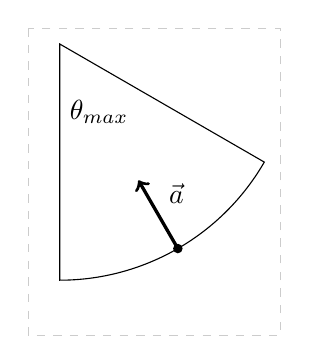
\begin{tikzpicture}
                \draw[dashed,white!80!black] (-0.4,0.2) rectangle (2.8,-3.7);
                \draw (0,0) -- (0,-3) arc (270:330:3) -- cycle;
                \draw[fill] (300:3) circle (1.5pt);
                \node[anchor=center] at (300:1) {$\theta_{max}$};
                \draw[very thick,->] (300:3)  -- ++(120:1) node[pos=0.5,anchor=south west] {$\vec{a}$};
            \end{tikzpicture}
        }
        \wrongchoice{
            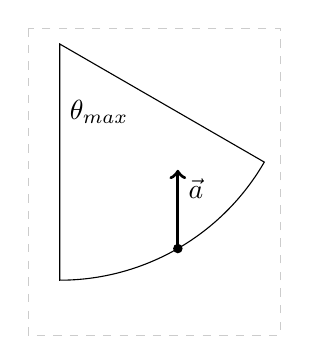
\begin{tikzpicture}
                \draw[dashed,white!80!black] (-0.4,0.2) rectangle (2.8,-3.7);
                \draw (0,0) -- (0,-3) arc (270:330:3) -- cycle;
                \draw[fill] (300:3) circle (1.5pt);
                \node[anchor=center] at (300:1) {$\theta_{max}$};
                \draw[very thick,->] (300:3)  -- ++(90:1) node[pos=0.5,anchor=south west] {$\vec{a}$};
            \end{tikzpicture}
        }
        \wrongchoice{
            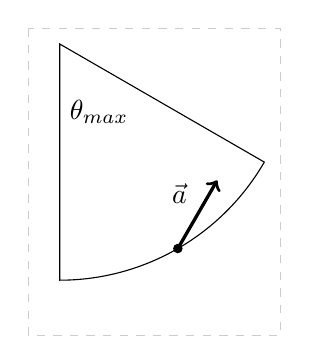
\begin{tikzpicture}
                \draw[dashed,white!80!black] (-0.4,0.2) rectangle (2.8,-3.7);
                \draw (0,0) -- (0,-3) arc (270:330:3) -- cycle;
                \draw[fill] (300:3) circle (1.5pt);
                \node[anchor=center] at (300:1) {$\theta_{max}$};
                \draw[very thick,->] (300:3)  -- ++(60:1) node[pos=0.5,anchor=south east] {$\vec{a}$};
            \end{tikzpicture}
        }
        %% ANS is D: angle is 135 if \theta=60, \theta/2=30
        %% changed to 160 to avoid confusion with A
        \correctchoice{
            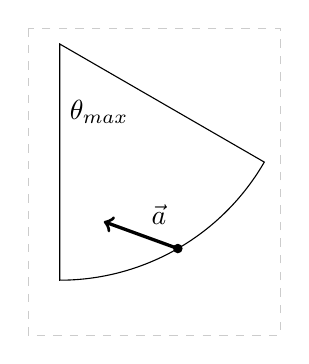
\begin{tikzpicture}
                \draw[dashed,white!80!black] (-0.4,0.2) rectangle (2.8,-3.7);
                \draw (0,0) -- (0,-3) arc (270:330:3) -- cycle;
                \draw[fill] (300:3) circle (1.5pt);
                \node[anchor=center] at (300:1) {$\theta_{max}$};
                \draw[very thick,->] (300:3)  -- ++(160:1) node[pos=0.5,anchor=south west] {$\vec{a}$};
            \end{tikzpicture}
        }
        \wrongchoice{
            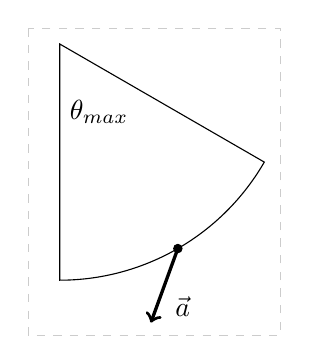
\begin{tikzpicture}
                \draw[dashed,white!80!black] (-0.4,0.2) rectangle (2.8,-3.7);
                \draw (0,0) -- (0,-3) arc (270:330:3) -- cycle;
                \draw[fill] (300:3) circle (1.5pt);
                \node[anchor=center] at (300:1) {$\theta_{max}$};
                \draw[very thick,->] (300:3)  -- ++(250:1) node[pos=0.5,anchor=north west] {$\vec{a}$};
            \end{tikzpicture}
        }
    \end{choices}
    \end{multicols}
\end{question}
}

\element{aapt}{ %% Olympiad-A6
\begin{question}{olympiad-2015-q14}
    %%The following information applies to questions 14 and 15
    A \SI{3.0}{\meter} long massless rod is free to rotate horizontally about its center.
    Two \SI{5.0}{\kilo\gram} point objects are originally located at the ends of the rod;
        they are free to slide on the frictionless rod and are kept from flying off the rod by an inflexible massless rope that connects the two objects.
    Originally the system is rotating at \SI{4.0}{\radian\per\second};
        assume the system is completely frictionless;
        and ignore any concerns about instability of the system.
    %% Begin Question
    Calculate the original tension in the rope.
    \begin{multicols}{3}
    \begin{choices}
        \wrongchoice{\SI{60}{\newton}}
        \wrongchoice{\SI{106}{\newton}}
      \correctchoice{\SI{120}{\newton}}
        \wrongchoice{\SI{240}{\newton}}
        \wrongchoice{\SI{480}{\newton}}
    \end{choices}
    \end{multicols}
\end{question}
}

\element{aapt}{ %% Olympiad-A6
\begin{question}{olympiad-2015-q15}
    %%The following information applies to questions 14 and 15
    A \SI{3.0}{\meter} long massless rod is free to rotate horizontally about its center.
    Two \SI{5.0}{\kilo\gram} point objects are originally located at the ends of the rod;
        they are free to slide on the frictionless rod and are kept from flying off the rod by an inflexible massless rope that connects the two objects.
    Originally the system is rotating at \SI{4.0}{\radian\per\second};
        assume the system is completely frictionless;
        and ignore any concerns about instability of the system.
    %% Begin Question
    The rope is slowly tightened by a small massless motor attached to one of the objects.
    It is done in such a way as to pull the two objects closer to the center of the rotating rod.
    How much work is done by the motor in pulling the two objects from the ends of the rod until they are each \SI{0.5}{\meter} from the center of rotation?
    \begin{multicols}{3}
    \begin{choices}
        \wrongchoice{\SI{120}{\joule}}
        \wrongchoice{\SI{180}{\joule}}
        \wrongchoice{\SI{240}{\joule}}
      \correctchoice{\SI{1440}{\joule}}
        \wrongchoice{\SI{1620}{\joule}}
    \end{choices}
    \end{multicols}
\end{question}
}

\element{aapt}{
\begin{question}{olympiad-2015-q16}
    Shown below is a graph of potential energy as a function of position for a \SI{0.50}{\kilo\gram} object.
    \begin{center}
    \begin{tikzpicture}
        %% NOTE: how to draw?
        \begin{axis}[
            axis y line=left,
            axis x line=middle,
            axis line style={->},
            xlabel={position},
            x unit=\si{\centi\meter},
            xtick={0,1,2,3,4,5,6},
            minor x tick num=1,
            ylabel={energy},
            y unit=\si{\joule},
            ytick={-10,0,10,20},
            minor x tick num=1,
            grid=major,
            xmin=0,xmax=6.1,
            ymin=-12,ymax=22,
            width=0.8\columnwidth,
            height=0.5\columnwidth,
        ]
        %% NOTE: TODO: add function
        %\addplot[line width=1pt,smooth,domain=0:6] plot coordinates {x};
        \addplot[line width=1pt,smooth,domain=0:6] {x};
        \end{axis}
    \end{tikzpicture}
    \end{center}
    Which of the following statements is \emph{not} true in the range $\SI{0}{\centi\meter} < x < \SI{6}{\centi\meter}$?
    \begin{choices}
        \wrongchoice{The object could be at equilibrium at either $x=\SI{1}{\centi\meter}$ or $x=\SI{3}{\centi\meter}$.}
        \wrongchoice{The minimum possible total energy for this object in the range is \SI{-10}{\joule}.}
        \wrongchoice{The magnitude of the force on the object at \SI{4}{\centi\meter} is approximately \SI{1000}{\newton}.}
        \wrongchoice{If the total energy of the particle is \SI{0}{\joule} then the object will have a maximum kinetic energy of \SI{10}{\joule}.}
      \correctchoice{The magnitude of the acceleration of the object at $x=\SI{2}{\centi\meter}$ is approximately \SI{4}{\centi\meter\per\second\squared}.}
    \end{choices}
\end{question}
}

\element{aapt}{ %% Olympiad-A6
\begin{question}{olympiad-2015-q17}
    A flywheel can rotate in order to store kinetic energy.
    The flywheel is a uniform disk made of a material with a density $\rho$ and tensile strength $\sigma$ (measured in Pascals---\si{\pascal}),
        a radius $r$, and a thickness $h$.
    The flywheel is rotating at the maximum possible angular velocity so that it does not break.
    Which of the following expression correctly gives the maximum kinetic energy per kilogram that can be stored in the flywheel?
    Assume that $\alpha$ is a dimensionless constant.
    \begin{multicols}{2}
    \begin{choices}
        \wrongchoice{$\alpha \sqrt{\dfrac{\rho \sigma}{4}}$}
        \wrongchoice{$\alpha h\sqrt{\dfrac{\rho\sigma}{r}}$}
        \wrongchoice{$\alpha \sqrt{\dfrac{h}{r}}\left(\dfrac{\sigma}{\rho}\right)^2$}
        \wrongchoice{$\alpha \left(\dfrac{h}{r}\right)\left(\dfrac{\sigma}{\rho}\right)$}
      \correctchoice{$\dfrac{\alpha\sigma}{\rho}$}
    \end{choices}
    \end{multicols}
\end{question}
}

\element{aapt}{
\begin{question}{olympiad-2015-q18}
    Shown below are three graphs of the same data.
    \begin{center}
    \begin{tikzpicture}
        %% NOTE: TODO: check functions and add marks
        \begin{groupplot}[
                group style={group size=1 by 3},
                axis y line=left,
                axis x line=bottom,
                axis line style={->},
                width=0.8\columnwidth,
                height=0.5\columnwidth,
                xtick=\empty,
                ytick=\empty,
            ]
            \nextgroupplot[
                xlabel={$y$},
                ylabel={$x$},
                xmin=0,xmax=10,
                ymin=0,ymax=10,
            ] \addplot[domain=0:10] {1*exp(0.2*x)};
            \nextgroupplot[
                xlabel={$x$},
                ylabel={$\log\left(y\right)$},
                xmin=0,xmax=10,
                ymin=0,ymax=10,
            ] \addplot[domain=0:10] {1+x};
            \nextgroupplot[
                xlabel={$\log\left(x\right)$},
                ylabel={$\log\left(y\right)$},
                xmin=0,xmax=10,
                ymin=0,ymax=10,
            ] \addplot[domain=0:10] {1 + ln(x)};
        \end{groupplot}
    \end{tikzpicture}
    \end{center}
    Which is the correct functional relationship between the data points?
    Assume $a$ and $b$ are constants.
    \begin{multicols}{2}
    \begin{choices}
        \wrongchoice{$y = ax + b$}
        \wrongchoice{$y = ax^2 + b$}
        \wrongchoice{$y = ax^b$}
      \correctchoice{$y = a\mathrm{e}^{bx}$}
        \wrongchoice{$y = a\log x + b$}
    \end{choices}
    \end{multicols}
\end{question}
}

\element{aapt}{
\begin{question}{olympiad-2015-q19}
    %%The following information applies to questions 19 and 20
    A U-tube manometer consists of a uniform diameter cylindrical tube that is bent into a U shape.
    It is originally filled with water that has a density $\rho_w$.
    The total length of the column of water is $L$.
    Ignore surface tension and viscosity.
    \begin{center}
    \begin{tikzpicture}
        %% NOTE: TODO: include diagram to help scaffold!
    \end{tikzpicture}
    \end{center}
    %% Begin Question
    The water is displaced slightly so that one side moves up a distance $x$ and the other side lowers a distance $x$.
    Find the frequency of oscillation.
    \begin{multicols}{2}
    \begin{choices}
      \correctchoice{$\dfrac{1}{2\pi} \sqrt{\dfrac{2g}{L}}$}
        \wrongchoice{$2\pi \sqrt{\dfrac{g}{L}}$}
        \wrongchoice{$\dfrac{1}{2\pi} \sqrt{\dfrac{2L}{g}}$}
        \wrongchoice{$\dfrac{1}{2\pi} \sqrt{\dfrac{g}{\rho_W}}$}
        \wrongchoice{$2\pi \sqrt{\rho_W gL}$}
    \end{choices}
    \end{multicols}
\end{question}
}

\element{aapt}{
\begin{question}{olympiad-2015-q20}
    Oil with a density half that of water is added to one side of the tube until the total length of oil is equal to the total length of water.
    Determine the equilibrium height difference between the two sides:
    \begin{multicols}{3}
    \begin{choices}
        \wrongchoice{$L$}
      \correctchoice{$\dfrac{L}{2}$}
        \wrongchoice{$\dfrac{L}{3}$}
        \wrongchoice{$\dfrac{3L}{4}$}
        \wrongchoice{$\dfrac{L}{4}$}
    \end{choices}
    \end{multicols}
\end{question}
}

\element{aapt}{ %% Olympiad-A2
\begin{question}{olympiad-2015-q21}
    An object launched vertically upward from the ground with a speed of \SI{50}{\meter\per\second} bounces off of the ground on the return trip with a coefficient of restitution given by $C_R=0.9$,
        meaning that immediately after a bounce the upward speed is \SI{90}{\percent} of the previous downward speed.
    The ball continues to bounce like this;
        what is the total amount of time between when the ball is launched and when it finally comes to a rest?
    Assume the collision time is zero; the bounce is instantaneous.
    Treat the problem as ideally classical and ignore any quantum effects that might happen for very small bounces.
    \begin{multicols}{2}
    \begin{choices}
        \wrongchoice{\SI{71}{\second}}
      \correctchoice{\SI{100}{\second}}
        \wrongchoice{\SI{141}{\second}}
        \wrongchoice{\SI{1000}{\second}}
        \wrongchoice{$\infty$ (the ball never comes to a rest)}
    \end{choices}
    \end{multicols}
\end{question}
}

\element{aapt}{
\begin{question}{olympiad-2015-q22}
    A solid ball is released from rest down inclines of various inclination angles $\theta$ but through a fixed vertical height $h$.
    The coefficient of static and kinetic friction are both equal to $\mu$.
    Which of the following graphs best represents the total kinetic energy of the ball at the bottom of the incline as a function of the angle of the incline?
    \begin{multicols}{2}
    \begin{choices}
        %% ANS is C
        \wrongchoice{
            \begin{tikzpicture}
                %% NOTE:
            \end{tikzpicture}
        }
    \end{choices}
    \end{multicols}
\end{question}
}

\element{aapt}{ %% Olympiad-A5
\begin{question}{olympiad-2015-q23}
    A \SI{2.0}{\kilo\gram} object falls from rest a distance of \SI{5.0}{\meter} onto a \SI{6.0}{\kilo\gram} object that is supported by a vertical massless spring with spring constant k = 72 N/m.
    The two objects stick together after the collision,
        which results in the mass/spring system oscillating.
    What is the maximum magnitude of the displacement of the \SI{6.0}{\kilo\gram} object from its original location before it is struck by the falling object?
    \begin{multicols}{3}
    \begin{choices}
        \wrongchoice{\SI{0.27}{\meter}}
      \correctchoice{\SI{1.1}{\meter}}
        \wrongchoice{\SI{2.5}{\meter}}
        \wrongchoice{\SI{2.8}{\meter}}
        \wrongchoice{\SI{3.1}{\meter}}
    \end{choices}
    \end{multicols}
\end{question}
}

\element{aapt}{ %% Olympiad-A8
\begin{question}{olympiad-2015-q24}
    The speed of a transverse wave on a long cylindrical steel string is given by:
    \begin{equation*}
        v = \sqrt{\dfrac{TL}{M}}\, ,
    \end{equation*}
    where $T$ is the tension in the string,
        $M$ is the mass, and $L$ is the length of the string.
    Ignore any string stiffness,
        and assume that it does not stretch when tightened.
    Consider two steel strings of the same length,
        the first with radius $r_1$ and a second thicker string with radius $r_2=4r_1$.
    Each string is tightened to the maximum possible tension without breaking.
    What is the ratio $\dfrac{f_1}{f_2}$ of the fundamental frequencies of vibration on the two strings?
    \begin{multicols}{3}
    \begin{choices}
      \correctchoice{$1$}
        \wrongchoice{$\sqrt{2}$}
        \wrongchoice{$2$}
        \wrongchoice{$2\sqrt{2}$}
        \wrongchoice{$4$}
    \end{choices}
    \end{multicols}
\end{question}
}

\element{aapt}{ %% Olympiad-A8
\begin{question}{olympiad-2015-q25}
    Two identical carts $A$ and $B$ each with mass $m$ are connected via a spring with spring constant $k$.
    Two additional springs, identical to the first,
        connect the carts to two fixed points.
    The carts are free to oscillate under the effect of the springs in one dimensional frictionless motion.
    \begin{center}
    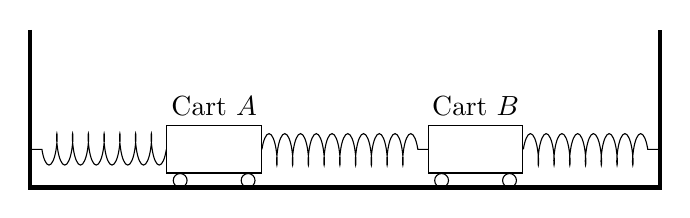
\begin{tikzpicture}
        \draw[ultra thick] (-4,2) -- (-4,0) -- (4,0) -- (4,2);
        %% Carts
        \node[draw,anchor=south,minimum width=1.2cm,minimum height=0.6cm] (A) at (-1.66,0.5em) {};
        \node[draw,anchor=south,minimum width=1.2cm,minimum height=0.6cm] (B) at (+1.66,0.5em) {};
        \node[anchor=south] at (A.north) {Cart $A$};
        \node[anchor=south] at (B.north) {Cart $B$};
        %% Wheels
        \draw (A.south west) ++(+0.5em,-0.25em) circle (0.25em);
        \draw (A.south east) ++(-0.5em,-0.25em) circle (0.25em);
        \draw (B.south west) ++(+0.5em,-0.25em) circle (0.25em);
        \draw (B.south east) ++(-0.5em,-0.25em) circle (0.25em);
        %% Spring
        \draw[decoration={aspect=0.2,segment length=2mm,amplitude=2mm,coil},decorate] (A.west) -- ++(180:1.75);
        \draw[decoration={aspect=0.2,segment length=2mm,amplitude=2mm,coil},decorate] (A.east) -- (B.west);
        \draw[decoration={aspect=0.2,segment length=2mm,amplitude=2mm,coil},decorate] (B.east) -- ++(0:1.75);
    \end{tikzpicture}
    \end{center}
    Under suitable initial conditions,
        the two carts will oscillate in phase according to
    \begin{equation*}
        x_A (t) = x_0 \sin\omega_1 t = x_B (t) \, ,
    \end{equation*}
    where $x_A$ and $x_B$ are the locations of carts $A$ and $B$ relative to their respective equilibrium positions.
    Under other suitable initial conditions,
        the two carts will oscillate exactly out of phase according to
    \begin{equation*}
        x_A (t) = x_0 \sin\omega_2 t = -x_B(t) \, ,
    \end{equation*}
    Determine the ratio $\dfrac{\omega_2}{\omega_1}$:
    \begin{multicols}{3}
    \begin{choices}
      \correctchoice{$\sqrt{3}$}
        \wrongchoice{$2$}
        \wrongchoice{$2\sqrt{2}$}
        \wrongchoice{$3$}
        \wrongchoice{$5$}
    \end{choices}
    \end{multicols}
\end{question}
}


%% PhysicsOlympiad 2014 F=ma Exam
%%----------------------------------------
\element{aapt}{ %% Olympiad-A6
\begin{question}{olympiad-2014-q01}
    A car turning to the right is traveling at constant speed in a circle.
    From the driver's perspective,
        the angular momentum vector about the center of the circle
        points $X$ and the acceleration vector of the car points $Y$ where
    \begin{choices}
        \wrongchoice{$X$ is left, $Y$ is left.}
        \wrongchoice{$X$ is forward, $Y$ is right.}
        \wrongchoice{$X$ is down, $Y$ is forward.}
        \wrongchoice{$X$ is left, $Y$ is right.}
      \correctchoice{$X$ is down, $Y$ is right.}
    \end{choices}
\end{question}
}

\element{aapt}{ %% Olympiad-A3
\begin{question}{olympiad-2014-q02}
    A ball rolls without slipping down an inclined plane as shown in the diagram.
    Which of the following vectors best represents the direction of the total
        force that the ball exerts on the plane?
    \begin{center}
    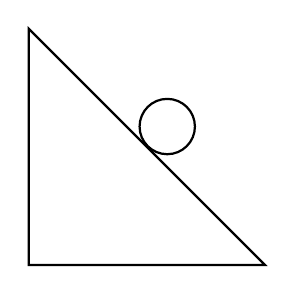
\begin{tikzpicture}
        \draw[thick] (0,0) -- (3,0) -- (0,3) -- cycle;
        \node[thick,draw,circle,minimum size=2em,anchor=south west] at (1.5,1.5) {};
    \end{tikzpicture}
    \end{center}
    \begin{multicols}{2}
    \begin{choices}
        \AMCboxDimensions{down=-0.85cm}
        \wrongchoice{
            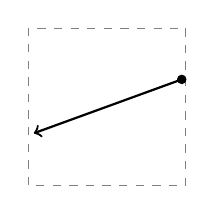
\begin{tikzpicture}
                \draw[dashed,draw=white!50!black] (+0.05,+0.65) rectangle (-1.95,-1.35);
                \draw[fill] (0,0) circle (1.5pt);
                \draw[thick,->] (0,0) -- (200:2.0cm);
            \end{tikzpicture}
        }
        \wrongchoice{
            \begin{tikzpicture}
                \draw[dashed,draw=white!50!black] (-2.00,-1.00) rectangle (0.0,+1.0);
                \draw[fill] (0,0) circle (1.5pt);
                \draw[thick,->] (0,0) -- (180:2.0cm);
            \end{tikzpicture}
        }
        \wrongchoice{
            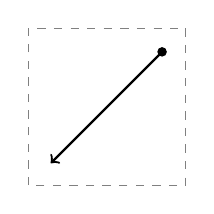
\begin{tikzpicture}
                \draw[dashed,draw=white!50!black] (+0.3,+0.3) rectangle (-1.7,-1.7);
                \draw[fill] (0,0) circle (1.5pt);
                \draw[thick,->] (0,0) -- (225:2.0cm);
            \end{tikzpicture}
        }
        \wrongchoice{
            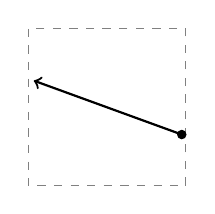
\begin{tikzpicture}
                \draw[dashed,draw=white!50!black] (+0.05,-0.65) rectangle (-1.95,+1.35);
                %\draw[dashed,draw=white!50!black] (-1.00,0.00) rectangle (+1.0,-2.0);
                \draw[fill] (0,0) circle (1.5pt);
                \draw[thick,->] (0,0) -- (160:2.0cm);
            \end{tikzpicture}
        }
        %% ANS is E
        %% The arrow is straight down in the case of 45 deg
        \correctchoice{
            \begin{tikzpicture}
                \draw[dashed,draw=white!50!black] (-1.00,-0.00) rectangle (+1.0,-2.0);
                \draw[fill] (0,0) circle (1.5pt);
                \draw[thick,->] (0,0) -- (270:2.0cm);
            \end{tikzpicture}
        }
    \end{choices}
    \end{multicols}
\end{question}
}

\element{aapt}{ %% aapt-F1
\begin{question}{olympiad-2014-q03}
    An object of uniform density floats partially submerged so that
        \SI{20}{\percent} of the object is above the water.
    A \SI{3}{\newton} force presses down on the top of the object
        so that the object becomes fully submerged.
    What is the volume of the object?
    The density of water is $\rho_{H_2O} = \SI{1000}{\kilo\gram\per\meter\cubed}$.
    \begin{multicols}{2}
    \begin{choices}
        \wrongchoice{$V_{object} = \SI{0.3}{\liter}$}
        \wrongchoice{$V_{object} = \SI{0.67}{\liter}$}
        \wrongchoice{$V_{object} = \SI{1.2}{\liter}$}
      \correctchoice{$V_{object} = \SI{1.5}{\liter}$}
        \wrongchoice{$V_{object} = \SI{3.0}{\liter}$}
    \end{choices}
    \end{multicols}
\end{question}
}

\element{aapt}{ %% Olympiad-A5
\begin{question}{olympiad-2014-q04}
    What are the correct values of the numbers in the following statements?
    Assume there are no external forces,
        and take $N = 1$ to mean that the statement cannot be made for any meaningful number of particles.
    \begin{itemize}
        \item If a particle at rest explodes into $N_1$ or fewer particles with known masses,
            and the total kinetic energy of the new particles is known,
            the kinetic energy of each of the new particles is completely determined.
        \item If a particle at rest explodes into $N_2$ or fewer particles,
            the velocities of the new particles must lie in a line.
        \item If a particle at rest explodes into $N_3$ or fewer particles,
            the velocities of the new particles must lie in a plane.
    \end{itemize}
    \begin{choices}
        \wrongchoice{$N_1 = 2$, $N_2 = 1$, $N_3 = 1$}
        \wrongchoice{$N_1 = 1$, $N_2 = 2$, $N_3 = 3$}
      \correctchoice{$N_1 = 2$, $N_2 = 2$, $N_3 = 3$}
        \wrongchoice{$N_1 = 3$, $N_2 = 2$, $N_3 = 3$}
        \wrongchoice{$N_1 = 2$, $N_2 = 3$, $N_3 = 4$}
    \end{choices}
\end{question}
}

\element{aapt}{ %% Olympiad-A6
\begin{question}{olympiad-2014-q05}
    A unicyclist goes around a circular track of radius \SI{30}{\meter}
        at a (\emph{amazingly fast}!) constant speed of \SI{10}{\meter\per\second}.
    At what angle to the left (or right) of vertical must the unicyclist lean to avoid falling?
    Assume that the height of the unicyclist is much smaller than the radius of the track.
    \begin{multicols}{3}
    \begin{choices}
        \wrongchoice{\ang{9.46}}
        \wrongchoice{\ang{9.59}}
      \correctchoice{\ang{18.4}}
        \wrongchoice{\ang{19.5}}
        \wrongchoice{\ang{70.5}}
    \end{choices}
    \end{multicols}
\end{question}
}

\element{aapt}{ %% Olympiad-A5
\begin{question}{olympiad-2014-q06}
    A cubical box of mass \SI{10}{\kilo\gram} with edge length
        \SI{5}{\meter} is free to move on a frictionless horizontal surface.
    Inside is a small block of mass \SI{2}{\kilo\gram},
        which moves without friction inside the box.
    At time $t=0$,
        the block is moving with velocity \SI{5}{\meter\per\second}
        directly towards one of the faces of the box,
        while the box is initially at rest.
    The coefficient of restitution for any collision between the block and box is \SI{90}{\percent},
        meaning that the relative speed between the box and block immediately after a collision is \SI{90}{\percent} of the relative speed between the box and block immediately before the collision.
    \begin{center}
    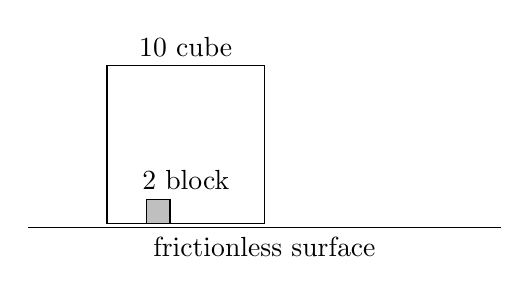
\begin{tikzpicture}
        %% Big box
        \draw (0,0) rectangle (2,2);
        \node[anchor=south] at (1,2) {\SI{10}{\kilo\gram} cube};
        %% small cube
        \draw[fill=white!75!black] (0.5,0) rectangle (0.8,0.3);
        \node[anchor=south] at (1.0,0.3) {\SI{2}{\kilo\gram} block};
        %% Frictionless surface
        \draw (-1,-0.05) -- (5,-0.05) node[pos=0.5,anchor=north] {frictionless surface};
    \end{tikzpicture}
    \end{center}
    After \SI{1}{\minute},
        the block is a displacement $x$ from the original position.
    Which of the following is closest to $x$?
    \begin{multicols}{3}
    \begin{choices}
        \wrongchoice{\SI{0}{\meter}}
      \correctchoice{\SI{50}{\meter}}
        \wrongchoice{\SI{100}{\meter}}
        \wrongchoice{\SI{200}{\meter}}
        \wrongchoice{\SI{300}{\meter}}
    \end{choices}
    \end{multicols}
\end{question}
}

\element{aapt}{ %% Olympiad-A6
\begin{question}{olympiad-2014-q07}
    A \SI{1.00}{\meter} long stick with uniform density is allowed
        to rotate about a point \SI{30.0}{\centi\meter} from its end.
    The stick is perfectly balanced when a \SI{50.0}{\gram}
        mass is placed on the stick \SI{20.0}{\centi\meter} from the same end.
    What is the mass of the stick?
    \begin{multicols}{3}
    \begin{choices}
        \wrongchoice{\SI{35.7}{\gram}}
        \wrongchoice{\SI{33.3}{\gram}}
      \correctchoice{\SI{25.0}{\gram}}
        \wrongchoice{\SI{17.5}{\gram}}
        \wrongchoice{\SI{14.3}{\gram}}
    \end{choices}
    \end{multicols}
\end{question}
}

\element{aapt}{ %% Olympiad-A8
\begin{question}{olympiad-2014-q08}
    An object of mass $M$ is hung on a vertical spring of spring constant $k$
        and is set into vertical oscillations.
    The period of this oscillation is $T_0$.
    The spring is then cut in half and the same mass is attached and the system
        is set up to oscillate on a frictionless inclined plane making an angle $\theta$
        to the horizontal.
    Determine the period of the oscillations on the inclined plane in terms of $T_0$.
    \begin{multicols}{3}
    \begin{choices}
        \wrongchoice{$T_0$}
        \wrongchoice{$\dfrac{T_0}{2}$}
        \wrongchoice{$2T_0\sin\theta$}
      \correctchoice{$\dfrac{T_0}{\sqrt{2}}$}
        \wrongchoice{$\dfrac{T_0\sin\theta}{\sqrt{2}}$}
    \end{choices}
    \end{multicols}
\end{question}
}

\element{aapt}{ %% Olympiad-A3
\begin{question}{olympiad-2014-q09}
    A \SI{5.0}{\kilo\gram} object undergoes a time-varying force as shown in the graph below.
    \begin{center}
    \begin{tikzpicture}
        \begin{axis}[
            axis y line=left,
            axis x line=bottom,
            axis line style={->},
            xlabel={time},
            x unit=\si{\second},
            xtick={0,1,2,3,4,5,6,7,8},
            minor x tick num=1,
            ylabel={force},
            y unit=\si{\newton},
            ytick={0,1,2,3,4},
            minor x tick num=1,
            grid=major,
            xmin=0,xmax=8.1,
            ymin=0,ymax=4.1,
            width=0.8\columnwidth,
            height=0.5\columnwidth,
        ]
        \addplot[line width=1pt,mark=\empty] plot coordinates { (0,0) (3,3) (7,1) (8,1) };
        \end{axis}
    \end{tikzpicture}
    \end{center}
    If the velocity at $t=\SI{0.0}{\second}$ is \SI[retain-explicit-plus]{+1.0}{\meter\per\second},
        what is the velocity of the object at $t=\SI{7}{\second}$?
    \begin{multicols}{2}
    \begin{choices}
        \wrongchoice{\SI{2.45}{\meter\per\second}}
        \wrongchoice{\SI{2.50}{\meter\per\second}}
      \correctchoice{\SI{3.50}{\meter\per\second}}
        \wrongchoice{\SI{12.5}{\meter\per\second}}
        \wrongchoice{\SI{15.0}{\meter\per\second}}
    \end{choices}
    \end{multicols}
\end{question}
}

\element{aapt}{ %% Olympiad-A6
\begin{question}{olympiad-2014-q10}
    A radio controlled car is attached to a stake in the ground by a \SI{3.00}{\meter}
        long piece of string, and is forced to move in a circular path.
    The car has an initial angular velocity of \SI{1.00}{\radian\per\second}
        and smoothly accelerates at a rate of \SI{4.00}{\radian\per\second\squared}.
    The string will break if the centripetal acceleration exceeds
        \SI{2.43e2}{\gram\per\second\squared}.
    How long can the car accelerate at this rate before the string breaks?
    \begin{multicols}{3}
    \begin{choices}
        \wrongchoice{\SI{0.25}{\second}}
        \wrongchoice{\SI{0.50}{\second}}
        \wrongchoice{\SI{1.00}{\second}}
        \wrongchoice{\SI{1.50}{\second}}
      \correctchoice{\SI{2.00}{\second}}
    \end{choices}
    \end{multicols}
\end{question}
}

\element{aapt}{ %% Olympiad-A4
\begin{question}{olympiad-2014-q11}
    A point mass $m$ is connected to an ideal spring on a horizontal frictionless surface.
    The mass is pulled a short distance and then released.
    Which of the following is the most correct plot of the kinetic energy
        as a function of potential energy?
    \begin{multicols}{2}
    \begin{choices}
        \AMCboxDimensions{down=-1.00cm}
        \wrongchoice{
            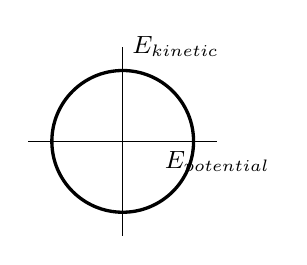
\begin{tikzpicture}[scale=0.60,font=\small]
                \draw (-2,0) -- (+2,0) node[anchor=north] {$E_{potential}$};
                \draw (0,-2) -- (0,+2) node[anchor=west] {$E_{kinetic}$};
                \draw[very thick] (0,0) circle (1.5cm);
            \end{tikzpicture}
        }
        \wrongchoice{
            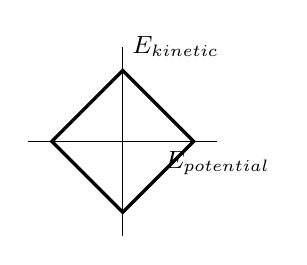
\begin{tikzpicture}[scale=0.60,font=\small]
                \draw (-2,0) -- (+2,0) node[anchor=north] {$E_{potential}$};
                \draw (0,-2) -- (0,+2) node[anchor=west] {$E_{kinetic}$};
                \draw[very thick] (-1.5,0) -- (0,1.5) -- (1.5,0) -- (0,-1.5) -- cycle;
            \end{tikzpicture}
        }
        \wrongchoice{
            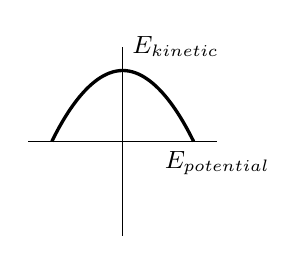
\begin{tikzpicture}[scale=0.60,font=\small]
                \draw (-2,0) -- (+2,0) node[anchor=north] {$E_{potential}$};
                \draw (0,-2) -- (0,+2) node[anchor=west] {$E_{kinetic}$};
                \draw[very thick] (-1.5,0) parabola bend (0,1.5) (1.5,0);
            \end{tikzpicture}
        }
        \wrongchoice{
            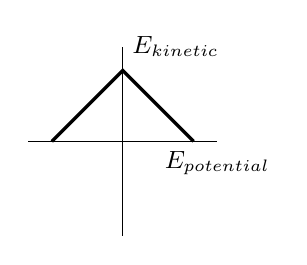
\begin{tikzpicture}[scale=0.60,font=\small]
                \draw (-2,0) -- (+2,0) node[anchor=north] {$E_{potential}$};
                \draw (0,-2) -- (0,+2) node[anchor=west] {$E_{kinetic}$};
                \draw[very thick] (-1.5,0) -- (0,1.5) -- (1.5,0);
            \end{tikzpicture}
        }
        %% ANS: E
        \correctchoice{
            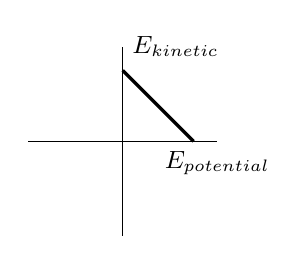
\begin{tikzpicture}[scale=0.60,font=\small]
                \draw (-2,0) -- (+2,0) node[anchor=north] {$E_{potential}$};
                \draw (0,-2) -- (0,+2) node[anchor=west] {$E_{kinetic}$};
                \draw[very thick] (0,1.5) -- (1.5,0);
            \end{tikzpicture}
        }
    \end{choices}
    \end{multicols}
\end{question}
}

\newcommand{\OlympiadTwentyFourteenQTwelve}{
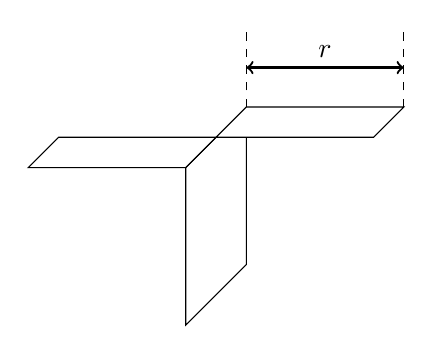
\begin{tikzpicture}
    %% Left wing
    \draw (0,0,0) -- (-2,0,0) -- (-2,0,-1) -- (0,0,-1) -- cycle;
    %% Main body
    \draw (0,0,0) -- (0,-2,0) -- (0,-2,-2) -- (0,0,-2) -- cycle;
    %% Right wing
    \draw[fill=white] (0,0,-1) -- (0,0,-2) -- (2,0,-2) -- (2,0,-1) -- cycle;
    \draw[dashed] (0,0,-2) -- (0,1,-2);
    \draw[dashed] (2,0,-2) -- (2,1,-2);
    \draw[thick,<->] (0,0.5,-2) -- (2,0.5,-2) node[pos=0.5,anchor=south] {$r$};
\end{tikzpicture}
}

%% NOTE: TODO: dimensional analysis or  metrology questions??
\element{aapt}{
\begin{question}{olympiad-2014-q12}
    A paper helicopter with rotor radius $r$ and weight $W$ is dropped from a height $h$ in air with a density of $\rho$.
    \begin{center}
        \OlympiadTwentyFourteenQTwelve
    \end{center}
    Assuming that the helicopter quickly reaches terminal velocity,
        a function for the time of flight $T$ can be found in the form
    \begin{displaymath}
        T = k h^{\alpha} r^{\beta} \rho^{\delta} W^{\omega} \, ,
    \end{displaymath}
    where $k$ is an unknown dimensionless constant (actually, \num{1.164}).
    $\alpha$, $\beta$, $\delta$, and $\omega$ are constant exponents to be determined.
    Determine $\alpha$.
    \begin{multicols}{2}
    \begin{choices}
        \wrongchoice{$\alpha=-1$}
        \wrongchoice{$\alpha=-\dfrac{1}{2}$}
        \wrongchoice{$\alpha=0$}
        \wrongchoice{$\alpha=\dfrac{1}{2}$}
      \correctchoice{$\alpha=1$}
    \end{choices}
    \end{multicols}
\end{question}
}

%% NOTE: TODO: dimensional analysis or  metrology questions??
\element{aapt}{
\begin{question}{olympiad-2014-q13}
    A paper helicopter with rotor radius $r$ and weight $W$ is dropped from a height $h$ in air with a density of $\rho$.
    \begin{center}
        \OlympiadTwentyFourteenQTwelve
    \end{center}
    Assuming that the helicopter quickly reaches terminal velocity,
        a function for the time of flight $T$ can be found in the form
    \begin{displaymath}
        T = k h^{\alpha} r^{\beta} \rho^{\delta} W^{\omega} \, ,
    \end{displaymath}
    where $k$ is an unknown dimensionless constant (actually, \num{1.164}).
    $\alpha$, $\beta$, $\delta$, and $\omega$ are constant exponents to be determined.
    Determine $\beta$.
    \begin{multicols}{2}
    \begin{choices}
        \wrongchoice{$\beta=\dfrac{1}{3}$}
        \wrongchoice{$\beta=\dfrac{1}{2}$}
        \wrongchoice{$\beta=\dfrac{2}{3}$}
      \correctchoice{$\beta=1$}
        \wrongchoice{$\beta$ can not be uniquely determined without more information.}
    \end{choices}
    \end{multicols}
\end{question}
}

\element{aapt}{ %% Olympiad-A6
\begin{question}{olympiad-2014-q14}
    A disk of moment of inertia $I$, mass $M$, and radius $R$ has a cord
        wrapped around it tightly as shown in the diagram.
    The disk is free to slide on its side as shown in the top down view.
    A constant force of $T$ is applied to the end of the cord and accelerates
        the disk along a frictionless surface.
    \begin{center}
    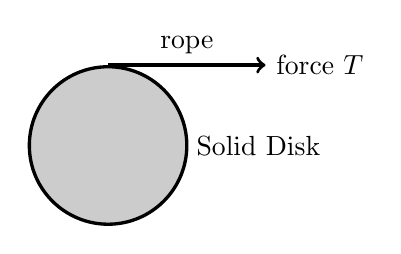
\begin{tikzpicture}
        \node[draw=black,very thick,fill=white!80!black,circle,minimum size=2cm] (A) at (0,0) {};
        \node[anchor=west,xshift=1cm] at (A) {Solid Disk};
        \draw[very thick,->] (A.north) -- ++ (0:2cm) node[pos=0.5,anchor=south] {rope} node[pos=1.0,anchor=west] {force $T$};
    \end{tikzpicture}
    \end{center}
    After the disk has accelerated some distance,
        determine the ratio of the translational $KE$ to total $KE$ of the disk,
    \begin{displaymath}
        \frac{KE_{translational}}{KE_{total}} =
    \end{displaymath}
    \begin{multicols}{3}
    \begin{choices}
        \wrongchoice{$\dfrac{1}{MR^2}$}
        \wrongchoice{$\dfrac{MR^2}{1}$}
        \wrongchoice{$\dfrac{1}{3MR^2}$}
      \correctchoice{$\dfrac{1}{MR^2+I}$}
        \wrongchoice{$\dfrac{MR^2}{MR^2+I}$}
    \end{choices}
    \end{multicols}
\end{question}
}

\element{aapt}{ %% Olympiad-A6
\begin{question}{olympiad-2014-q15}
    The maximum torque output from the engine of a new experimental car of mass $m$ is $\tau$.
    The maximum rotational speed of the engine is $\omega$.
    The engine is designed to provide a constant power output $P$.
    The engine is connected to the wheels via a perfect transmission
        that can smoothly trade torque for speed with no power loss.
    The wheels have a radius $R$,
        and the coefficient of static friction between the wheels and the road is $\mu$.
    %% Start Question
    What is the maximum sustained speed $v$ the car can drive up a \ang{30} incline?
    Assume no frictional losses and assume $\mu$ is large enough so that the tires do not slip.
    \begin{multicols}{2}
    \begin{choices}
      \correctchoice{$v=\dfrac{2P}{mg}$}
        \wrongchoice{$v=\dfrac{2P}{\sqrt{3}mg}$}
        \wrongchoice{$v=\dfrac{2P}{\mu mg}$}
        \wrongchoice{$v=\dfrac{\tau\omega}{mg}$}
        \wrongchoice{$v=\dfrac{\tau\omega}{\mu mg}$}
    \end{choices}
    \end{multicols}
\end{question}
}

\element{aapt}{ %% Olympiad-A5
\begin{question}{olympiad-2014-q16}
    An object of mass $m_1$ initially moving at speed $v_0$
        collides with an object of mass $m_2 = \alpha m_1$,
        where $\alpha <1$, that is initially at rest.
    The collision could be completely elastic, completely inelastic,
        or partially inelastic.
    After the collision the two objects move at speeds $v_1$ and $v_2$.
    Assume that the collision is one dimensional,
        and that object one cannot pass through object two.
    After the collision, the speed ratio $r_1 = \dfrac{v_1}{v_0}$ of object 1 is bounded by:
    \begin{choices}
        \wrongchoice{$\dfrac{1-\alpha}{1+\alpha} \leq r_1 \leq 1$}
      \correctchoice{$\dfrac{1-\alpha}{1+\alpha} \leq r_1 \leq \dfrac{1}{1+\alpha}$}
        \wrongchoice{$\dfrac{\alpha}{1+\alpha} \leq r_1 \leq 1$}
        \wrongchoice{$0 \leq r_1 \leq \dfrac{2\alpha}{1+\alpha}$}
        \wrongchoice{$\dfrac{1}{1+\alpha} \leq r_1 \leq \dfrac{2}{1+\alpha}$}
    \end{choices}
\end{question}
}

\element{aapt}{ %% Olympiad-A7
\begin{question}{olympiad-2014-q17}
    A spherical cloud of dust in space has a uniform density $\rho_0$ and a radius $R_0$.
    The gravitational acceleration of free fall at the surface
        of the cloud due to the mass of the cloud is $g_0$.
    A process occurs (heat expansion) that causes the cloud to suddenly grow to a radius $2R_0$,
        while maintaining a uniform (but not constant) density.
    The gravitational acceleration of free fall at a point $R_0$
        away from the center of the cloud due to the mass of the cloud is now:
    \begin{multicols}{3}
    \begin{choices}
        \wrongchoice{$\dfrac{1}{32} g_0$}
        \wrongchoice{$\dfrac{1}{16} g_0$}
      \correctchoice{$\dfrac{1}{8} g_0$}
        \wrongchoice{$\dfrac{1}{4} g_0$}
        \wrongchoice{$\dfrac{1}{2} g_0$}
    \end{choices}
    \end{multicols}
\end{question}
}

\element{aapt}{ %% Olympiad-A3
\begin{question}{olympiad-2014-q18}
    Consider the following diagram of a box and two weight scales.
    Scale $A$ supports the box via a massless rope.
    A pulley is attached to the top of the box;
        a second massless rope passes over the pulley,
        one end is attached to the box and the other end to scale $B$.
    The two scales read indicate the tensions $T_A$ and $T_B$ in the ropes.
    Originally scale $A$ reads \SI{30}{\newton} and scale $B$ reads \SI{20}{\newton}.
    \begin{center}
        %% NOTE: tikz?
        \includegraphics[keepaspectratio,scale=0.6]{Olympiad2014-Q18}
    \end{center}
    If an additional force pulls down on scale $B$ so that the reading increases to
        \SI{30}{\newton}, what will be the new reading on scale $A$?
    \begin{multicols}{3}
    \begin{choices}
        \wrongchoice{\SI{35}{\newton}}
      \correctchoice{\SI{40}{\newton}}
        \wrongchoice{\SI{45}{\newton}}
        \wrongchoice{\SI{50}{\newton}}
        \wrongchoice{\SI{60}{\newton}}
    \end{choices}
    \end{multicols}
\end{question}
}

\element{aapt}{ %% Olympiad-A3
\begin{question}{olympiad-2014-q19}
    A helicopter is flying horizontally at constant speed.
    A perfectly flexible uniform cable is suspended beneath the helicopter;
        air friction on the cable is not negligible.
    %% Start Question
    Which of the following diagrams best shows the shape of the cable
        as the helicopter flies through the air to the right?
    \begin{multicols}{2}
    \begin{choices}
        %% tikz?
        \AMCboxDimensions{down=-2cm}
        \wrongchoice{\includegraphics[keepaspectratio,scale=1.0]{Olympiad2014-Q19-A}}
      \correctchoice{\includegraphics[keepaspectratio,scale=1.0]{Olympiad2014-Q19-B}}
        \wrongchoice{\includegraphics[keepaspectratio,scale=1.0]{Olympiad2014-Q19-C}}
        \wrongchoice{\includegraphics[keepaspectratio,scale=1.0]{Olympiad2014-Q19-D}}
        \wrongchoice{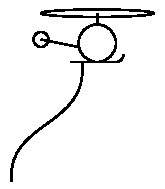
\includegraphics[keepaspectratio,scale=1.0]{Olympiad2014-Q19-E}}
    \end{choices}
    \end{multicols}
\end{question}
}

\element{aapt}{ %% Olympiad-A6
\begin{question}{olympiad-2014-q20}
    A crew of scientists has built a new space station.
    The space station is shaped like a wheel of radius $R$,
        with essentially all its mass $M$ at the rim.
    When the crew arrives, the station will be set rotating at a rate that
        causes an object at the rim to have radial acceleration $g$, thereby simulating
    Earth's surface gravity.
    This is accomplished by two small rockets, each with thrust $T$ newtons,
        mounted on the station's rim.
    How long a time $t$ does one need to fire the rockets to achieve the desired condition?
    \begin{multicols}{2}
    \begin{choices}
        \wrongchoice{$t=\dfrac{\sqrt{g R^3} M}{2T}$}
      \correctchoice{$t=\dfrac{\sqrt{g R} M}{2T}$}
        \wrongchoice{$t=\dfrac{\sqrt{g R} M}{T}$}
        \wrongchoice{$t=\sqrt{\dfrac{g R}{\pi}}\dfrac{M}{T}$}
        \wrongchoice{$t=\dfrac{\sqrt{g R}M}{\pi T}$}
    \end{choices}
    \end{multicols}
\end{question}
}

\element{aapt}{ %% Olympiad-A6
\begin{question}{olympiad-2014-q21}
    Two pulleys (shown in figure) are made of the same metal with density $\rho$.
    Pulley $A$ is a uniform disk with radius $R$.
    Pulley $B$ is identical except a circle of $\frac{R}{2}$ is removed from the center.
    When two boxes $M=\alpha m$, where $\alpha>1$,
        are connected over the pulleys through a massless rope and move without slipping,
        what is the ratio between the accelerations in system $A$ and $B$?
    \begin{center}
    \begin{tikzpicture}
        \begin{scope}[xshift=+2cm]
            %% Labels
            \node[anchor=south]at (0,1em) {Pulley $B$};
            %% Ceiling
            \node[anchor=south,fill,pattern=north east lines,minimum width=3cm, minimum height=0.05cm] at (-0.5,0) {};
            \draw (-2,0) -- (1,0);
            %% Pulley
            \draw[fill=white!50!black] (0,-1) circle (0.75);
            \draw[fill=white] (0,-1) circle (0.38);
            \draw[fill=white!90!black] (-0.3,0) -- (-0.10,-1.1) arc(190:350:0.10) -- (0.3,0) --cycle;
            \draw[fill] (0,-1) circle (1.5pt);
            %% Masses
            \node[draw,fill=white!90!black,rectangle,rounded corners=1ex,minimum size=1cm,anchor=north] (A) at (-0.75,-3) {$m$};
            \node[draw,fill=white!90!black,rectangle,rounded corners=1ex,minimum size=1.414cm,anchor=north] (B) at (0.75,-2.5) {$M$};
            %% Rope
            \draw[thick] (A.north) -- (-0.75,-1.0) arc(180:0:0.75) -- (B.north);
        \end{scope}
        \begin{scope}[xshift=-2cm]
            %% Labels
            \node[anchor=south] at (0,1em) {Pulley $A$};
            %% Ceilin3737
            \node[anchor=south,fill,pattern=north east lines,minimum width=3cm, minimum height=0.05cm] at (+0.5,0) {};
            \draw (-1,0) -- (2,0);
            %% Pulley
            \draw[fill=white!50!black] (0,-1) circle (0.75);
            \draw[fill=white!90!black] (-0.3,0) -- (-0.2,-1.1) arc(190:350:0.2) -- (0.3,0) --cycle;
            \draw[fill] (0,-1) circle (1.5pt);
            %% Masses
            \node[draw,fill=white!90!black,rectangle,rounded corners=1ex,minimum size=1cm,anchor=north] (A) at (-0.75,-3) {$m$};
            \node[draw,fill=white!90!black,rectangle,rounded corners=1ex,minimum size=1.414cm,anchor=north] (B) at (0.75,-2.5) {$M$};
            %% Rope
            \draw[thick] (A.north) -- (-0.75,-1.0) arc(180:0:0.75) -- (B.north);
        \end{scope}
    \end{tikzpicture}
    \end{center}
    The mass of pulley $A$ is $M+m$.
    \begin{multicols}{2}
    \begin{choices}
      \correctchoice{$\dfrac{a_A}{a_B} = \dfrac{47}{48}$}
        \wrongchoice{$\dfrac{a_A}{a_B} = \dfrac{31}{32}$}
        \wrongchoice{$\dfrac{a_A}{a_B} = \dfrac{15}{16}$}
        \wrongchoice{$\dfrac{a_A}{a_B} = \dfrac{9}{16}$}
        \wrongchoice{$\dfrac{a_A}{a_B} = \dfrac{3}{4}$}
    \end{choices}
    \end{multicols}
\end{question}
}

\element{aapt}{ %% Olympiad-A7
\begin{question}{olympiad-2014-q22}
    A body of mass $M$ and a body of mass $m\ll M$ are in circular orbits
        about their center of mass under the influence of their
        mutual gravitational attraction to each other.
    The distance between the bodies is $R$, which is much larger than the size of either body.
    %% Start Question
    A small amount of matter $\delta \ll m$ is removed from the body of mass $m$
        and transferred to the body of mass $M$.
    The transfer is done in such a way so that the orbits of the two bodies remain circular,
        and remain separated by a distance $R$.
    Which of the following statements is correct?
    \begin{choices}
        \wrongchoice{The gravitational force between the two bodies increases.}
        \wrongchoice{The gravitational force between the two bodies remains constant.}
        \wrongchoice{The total angular momentum of the system increases.}
        \wrongchoice{The total angular momentum of the system remains constant.}
      \correctchoice{The period of the orbit of two bodies remains constant.}
    \end{choices}
\end{question}
}

\element{aapt}{ %% Olympiad-A5
\begin{question}{olympiad-2014-q23}
    A \SI{100}{\kilo\gram} astronaut carries a launcher loaded with a
        \SI{10}{\kilo\gram} bowling ball;
        the launcher and the astronaut's spacesuit have negligible mass.
    The astronaut discovers that firing the launcher results in the ball
        moving away from her at a relative speed of \SI{50}{\meter\per\second}.
    %% Start question
    What is the impulse delivered to the astronaut when firing the launcher?
    \begin{multicols}{2}
    \begin{choices}
      \correctchoice{\SI{455}{\newton\second}}
        \wrongchoice{\SI{500}{\newton\second}}
        \wrongchoice{\SI{550}{\newton\second}}
        \wrongchoice{\SI{5000}{\newton\second}}
        \wrongchoice{\SI{5500}{\newton\second}}
    \end{choices}
    \end{multicols}
\end{question}
}

\element{aapt}{ %% Olympiad-A5
\begin{question}{olympiad-2014-q24}
    A \SI{100}{\kilo\gram} astronaut carries a launcher loaded with a
        \SI{10}{\kilo\gram} bowling ball;
        the launcher and the astronaut's spacesuit have negligible mass.
    The astronaut discovers that firing the launcher results in the ball
        moving away from her at a relative speed of \SI{50}{\meter\per\second}.
    %% Start question
    The astronaut is now moving at \SI{10}{\meter\per\second}
        (as measured in a certain frame of reference).
    She wishes to fire the launcher so that her velocity turns through
        as large an angle as possible (in this frame of reference).
    What is this maximum angle?
    (\emph{Hint:} a diagram may be useful.)
    \begin{multicols}{3}
    \begin{choices}
        \wrongchoice{\ang{24.4}}
        \wrongchoice{\ang{26.6}}
      \correctchoice{\ang{27.0}}
        \wrongchoice{\ang{30.0}}
        \wrongchoice{\ang{180.0}}
    \end{choices}
    \end{multicols}
\end{question}
}

\element{aapt}{ %% Olymmpiad-A4
\begin{question}{olympiad-2014-q25}
    A block with mass $m$ is released from rest at the top of a frictionless ramp.
    The block starts at a height $h_1$ above the base of the ramp,
        slides down the ramp, and then up a second ramp.
    The coefficient of kinetic friction between the block and the second ramp is $\mu_k$.
    If both ramps make an angle of $\theta$ with the horizontal,
        to what height $h_2$ above the base of the second ramp will the block rise?
    \begin{choices}
      \correctchoice{$h_2 = \dfrac{h_1\sin\theta}{\mu_k \cos\theta + \sin\theta}$}
        \wrongchoice{$h_2 = \dfrac{h_1\sin\theta}{\mu_k + \sin\theta}$}
        \wrongchoice{$h_2 = \dfrac{h_1\sin\theta}{\mu_k \cos^2\theta + \sin\theta}$}
        \wrongchoice{$h_2 = \dfrac{h_1\sin\theta}{\mu_k \cos^2\theta + \sin^2\theta}$}
        \wrongchoice{$h_2 = \dfrac{h_1\sin\theta}{\mu_k \sin\theta + \cos\theta}$}
    \end{choices}
\end{question}
}


%% PhysicsOlympiad 2013 F=ma Exam
%%----------------------------------------
\element{aapt}{ %% Olympiad-A1
\begin{question}{olympiad-2013-q01}
    An observer stands on the side of the front of a stationary train.
    When the train starts moving with constant acceleration,
        it takes \SI{5}{\second} for the first car to pass the observer.
    How long will it take for the 10\textsuperscript{th} car to pass?
    \begin{multicols}{3}
    \begin{choices}
        %% T_10 - T_9 = \sqrt{10*5^2} - \sqrt{9*5^2}
        \wrongchoice{\SI{1.07}{\second}}
        \wrongchoice{\SI{0.98}{\second}}
        \wrongchoice{\SI{0.91}{\second}}
        \wrongchoice{\SI{0.86}{\second}}
      \correctchoice{\SI{0.81}{\second}}
    \end{choices}
    \end{multicols}
\end{question}
}

\element{aapt}{ %% Olympiad-A5
\begin{question}{olympiad-2013-q02}
    Jordi stands \SI{20}{\meter} from a wall and Diego stands \SI{10}{\meter} from the same wall.
    Jordi throws a ball at an angle of \ang{30} above the horizontal,
        and it collides elastically with the wall.
    How fast does Jordi need to throw the ball so that Diego will catch it?
    Consider Jordi and Diego to be the same height,
        and both are on the same perpendicular line from the wall.
    \begin{multicols}{3}
    \begin{choices}
        \wrongchoice{\SI{11}{\meter\per\second}}
        \wrongchoice{\SI{15}{\meter\per\second}}
      \correctchoice{\SI{19}{\meter\per\second}}
        \wrongchoice{\SI{30}{\meter\per\second}}
        \wrongchoice{\SI{35}{\meter\per\second}}
    \end{choices}
    \end{multicols}
\end{question}
}

\element{aapt}{ %% Olympiad-A2
\begin{question}{olympiad-2013-q03}
    Tom throws a football to Wes, who is a distance $l$ away.
    Tom can control the time of flight $t$ of the ball by choosing any speed up to $v_{max}$
        and any launch angle between \ang{0} and \ang{90}.
    Ignore air resistance and assume Tom and Wes are at the same height.
    Which of the following statements is \emph{incorrect}?
    \begin{choices}
        %% remember R = \frac{v^2}{g}\sin 2\theta
        \wrongchoice{If $v_{max}<\sqrt{gl}$, the ball cannot reach Wes at all.}
        \wrongchoice{Assuming the ball can reach Wes, as $v_{max}$ increases with $l$ held fixed, the minimum value of $t$ decreases.}
        \wrongchoice{Assuming the ball can reach Wes, as $v_{max}$ increases with $l$ held fixed, the maximum value of $t$ increases.}
        \wrongchoice{Assuming the ball can reach Wes, as $l$ increases with $v_{max}$ held fixed, the minimum value of $t$ increases.}
      \correctchoice{Assuming the ball can reach Wes, as $l$ increases with $v_{max}$ held fixed, the maximum value of $t$ increases.}
    \end{choices}
\end{question}
}

\element{aapt}{ %% Olympiad-A6
\begin{question}{olympiad-2013-q04}
    The sign shown below consists of two uniform legs attached by a frictionless hinge.
    The coefficient of friction between the ground and the legs is $\mu$.
    Which of the following gives the maximum value of $\theta$ such that the sign will not collapse?
    \begin{center}
    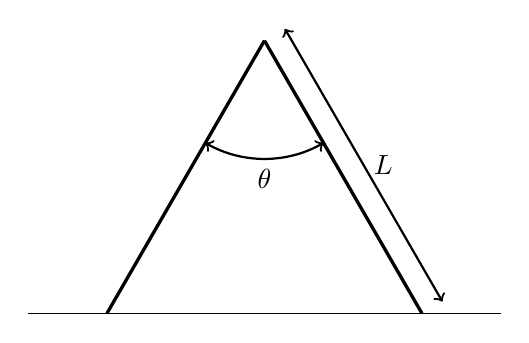
\begin{tikzpicture}
        %% Triangle
        \draw (-3,0) -- (3,0);
        \draw[very thick] (-2,0) -- ++ (60:4);
        \draw[very thick] (+2,0) -- ++ (120:4);
        %% Angle
        \draw[thick,<->] (-2,0) ++ (60:2.5) arc (240:300:1.5) node[pos=0.5,anchor=north] {$\theta$};
        %% Length
        \draw[thick,<->] (2,0) ++ (30:0.3) -- ++ (120:4) node[pos=0.5,anchor=west] {$L$};
    \end{tikzpicture}
    \end{center}
    \begin{multicols}{2}
    \begin{choices}
        \wrongchoice{$\sin\theta = 2\mu$}
        \wrongchoice{$\sin\dfrac{\theta}{2} = \dfrac{\mu}{2}$}
        \wrongchoice{$\tan\dfrac{\theta}{2} = \mu$}
        \wrongchoice{$\tan\theta = 2\mu$}
      \correctchoice{$\tan\dfrac{\theta}{2} = 2\mu$}
    \end{choices}
    \end{multicols}
\end{question}
}

\newcommand{\myOlympiadThirteenQzeroFive}{
\begin{tikzpicture}
    \begin{axis}[
        axis y line=left,
        axis x line=bottom,
        axis line style={->},
        xlabel={time},
        x unit=\si{\second},
        xtick={0,2,4,6,8,10,12,14,16,18,20,22,24,26},
        ylabel={scale reading},
        y unit=\si{\kilo\gram},
        ytick={0,20,40,60,80,100,120},
        %grid=major,
        xmin=0,xmax=26,
        ymin=0,ymax=120,
        width=0.90\columnwidth,
        height=0.45\columnwidth,
    ]
    \addplot[mark=\empty] plot coordinates { (0,80) (2,80) (2,60) (4,60) (4,80) (22,80) (22,100) (24,100) (24,80) (26,80) };
    \end{axis}
\end{tikzpicture}
}

\element{aapt}{ %% Olympiad-A3
\begin{question}{olympiad-2013-q05}
    A student steps onto a stationary elevator and stands on a bathroom scale.
    The elevator then travels from the top of the building to the bottom.
    The student records the reading on the scale as a function of time.
    \begin{center}
        \myOlympiadThirteenQzeroFive
    \end{center}
    At what time(s) does the student have maximum downward velocity?
    \begin{choices}
        \wrongchoice{At all times between \SI{2}{\second} and \SI{4}{\second}}
        \wrongchoice{At \SI{4}{\second} only}
      \correctchoice{At all times between \SI{4}{\second} and \SI{22}{\second}}
        \wrongchoice{At \SI{22}{\second} only}
        \wrongchoice{At all times between \SI{22}{\second} and \SI{24}{\second}}
    \end{choices}
\end{question}
}

\element{aapt}{ %% Olympiad-A3
\begin{question}{olympiad-2013-q06}
    A student steps onto a stationary elevator and stands on a bathroom scale.
    The elevator then travels from the top of the building to the bottom.
    The student records the reading on the scale as a function of time.
    \begin{center}
        \myOlympiadThirteenQzeroFive
    \end{center}
    How tall is the building?
    \begin{multicols}{3}
    \begin{choices}
        \wrongchoice{\SI{50}{\meter}}
        \wrongchoice{\SI{80}{\meter}}
      \correctchoice{\SI{100}{\meter}}
        \wrongchoice{\SI{150}{\meter}}
        \wrongchoice{\SI{400}{\meter}}
    \end{choices}
    \end{multicols}
\end{question}
}

\element{aapt}{ %% Olympiad-A5
\begin{question}{olympiad-2013-q07}
    A light car and a heavy truck have the same momentum.
    The truck weighs ten times as much as the car.
    How do their kinetic energies compare?
    \begin{choices}
        \wrongchoice{The truck's kinetic energy is larger by a factor of \num{100}}
        \wrongchoice{They truck's kinetic energy is larger by a factor of \num{10}}
        \wrongchoice{They have the same kinetic energy}
      \correctchoice{The car's kinetic energy is larger by a factor of \num{10}}
        \wrongchoice{The car's kinetic energy is larger by a factor of \num{100}}
    \end{choices}
\end{question}
}

\element{aapt}{ %% Olympiad-A5
\begin{question}{olympiad-2013-q08}
    A truck is initially moving at velocity $v$.
    The driver presses the brake in order to slow the truck to a stop.
    The brake applies a constant force $F$ to the truck.
    The truck rolls a distance $x$ before coming to a stop,
        and the time it takes to stop is $t$.
    %% Start question
    Which of the following expressions is equal the initial kinetic energy of the truck
        (i.e. the kinetic energy before the driver starts braking)?
    \begin{multicols}{2}
    \begin{choices}
      \correctchoice{$Fx$}
        \wrongchoice{$Fvt$}
        \wrongchoice{$Fxt$}
        \wrongchoice{$Ft$}
        \wrongchoice{Both $Fx$ and $FvT$ are correct}
    \end{choices}
    \end{multicols}
\end{question}
}

\element{aapt}{ %% Olympiad-A5
\begin{question}{olympiad-2013-q09}
    A truck is initially moving at velocity $v$.
    The driver presses the brake in order to slow the truck to a stop.
    The brake applies a constant force $F$ to the truck.
    The truck rolls a distance $x$ before coming to a stop,
        and the time it takes to stop is $t$.
    %% Start question
    Which of the following expressions is equal the initial momentum of the truck
        (i.e. the momentum before the driver starts braking)?
    \begin{multicols}{3}
    \begin{choices}
        \wrongchoice{$Fx$}
        \wrongchoice{$F\dfrac{t}{2}$}
        \wrongchoice{$Fxt$}
        \wrongchoice{$2Ft$}
      \correctchoice{$2F\dfrac{x}{v}$}
    \end{choices}
    \end{multicols}
\end{question}
}

\element{aapt}{ %% Olympiad-A6
\begin{question}{olympiad-2013-q10}
    Which of the following can be used to distinguish a solid ball
        from a hollow sphere of the same radius and mass?
    \begin{choices}
        \wrongchoice{Measurements of the orbit of a test mass around the object.}
      \correctchoice{Measurements of the time it takes the object to roll down an inclined plane.}
        \wrongchoice{Measurements of the tidal forces applied by the object to a liquid body.}
        \wrongchoice{Measurements of the behavior of the object as it floats in water.}
        \wrongchoice{Measurements of the force applied to the object by a uniform gravitational field.}
    \end{choices}
\end{question}
}

\element{aapt}{ %% Olympiad-A3
\begin{question}{olympiad-2013-q11}
    A right-triangular wooden block of mass $M$ is at rest on a table, as shown in figure.
    Two smaller wooden cubes, both with mass $m$,
        initially rest on the two sides of the larger block.
    As all contact surfaces are frictionless,
        the smaller cubes start sliding down the larger block while the block remains at rest.
    What is the normal force from the system to the table?
    \begin{center}
    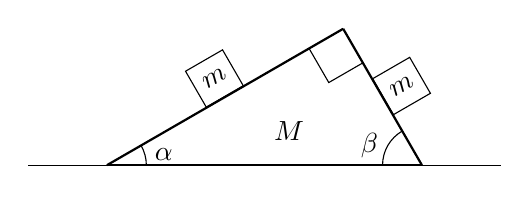
\begin{tikzpicture}
        %% Triangle
        \draw (-3,0) -- (3,0);
        \draw[thick] (-2,0) -- (2,0);
        \draw[thick] (-2,0) -- ++(30:3.464);
        \draw[thick] (+2,0) -- ++(120:2);
        \node[anchor=west] at (0,0.433) {$M$};
        %% Angles
        \draw (-2,0) ++ (0:0.5) arc (0:30:0.5) node[pos=0.5,anchor=west] {$\alpha$};
        \draw (+2,0) ++ (120:0.5) arc (120:180:0.5) node[pos=0.5,anchor=east] {$\beta$};
        \draw (1,1.732) ++ (-60:0.5) -- ++(210:0.5) -- ++(120:0.5);
        %% Blocks
        \node[draw,rectangle,minimum size=1.5em,rotate=30,anchor=south] at (-0.5,0.866) {$m$};
        \node[draw,rectangle,minimum size=1.5em,rotate=30,anchor=west] at (1.5,0.866) {$m$};
    \end{tikzpicture}
    \end{center}
    \begin{choices}
        \wrongchoice{$2mg$}
        \wrongchoice{$2mg + Mg$}
      \correctchoice{$mg + Mg$}
        \wrongchoice{$Mg + mg\left(\sin\alpha + \sin\beta\right)$}
        \wrongchoice{$Mg + mg\left(\cos\alpha + \cos\beta\right)$}
    \end{choices}
\end{question}
}

\element{aapt}{ %% Olympiad-A6
\begin{question}{olympiad-2013-q12}
    A spherical shell of mass $M$ and radius $R$ is completely filled with a frictionless fluid,
        also of mass $M$.
    It is released from rest,
        and then it rolls without slipping down an incline that makes an angle $theta$ with the horizontal.
    What will be the acceleration of the shell down the incline just after it is released?
    Assume the acceleration of free fall is $g$.
    The moment of inertia of a thin shell of radius $r$ and mass $m$ about the center of mass is $ =\frac{3}{2}mr^2$;
        the moment of inertia of a solid sphere of radius $r$ and mass $m$ about the center of mass is $I=\frac{2}{5} mr^2$.
    \begin{multicols}{2}
    \begin{choices}
        \wrongchoice{$a=g\sin\theta$}
      \correctchoice{$a=\dfrac{3g}{4}\sin\theta$}
        \wrongchoice{$a=\dfrac{g}{2}\sin\theta$}
        \wrongchoice{$a=\dfrac{3g}{8}\sin\theta$}
        \wrongchoice{$a=\dfrac{3g}{5}\sin\theta$}
    \end{choices}
    \end{multicols}
\end{question}
}

\element{aapt}{ %% Olympiad-A7
\begin{question}{olympiad-2013-q13}
    There is a ring outside of Saturn.
    In order to distinguish if the ring is actually a part of Saturn or is instead part of the satellites of Saturn,
        we need to know the relation between the velocity $v$ of each layer in the ring and the distance $R$ of the layer to the center of Saturn.
    Which of the following statements is correct?
    \begin{choices}
        %% v = \omega R, if connected
      \correctchoice{If $v\propto R$, then the layer is part of Saturn.}
        \wrongchoice{If $v^2\propto R$, then the layer is part of the satellites of Saturn.}
        \wrongchoice{If $v\propto \frac{1}{R}$, then the layer is part of Saturn.}
        %% v^2 = G M r, if in orbit
        \wrongchoice{If $v^2\propto \frac{1}{R}$, then the layer is part of Saturn.}
        \wrongchoice{If $v\propto R^2$, then the layer is part of the satellites of Saturn.}
    \end{choices}
\end{question}
}

\element{aapt}{ %% Olympiad-A5
\begin{question}{olympiad-2013-q14}
    A cart of mass $m$ moving at \SI{12}{\meter\per\second} to the right collides elastically with a cart of mass \SI{4.0}{\kilo\gram} that is originally at rest.
    After the collision,
        the cart of mass $m$ moves to the left with a velocity of \SI{6.0}{\meter\per\second}.
    Assuming an elastic collision in one dimension only,
        what is the velocity of the center of mass ($v_{cm}$) of the two carts before the collision?
    \begin{multicols}{2}
    \begin{choices}
        \wrongchoice{$v_{cm} = \SI{2.0}{\meter\per\second}$}
      \correctchoice{$v_{cm} = \SI{3.0}{\meter\per\second}$}
        \wrongchoice{$v_{cm} = \SI{6.0}{\meter\per\second}$}
        \wrongchoice{$v_{cm} = \SI{9.0}{\meter\per\second}$}
        \wrongchoice{$v_{cm} = \SI{18}{\meter\per\second}$}
    \end{choices}
    \end{multicols}
\end{question}
}

\element{aapt}{
\begin{question}{olympiad-2013-q15}
    A uniform rod is partially in water with one end suspended, as shown in figure.
    \begin{center}
        %% NOTE: tikz? draw=white
        \includegraphics[keepaspectratio,scale=1.0]{Olympiad2013-Q15}
    \end{center}
    The density of the rod is $5/9$ that of water.
    At equilibrium, what portion of the rod is above water?
    \begin{multicols}{3}
    \begin{choices}
        \wrongchoice{\num{0.25}}
        \wrongchoice{\num{0.33}}
        \wrongchoice{\num{0.5}}
      \correctchoice{\num{0.67}}
        \wrongchoice{\num{0.75}}
    \end{choices}
    \end{multicols}
\end{question}
}

\element{aapt}{ %% Olympiad-A7
\begin{question}{olympiad-2013-q16}
    %% \emph{Inspired by a problem from the 2012 International Physics Olympiad, Estonia}.
    A very large number of small particles forms a spherical cloud.
    Initially they are at rest, have uniform mass density per unit volume $\rho_0$,
        and occupy a region of radius $r_0$.
    The cloud collapses due to gravitation;
        the particles do not interact with each other in any other way.
    %% Start Questions
    How much time passes until the cloud collapses fully?
    (The constant \num{0.5427} is actually $\sqrt{\frac{3\pi}{32}}$.)
    \begin{multicols}{2}
    \begin{choices}
        %% Dimensional Analysis: time cannot depend on size
        \wrongchoice{$\dfrac{\num{0.5427}}{r_0^2 \sqrt{G\rho_0}}$}
        \wrongchoice{$\dfrac{\num{0.5427}}{r_0 \sqrt{G\rho_0}}$}
        \wrongchoice{$\dfrac{\num{0.5427}}{\sqrt{r_0 G\rho_0}}$}
      \correctchoice{$\dfrac{\num{0.5427}}{\sqrt{G\rho_0}}$}
        \wrongchoice{$\dfrac{\num{0.5427}}{\sqrt{G\rho_0}}r_0$}
    \end{choices}
    \end{multicols}
\end{question}
}

\element{aapt}{ %% Olympiad-A7
\begin{question}{olympiad-2013-q17}
    Two small, equal masses are attached by a lightweight rod.
    This object orbits a planet; the length of the rod is smaller than the radius of the orbit,
        but not negligible.
    The rod rotates about its axis in such a way that it remains vertical with respect to the planet.
    \begin{itemize}
        \item Is there a force in the rod?
            If so, is it tension or compression?
        \item Is the equilibrium stable, unstable, or neutral with respect to a small perturbation in the angle of the rod?
            (Assume this perturbation maintains the rate of rotation, so that in the co-rotating frame the rod is still stationary but at an angle to the vertical.)
    \end{itemize}
    \begin{center}
    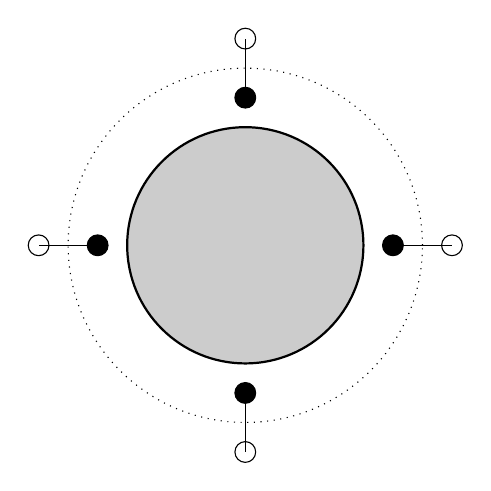
\begin{tikzpicture}[scale=0.75]
        \draw[thick,fill=white!80!black] (0,0) circle (2cm);
        \draw[dotted] (0,0) circle (3cm);
        \foreach \x in {0,90,180,270} {
            \draw[fill] (\x:2.5) circle (5pt);
            \draw (\x:3.5) circle (5pt);
            \draw (\x:2.5) -- (\x:3.5);
        }
    \end{tikzpicture}
    \end{center}
    \begin{choices}
        \wrongchoice{There is no force in the rod; the equilibrium is neutral.}
      \correctchoice{The rod is in tension; the equilibrium is stable.}
        \wrongchoice{The rod is in compression; the equilibrium is stable.}
        \wrongchoice{The rod is in tension; the equilibrium is unstable.}
        \wrongchoice{The rod is in compression; the equilibrium is unstable.}
    \end{choices}
\end{question}
}

\element{aapt}{ %% Olympiad-A5
\begin{question}{olympiad-2013-q18}
    Two point particles, each of mass \SI{1}{\kilo\gram}, begin in the state shown below.
    \begin{center}
    \begin{tikzpicture}[scale=0.9]
        \begin{axis}[
            xlabel={$x$},
            x unit=\si{\meter},
            xtick={-3,-2,-1,0,1,2,3},
            ylabel={$y$},
            y unit=\si{\meter},
            ytick={-3,-2,-1,0,1,2,3},
            grid=major,
            xmin=-3,xmax=3,
            ymin=-3,ymax=3,
            width=0.80\columnwidth,
            height=0.80\columnwidth,
        ]
        \draw[fill] (axis cs:1,1) circle (1.5pt);
        \draw[thick,->] (axis cs:1,1) -- (axis cs:0,1) node[pos=0.5,anchor=south] {\SI{1.0}{\meter\per\second}};
        \draw[fill] (axis cs:1,-1) circle (1.5pt);
        \draw[thick,->] (axis cs:1,-1) -- (axis cs:2,-1) node[pos=0.5,anchor=south] {\SI{1.0}{\meter\per\second}};
        \end{axis}
    \end{tikzpicture}
    \end{center}
    The system evolves through internal forces only.
    Which of the following could be the state after some time has passed?
    %% added to improve printing
    [Axis grid lines in options are identical to those in problem.]
    \begin{multicols}{2}
    \begin{choices}
        \AMCboxDimensions{down=-0.40\columnwidth}
        \wrongchoice{
            \begin{tikzpicture}[font=\small]
                \begin{axis}[
                    clip=false,
                    xlabel={},
                    xtick={-3,-2,-1,0,1,2,3},
                    xticklabels=\empty,
                    ylabel={},
                    ytick={-3,-2,-1,0,1,2,3},
                    yticklabels=\empty,
                    grid=major,
                    xmin=-3,xmax=3,
                    ymin=-3,ymax=3,
                    width=\columnwidth,
                    height=\columnwidth,
                ]
                \draw[fill] (axis cs:-1,0) circle (1.5pt);
                \draw[thick,->] (axis cs:-1,0) -- (axis cs:-1,-1) node[pos=1.0,anchor=north] {\SI{1.0}{\meter\per\second}};
                \draw[fill] (axis cs:1,0) circle (1.5pt);
                \draw[thick,->] (axis cs:1,0) -- (axis cs:1,1) node[pos=1.0,anchor=south] {\SI{1.0}{\meter\per\second}};
                \end{axis}
            \end{tikzpicture}
        }
        \wrongchoice{
            \begin{tikzpicture}[font=\small]
                \begin{axis}[
                    clip=false,
                    xlabel={},
                    xtick={-3,-2,-1,0,1,2,3},
                    xticklabels=\empty,
                    ylabel={},
                    ytick={-3,-2,-1,0,1,2,3},
                    yticklabels=\empty,
                    grid=major,
                    xmin=-3,xmax=3,
                    ymin=-3,ymax=3,
                    width=\columnwidth,
                    height=\columnwidth,
                ]
                \draw[fill] (axis cs:1,1) circle (1.5pt);
                \draw[thick,->] (axis cs:1,1) -- (axis cs:-1,1) node[pos=0.5,anchor=south] {\SI{2.0}{\meter\per\second}};
                \draw[fill] (axis cs:1,-1) circle (1.5pt);
                \end{axis}
            \end{tikzpicture}
        }
        \wrongchoice{
            \begin{tikzpicture}[font=\small]
                \begin{axis}[
                    clip=false,
                    xlabel={},
                    xtick={-3,-2,-1,0,1,2,3},
                    xticklabels=\empty,
                    ylabel={},
                    ytick={-3,-2,-1,0,1,2,3},
                    yticklabels=\empty,
                    grid=major,
                    xmin=-3,xmax=3,
                    ymin=-3,ymax=3,
                    width=\columnwidth,
                    height=\columnwidth,
                ]
                \draw[fill] (axis cs:2,0) circle (1.5pt);
                \draw[thick,->] (axis cs:2,0) -- (axis cs:1.303,0.707) node[pos=1.0,anchor=south] {\SI{1.0}{\meter\per\second}};
                \draw[fill] (axis cs:0,0) circle (1.5pt);
                \draw[thick,->] (axis cs:0,0) -- (axis cs:+0.707,-0.707) node[pos=0.5,anchor=north east] {\SI{1.0}{\meter\per\second}};
                \end{axis}
            \end{tikzpicture}
        }
        \wrongchoice{
            \begin{tikzpicture}[font=\small]
                \begin{axis}[
                    clip=false,
                    xlabel={},
                    xtick={-3,-2,-1,0,1,2,3},
                    xticklabels=\empty,
                    ylabel={},
                    ytick={-3,-2,-1,0,1,2,3},
                    yticklabels=\empty,
                    grid=major,
                    xmin=-3,xmax=3,
                    ymin=-3,ymax=3,
                    width=\columnwidth,
                    height=\columnwidth,
                ]
                \draw[fill] (axis cs:0,2) circle (1.5pt);
                \draw[thick,->] (axis cs:0,2) -- (axis cs:-1,2) node[pos=0.5,anchor=south] {\SI{1.0}{\meter\per\second}};
                \draw[fill] (axis cs:2,-2) circle (1.5pt);
                \draw[thick,->] (axis cs:2,-2) -- (axis cs:3,-2) node[pos=0.5,anchor=south] {\SI{1.0}{\meter\per\second}};
                \end{axis}
            \end{tikzpicture}
        }
        %% ANS is E
        \correctchoice{
            \begin{tikzpicture}[font=\small]
                \begin{axis}[
                    clip=false,
                    xlabel={},
                    xtick={-3,-2,-1,0,1,2,3},
                    xticklabels=\empty,
                    ylabel={},
                    ytick={-3,-2,-1,0,1,2,3},
                    yticklabels=\empty,
                    grid=major,
                    xmin=-3,xmax=3,
                    ymin=-3,ymax=3,
                    width=\columnwidth,
                    height=\columnwidth,
                ]
                \draw[fill] (axis cs:2,1) circle (1.5pt);
                \draw[thick,->] (axis cs:2,1) -- (axis cs:2,2) node[pos=0.5,anchor=east] {\SI{1.0}{\meter\per\second}};
                \draw[fill] (axis cs:0,-1) circle (1.5pt);
                \draw[thick,->] (axis cs:0,-1) -- (axis cs:0,-2) node[pos=0.5,anchor=west] {\SI{1.0}{\meter\per\second}};
                \end{axis}
            \end{tikzpicture}
        }
    \end{choices}
    \end{multicols}
\end{question}
}

\element{aapt}{ %% Olympiad-A8
\begin{question}{olympiad-2013-q19}
    %The following information applies to questions 19, 20, and 21.
    A simple pendulum experiment is constructed from a point mass $m$ attached to a pivot by a massless rod of length $L$ in a constant gravitational field.
    The rod is released from an angle $\theta_0 < \pi/2$ at rest and the period of motion is found to be $T_0$.
    Ignore air resistance and friction.
    %% Start question
    At what angle $\theta_g$ during the swing is the tension in the rod the greatest?
    \begin{choices}
        \wrongchoice{The tension is the greatest at the point $θ_g=\theta_0$.}
      \correctchoice{The tension is the greatest at the point $θ_g=0$.}
        \wrongchoice{The tension is the greatest at an angle $θ_g$ with $\theta < θ_g < θ_0$.}
        \wrongchoice{The tension is constant.}
        \wrongchoice{None of the provided are true for all values of $θ_0$ with $0 < θ_0 < \frac{\pi}{2}$.}
    \end{choices}
\end{question}
}

\element{aapt}{ %% Olympiad-A8
\begin{question}{olympiad-2013-q20}
    %The following information applies to questions 19, 20, and 21.
    A simple pendulum experiment is constructed from a point mass $m$ attached to a pivot by a massless rod of length $L$ in a constant gravitational field.
    The rod is released from an angle $\theta_0 < \pi/2$ at rest and the period of motion is found to be $T_0$.
    Ignore air resistance and friction.
    %% Start question
    What is the maximum value of the tension in the rod?
    \begin{multicols}{2}
    \begin{choices}
        \wrongchoice{$mg$}
        \wrongchoice{$2mg$}
        \wrongchoice{$\dfrac{mL\theta_0}{T_0^2}$}
        \wrongchoice{$mg \sin\theta_0$}
      \correctchoice{$mg\left( 3 - 2\cos\theta_0 \right)$}
    \end{choices}
    \end{multicols}
\end{question}
}

\element{aapt}{ %% Olympiad-A8
\begin{question}{olympiad-2013-q21}
    %The following information applies to questions 19, 20, and 21.
    A simple pendulum experiment is constructed from a point mass $m$ attached to a pivot by a massless rod of length $L$ in a constant gravitational field.
    The rod is released from an angle $\theta_0 < \pi/2$ at rest and the period of motion is found to be $T_0$.
    Ignore air resistance and friction.
    %% Start question
    The experiment is repeated with a new pendulum with a rod of length $4L$,
        using the same angle $\theta_0$, and the period of motion is found to be $T$.
    Which of the following statements is correct?
    \begin{choices}
      \correctchoice{$T = 2T_0$ regardless of the value of $\theta_0$.}
        \wrongchoice{$T > 2T_0$ with $T\approx{}2T_0$ if $\theta_0 \ll 1$.}
        \wrongchoice{$T < 2T_0$ with $T\approx{}2T_0$ if $\theta_0 \ll 1$.}
        \wrongchoice{$T > 2T_0$ for some values of $\theta_0$ and $T<2T_0$ for other values of $\theta_0$.}
        \wrongchoice{$T_0$ and $T$ are undefined because the motion is not periodic unless $\theta_0 \ll 1$.}
    \end{choices}
\end{question}
}

%% NOTE: graphics for A6
\element{aapt}{
\begin{question}{olympiad-2013-q22}
    A simplified model on the foot is shown.
    \begin{center}
        \includegraphics[keepaspectratio,width=\columnwidth]{Olympiad2013-Q22}
    \end{center}
    When a student of mass $m=\SI{60}{\kilo\gram}$ stands on a single toe,
        the tension $T$ in the Achilles Tendon is closest to:
    \begin{multicols}{2}
    \begin{choices}
        \wrongchoice{$T = \SI{600}{\newton}$}
        \wrongchoice{$T = \SI{1200}{\newton}$}
        \wrongchoice{$T = \SI{1800}{\newton}$}
      \correctchoice{$T = \SI{2400}{\newton}$}
        \wrongchoice{$T = \SI{3000}{\newton}$}
    \end{choices}
    \end{multicols}
\end{question}
}

\element{aapt}{ %% Olympiad-A4
\begin{question}{olympiad-2013-q23}
    %The following information applies to questions 23 and 24
    A man with mass $m$ jumps off of a high bridge with a bungee cord attached to his ankles.
    The man falls through a maximum distance $H$ at which point the bungee cord brings him to a momentary rest before he bounces back up.
    The bungee cord is perfectly elastic,
        obeying Hooke's force law with a spring constant $k$,
        and stretches from an original length of $L_0$ to a final length $L = L_0 + h$.
    The maximum tension in the Bungee cord is four times the weight of the man.
    %% Start question
    Determine the spring constant $k$.
    \begin{multicols}{2}
    \begin{choices}
        \wrongchoice{$k = \dfrac{mg}{h}$}
        \wrongchoice{$k = \dfrac{2mg}{h}$}
        \wrongchoice{$k = \dfrac{mg}{H}$}
        \wrongchoice{$k = \dfrac{2mg}{H}$}
      \correctchoice{$k = \dfrac{8mg}{H}$}
    \end{choices}
    \end{multicols}
\end{question}
}

\element{aapt}{ %% Olympiad-A4
\begin{question}{olympiad-2013-q24}
    %The following information applies to questions 23 and 24
    A man with mass $m$ jumps off of a high bridge with a bungee cord attached to his ankles.
    The man falls through a maximum distance $H$ at which point the bungee cord brings him to a momentary rest before he bounces back up.
    The bungee cord is perfectly elastic,
        obeying Hooke's force law with a spring constant $k$,
        and stretches from an original length of $L_0$ to a final length $L = L_0 + h$.
    The maximum tension in the Bungee cord is four times the weight of the man.
    %% Start question
    Find the maximum extension of the bungee cord $h$.
    \begin{multicols}{2}
    \begin{choices}
      \correctchoice{$h = \dfrac{1}{2}H$}
        \wrongchoice{$h = \dfrac{1}{4}H$}
        \wrongchoice{$h = \dfrac{1}{5}H$}
        \wrongchoice{$h = \dfrac{2}{5}H$}
        \wrongchoice{$h = \dfrac{1}{8}H$}
    \end{choices}
    \end{multicols}
\end{question}
}

\element{aapt}{ %% Olympiad-A3
\begin{question}{olympiad-2013-q25}
    A box with weight $W$ will slide down a \ang{30} incline at
        constant speed under the influence of gravity and friction alone.
    If instead a horizontal force $P$ is applied to the box,
        the box can be made to move up the ramp at constant speed.
    What is the magnitude of $P$?
    \begin{multicols}{2}
    \begin{choices}
        \wrongchoice{$P = \dfrac{1}{2} W$}
        \wrongchoice{$P = \dfrac{2}{\sqrt{3}} W$}
        \wrongchoice{$P = W$}
      \correctchoice{$P = \sqrt{3} W$}
        \wrongchoice{$P = 2 W$}
    \end{choices}
    \end{multicols}
\end{question}
}


%% PhysicsOlympiad 2012 F=ma Exam
%%----------------------------------------
\element{aapt}{ %% Olympiad-A1
\begin{question}{olympiad-2012-q01}
    Consider a dripping faucet, where the faucet is \SI{10}{\centi\meter} above the sink.
    The time between drops is such that when one drop hits the sink,
        one is in the air and another is about to drop.
    At what height above the sink will the drop in the air be right as a drop hits the sink?
    \begin{choices}
        \wrongchoice{Between \SI{0}{\centi\meter} and \SI{2}{\centi\meter}}
        \wrongchoice{Between \SI{2}{\centi\meter} and \SI{4}{\centi\meter}}
        \wrongchoice{Between \SI{4}{\centi\meter} and \SI{6}{\centi\meter}}
      \correctchoice{Between \SI{6}{\centi\meter} and \SI{8}{\centi\meter}}
        \wrongchoice{Between \SI{8}{\centi\meter} and \SI{10}{\centi\meter}}
    \end{choices}
\end{question}
}

\element{aapt}{ %% Olympiad-A2
\begin{question}{olympiad-2012-q02}
    A cannonball is launched with initial velocity of magnitude $v_0$
        over a horizontal surface.
    At what minimum angle $\theta_{min}$ above the horizontal should the
        cannonball be launched so that it rises to a height $H$
        which is larger than the horizontal distance $R$ that it will
        travel when it returns to the ground?
    \begin{choices}
      \correctchoice{$\theta_{min}=\ang{76}$}
        \wrongchoice{$\theta_{min}=\ang{72}$}
        \wrongchoice{$\theta_{min}=\ang{60}$}
        \wrongchoice{$\theta_{min}=\ang{45}$}
        \wrongchoice{There is no such angle, as $R>H$ for all range problems.}
    \end{choices}
\end{question}
}

\element{aapt}{ %% Olympiad-A6
\begin{question}{olympiad-2012-q03}
    An equilateral triangle is sitting on an inclined plane.
    Friction is too high for it to slide under any circumstance,
        but if the plane is sloped enough it can ``topple'' down the hill.
    What angle incline is necessary for it to start toppling?
    \begin{choices}
        \wrongchoice{30 degrees}
        \wrongchoice{45 degrees}
      \correctchoice{60 degrees}
        \wrongchoice{It will topple at any angle more than zero}
        \wrongchoice{It can never topple if it cannot slide}
    \end{choices}
\end{question}
}

\element{aapt}{ %% Olympiad-A5
\begin{question}{olympiad-2012-q04}
    A particle at rest explodes into three particles of equal mass
        in the absence of external forces.
    Two particles emerge at a right angle to each other with equal speed $v$.
    What is the speed of the third particle?
    \begin{multicols}{2}
    \begin{choices}
        \wrongchoice{$v$}
      \correctchoice{$\sqrt{2}v$}
        \wrongchoice{$2v$}
        \wrongchoice{$2\sqrt{2}v$}
        \wrongchoice{The third particle can have a range of different speeds.}
    \end{choices}
    \end{multicols}
\end{question}
}

\element{aapt}{ %% Olympiad-A5
\begin{question}{olympiad-2012-q05}
    A \SI{12}{\kilo\gram} block moving east at \SI{4}{\meter\per\second}
        collides head on with a \SI{6}{\kilo\gram} block that is moving
        west at \SI{2}{\meter\per\second}.
    The two blocks move together after the collision.
    What is the loss in kinetic energy in this collision?
    \begin{multicols}{3}
    \begin{choices}
        \wrongchoice{\SI{36}{\joule}}
        \wrongchoice{\SI{48}{\joule}}
        \wrongchoice{\SI{60}{\joule}}
      \correctchoice{\SI{72}{\joule}}
        \wrongchoice{\SI{96}{\joule}}
    \end{choices}
    \end{multicols}
\end{question}
}

\element{aapt}{ %% Olympiad-A2
\begin{question}{olympiad-2012-q06}
    Two cannons are arranged vertically, with the lower cannon pointing upward
        (towards the upper cannon) and the upper cannon pointing downward
        (towards the lower cannon), \SI{200}{\meter\per\second} above the lower cannon.
    Simultaneously, they both fire.
    The muzzle velocity of the lower cannon is \SI{25}{\meter\per\second}
        and the muzzle velocity of the upper cannon is \SI{55}{\meter\per\second}.
    \begin{center}
        \includegraphics[keepaspectratio,scale=0.8]{Olympiad2012-Q06}
    \end{center}
    How long after the cannons fire do the projectiles collide?
    \begin{multicols}{3}
    \begin{choices}
        \wrongchoice{\SI{2.2}{\second}}
      \correctchoice{\SI{2.5}{\second}}
        \wrongchoice{\SI{3.6}{\second}}
        \wrongchoice{\SI{6.7}{\second}}
        \wrongchoice{\SI{8.0}{\second}}
    \end{choices}
    \end{multicols}
\end{question}
}

\element{aapt}{ %% Olympiad-A2
\begin{question}{olympiad-2012-q07}
    Two cannons are arranged vertically, with the lower cannon pointing upward
        (towards the upper cannon) and the upper cannon pointing downward
        (towards the lower cannon), \SI{200}{\meter\per\second} above the lower cannon.
    Simultaneously, they both fire.
    The muzzle velocity of the lower cannon is \SI{25}{\meter\per\second}
        and the muzzle velocity of the upper cannon is \SI{55}{\meter\per\second}.
    \begin{center}
        \includegraphics[keepaspectratio,scale=0.8]{Olympiad2012-Q06}
    \end{center}
    How far beneath the top cannon do the projectiles collide?
    \begin{multicols}{3}
    \begin{choices}
        \wrongchoice{\SI{31}{\meter}}
        \wrongchoice{\SI{67}{\meter}}
        \wrongchoice{\SI{110}{\meter}}
        \wrongchoice{\SI{140}{\meter}}
      \correctchoice{\SI{170}{\meter}}
    \end{choices}
    \end{multicols}
\end{question}
}

\element{aapt}{ %% Olympiad-A4
\begin{question}{olympiad-2012-q08}
    A block of mass $m=\SI{3.0}{\kilo\gram}$ is moving on a horizontal surface
        towards a massless spring with spring constant $k=\SI{80.0}{\newton\per\meter}$.
    The coefficient of kinetic friction between the block and the
        surface is $\mu_k=\num{0.50}$.
    The block has a speed of \SI{2.0}{\meter\per\second} when it first
        comes in contact with the spring.
    How far will the spring be compressed?
    \begin{multicols}{3}
    \begin{choices}
        \wrongchoice{\SI{0.19}{\meter}}
      \correctchoice{\SI{0.24}{\meter}}
        \wrongchoice{\SI{0.39}{\meter}}
        \wrongchoice{\SI{0.40}{\meter}}
        \wrongchoice{\SI{0.61}{\meter}}
    \end{choices}
    \end{multicols}
\end{question}
}

\element{aapt}{ %% Olympiad-A7
\begin{question}{olympiad-2012-q09}
    A uniform spherical planet has radius $R$ and the acceleration due
        to gravity at its surface is $g$.
    What is the escape velocity of a particle from the planet's surface?
    \begin{multicols}{2}
    \begin{choices}
        \wrongchoice{$\frac{1}{2}\sqrt{gR}$}
        \wrongchoice{$\sqrt{gR}$}
      \correctchoice{$\sqrt{2gR}$}
        \wrongchoice{$2\sqrt{gR}$}
        \wrongchoice{The escape velocity cannot be expressed in terms of $g$ and $R$ alone.}
    \end{choices}
    \end{multicols}
\end{question}
}

\element{aapt}{ %% Olympiad-A6
\begin{question}{olympiad-2012-q10}
    Four objects are placed at rest at the top of an inclined plane
        and allowed to roll without slipping to the bottom in the
        absence of rolling resistance and air resistance.
    \begin{itemize}
        \item Object $A$ is a solid brass ball of diameter $d$.
        \item Object $B$ is a solid brass ball of diameter $2d$.
        \item Object $C$ is a hollow brass sphere of diameter $d$.
        \item Object $D$ is a solid aluminum ball of diameter $d$. (Aluminum is less dense than brass.)
    \end{itemize}
    The balls are placed so that their centers of mass all travel the same distance.
    In each case, the time of motion $T$ is measured.
    Which of the following statements is correct?
    \begin{choices}
        \wrongchoice{$T_B > T_C > T_A = T_D$}
        \wrongchoice{$T_A = T_B = T_C > T_D$}
        \wrongchoice{$T_B > T_A = T_C = T_D$}
      \correctchoice{$T_C > T_A = T_B = T_D$}
        \wrongchoice{$T_A = T_B = T_C = T_D$}
    \end{choices}
\end{question}
}

\element{aapt}{ %% Olympiad-A3
\begin{question}{olympiad-2012-q11}
    As shown below, Lily is using the rope through a fixed pulley
        to move a box with constant speed $v$.
    The kinetic friction coefficient between the box and the ground is $\mu<1$;
        assume that the fixed pulley is massless and there is no friction
        between the rope and the fixed pulley.
    Then, while the box is moving,
        which of the following statements is correct?
    \begin{center}
        \includegraphics[keepaspectratio,scale=0.8]{Olympiad2012-Q11}
    \end{center}
    \begin{choices}
        \wrongchoice{The magnitude of the force on the rope is constant.}
      \correctchoice{The magnitude of friction between the ground and the box is decreasing.}
        \wrongchoice{The magnitude of the normal force of the ground on the box is increasing.}
        \wrongchoice{The pressure of the box on the ground is increasing.}
        \wrongchoice{The pressure of the box on the ground is constant.}
    \end{choices}
\end{question}
}

\element{aapt}{ %% Olympiad-A6
\begin{question}{olympiad-2012-q12}
    A rigid hoop can rotate about the center.
    Two massless strings are attached to the hoop, one at $A$, the other at $B$.
    These strings are tied together at the center of the hoop at $O$,
        and a weight $G$ is suspended from that point.
    The strings have a fixed length, regardless of the tension,
        and the weight $G$ is only supported by the strings.
    Originally $OA$ is horizontal.
    \begin{center}
    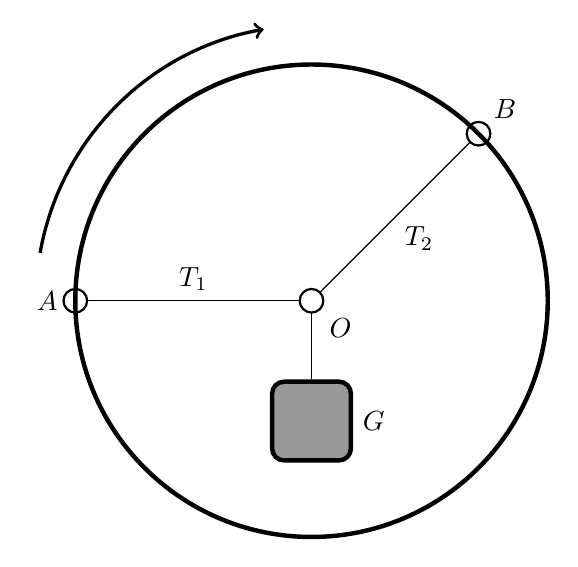
\begin{tikzpicture}
        \draw[ultra thick] (0,0) circle (3cm);
        \draw[thick] (0,0) circle (0.15cm);
        \node[anchor=north west] at (315:0.15cm) {$O$};
        %% 45 degree ring
        \draw[thick] (45:3) circle (0.15cm);
        \draw (45:0.15) -- (45:2.85) node[pos=0.5,anchor=north west] {$T_2$};
        \node[anchor=south west] at (45:3.1) {$B$};
        %% 180 degree ring
        \draw[thick] (180:3) circle (0.15cm);
        \draw (180:0.15cm) -- (180:2.85) node[pos=0.5,anchor=south] {$T_1$};
        \node[anchor=east] at (180:3.1) {$A$};
        %% Rotational direction
        \draw[very thick,->] (170:3.5) arc(170:100:3.5);
        %% handing mass
        \node[ultra thick,draw,fill=white!60!black,rounded corners=1ex,minimum size=1cm,anchor=north] (M) at (0,-1) {};
        \draw (M.north) -- (270:0.15cm);
        \node[anchor=west] at (M.east) {$G$};
    \end{tikzpicture}
    \end{center}
    Now, the outer hoop will start to slowly rotate \ang{90} clockwise
        until $OA$ will become vertical, while keeping the angle between
        the strings constant and keeping the object static.
    Which of the following statements about the tensions $T_1$ and $T_2$
        in the two strings is correct?
    \begin{choices}
        \wrongchoice{$T_1$ always decreases.}
        \wrongchoice{$T_1$ always increases.}
        \wrongchoice{$T_2$ always increases.}
      \correctchoice{$T_2$ will become zero at the end of the rotation.}
        \wrongchoice{$T_2$ first increases and then decreases.}
    \end{choices}
\end{question}
}

\element{aapt}{ %% Olympiad-A4
\begin{question}{olympiad-2012-q13}
    Shown below is a graph of the $x$ component of force versus position
        for a \SI{4.0}{\kilo\gram} cart constrained to move in one dimension on the $x$ axis.
    \begin{center}
    \begin{tikzpicture}
        \begin{axis}[
            axis y line=middle,
            axis x line=bottom,
            axis line style={->},
            xlabel={$x$},
            x unit=\si{\meter},
            xtick={-4,-2,0,2,4,6,8},
            minor x tick num=1,
            ylabel={$F$},
            y unit=\si{\newton},
            ytick={-2,0,2,4,6},
            minor x tick num=1,
            grid=major,
            xmin=-2,ymax=8,
            ymin=-4,xmax=8,
            width=0.95\columnwidth,
            height=0.618\columnwidth,
        ]
        \addplot[line width=1pt,domain=-4:1]{5};
        \addplot[line width=1pt,domain=1:8]{6 - x};
        \end{axis}
    \end{tikzpicture}
    \end{center}
    At $x=0$ the cart has a velocity of \SI{-3.0}{\meter\per\second}
        (in the negative direction).
    Which of the following is closest to the maximum speed of the cart?
    \begin{multicols}{2}
    \begin{choices}
        \wrongchoice{\SI{1.6}{\meter\per\second}}
        \wrongchoice{\SI{2.5}{\meter\per\second}}
        \wrongchoice{\SI{3.0}{\meter\per\second}}
        \wrongchoice{\SI{4.0}{\meter\per\second}}
      \correctchoice{\SI{4.2}{\meter\per\second}}
    \end{choices}
    \end{multicols}
\end{question}
}

\element{aapt}{
\begin{question}{olympiad-2012-q14}
    A uniform cylinder of radius a originally has a weight of \SI{80}{\newton}.
    After an off-axis cylinder hole at $2a/5$ was drilled through it,
        it weighs \SI{65}{\newton}.
    The axes of the two cylinders are parallel and their centers are at the same height.
    \begin{center}
    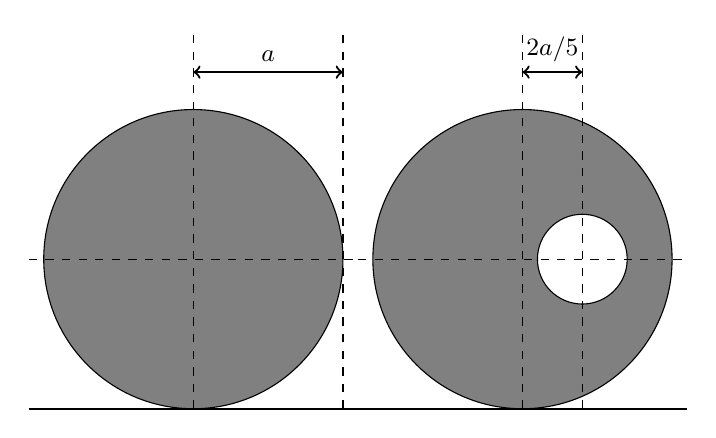
\begin{tikzpicture}[scale=0.95,font=\small]
        \begin{scope}[xshift=-2.2cm]
            %% cylinder
            \draw[fill=white!50!black] (0,0)  circle (2cm);
            %% Floor
            \draw[thick] (-2.2,-2) -- (2.2,-2);
            %% axis
            \draw[dashed] (-2.2,0) -- (2.2,0);
            \draw[dashed] (0,-2) -- (0,3);
            \draw[dashed] (2,-2) -- (2,3);
            %% Radius
            \draw[thick,<->] (0,2.5) -- (2,2.5) node[pos=0.5,anchor=south] {$a$};
        \end{scope}
        \begin{scope}[xshift=+2.2cm]
            %% cylinder
            \draw[fill=white!50!black] (0,0)  circle (2cm);
            \draw[fill=white] (0.8,0)  circle (0.6cm);
            %% Floor
            \draw[thick] (-2.2,-2) -- (2.2,-2);
            %% axis
            \draw[dashed] (-2.2,0) -- (2.2,0);
            \draw[dashed] (0,-2) -- (0,3);
            \draw[dashed] (0.8,-2) -- (0.8,3);
            %% Radius
            \draw[thick,<->] (0,2.5) -- (0.8,2.5) node[pos=0.5,anchor=south] {$2a/5$};
            \draw[dashed] (0.8,3) -- (0.8,3);
        \end{scope}
    \end{tikzpicture}
    \end{center}
    A force $T$ is applied to the top of the cylinder horizontally.
    In order to keep the cylinder is at rest,
        the magnitude of the force is closest to:
    \begin{multicols}{3}
    \begin{choices}
      \correctchoice{\SI{6}{\newton}}
        \wrongchoice{\SI{10}{\newton}}
        \wrongchoice{\SI{15}{\newton}}
        \wrongchoice{\SI{30}{\newton}}
        \wrongchoice{\SI{38}{\newton}}
    \end{choices}
    \end{multicols}
\end{question}
}

\element{aapt}{ %% Olympiad-A4
\begin{question}{olympiad-2012-q15}
    A car of mass $m$ has an engine that provides a constant power output $P$.
    Assuming no friction, what is the maximum constant speed $v_{max}$
        that this car can drive up a long incline that makes an angle θ with the horizontal?
    \begin{choices}
      \correctchoice{$v_{max}=\dfrac{P}{mg\sin\theta}$}
        \wrongchoice{$v_{max}=\dfrac{P^2\sin\theta}{mg}$}
        \wrongchoice{$v_{max}=\dfrac{1}{\sin\theta}\sqrt{\dfrac{2P}{mg}}$}
        \wrongchoice{There is no maximum constant speed.}
        \wrongchoice{The maximum constant speed depends on the length of the incline.}
    \end{choices}
\end{question}
}

\element{aapt}{ %% Olympiad-A8
\begin{question}{olympiad-2012-q16}
    Inside a cart that is accelerating horizontally at acceleration $\vec{a}$,
        there is a block of mass $M$ connected to two light springs of
        force constants $k_1$ and $k_2$.
    \begin{center}
    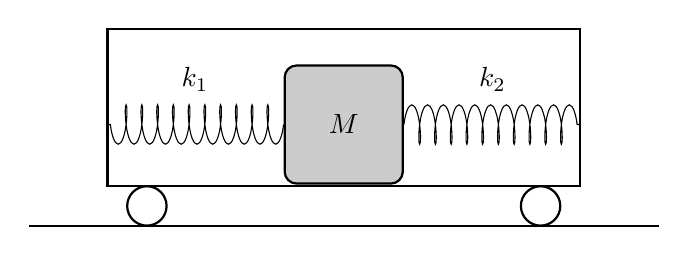
\begin{tikzpicture}
        %% Floor
        \draw[thick] (-4,0) -- (4,0);
        %% Cart
        \draw[thick] (-3,0.5) rectangle (3,2.5);
        %% Wheels
        \draw[thick] (-2.5,0.25) circle (0.25);
        \draw[thick] (+2.5,0.25) circle (0.25);
        %% Mass
        \node[thick,draw,minimum size=1.5cm,fill=white!80!black,rounded corners=1ex,anchor=south] (M) at (0,0.52) {$M$};
        %% spring
        \draw[decoration={aspect=0.2,segment length=2.0mm,amplitude=2.5mm,coil},decorate] (M.west) -- ++(180:2.25) node[pos=0.5,anchor=south,yshift=3mm] {$k_1$};
        \draw[decoration={aspect=0.2,segment length=2.0mm,amplitude=2.5mm,coil},decorate] (M.east) -- ++(0:2.25) node[pos=0.5,anchor=south,yshift=3mm] {$k_2$};
    \end{tikzpicture}
    \end{center}
    The block can move without friction horizontally.
    Find the vibration frequency of the block.
    \begin{choices}
        \wrongchoice{$\dfrac{1}{2\pi}\sqrt{\dfrac{k_1+k_2}{M} + a}$}
        \wrongchoice{$\dfrac{1}{2\pi}\sqrt{\dfrac{k_1 k_2}{\left(k_1+k_2\right)M}}$}
        \wrongchoice{$\dfrac{1}{2\pi}\sqrt{\dfrac{k_1 k_2}{\left(k_1+k_2\right)M} + a}$}
        \wrongchoice{$\dfrac{1}{2\pi}\sqrt{\dfrac{|k_1-k_2|}{M}}$}
      \correctchoice{$\dfrac{1}{2\pi}\sqrt{\dfrac{k_1+k_2}{M}}$}
    \end{choices}
\end{question}
}

\element{aapt}{ %% Olympiad-A8
\begin{question}{olympiad-2012-q17}
    Shown below is a log/log plot for the data collected of amplitude
        and period of oscillation for certain non-linear oscillator.
    \begin{center}
    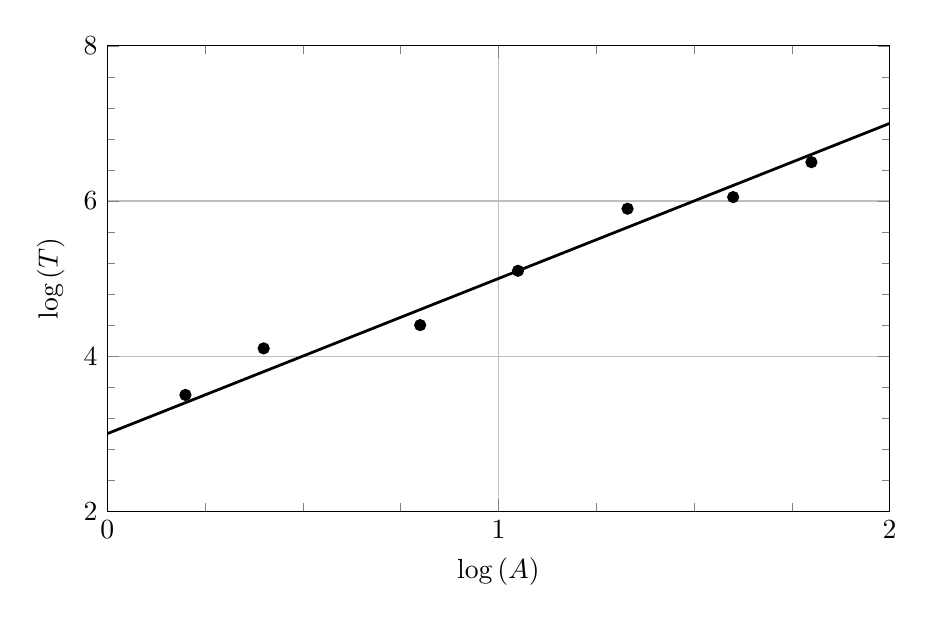
\begin{tikzpicture}
        \begin{axis}[
            xlabel={$\log\left(A\right)$},
            xtick={0,1,2},
            minor x tick num=3,
            ylabel={$\log\left(T\right)$},
            ytick={2,4,6,8},
            minor y tick num=4,
            grid=major,
            xmin=0,xmax=2,
            ymin=2,ymax=8,
            width=0.95\columnwidth,
            height=0.618\columnwidth,
        ]
        \addplot[line width=1pt,domain=0:2]{3 + 2*x};
        \addplot[mark=*,only marks] plot coordinates { (0.20,3.5) (0.4,4.1) (0.80,4.4) (1.05,5.1) (1.33,5.9) (1.6,6.05) (1.8,6.5) };
        \end{axis}
    \end{tikzpicture}
    \end{center}
    According to the data,
        the relationship between period $T$ and amplitude $A$ is best given by:
    \begin{choices}
      \correctchoice{$T=\num{1000}A^2$}
        \wrongchoice{$T=\num{1000}A^3$}
        \wrongchoice{$T=2A+3$}
        \wrongchoice{$T=3\sqrt{A}$}
        \wrongchoice{Period is independent of amplitude for oscillating systems}
    \end{choices}
\end{question}
}

\element{aapt}{ %% Olympiad-A8
\begin{question}{olympiad-2012-q18}
    A mass hangs from the ceiling of a box by an ideal spring.
    With the box held fixed,
        the mass is given an initial velocity and oscillates with purely vertical motion.
    When the mass reaches the lowest point of its motion,
        the box is released and allowed to fall.
    To an observer inside the box,
        which of the following quantities does not change when the box is released?
    Ignore air resistance.
    \begin{choices}
        \wrongchoice{The amplitude of the oscillation}
      \correctchoice{The period of the oscillation}
        \wrongchoice{The maximum speed reached by the mass}
        \wrongchoice{The height at which the mass reaches its maximum speed}
        \wrongchoice{The maximum height reached by the mass}
    \end{choices}
\end{question}
}

\element{aapt}{ %% Olympiad-A4
\begin{question}{olympiad-2012-q19}
    A \SI{1 500}{\watt} motor is used to pump water a vertical height of
        \SI{2.0}{\meter} out of a flooded basement through a cylindrical pipe.
    The water is ejected though the end of the pipe at a speed of \SI{2.5}{\meter\per\second}.
    Ignoring friction and assuming that all of the energy of the motor goes to the water,
        which of the following is the closest to the radius of the pipe?
    The density of water is $\rho=\SI{1000}{\kilo\gram\per\meter\cubed}$.
    \begin{multicols}{3}
    \begin{choices}
        \wrongchoice{\SI{1/3}{\centi\meter}}
        \wrongchoice{\SI{1}{\centi\meter}}
        \wrongchoice{\SI{3}{\centi\meter}}
      \correctchoice{\SI{10}{\centi\meter}}
        \wrongchoice{\SI{30}{\centi\meter}}
    \end{choices}
    \end{multicols}
\end{question}
}

\element{aapt}{
\begin{question}{olympiad-2012-q20}
    A container of water is sitting on a scale.
    Originally, the scale reads $M_1=\SI{45}{\kilo\gram}$.
    A block of wood is suspended from a second scale;
        originally the scale read $M_2=\SI{12}{\kilo\gram}$.
    The density of wood is \SI{0.60}{\gram\per\centi\meter\cubed};
        the density of the water is \SI{1.00}{\gram\per\centi\meter\cubed}.
    The block of wood is lowered into the water until half of the block is beneath the surface.
    What is the resulting reading on the scales?
    \begin{center}
        \includegraphics[keepaspectratio,scale=1.0]{Olympiad2012-Q20}
    \end{center}
    \begin{choices}
        \wrongchoice{$M_1=\SI{45}{\kilo\gram}$ and $M_2=\SI{2}{\kilo\gram}$.}
        \wrongchoice{$M_1=\SI{45}{\kilo\gram}$ and $M_2=\SI{6}{\kilo\gram}$.}
        \wrongchoice{$M_1=\SI{45}{\kilo\gram}$ and $M_2=\SI{10}{\kilo\gram}$.}
        \wrongchoice{$M_1=\SI{55}{\kilo\gram}$ and $M_2=\SI{6}{\kilo\gram}$.}
      \correctchoice{$M_1=\SI{55}{\kilo\gram}$ and $M_2=\SI{2}{\kilo\gram}$.}
    \end{choices}
\end{question}
}

%% NOTE: tikz for A4
\element{aapt}{
\begin{question}{olympiad-2012-q21}
    A spring system is set up as follows:
        a platform with a weight of \SI{10}{\newton} is on top of two springs,
        each with spring constant \SI{75}{\newton\per\meter}.
    On top of the platform is a third spring with spring constant \SI{75}{\newton\per\meter}.
    \begin{center}
    \begin{tikzpicture}
        %% Table And floor
        \draw[thick,fill=white!80!black] (-3,0) rectangle (3,0.2);
        \draw[thick] (-3,-2) -- (+3,-2);
        %% springs
        \draw[decoration={aspect=0.2,segment length=2.0mm,amplitude=2.5mm,coil},decorate] (0,0.2) -- ++(90:2);
        \draw[decoration={aspect=0.2,segment length=2.0mm,amplitude=2.5mm,coil},decorate] (-2,0) -- ++(270:2);
        \draw[decoration={aspect=0.2,segment length=2.0mm,amplitude=2.5mm,coil},decorate] (+2,0) -- ++(270:2);
        %% original height
        \draw[<->,thick] (-4.5,-2) -- (-4.5,2.2) node[pos=0.5,anchor=center,fill=white,text centered,text width=5em] {Original Height};
        %% ball is placed here
        \draw[dashed] (-4.6,2.2) -- (0.5,2.2);
        \draw[dashed] (-4.6,0) -- (-3,0);
        \draw[thick,<-] (0,2.2) -- ++(20:1) node[anchor=south] {The ball is placed here};
    \end{tikzpicture}
    \end{center}
    If a ball with a weight of \SI{5.0}{\newton} is then fastened to the
        top of the third spring and then slowly lowered,
        by how much does the height of the spring system change?
    \begin{multicols}{3}
    \begin{choices}
        \wrongchoice{\SI{0.033}{\meter}}
        \wrongchoice{\SI{0.067}{\meter}}
      \correctchoice{\SI{0.100}{\meter}}
        \wrongchoice{\SI{0.133}{\meter}}
        \wrongchoice{\SI{0.600}{\meter}}
    \end{choices}
    \end{multicols}
\end{question}
}

\element{aapt}{
\begin{question}{olympiad-2012-q22}
    The softest audible sound has an intensity of $I_0=\SI{e-12}{\watt\per\meter\squared}$.
    In terms of the fundamental units of kilograms,
        meters, and seconds, this is equivalent to:
    \begin{choices}
      \correctchoice{$I_0=\SI{e-12}{\kilo\gram\per\second\cubed}$}
        \wrongchoice{$I_0=\SI{e-12}{\kilo\gram\per\second}$}
        \wrongchoice{$I_0=\SI{e-12}{\kilo\gram\squared\meter\per\second}$}
        \wrongchoice{$I_0=\SI{e-12}{\kilo\gram\squared\meter\per\second\squared}$}
        \wrongchoice{$I_0=\SI{e-12}{\kilo\gram\per\meter\per\second\cubed}$}
    \end{choices}
\end{question}
}

\element{aapt}{ %% Olympiad-A7
\begin{question}{olympiad-2012-q23}
    Which of the following sets of equipment \emph{cannot} be used to
        measure the local value of the acceleration due to gravity ($g$)?
    \begin{choices}
        \wrongchoice{A spring scale (which reads in force units) and a known mass.}
        \wrongchoice{A rod of known length, an unknown mass, and a stopwatch.}
      \correctchoice{An inclined plane of known inclination, several carts of different known masses, and a stopwatch.}
        \wrongchoice{A launcher which launches projectiles at a known speed, a projectile of known mass, and a meter stick.}
        \wrongchoice{A motor with a known output power, a known mass, a piece of string of unknown length, and a stopwatch.}
    \end{choices}
\end{question}
}

\element{aapt}{ %% Olympiad-A6
\begin{question}{olympiad-2012-q24}
    Three point masses $m$ are attached together by identical springs.
    When placed at rest on a horizontal surface the masses
        form a triangle with side length $l$.
    When the assembly is rotated about its center at angular velocity $\omega$,
        the masses form a triangle with side length $2l$.
    What is the spring constant $k$ of the springs?
    \begin{multicols}{3}
    \begin{choices}
        \wrongchoice{$2m\omega^2$}
        \wrongchoice{$\dfrac{2}{\sqrt{3}}m\omega^2$}
      \correctchoice{$\dfrac{2}{3}m\omega^2$}
        \wrongchoice{$\dfrac{1}{\sqrt{3}}m\omega^2$}
        \wrongchoice{$\dfrac{1}{3}m\omega^2$}
    \end{choices}
    \end{multicols}
\end{question}
}

%% NOTE: tikz for A7
\element{aapt}{
\begin{question}{olympiad-2012-q25}
    Consider the two orbits around the sun shown below.
    Orbit $P$ is circular with radius $R$, orbit $Q$ is elliptical such
        that the farthest point $b$ is between $2R$ and $3R$,
        and the nearest point $a$ is between $\frac{R}{3}$ and $\frac{R}{2}$.
    Consider the magnitudes of the velocity of the circular orbit $v_c$,
        the velocity of the comet in the elliptical orbit at the farthest point $v_b$,
        and the velocity of the comet in the elliptical orbit at the nearest point $v_a$.
    Which of the following rankings is correct?
    \begin{center}
    %\includegraphics[keepaspectratio,scale=0.8]{Olympiad2012-Q25}
    \begin{tikzpicture}
        %% TODO: foci in terms of major and minor axis
        %% Circle: Orbit P
        \draw[fill=white!70!black] (0,0) circle (0.1cm);
        \draw[thick,->] (0,0)-- (45:2cm) node[pos=0.5,anchor=north west] {$R$};
        %% Ellipse: Orbit Q
        %% Points: A, B, C
        \draw (90:2) -- ++ (0:1.5) node[pos=0.5,anchor=south] {$v_c$};
    \end{tikzpicture}
    \end{center}
    \begin{multicols}{2}
    \begin{choices}
        \wrongchoice{$v_b > v_c > 2v_a$}
        \wrongchoice{$2v_c > v_b > v_a$}
      \correctchoice{$10v_b > v_a > v_c$}
        \wrongchoice{$v_c > v_a > 4v_b$}
        \wrongchoice{$2v_a > \sqrt{2}v_b > v_c$}
    \end{choices}
    \end{multicols}
\end{question}
}


%% PhysicsOlympiad 2011 F=ma Exam
%%----------------------------------------
\element{aapt}{ %% Olympiad-A1
\begin{question}{olympiad-2011-q01}
    A cyclist travels at a constant speed of \SI{22.0}{\kilo\meter\per\hour}
        except for a \SI{20}{\minute} stop.
    The cyclist's average speed was \SI{17.5}{\kilo\meter\per\hour}.
    How far did the cyclist travel?
    \begin{multicols}{2}
    \begin{choices}
        %% d = v \frac{ \bar{v} T }{ v - \bar{v} }
      \correctchoice{\SI{28.5}{\kilo\meter}}
        \wrongchoice{\SI{30.3}{\kilo\meter}}
        \wrongchoice{\SI{31.2}{\kilo\meter}}
        \wrongchoice{\SI{36.5}{\kilo\meter}}
        \wrongchoice{\SI{38.9}{\kilo\meter}}
    \end{choices}
    \end{multicols}
\end{question}
}

\newcommand{\myOlympiaGraphElevenQTwo}{
\begin{tikzpicture}
\begin{groupplot}[
        group style={
            group size=1 by 3,
            x descriptions at=edge bottom,
            y descriptions at=edge left,
        },
        axis y line=left,
        axis x line=bottom,
        axis line style={->},
        xlabel={time},
        ylabel={velocity},
        xtick={0,2,4,6,8,10},
        ytick={-2,0,2,4},
        y unit=\si{\meter\per\second},
        xmin=0,xmax=10.2,
        ymin=-3,ymax=4.2,
        grid=major,
        width=0.90\columnwidth,
        height=0.45\columnwidth,
    ]
    \nextgroupplot[
        title={Object I},
        line width=1pt,
    ] \addplot[domain=0:4] {x};
      \addplot[domain=4:10] {8-x};
    \nextgroupplot[
        title={Object II},
        line width=1pt,
    ] \addplot[domain=0:9] {2};
      \addplot[domain=9:10] {20-2*x};
    \nextgroupplot[
        title={Object III},
        line width=1pt,
        x unit=\si{\second},
    ] \addplot[domain=0:6] {x/3};
      \addplot[domain=6:10] {2};
\end{groupplot}
\end{tikzpicture}
}

\element{aapt}{ %% Olympiad-A1
\begin{question}{olympiad-2011-q02}
    The three graphs below show the velocity of three objects as a function of time.
    Each object is moving only in one dimension.
    \begin{center}
        \myOlympiaGraphElevenQTwo
    \end{center}
    Rank the \emph{magnitudes} of the average acceleration during the ten second interval.
    %% I: -2 m/s^2, II: -2 m/s^2, III: 2 m/s^2
    \begin{multicols}{2}
    \begin{choices}
        \wrongchoice{$I>II>III$}
        \wrongchoice{$II>I>III$}
        \wrongchoice{$III>II>I$}
        \wrongchoice{$I>II=III$}
      \correctchoice{$I=II=III$}
    \end{choices}
    \end{multicols}
\end{question}
}

\element{aapt}{ %% Olympiad-A1
\begin{question}{olympiad-2011-q03}
    The three graphs below show the velocity of three objects as a function of time.
    Each object is moving only in one dimension.
    \begin{center}
        \myOlympiaGraphElevenQTwo
    \end{center}
    Rank the \emph{magnitudes} of the maximum velocity during the ten second interval.
    %% I: 4 m/s, II: 2 m/s, III: 2 m/s
    \begin{multicols}{2}
    \begin{choices}
        \wrongchoice{$I>II>III$}
        \wrongchoice{$II>I>III$}
        \wrongchoice{$III>II>I$}
      \correctchoice{$I>II=III$}
        \wrongchoice{$I=II=III$}
    \end{choices}
    \end{multicols}
\end{question}
}

\element{aapt}{ %% Olympiad-A1
\begin{question}{olympiad-2011-q04}
    The three graphs below show the velocity of three objects as a function of time.
    Each object is moving only in one dimension.
    \begin{center}
        \myOlympiaGraphElevenQTwo
    \end{center}
    Rank the \emph{magnitudes} of the \emph{distance} traveled during the ten second interval.
    \begin{multicols}{2}
    \begin{choices}
        %% I: 18m, II: 19m, III: 14m
        \wrongchoice{$I>II>III$}
      \correctchoice{$II>I>III$}
        \wrongchoice{$III>II>I$}
        \wrongchoice{$I>II=III$}
        \wrongchoice{$I=II=III$}
    \end{choices}
    \end{multicols}
\end{question}
}

\element{aapt}{ %% Olympiad-A2
\begin{question}{olympiad-2011-q05}
    A crude approximation is that the Earth travels in a circular orbit
        about the Sun at constant speed, at a distance of \SI{150 000 000}{\kilo\meter}
        from the Sun.
    Which of the following is the closest for the acceleration of the Earth in this orbit?
    \begin{multicols}{2}
    \begin{choices}
        %% a = v^2 / r = ( (2\pi r)/t )^2 / r = 4\pi^2 r / t^2
        \wrongchoice{exactly \SI{0}{\meter\per\second\squared}}
      \correctchoice{\SI{0.006}{\meter\per\second\squared}}
        \wrongchoice{\SI{0.6}{\meter\per\second\squared}}
        \wrongchoice{\SI{6}{\meter\per\second\squared}}
        \wrongchoice{\SI{10}{\meter\per\second\squared}}
    \end{choices}
    \end{multicols}
\end{question}
}

\element{aapt}{ %% Olympiad-A5
\begin{question}{olympiad-2011-q06}
    A child is sliding out of control with velocity $v_c$ across a frozen lake.
    He runs head-on into another child, initially at rest,
        with \num{3} times the mass of the first child,
        who holds on so that the two now slide together.
    What is the velocity of the couple after the collision?
    \begin{multicols}{3}
    \begin{choices}
        \wrongchoice{$2v_c$}
        \wrongchoice{$v_c$}
        \wrongchoice{$\dfrac{v_c}{2}$}
        \wrongchoice{$\dfrac{v_c}{3}$}
      \correctchoice{$\dfrac{v_c}{4}$}
    \end{choices}
    \end{multicols}
\end{question}
}

\element{aapt}{ %% Olympiad-A6
\begin{question}{olympiad-2011-q07}
    An ice skater can rotate about a vertical axis with an
        angular velocity $\omega_0$ by holding her arms straight out.
    She can then pull in her arms close to her body so that her
        angular velocity changes to $2\omega_0$,
        without the application of any external torque.
    What is the ratio of her final rotational kinetic energy
        to her initial rotational kinetic energy?
    \begin{multicols}{3}
    \begin{choices}
        \wrongchoice{$\sqrt{2}$}
      \correctchoice{$2$}
        \wrongchoice{$2\sqrt{3}$}
        \wrongchoice{$4$}
        \wrongchoice{$8$}
    \end{choices}
    \end{multicols}
\end{question}
}

\element{aapt}{
\begin{question}{olympiad-2011-q08}
    When a block of wood with a weight of \SI{30}{\newton} is
        completely submerged under water the buoyant force
        on the block of wood from the water is \SI{50}{\newton}.
    When the block is released it floats at the surface.
    What fraction of the block will then be visible above
        the surface of the water when the block is floating?
    \begin{multicols}{3}
    \begin{choices}
        \wrongchoice{$\dfrac{1}{15}$}
        \wrongchoice{$\dfrac{1}{5}$}
        \wrongchoice{$\dfrac{1}{3}$}
      \correctchoice{$\dfrac{2}{5}$}
        \wrongchoice{$\dfrac{3}{5}$}
    \end{choices}
    \end{multicols}
\end{question}
}

\element{aapt}{ %% Olympiad-A4
\begin{question}{olympiad-2011-q09}
    A spring has an equilibrium length of \SI{2.0}{\meter}
        and a spring constant of \SI{10}{\newton\per\meter}.
    Alice is pulling on one end of the spring with a force of \SI{3.0}{\newton}.
    Bob is pulling on the opposite end of the spring with a force of \SI{3.0}{\newton},
        in the opposite direction.
    What is the resulting length of the spring?
    \begin{multicols}{3}
    \begin{choices}
        \wrongchoice{\SI{1.7}{\meter}}
        \wrongchoice{\SI{2.0}{\meter}}
      \correctchoice{\SI{2.3}{\meter}}
        \wrongchoice{\SI{2.6}{\meter}}
        \wrongchoice{\SI{8.0}{\meter}}
    \end{choices}
    \end{multicols}
\end{question}
}

\element{aapt}{ %% Olympiad-A8
\begin{question}{olympiad-2011-q10}
    Which of the following changes will result in an \emph{increase}
        in the period of a simple pendulum?
    \begin{choices}
        \wrongchoice{Decrease the length of the pendulum}
        \wrongchoice{Increase the mass of the pendulum}
      \correctchoice{Increase the amplitude of the pendulum swing}
        \wrongchoice{Operate the pendulum in an elevator that is accelerating upward}
        \wrongchoice{Operate the pendulum in an elevator that is moving downward at constant speed.}
    \end{choices}
\end{question}
}

\element{aapt}{
\begin{question}{olympiad-2011-q11}
    A large metal cylindrical cup floats in a rectangular tub half-filled with water.
    The tap is placed over the cup and turned on, releasing water at a constant rate.
    Eventually the cup sinks to the bottom and is completely submerged.
    Which of the following five graphs could represent the water level
        in the sink as a function of time?
    \begin{multicols}{2}
    \begin{choices}
        \AMCboxDimensions{down=-3.0em}
        \wrongchoice{
            \begin{tikzpicture}
                \begin{axis}[
                    xlabel={time},
                    xtick={0,1,2,3,4,5,6,7,8,9,10},
                    xticklabels=\empty,
                    ylabel={water level},
                    ytick={0,1,2,3,4,5,6,7},
                    yticklabels=\empty,
                    grid=major,
                    xmin=0,xmax=10,
                    ymin=0,ymax=7,
                    width=0.95\columnwidth,
                ]
                \addplot[line width=1pt,mark=\empty] plot coordinates { (0,1) (10,6)};
                \end{axis}
            \end{tikzpicture}
        }
        \wrongchoice{
            \begin{tikzpicture}
                \begin{axis}[
                    xlabel={time},
                    xtick={0,1,2,3,4,5,6,7,8,9,10},
                    xticklabels=\empty,
                    ylabel={water level},
                    ytick={0,1,2,3,4,5,6,7},
                    yticklabels=\empty,
                    grid=major,
                    xmin=0,xmax=10,
                    ymin=0,ymax=7,
                    width=0.95\columnwidth,
                ]
                \addplot[line width=1pt,mark=\empty] plot coordinates {(0,1) (4,4) (10,6)};
                \end{axis}
            \end{tikzpicture}
        }
        %% ANS is C
        \correctchoice{
            \begin{tikzpicture}
                \begin{axis}[
                    xlabel={time},
                    xtick={0,1,2,3,4,5,6,7,8,9,10},
                    xticklabels=\empty,
                    ylabel={water level},
                    ytick={0,1,2,3,4,5,6,7},
                    yticklabels=\empty,
                    grid=major,
                    xmin=0,xmax=10,
                    ymin=0,ymax=7,
                    width=0.95\columnwidth,
                ]
                \addplot[line width=1pt,mark=\empty] plot coordinates {(0,1) (4,3) (4,2) (10,5)};
                \end{axis}
            \end{tikzpicture}
        }
        \wrongchoice{
            \begin{tikzpicture}
                \begin{axis}[
                    xlabel={time},
                    xtick={0,1,2,3,4,5,6,7,8,9,10},
                    xticklabels=\empty,
                    ylabel={water level},
                    ytick={0,1,2,3,4,5,6,7},
                    yticklabels=\empty,
                    grid=major,
                    xmin=0,xmax=10,
                    ymin=0,ymax=7,
                    width=0.95\columnwidth,
                ]
                \addplot[line width=1pt,mark=\empty] plot coordinates {(0,1) (4,3) (4,4) (10,7)};
                \end{axis}
            \end{tikzpicture}
        }
        \wrongchoice{
            \begin{tikzpicture}
                \begin{axis}[
                    xlabel={time},
                    xtick={0,1,2,3,4,5,6,7,8,9,10},
                    xticklabels=\empty,
                    ylabel={water level},
                    ytick={0,1,2,3,4,5,6,7},
                    yticklabels=\empty,
                    grid=major,
                    xmin=0,xmax=10,
                    ymin=0,ymax=7,
                    width=0.95\columnwidth,
                ]
                \addplot[line width=1pt,mark=\empty] plot coordinates {(0,1) (4,3) (4,2) (10,5)};
                \end{axis}
            \end{tikzpicture}
        }
    \end{choices}
    \end{multicols}
\end{question}
}

\element{aapt}{ %% Olympiad-A7
\begin{question}{olympiad-2011-q12}
    You are given a large collection of identical heavy balls and lightweight rods.
    When two balls are placed at the ends of one rod and interact through
        their mutual gravitational attraction (as is shown on the left),
        the compressive force in the rod is $F$.
    \begin{center}
    \begin{tikzpicture}[scale=0.8]
        \begin{scope}[xshift=-1.5cm]
            \draw[line width=3pt] (0,2) -- (0,1.732) -- (0,-2) --cycle;
            \draw[fill=white!60!black] (0,-2) circle (0.5cm);
            \draw[fill=white!60!black] (0,+2) circle (0.5cm);
        \end{scope}
        \begin{scope}[xshift=+1.5cm]
            \draw[line width=3pt] (0,2) -- (3.46,0) -- (0,-2) --cycle;
            \draw[fill=white!60!black] (0,-2) circle (0.5cm);
            \draw[fill=white!60!black] (0,+2) circle (0.5cm);
            \draw[fill=white!60!black] (3.46,0) circle (0.5cm);
        \end{scope}
    \end{tikzpicture}
    \end{center}
    Next,
        three balls and three rods are placed at the vertexes and edges
        of an equilateral triangle (as is shown on the right).
    What is the compressive force in each rod in the latter case?
    \begin{multicols}{3}
    \begin{choices}
        \wrongchoice{$\dfrac{1}{\sqrt{3}}F$}
        \wrongchoice{$\dfrac{\sqrt{3}}{2}F$}
      \correctchoice{$F$}
        \wrongchoice{$\sqrt{3}F$}
        \wrongchoice{$2F$}
    \end{choices}
    \end{multicols}
\end{question}
}

\element{aapt}{ %% Olympiad-A6
\begin{question}{olympiad-2011-q13}
    The apparatus in the diagram consists of a solid cylinder of radius
        \SI{1}{\centi\meter} attached at the center to two disks of radius \SI{2}{\centi\meter}.
    It is placed on a surface where it can roll, but will not slip.
    A thread is wound around the central cylinder.
    When the thread is pulled at the angle $\theta=\ang{90}$ to the horizontal (directly up),
        the apparatus rolls to the right.
    Which below is the largest value of $\theta$ for which it will not roll
        to the right when pulling on the thread?
    \begin{center}
        \includegraphics[keepaspectratio,scale=0.75]{Olympiad2011-Q13}
    \end{center}
    \begin{multicols}{2}
    \begin{choices}
        \wrongchoice{$\theta=\ang{15}$}
        \wrongchoice{$\theta=\ang{30}$}
        \wrongchoice{$\theta=\ang{45}$}
      \correctchoice{$\theta=\ang{60}$}
        \wrongchoice{None, the apparatus will always roll to the right}
    \end{choices}
    \end{multicols}
\end{question}
}

\element{aapt}{
\begin{question}{olympiad-2011-q14}
    You have \num{5} different strings with weights tied at various point,
        all hanging from the ceiling, and reaching down to the floor.
    The string is released at the top, allowing the weights to fall.
    Which one will create a regular, uniform beating sound as the weights hit the floor?
    \begin{multicols}{2}
    \begin{choices}
        %% NOTE: ANS: D
        \wrongchoice{
            %\begin{tikzpicture}
            %\end{tikzpicture}
        }
    \end{choices}
    \end{multicols}
\end{question}
}

\element{aapt}{ %% Olympiad-A4
\begin{question}{olympiad-2011-q15}
    A vertical mass-spring oscillator is displaced \SI{2.0}{\centi\meter} from equilibrium.
    The \SI{100}{\gram} mass passes through the equilibrium point
        with a speed of \SI{0.75}{\meter\per\second}.
    What is the spring constant of the spring?
    \begin{multicols}{2}
    \begin{choices}
        \wrongchoice{\SI{90}{\newton\per\meter}}
        \wrongchoice{\SI{100}{\newton\per\meter}}
        \wrongchoice{\SI{110}{\newton\per\meter}}
      \correctchoice{\SI{140}{\newton\per\meter}}
        \wrongchoice{\SI{160}{\newton\per\meter}}
    \end{choices}
    \end{multicols}
\end{question}
}


%% NOTE: 2Q's improve for A3
\element{aapt}{
\begin{question}{olympiad-2011-q16}
    Jonathan is using a rope to lift a box with Becky in it;
        the box is hanging off the side of a bridge, Jonathan is on top.
    A rope is hooked up from the box and passes a fixed railing;
        Jonathan holds the box up by pressing the rope against the railing with a massless,
        frictionless physics textbook.
    The static friction coefficient between the rope and railing is $\mu_s$;
        the kinetic friction coefficient between the rope and railing is $\mu_k<\mu_s$;
        the mass of the box and Becky combined is $M$;
        and the initial height of the bottom of the box above the ground is $h$.
    Assume a massless rope.
    \begin{center}
        \includegraphics[keepaspectratio,scale=0.8]{Olympiad2011-Q16}
    \end{center}
    What magnitude force does Jonathan need to exert on the physics book to keep the rope from slipping?
    \begin{multicols}{2}
    \begin{choices}
        \wrongchoice{$M g$}
        \wrongchoice{$\mu_k M g$}
        \wrongchoice{$\dfrac{\mu_k M g}{\mu_s}$}
        \wrongchoice{$\left(\mu_s+\mu_k\right)Mg$}
      \correctchoice{$\dfrac{Mg}{\mu_s}$}
    \end{choices}
    \end{multicols}
\end{question}
}

\element{aapt}{
\begin{question}{olympiad-2011-q17}
    Jonathan is using a rope to lift a box with Becky in it;
        the box is hanging off the side of a bridge, Jonathan is on top.
    A rope is hooked up from the box and passes a fixed railing;
        Jonathan holds the box up by pressing the rope against the railing with a massless,
        frictionless physics textbook.
    The static friction coefficient between the rope and railing is $\mu_s$;
        the kinetic friction coefficient between the rope and railing is $\mu_k<\mu_s$;
        the mass of the box and Becky combined is $M$;
        and the initial height of the bottom of the box above the ground is $h$.
    Assume a massless rope.
    \begin{center}
        \includegraphics[keepaspectratio,scale=0.8]{Olympiad2011-Q16}
    \end{center}
    Jonathan applies a normal force that is just enough to keep the rope from slipping.
    Becky makes a small jump,
        barely leaving contact with the floor of the box.
    Upon landing on the box, the force of the impact causes the rope to start slipping from Jonathan's hand.
    At what speed does the box smash into the ground?
    Assume Jonathan's normal force does not change.
    What magnitude force does Jonathan need to exert on the physics book to keep the rope from slipping?
    \begin{multicols}{2}
    \begin{choices}
        \wrongchoice{$\sqrt{2}gH\dfrac{\mu_k}{\mu_s}$}
        \wrongchoice{$\sqrt{2}gH\left(1-\dfrac{\mu_k}{\mu_s}\right)$}
        \wrongchoice{$\sqrt{2}gH\sqrt{\dfrac{\mu_k}{\mu_s}}$}
      \correctchoice{$\sqrt{2}gH\sqrt{1-\dfrac{\mu_k}{\mu_s}}$}
        \wrongchoice{$\sqrt{2}gh\left(\mu_s-\mu_k\right)$}
    \end{choices}
    \end{multicols}
\end{question}
}

\element{aapt}{ %% Olympiad-A4
\begin{question}{olympiad-2011-q18}
    A block of mass $m=\SI{3.0}{\kilo\gram}$ slides down one ramp, and then up a second ramp.
    The coefficient of kinetic friction between the block and each ramp is $\mu_k=\num{0.40}$.
    The block begins at a height $h_1=\SI{1.0}{\meter}$ above the horizontal.
    Both ramps are at a \ang{30} incline above the horizontal.
    To what height above the horizontal does the block rise on the second ramp?
    \begin{multicols}{3}
    \begin{choices}
      \correctchoice{\SI{0.18}{\meter}}
        \wrongchoice{\SI{0.52}{\meter}}
        \wrongchoice{\SI{0.59}{\meter}}
        \wrongchoice{\SI{0.69}{\meter}}
        \wrongchoice{\SI{0.71}{\meter}}
    \end{choices}
    \end{multicols}
\end{question}
}

\element{aapt}{ %% Olympiad-A3
\begin{question}{olympiad-2011-q19}
    A particle of mass \SI{2.00}{\kilo\gram} moves under a force given by
    \begin{equation*}
        \mathbf{F} = -\left(\SI{8.00}{\newton\per\meter}\right)
            \left( x\hat{i} + y\hat{j}\right)
    \end{equation*}
    where $\hat{i}$ and $\hat{j}$ are unit vectors in the
        $x$ and $y$ directions.
    the particle is placed at the origin with an initial velocity
    \begin{equation*}
        \mathbf{v} = \left(\SI{3.00}{\meter\per\second}\right)\hat{i}
            + \left(\SI{4.00}{\meter\per\second}\right)\hat{j}.
    \end{equation*}
    After how much time will the particle first return to the origin?
    \begin{multicols}{3}
    \begin{choices}
        \wrongchoice{\SI{0.785}{\second}}
        \wrongchoice{\SI{1.29}{\second}}
      \correctchoice{\SI{1.57}{\second}}
        \wrongchoice{\SI{2.00}{\second}}
        \wrongchoice{\SI{3.14}{\second}}
    \end{choices}
    \end{multicols}
\end{question}
}

\element{aapt}{ %% Olympiad-A3
\begin{question}{olympiad-2011-q20}
    A particle of mass \SI{2.00}{\kilo\gram} moves under a force given by
    \begin{equation*}
        \mathbf{F} = -\left(\SI{8.00}{\newton\per\meter}\right)
            \left( x\hat{i} + y\hat{j}\right)
    \end{equation*}
    where $\hat{i}$ and $\hat{j}$ are unit vectors in the
        $x$ and $y$ directions.
    the particle is placed at the origin with an initial velocity
    \begin{equation*}
        \mathbf{v} = \left(\SI{3.00}{\meter\per\second}\right)\hat{i}
            + \left(\SI{4.00}{\meter\per\second}\right)\hat{j}.
    \end{equation*}
    What is the maximum distance between the particle and the origin?
    \begin{multicols}{3}
    \begin{choices}
        \wrongchoice{\SI{2.00}{\meter}}
      \correctchoice{\SI{2.50}{\meter}}
        \wrongchoice{\SI{3.50}{\meter}}
        \wrongchoice{\SI{5.00}{\meter}}
        \wrongchoice{\SI{7.00}{\meter}}
    \end{choices}
    \end{multicols}
\end{question}
}

\element{aapt}{
\begin{question}{olympiad-2011-q21}
    An engineer is given a fixed volume $V_m$ of metal with which to construct a spherical pressure vessel.
    Interestingly, assuming the vessel has thin walls and is always pressurized to near its bursting point,
        the amount of gas the vessel can contain, $n$ (measured in moles),
        does not depend on the radius $r$ of the vessel;
        instead it depends only on $V_m$ (measured in \si{\meter\cubed}),
        the temperature $T$ (measured in \si{\kelvin}),
        the ideal gas constant $R$ (measured in \si{\joule\per\kelvin\per\mole}),
        and the tensile strength of the metal $\sigma$ (measured in \si{\newton\per\meter\squared}).
    Which of the following gives $n$ in terms of these parameters?
    \begin{multicols}{2}
    \begin{choices}
      \correctchoice{$n=\dfrac{2}{3}\dfrac{V_m\sigma}{RT}$}
        \wrongchoice{$n=\dfrac{2}{3}\dfrac{\sqrt[3]{V_m\sigma}}{RT}$}
        \wrongchoice{$n=\dfrac{2}{3}\dfrac{\sqrt[3]{V_m\sigma^2}}{RT}$}
        \wrongchoice{$n=\dfrac{2}{3}\dfrac{\sqrt[3]{V_m^2\sigma}}{RT}$}
        \wrongchoice{$n=\dfrac{2}{3}\sqrt[3]{\dfrac{V_m\sigma^2}{RT}}$}
    \end{choices}
    \end{multicols}
\end{question}
}

\element{aapt}{ %% Olympiad-A6
\begin{question}{olympiad-2011-q22}
    This graph depicts the torque output of a hypothetical gasoline engine
        as a function of rotation frequency.
    The engine is incapable of running outside of the graphed range.
    \begin{center}
    \begin{tikzpicture}
        \begin{axis}[
            clip=false,
            axis y line=left,
            axis x line=bottom,
            axis line style={->},
            xlabel={Engine Revolutions per Minute},
            xtick={0,1000,2000},
            minor x tick num=3,
            ylabel={Output Torque},
            y unit=\si{\newton\per\meter},
            ytick={0,10,20,30},
            minor y tick num=1,
            grid=major,
            xmin=0,ymax=35,
            ymin=0,xmax=2500,
            width=0.95\columnwidth,
            height=0.618\columnwidth,
        ]
        \addplot[very thick,smooth,mark=\empty] plot coordinates { (250,12) (750,16) (1500,31) (2000,22) (2250,5) };
        \draw[fill] (axis cs:250,12) circle (1.5pt) node[anchor=south] {$I$};
        \draw[fill] (axis cs:1500,31) circle (1.5pt) node[anchor=south] {$II$};
        \draw[fill] (axis cs:2250,5) circle (1.5pt) node[anchor=south west] {$III$};
        \end{axis}
    \end{tikzpicture}
    \end{center}
    At what engine RPM (revolutions per minute) does the engine produce maximum power?
    \begin{choices}[o]
        \wrongchoice{I}
        \wrongchoice{At some point between I and II}
        \wrongchoice{II}
      \correctchoice{At some point between II and III}
        \wrongchoice{III}
    \end{choices}
\end{question}
}

\element{aapt}{ %% Olympiad-A7
\begin{question}{olympiad-2011-q23}
    A particle is launched from the surface of a uniform,
        stationary spherical planet at an angle to the vertical.
    The particle travels in the absence of air resistance and eventually falls back onto the planet.
    Spaceman Fred describes the path of the particle as a parabola using the laws of projectile motion.
    Spacewoman Kate recalls from Kepler's laws that every bound orbit around a point mass is an ellipse (or circle),
        and that the gravitation due to a uniform sphere is identical to that of a point mass.
    Which of the following best explains the discrepancy?
    \begin{choices}
        \wrongchoice{Because the experiment takes place very close to the surface of the sphere, it is no longer valid to replace the sphere with a point mass.}
        \wrongchoice{Because the particle strikes the ground, it is not in orbit of the planet and therefore can follow a non-elliptical path.}
        \wrongchoice{Kate disregarded the fact that motions around a point mass may also be parabolas or hyperbolas.}
        \wrongchoice{Kepler's laws only hold in the limit of large orbits.}
      \correctchoice{The path is an ellipse, but is very close to a parabola due to the short length of the flight relative to the distance from the center of the planet.}
    \end{choices}
\end{question}
}

\element{aapt}{ %% Olympiad-A6
\begin{question}{olympiad-2011-q24}
    A turntable is supported on a Teflon ring of inner radius $R$ and outer radius $R+\delta$ where $\delta\ll R$, as shown in the diagram.
    To rotate the turntable at a constant rate, power must be supplied to overcome friction.
    The manufacturer of the turntable wishes to reduce the power required without changing the rotation rate,
        the weight of the turntable, or the coefficient of friction of the Teflon surface.
    Engineers propose two solutions: increasing the width of the bearing (increasing $\delta$),
        or increasing the radius (increasing $R$).
    What are the effects of these proposed changes?
    \begin{center}
    \begin{tikzpicture}
        \draw[thick] (0,0) circle (2cm);
        \draw[thick] (0,0) circle (2.5cm);
        \draw[thick,->] (0,0) -- ++(45:1.9cm) node[pos=0.5,anchor=south east] {$R$};
    \end{tikzpicture}
    \end{center}
    \begin{choices}
      \correctchoice{Increasing $\delta$ has no significant effect on the required power;
            increasing $R$ increases the required power.}
        \wrongchoice{Increasing $\delta$ has no significant effect on the required power;
            increasing $R$ decreases the required power.}
        \wrongchoice{Increasing $\delta$ increases the required power;
            increasing $R$ has no significant effect on the required power.}
        \wrongchoice{Increasing $\delta$ decreases the required power;
            increasing $R$ has no significant effect on the required power.}
        \wrongchoice{Neither change has a significant effect on the required power.}
    \end{choices}
\end{question}
}

\element{aapt}{ %% Olympiad-A6
\begin{question}{olympiad-2011-q25}
    A hollow cylinder with a very thin wall (like a toilet paper tube) and a block are placed at rest at the top of a plane with inclination $\theta$ above the horizontal.
    The cylinder rolls down the plane without slipping and the block slides down the plane;
        it is found that both objects reach the bottom of the plane simultaneously.
    What is the coefficient of kinetic friction between the block and the plane?
    \begin{multicols}{3}
    \begin{choices}
        \wrongchoice{$0$}
        \wrongchoice{$\dfrac{1}{3}\tan\theta$}
      \correctchoice{$\dfrac{1}{2}\tan\theta$}
        \wrongchoice{$\dfrac{2}{3}\tan\theta$}
        \wrongchoice{$\tan\theta$}
    \end{choices}
    \end{multicols}
\end{question}
}


%% PhysicsOlympiad 2010 F=ma Exam
%%----------------------------------------
\newcommand{\olympiadTwentyTenQOne}{
\begin{tikzpicture}
    \begin{axis}[
        clip=false,
        axis y line=none,
        axis x line=middle,
        axis line style={->},
        xlabel={time},
        xtick={0,3,4,5,9},
        xticklabels={$A$, $B$, $C$, $D$, $E$},
        ylabel=\empty,
        ytick={-4,-2,0,2,4},
        grid=major,
        ymin=-4.4,ymax=4.4,
        xmin=-0.4,xmax=9.4,
        width=0.8\columnwidth,
        height=0.5\columnwidth,
    ]
    \addplot[line width=1pt,mark=\empty] coordinates {(0,0) (3,4) (5,-4) (9,0) };
    \end{axis}
\end{tikzpicture}
}

\element{aapt}{ %% Olympiad-A1
\begin{question}{olympiad-2010-q01}
    The figure below represents the motion of a squirrel as it
        runs in a straight-line along a telephone wire.
    The letters $A$ through $E$ refer to the indicated times.
    \begin{center}
        \olympiadTwentyTenQOne
    \end{center}
    If the graph is a graph of Position vs. Time,
        then the squirrel has the greatest speed at what times(s)
        or during what time interval(s)?
    \begin{multicols}{2}
    \begin{choices}
        \wrongchoice{from $A$ to $B$}
        \wrongchoice{from $B$ to $C$ only}
      \correctchoice{from $B$ to $D$}
        \wrongchoice{from $C$ to $D$ only}
        \wrongchoice{from $D$ to $E$}
    \end{choices}
    \end{multicols}
\end{question}
}

\element{aapt}{ %% Olympiad-A1
\begin{question}{olympiad-2010-q02}
    The figure below represents the motion of a squirrel as it
        runs in a straight-line along a telephone wire.
    The letters $A$ through $E$ refer to the indicated times.
    \begin{center}
        \olympiadTwentyTenQOne
    \end{center}
    If the graph is a graph of Velocity vs. Time,
        then the squirrel has the greatest speed at what times(s)
        or during what time interval(s)?
    \begin{multicols}{2}
    \begin{choices}
        \wrongchoice{at $B$}
        \wrongchoice{at $C$}
        \wrongchoice{at $D$}
      \correctchoice{at both $B$ and $D$}
        \wrongchoice{From $C$ to $D$}
    \end{choices}
    \end{multicols}
\end{question}
}

\element{aapt}{ %% Olympiad-A1
\begin{question}{olympiad-2010-q03}
    The figure below represents the motion of a squirrel as it
        runs in a straight-line along a telephone wire.
    The letters $A$ through $E$ refer to the indicated times.
    \begin{center}
        \olympiadTwentyTenQOne
    \end{center}
    If the graph is a graph of Acceleration vs. Time,
        then the squirrel has the greatest speed at what times(s)
        or during what time interval(s)?
    \begin{choices}
        \wrongchoice{at $B$}
      \correctchoice{at $C$}
        \wrongchoice{at $D$}
        \wrongchoice{at both $B$ and $D$}
        \wrongchoice{From $C$ to $D$}
    \end{choices}
\end{question}
}

\element{aapt}{ %% Olympiad-A2
\begin{question}{olympiad-2010-q04}
    Two teams of movers are lowering a piano from the window
        of a \num{10} floor apartment building.
    The rope breaks when the piano is \SI{30}{\meter} above the ground.
    The movers on the ground, alerted by the shouts of the movers above,
        first notice the piano when it is \SI{14}{\meter} above the ground.
    How long do they have to get out of the way before the piano hits the ground?
    \begin{multicols}{3}
    \begin{choices}
      \correctchoice{\SI{0.66}{\second}}
        \wrongchoice{\SI{0.78}{\second}}
        \wrongchoice{\SI{1.67}{\second}}
        \wrongchoice{\SI{1.79}{\second}}
        \wrongchoice{\SI{2.45}{\second}}
    \end{choices}
    \end{multicols}
\end{question}
}

\element{aapt}{ %% Olympiad-A2
\begin{question}{olympiad-2010-q05}
    Two projectiles are launched from a 35 meter ledge as shown in the diagram.
    One is launched from a 37 degree angle above the horizontal and the
        other is launched from 37 degrees below the horizontal.
    Both of the launches are given the same initial speed of $v_0=\SI{50}{\meter\per\second}$.
    \begin{center}
    \begin{tikzpicture}
        %% Surface
        \draw[thick] (-1.2,0) -- (0,0) -- (0,-3) -- (5,-3);
        \draw[dashed] (0,0) -- (0.5,0);
        %% Labels
        \draw[<->] (-1,0) -- (-1,-3) node[pos=0.5,anchor=center,fill=white] {\SI{35}{\meter}};
        %% Trajectories
        \draw[dashed,domain=0:11.8,samples=20] plot ({0.342*\x}, {0.257*\x-0.0429*\x*\x});
        \draw[dashed,domain=0:5.9,samples=20] plot ({0.342*\x}, {-0.257*\x-0.0429*\x*\x});
    \end{tikzpicture}
    \end{center}
    The difference in the times of flight for these two projectiles,
        $t_1-t_2$, is closest to
    \begin{multicols}{3}
    \begin{choices}
        \wrongchoice{\SI{3}{\second}}
        \wrongchoice{\SI{5}{\second}}
      \correctchoice{\SI{6}{\second}}
        \wrongchoice{\SI{8}{\second}}
        \wrongchoice{\SI{10}{\second}}
    \end{choices}
    \end{multicols}
\end{question}
}

\element{aapt}{ %% Olympiad-A2
\begin{question}{olympiad-2010-q06}
    A projectile is launched across flat ground at an angle $\theta$ to the
        horizontal and travels in the absence of air resistance.
    It rises to a maximum height $H$ and lands a horizontal distance $R$ away.
    What is the ratio $\frac{H}{R}$?
    \begin{multicols}{2}
    \begin{choices}
        \wrongchoice{$\tan\theta$}
        \wrongchoice{$2\tan\theta$}
        \wrongchoice{$\dfrac{2}{\tan\theta}$}
        \wrongchoice{$\dfrac{1}{2}\tan\theta$}
      \correctchoice{$\dfrac{1}{4}\tan\theta$}
    \end{choices}
    \end{multicols}
\end{question}
}

\element{aapt}{ %% Olympiad-A6
\begin{question}{olympiad-2010-q07}
    Harry Potter is sitting \SI{2.0}{\meter} from the center of a merry-go-round
        when Draco Malfoy casts a spell that glues Harry in place and then makes
        the merry-go-round start spinning on its axis.
    Harry has a mass of \SI{50.0}{\kilo\gram} and can withstand $\num{5.0}g$'s
        of acceleration before passing out.
    What is the magnitude of Harry's angular momentum when he passes out?
    \begin{multicols}{2}
    \begin{choices}
        \wrongchoice{\SI{200}{\kilo\gram\meter\squared\per\second}}
        \wrongchoice{\SI{330}{\kilo\gram\meter\squared\per\second}}
        \wrongchoice{\SI{660}{\kilo\gram\meter\squared\per\second}}
      \correctchoice{\SI{1000}{\kilo\gram\meter\squared\per\second}}
        \wrongchoice{\SI{2200}{\kilo\gram\meter\squared\per\second}}
    \end{choices}
    \end{multicols}
\end{question}
}

\element{aapt}{ %% Olympiad-A3
\begin{question}{olympiad-2010-q08}
    A car attempts to accelerate up a hill at an angle $\theta$ to the horizontal.
    The coefficient of static friction between the tires and
        the hill is $\mu>\tan\theta$.
    What is the maximum acceleration the car can achieve
        (in the direction upwards along the hill)?
    Neglect the rotational inertia of the wheels.
    \begin{multicols}{2}
    \begin{choices}
        \wrongchoice{$g\tan\theta$}
      \correctchoice{$g\left(\mu\cos\theta-\sin\theta\right)$}
        \wrongchoice{$g\left(\mu-\sin\theta\right)$}
        \wrongchoice{$g\mu\cos\theta$}
        \wrongchoice{$g\left(\mu\sin\theta-\cos\theta\right)$}
    \end{choices}
    \end{multicols}
\end{question}
}

\element{aapt}{ %% Olympiad-A3
\begin{question}{olympiad-2010-q09}
    A point object of mass $M$ hangs from the ceiling of a car
        from a massless string of length $L$.
    \begin{center}
    \begin{tikzpicture}
        %% Ceiling
        \node[anchor=south,fill,pattern=north east lines,minimum width=4cm, minimum height=0.05cm] at (0,0) {};
        \draw (-2,0) -- (2,0);
        %% Pendulum
        \draw (0,0) -- (240:5) node[pos=0.5,anchor=south east] {$L$};
        \node[draw,fill=white!90!black,thick,circle,anchor=center,minimum size=1em] at (240:5) {$M$};
        \draw[<->] (240:2) arc(240:270:2) node[pos=0.5,anchor=north] {$\theta$};
        \draw[dashed] (0,0) -- (270:5);
    \end{tikzpicture}
    \end{center}
    It is observed to make an angle $theta$ from the vertical
        as the car accelerates uniformly from rest.
    Find the acceleration of the car in terms of $\theta$, $M$, $L$, and $g$.
    \begin{multicols}{2}
    \begin{choices}
        \wrongchoice{$Mg\sin\theta$}
        \wrongchoice{$MgL\tan\theta$}
      \correctchoice{$g\tan\theta$}
        \wrongchoice{$g\cot\theta$}
        \wrongchoice{$Mg\tan\theta$}
    \end{choices}
    \end{multicols}
\end{question}
}

\element{aapt}{ %% Olympiad-A3
\begin{question}{olympiad-2010-q10}
    A block of mass $m_1$ is on top of a block of mass $m_2$.
    The lower block is on a horizontal surface,
        and a rope can pull horizontally on the lower block.
    The coefficient of kinetic friction for all surfaces is $\mu$.
    \begin{center}
    \begin{tikzpicture}
        %% Floor
        \node[anchor=north,fill,pattern=north east lines,minimum width=4cm, minimum height=0.05cm] at (0,0) {};
        \draw (-2,0) -- (2,0);
        %% blocks
        \node[draw,fill=white!90!black,thick,rectangle,rounded corners=1ex,minimum width=1.5cm,minimum height=0.75cm,anchor=south] (A) at (0,0) {2};
        \node[draw,fill=white!90!black,thick,rectangle,rounded corners=1ex,minimum width=0.75cm,minimum height=0.5cm,anchor=south] (B) at (A.north) {1};
        %% Force vector
        \draw[thick,->] (A.east) -- ++(0:1.5) node[pos=0.5,anchor=south] {$F$};
    \end{tikzpicture}
    \end{center}
    What is the resulting acceleration of the lower block if a
        force $F$ is applied to the rope?
    Assume that $F$ is sufficiently large so that the top block slips on the lower block.
    \begin{choices}
      \correctchoice{$a_2 = \dfrac{\left(F-\mu g\left(2m_1 + m_2\right)\right)}{m_2}$}
        \wrongchoice{$a_2 = \dfrac{\left(F-\mu g\left(m_1 + m_2\right)\right)}{m_2}$}
        \wrongchoice{$a_2 = \dfrac{\left(F-\mu g\left(m_1 + 2m_2\right)\right)}{m_2}$}
        \wrongchoice{$a_2 = \dfrac{\left(F+\mu g\left(m_1 + m_2\right)\right)}{m_2}$}
        \wrongchoice{$a_2 = \dfrac{\left(F-\mu g\left(m_2 - m_1\right)\right)}{m_2}$}
    \end{choices}
\end{question}
}

\element{aapt}{
\begin{question}{olympiad-2010-q11}
    The three masses shown in the accompanying diagram are equal.
    The pulleys are small, the string is lightweight,
        and friction is negligible.
    \begin{center}
    \begin{tikzpicture}
        %% NOTE: add diagram
    \end{tikzpicture}
    \end{center}
    Assuming the system is in equilibrium,
        what is the ratio $\frac{a}{b}$?
    The figure is \emph{not} drawn to scale!
    \begin{multicols}{3}
    \begin{choices}
        \wrongchoice{$\dfrac{1}{2}$}
        \wrongchoice{$1$}
        \wrongchoice{$\sqrt{3}$}
        \wrongchoice{$2$}
      \correctchoice{$2\sqrt{3}$}
    \end{choices}
    \end{multicols}
\end{question}
}

\element{aapt}{ %% Olympiad-A4
\begin{question}{olympiad-2010-q12}
    A ball with mass $m$ projected horizontally off the end of a table
        with an initial kinetic energy $K$.
    At a time $t$ after it leaves the end of the table it has kinetic energy $3K$.
    What is $t$?
    Neglect air resistance
    \begin{multicols}{2}
    \begin{choices}
        \wrongchoice{$\dfrac{3}{g}\sqrt{\dfrac{K}{m}}$}
      \correctchoice{$\dfrac{2}{g}\sqrt{\dfrac{K}{m}}$}
        \wrongchoice{$\dfrac{1}{g}\sqrt{\dfrac{8K}{m}}$}
        \wrongchoice{$\dfrac{K}{g}\sqrt{\dfrac{6}{m}}$}
        \wrongchoice{$\dfrac{2K}{g}\sqrt{\dfrac{1}{m}}$}
    \end{choices}
    \end{multicols}
\end{question}
}

\element{aapt}{
\begin{question}{olympiad-2010-q13}
    A ball of mass $M$ and radius $R$ has a moment of inertia of $I=\frac{2}{5}MR^2$.
    The ball is released from rest and rolls down the ramp with no frictional loss of energy.
    The ball is projected vertically upward off a ramp as shown in the diagram,
        reaching a maximum height $y_{max}$ above the point where it leaves the ramp.
    \begin{center}
    \begin{tikzpicture}
        %% NOTE: tikz and A6, define coordinates
        \draw (0,0) -- ++(300:3) arc(210:270:1em) --++(0:2cm) arc (270:360:1em) --++(90:0.5cm);
        %\node[circle,fill=white!70!black] at ( ) {};
    \end{tikzpicture}
    \end{center}
    Determine the maximum height of the projectile $y_{max}$ in terms of $h$.
    \begin{multicols}{3}
    \begin{choices}
        \wrongchoice{$h$}
        \wrongchoice{$\dfrac{25}{49}h$}
        \wrongchoice{$\dfrac{2}{5}h$}
      \correctchoice{$\dfrac{5}{7}h$}
        \wrongchoice{$\dfrac{7}{5}h$}
    \end{choices}
    \end{multicols}
\end{question}
}

\element{aapt}{ %% Olympiad-A5
\begin{question}{olympiad-2010-q14}
    A \SI{5.0}{\kilo\gram} block with a speed of \SI{8.0}{\meter\per\second}
        travels \SI{2.0}{\meter} along a horizontal surface where it makes a head-on,
        perfectly elastic collision with a \SI{15.0}{\kilo\gram} block which is at rest.
    The coefficient of kinetic friction between both blocks and
        the surface is \num{0.35}.
    How far does the \SI{15.0}{\kilo\gram} block travel before coming to rest?
    \begin{multicols}{2}
    \begin{choices}
        \wrongchoice{$\SI{0.76}{\meter}$}
      \correctchoice{$\SI{1.79}{\meter}$}
        \wrongchoice{$\SI{2.29}{\meter}$}
        \wrongchoice{$\SI{3.04}{\meter}$}
        \wrongchoice{$\SI{9.14}{\meter}$}
    \end{choices}
    \end{multicols}
\end{question}
}

\newcommand{\olympiadTwentyTenQFifteen}{
\begin{tikzpicture}
    %% Surface
    \draw (-3,-1pt) -- (5,-1pt);
    %% small block
    \node[draw,fill=white!60!black,rectangle,minimum size=0.6cm,anchor=south] (M) at (-2,0) {$m$};
    \draw[thick,->] (M.east) -- ++(0:1) node[pos=0.5,anchor=south] {$v$};
    %% big block
    \draw[fill=white!80!black] (0,0) -- (4,2) -- (4,0) -- cycle;
    \node[anchor=west] at (3,0.5) {$M$};
\end{tikzpicture}
}

\element{aapt}{ %% Olympiad-A5
\begin{question}{olympiad-2010-q15}
    A small block of mass $m$ is moving on a horizontal
        table surface at initial speed $v_0$.
    It then moves smoothly onto a sloped big block of mass $M$.
    The big block can also move on the table surface.
    Assume that everything moves without friction.
    \begin{center}
        \olympiadTwentyTenQFifteen
    \end{center}
    A small block moving with initial speed $v_0$ moves smoothly
        onto a sloped big block of mass $M$.
    After the small block reaches the height $h$ on the slope,
        it slides down.
    Find the height $h$.
    \begin{multicols}{2}
    \begin{choices}
        \wrongchoice{$h=\dfrac{v_0^2}{2g}$}
        \wrongchoice{$h=\dfrac{1}{g}\dfrac{Mv_0^2}{m+M}$}
      \correctchoice{$h=\dfrac{1}{2g}\dfrac{Mv_0^2}{m+M}$}
        \wrongchoice{$h=\dfrac{1}{2g}\dfrac{mv_0^2}{m+M}$}
        \wrongchoice{$h=\dfrac{v_0^2}{g}$}
    \end{choices}
    \end{multicols}
\end{question}
}

\element{aapt}{ %% Olympiad-A5
\begin{question}{olympiad-2010-q16}
    A small block of mass $m$ is moving on a horizontal
        table surface at initial speed $v_0$.
    It then moves smoothly onto a sloped big block of mass $M$.
    The big block can also move on the table surface.
    Assume that everything moves without friction.
    \begin{center}
        \olympiadTwentyTenQFifteen
    \end{center}
    A small block moving with initial speed $v_0$ moves smoothly
        onto a sloped big block of mass $M$.
    After the small block reaches the height $h$ on the slope,
        it slides down.
    Following the previous set up,
        find the speed $v$ of the small block after it leaves the slope.
    \begin{multicols}{2}
    \begin{choices}
        \wrongchoice{$v=v_0^2$}
        \wrongchoice{$v=\dfrac{m}{m+M} v_0^2$}
        \wrongchoice{$v=\dfrac{M}{m+M} v_0^2$}
        \wrongchoice{$v=\dfrac{M-m}{m} v_0^2$}
      \correctchoice{$v=\dfrac{M-m}{m+M} v_0^2$}
    \end{choices}
    \end{multicols}
\end{question}
}

\element{aapt}{ %% Olympiad-A7
\begin{question}{olympiad-2010-q17}
    Four masses $m$ are arranged at the vertices of a tetrahedron of side length $a$.
    What is the gravitational potential energy of this arrangement?
    \begin{multicols}{2}
    \begin{choices}
        \wrongchoice{$-2\dfrac{Gm^2}{a}$}
        \wrongchoice{$-3\dfrac{Gm^2}{a}$}
        \wrongchoice{$-4\dfrac{Gm^2}{a}$}
      \correctchoice{$-6\dfrac{Gm^2}{a}$}
        \wrongchoice{$-12\dfrac{Gm^2}{a}$}
    \end{choices}
    \end{multicols}
\end{question}
}

\newcommand{\olympiadTwentyTenQEighteen}{
\begin{tikzpicture}
    \begin{axis}[
        axis y line=left,
        axis x line=bottom,
        axis line style={->},
        xlabel={distance},
        x unit=\si{\meter},
        xtick={-15,-10,-5,0,5,10,15},
        ylabel={energy},
        y unit=\si{\joule},
        ytick={-10,-5,0},
        xmin=-16,xmax=16,
        ymin=-12,ymax=2,
        width=0.8\columnwidth,
        height=0.4\columnwidth,
        very thin,
    ]
    \addplot[line width=1pt,mark=\empty] plot coordinates {(-16,0) (-10,0) (0,-10) (10,0) (16,0)};
    \end{axis}
\end{tikzpicture}
}

\element{aapt}{ %% Olympiad-A4
\begin{question}{olympiad-2010-q18}
    The following is a graph of potential energy.
    \begin{center}
        \olympiadTwentyTenQEighteen
    \end{center}
    Which of the following represents the force corresponding to the given potential?
    \begin{choices}
        \AMCboxDimensions{down=-3.5em}
        \wrongchoice{
            \begin{tikzpicture}
                \begin{axis}[
                    axis y line=left,
                    axis x line=bottom,
                    axis line style={->},
                    xlabel={distance},
                    x unit=\si{\meter},
                    xtick={-15,-10,-5,0,5,10,15},
                    ylabel={force},
                    y unit=\si{\newton},
                    ytick={-2,-1,0,1,2},
                    xmin=-16,xmax=16,
                    ymin=-3,ymax=3,
                    width=0.8\columnwidth,
                    height=0.4\columnwidth,
                    very thin,
                ]
                \addplot[line width=1pt,mark=\empty] plot coordinates {(-16,0) (-10,0) (-10,-1) (0,-1) (0,1) (10,1) (10,0) ( 16,0)};
                \end{axis}
            \end{tikzpicture}
        }
        \wrongchoice{
            \begin{tikzpicture}
                \begin{axis}[
                    axis y line=left,
                    axis x line=bottom,
                    axis line style={->},
                    xlabel={distance},
                    x unit=\si{\meter},
                    xtick={-15,-10,-5,0,5,10,15},
                    ylabel={force},
                    y unit=\si{\newton},
                    ytick={-2,-1,0,1,2},
                    xmin=-16,xmax=16,
                    ymin=-3,ymax=3,
                    width=0.8\columnwidth,
                    height=0.4\columnwidth,
                    very thin,
                ]
                \addplot[line width=1pt,mark=\empty] plot coordinates {(-16,0) (-10,0) (-10,-2) (0,-2) (0,2) (10,2) (10,0) ( 16,0)};
                \end{axis}
            \end{tikzpicture}
        }
        \wrongchoice{
            \begin{tikzpicture}
                \begin{axis}[
                    axis y line=left,
                    axis x line=bottom,
                    axis line style={->},
                    xlabel={distance},
                    x unit=\si{\meter},
                    xtick={-15,-10,-5,0,5,10,15},
                    ylabel={force},
                    y unit=\si{\newton},
                    ytick={-2,-1,0,1,2},
                    xmin=-16,xmax=16,
                    ymin=-3,ymax=3,
                    width=0.8\columnwidth,
                    height=0.4\columnwidth,
                    very thin,
                ]
                \addplot[line width=1pt,mark=\empty] plot coordinates {(-16,0) (-10,0) (-10,-0.5) (0,-0.5) (0,0.5) (10,0.5) (10,0) ( 16,0)};
                \end{axis}
            \end{tikzpicture}
        }
        \wrongchoice{
            \begin{tikzpicture}
                \begin{axis}[
                    axis y line=left,
                    axis x line=bottom,
                    axis line style={->},
                    xlabel={distance},
                    x unit=\si{\meter},
                    xtick={-15,-10,-5,0,5,10,15},
                    ylabel={force},
                    y unit=\si{\newton},
                    ytick={-2,-1,0,1,2},
                    xmin=-16,xmax=16,
                    ymin=-3,ymax=3,
                    width=0.8\columnwidth,
                    height=0.4\columnwidth,
                    very thin,
                ]
                \addplot[line width=1pt,mark=\empty] plot coordinates {(-16,0) (-10,0) (-10,0.5) (0,0.5) (0,-0.5) (10,-0.5) (10,0) ( 16,0)};
                \end{axis}
            \end{tikzpicture}
        }
        %% ANS is E
        \correctchoice{
            \begin{tikzpicture}
                \begin{axis}[
                    axis y line=left,
                    axis x line=bottom,
                    axis line style={->},
                    xlabel={distance},
                    x unit=\si{\meter},
                    xtick={-15,-10,-5,0,5,10,15},
                    ylabel={force},
                    y unit=\si{\newton},
                    ytick={-2,-1,0,1,2},
                    xmin=-16,xmax=16,
                    ymin=-3,ymax=3,
                    width=0.8\columnwidth,
                    height=0.4\columnwidth,
                    very thin,
                ]
                \addplot[line width=1pt,mark=\empty] plot coordinates {(-16,0) (-10,0) (-10,1) (0,1) (0,-1) (10,-1) (10,0) ( 16,0)};
                \end{axis}
            \end{tikzpicture}
        }
    \end{choices}
\end{question}
}

\element{aapt}{ %% Olympiad-A4
\begin{questionmult}{olympiad-2010-q19}
    The following is a graph of potential energy.
    \begin{center}
        \olympiadTwentyTenQEighteen
    \end{center}
    Which of the graphs could be the motion of a particle in the given potential?
    \begin{choices}
        \AMCboxDimensions{down=-3.5em}
        \correctchoice{
            \begin{tikzpicture}
                \begin{axis}[
                    axis y line=left,
                    axis x line=bottom,
                    axis line style={->},
                    xlabel={time},
                    x unit=\si{\second},
                    xtick={0,2,4,6,8,10},
                    ylabel={position},
                    y unit=\si{\meter},
                    ytick={-10,0,10},
                    minor y tick num=1,
                    xmin=0,xmax=10.2,
                    ymin=-16,ymax=16,
                    width=0.8\columnwidth,
                    height=0.4\columnwidth,
                ]
                \addplot[line width=1pt,domain=0:10] {15};
                \end{axis}
            \end{tikzpicture}
        }
        \wrongchoice{
            \begin{tikzpicture}
                \begin{axis}[
                    axis y line=left,
                    axis x line=bottom,
                    axis line style={->},
                    xlabel={time},
                    x unit=\si{\second},
                    xtick={0,2,4,6,8,10},
                    ylabel={position},
                    y unit=\si{\meter},
                    ytick={-10,0,10},
                    minor y tick num=1,
                    xmin=0,xmax=10.2,
                    ymin=-16,ymax=16,
                    width=0.8\columnwidth,
                    height=0.4\columnwidth,
                ]
                \addplot[line width=1pt,domain=0:10] {-5};
                \end{axis}
            \end{tikzpicture}
        }
        \correctchoice{
            \begin{tikzpicture}
                \begin{axis}[
                    axis y line=left,
                    axis x line=bottom,
                    axis line style={->},
                    xlabel={time},
                    x unit=\si{\second},
                    xtick={0,2,4,6,8,10},
                    ylabel={position},
                    y unit=\si{\meter},
                    ytick={-10,0,10},
                    xmin=0,xmax=10.2,
                    ymin=-16,ymax=16,
                    width=0.8\columnwidth,
                    height=0.4\columnwidth,
                ]
                \addplot[line width=1pt,mark=\empty] plot coordinates {(0,10) (10,15) };
                \end{axis}
            \end{tikzpicture}
        }
    \end{choices}
\end{questionmult}
}

\element{aapt}{ %% Olympiad-A4
\begin{question}{olympiad-2010-q20}
    The following is a graph of potential energy.
    \begin{center}
        \olympiadTwentyTenQEighteen
    \end{center}
    Consider the following graph of position vs. time,
        which represents the motion of a certain particle in the given potential.
    \begin{center}
    \begin{tikzpicture}
        \begin{axis}[
            axis y line=left,
            axis x line=bottom,
            axis line style={->},
            xlabel={time},
            x unit=\si{\second},
            xtick={0,2,4,6,8,10},
            ylabel={position},
            y unit=\si{\meter},
            ytick={-5,0,5},
            xmin=0,xmax=10.2,
            ymin=-7,ymax=7,
            width=0.8\columnwidth,
            height=0.4\columnwidth,
        ]
        \addplot[line width=1pt,domain=0:10] {5*sin(0.785*deg(x)) };
        \end{axis}
    \end{tikzpicture}
    \end{center}
    What is the total energy of the particle?
    \begin{multicols}{3}
    \begin{choices}
      \correctchoice{\SI{-5}{\joule}}
        \wrongchoice{\SI{0}{\joule}}
        \wrongchoice{\SI{5}{\joule}}
        \wrongchoice{\SI{10}{\joule}}
        \wrongchoice{\SI{15}{\joule}}
    \end{choices}
    \end{multicols}
\end{question}
}

\element{aapt}{ %% Olympiad-A7
\begin{question}{olympiad-2010-q21}
    The gravitational self potential energy of a solid ball
        of mass density $\rho$ and radius $R$ is $E$.
    What is the gravitational self potential energy of a ball
        of mass density $\rho$ and radius $2R$?
    \begin{multicols}{3}
    \begin{choices}
        \wrongchoice{$2E$}
        \wrongchoice{$4E$}
        \wrongchoice{$8E$}
        \wrongchoice{$16E$}
      \correctchoice{$32E$}
    \end{choices}
    \end{multicols}
\end{question}
}

\element{aapt}{
\begin{question}{olympiad-2010-q22}
    A balloon filled with helium gas is tied by a light string to the floor of a car;
        the car is sealed so that the motion of the car does not cause
        air from outside to affect the balloon.
    \begin{center}
    \begin{tikzpicture}
        %% NOTE: add plot
    \end{tikzpicture}
    \end{center}
    If the car is traveling with constant speed along a circular path,
        in what direction will the balloon on the string lean towards?
    \begin{multicols}{2}
    \begin{choices}
        \wrongchoice{$A$}
        \wrongchoice{$B$}
        \wrongchoice{$C$}
      \correctchoice{$D$}
        \wrongchoice{Remains vertical}
    \end{choices}
    \end{multicols}
\end{question}
}


\element{aapt}{
\begin{question}{olympiad-2010-q23}
    Two streams of water flow through the U-shaped tubes shown.
    The tube on the left has cross-sectional area $A$,
        and the speed of the water flowing through it is $v$;
        the tube on the right has cross-sectional area $A' = \frac{1}{2}A$.
    \begin{center}
    \begin{tikzpicture}
        %% NOTE: add plot
    \end{tikzpicture}
    \end{center}
    If the net force on the tube assembly is zero,
        what must be the speed $v_0$ of the water flowing through the tube on the right?
    Neglect gravity,
        and assume that the speed of the water in each tube is the same upon entry and exit.
    \begin{multicols}{3}
    \begin{choices}
        \wrongchoice{$\dfrac{1}{2}v$}
        \wrongchoice{$v$}
      \correctchoice{$\sqrt{2}v$}
        \wrongchoice{$2v$}
        \wrongchoice{$4v$}
    \end{choices}
    \end{multicols}
\end{question}
}

\element{aapt}{
\begin{question}{olympiad-2010-q24}
    A uniform circular disk of radius $R$ begins with a mass $M$;
        about an axis through the center of the disk and perpendicular
        to the plane of the disk the moment of inertia is $I_0 = \frac{1}{2}MR^2$.
    A hole is cut in the disk as shown in the diagram.
    \begin{center}
    \begin{tikzpicture}
        %% NOTE: add three figures
        \begin{scope}[xshift=-3cm,scale=1.2,font=\small]
            \draw[thick,fill=white!80!black] (0,0) circle (1cm);
            \draw[thick,->] (0,0) -- (225:1) node[pos=0.5,anchor=south east] {$R$};
        \end{scope}
        \begin{scope}[xshift=0cm,scale=1.2,font=\small]
            \draw[thick,fill=white!80!black] (0,0) circle (1cm);
            \draw[thick,fill=white] (0.5,0) circle (0.5cm);
            \draw[thick,->] (0,0) -- (225:1) node[pos=0.5,anchor=south east] {$R$};
            \draw[thick,->] (0:0.5) -- (0:1) node[pos=0.5,anchor=south] {$R/2$};
        \end{scope}
        \begin{scope}[xshift=3cm,scale=1.2,font=\small]
            \draw[dashed] (0,-1) -- (0,1) node[anchor=north] {axis of rotation};
            \draw[thick,->] (0.1,0.5) arc (100:80:0.2cm and 0.1cm);
            %% NOTE: down arc  up  arc cycle fill;
            \draw[thick,fill=white!80!black] (0,0) circle (0.1cm and 0.25cm);
            \draw[thick,fill=white] (0.5,0) circle (0.05cm and 0.5cm);
        \end{scope}
    \end{tikzpicture}
    \end{center}
    In terms of the radius $R$ and the mass $M$ of the original disk,
        what is the moment of inertia of the resulting object about the axis shown?
    \begin{multicols}{3}
    \begin{choices}
        \wrongchoice{$\dfrac{15}{32}MR^2$}
      \correctchoice{$\dfrac{13}{32}MR^2$}
        \wrongchoice{$\dfrac{3}{8}MR^2$}
        \wrongchoice{$\dfrac{9}{32}MR^2$}
        \wrongchoice{$\dfrac{15}{16}MR^2$}
    \end{choices}
    \end{multicols}
\end{question}
}

\element{aapt}{ %% Olympiad-A7
\begin{question}{olympiad-2010-q25}
    Spaceman Fred's spaceship (which has negligible mass)
        is in an elliptical orbit about Planet Bob.
    The minimum distance between the spaceship and the planet is $R$;
        the maximum distance between the spaceship and the planet is $2R$.
    \begin{center}
    \begin{tikzpicture}
        %% Earth
        \draw[fill=white!75!black] (0,0) circle (1ex) node[anchor=west,xshift=0.5ex] {Earth};
        %% Radius
        \draw[dotted] (-1.5,1) -- (-1.5,-3.6);
        \draw[dotted] (0,1) -- (0,-3.6);
        \draw[dotted] (3,1) -- (3,-3.6);
        \draw[<->] (-1.5,-3.5) -- (0,-3.5) node[pos=0.5,anchor=south] {$R$};
        \draw[<->] (0,-3.5) -- (3,-3.5) node[pos=0.5,anchor=south] {$2R$};
        %% Inner Orbit
        \draw[very thick] (0.72,0) circle (2.25cm and 1.75cm);
        %% Outer Orbit
        \draw[dashed] (0,0) circle (3cm);
    \end{tikzpicture}
    \end{center}
    At the point of maximum distance,
        Spaceman Fred is traveling at speed $v_0$.
    He then fires his thrusters so that he enters a circular orbit of radius $2R$.
    What is his new speed?
    \begin{multicols}{2}
    \begin{choices}
      \correctchoice{$\sqrt{\dfrac{3}{2}}v_0$}
        \wrongchoice{$\sqrt{5}v_0$}
        \wrongchoice{$\sqrt{\dfrac{3}{5}}v_0$}
        \wrongchoice{$\sqrt{2}v_0$}
        \wrongchoice{$2 v_0$}
    \end{choices}
    \end{multicols}
\end{question}
}


%% PhysicsOlympiad 2009 F=ma Exam
%%----------------------------------------
\element{aapt}{ %% Olympiad-A3
\begin{question}{olympiad-2009-q01}
    A \SI{0.3}{\kilo\gram} apple falls from rest through a height of
        \SI{40}{\centi\meter} onto a flat surface.
    Upon impact, the apple comes to rest in \SI{0.1}{\second},
        and \SI{4}{\centi\meter\squared} of the apple comes into
        contact with the surface during the impact.
    What is the average pressure exerted on the apple during the impact?
    Ignore air resistance.
    \begin{multicols}{2}
    \begin{choices}
        \wrongchoice{\SI{67 000}{\pascal}}
      \correctchoice{\SI{21 000}{\pascal}}
        \wrongchoice{\SI{6 700}{\pascal}}
        \wrongchoice{\SI{210}{\pascal}}
        \wrongchoice{\SI{67}{\pascal}}
    \end{choices}
    \end{multicols}
\end{question}
}

\newcommand{\olympiadTwentyZeroNineQTwo}{
\begin{tikzpicture}
    %% Floor
    \draw[fill=white!50!black] (-4,0) rectangle (4,-0.1);
    %% Blocks
    \node[draw,anchor=south,fill=white!50!black,rounded corners=1ex,minimum width=1cm,minimum height=0.5cm] (A) at (-3,0) {};
    \node[draw,anchor=south,fill=white!50!black,rounded corners=1ex,minimum width=1cm,minimum height=0.5cm] (B) at (-0.5,0) {};
    \node[draw,anchor=south,fill=white!50!black,rounded corners=1ex,minimum width=1cm,minimum height=0.5cm] (C) at (+3,0) {};
    %% Vectors
    \draw[thick,->] (A.east) -- ++(0:1) node[pos=0.5,anchor=south] {$v$};
    \draw[thick,->] (C.west) -- ++(180:1) node[pos=0.5,anchor=south] {$v$};
\end{tikzpicture}
}

\element{aapt}{ %% Olympiad-A5
\begin{question}{olympiad-2009-q02}
    Three blocks of identical mass are placed on a frictionless table as shown.
    The center block is at rest,
        whereas the other two blocks are moving directly towards it at identical speeds $v$.
    The center block is initially closer to the left block than the right one.
    All motion takes place along a single horizontal line.
    \begin{center}
        \olympiadTwentyZeroNineQTwo
    \end{center}
    Suppose that all collisions are instantaneous and perfectly elastic.
    After a long time, which of the following is true?
    \begin{choices}
        \wrongchoice{The center block is moving to the left.}
        \wrongchoice{The center block is moving to the right.}
        \wrongchoice{The center block is at rest somewhere to the left of its initial position.}
      \correctchoice{The center block is at rest at its initial position.}
        \wrongchoice{The center block is at rest somewhere to the right of its initial position.}
    \end{choices}
\end{question}
}

\element{aapt}{ %% Olympiad-A5
\begin{question}{olympiad-2009-q03}
    Three blocks of identical mass are placed on a frictionless table as shown.
    The center block is at rest,
        whereas the other two blocks are moving directly towards it at identical speeds $v$.
    The center block is initially closer to the left block than the right one.
    All motion takes place along a single horizontal line.
    \begin{center}
        \olympiadTwentyZeroNineQTwo
    \end{center}
    Suppose, instead, that all collisions are instantaneous and perfectly inelastic.
    After a long time, which of the following is true?
    \begin{choices}
        \wrongchoice{The center block is moving to the left.}
        \wrongchoice{The center block is moving to the right.}
        \wrongchoice{The center block is at rest somewhere to the left of its initial position.}
        \wrongchoice{The center block is at rest at its initial position.}
      \correctchoice{The center block is at rest somewhere to the right of its initial position}
    \end{choices}
\end{question}
}

\element{aapt}{ %% Olympiad-A3
\begin{question}{olympiad-2009-q04}
    A spaceman of mass \SI{80}{\kilo\gram} is sitting in a spacecraft near the surface of the Earth.
    The spacecraft is accelerating upward at five times the acceleration due to gravity.
    What is the force of the spaceman on the spacecraft?
    \begin{multicols}{2}
    \begin{choices}
      \correctchoice{\SI{4800}{\newton}}
        \wrongchoice{\SI{4000}{\newton}}
        \wrongchoice{\SI{3200}{\newton}}
        \wrongchoice{\SI{800}{\newton}}
        \wrongchoice{\SI{400}{\newton}}
    \end{choices}
    \end{multicols}
\end{question}
}

\element{aapt}{ %% Olympiad-A7
\begin{question}{olympiad-2009-q05}
    Three equal mass satellites $A$, $B$, and $C$ are in coplanar orbits
        around a planet as shown in the figure.
    \begin{center}
    \begin{tikzpicture}
        %% Earth
        \draw[fill=white!75!black] (0,0) circle (1ex) node[anchor=south,yshift=0.5ex] {Earth};
        %% Orbit A
        \draw[dashed] (0,0) circle (3cm);
        \draw[fill] (135:3) circle (1.5pt) node[anchor=south east] {$A$};
        %% Orbit B
        \draw[very thick] (0.72,0) circle (2.25cm and 1.75cm);
        \draw[fill] (0.72,1.75) circle (1.5pt) node[anchor=south] {$B$};
        %% Orbit C
        \draw[dashed] (0,0) circle (1.5cm);
        \draw[fill] (340:1.5) circle (1.5pt) node[anchor=west] {$C$};
    \end{tikzpicture}
    \end{center}
    The magnitudes of the angular momenta of the satellites as measured
        about the planet are $L_A$, $L_B$, and $L_C$.
    Which of the following statements is correct?
    \begin{choices}
      \correctchoice{$L_A > L_B > L_C$}
        \wrongchoice{$L_C > L_B > L_A$}
        \wrongchoice{$L_B > L_C > L_A$}
        \wrongchoice{$L_B > L_A > L_C$}
        \wrongchoice{The relationship between the magnitudes is different at various instants in time.}
    \end{choices}
\end{question}
}

\element{aapt}{ %% Olympiad-A2
\begin{question}{olympiad-2009-q06}
    An object is thrown with a fixed initial speed $v_0$ at various
        angles $\alpha$ relative to the horizon.
    At some constant height $h$ above the launch point the speed $v$
        of the object is measured as a function of the initial angle $\alpha$.
    Which of the following best describes the dependence of $v$ on $\alpha$?
        (Assume that the height $h$ is achieved, and assume that there is no air resistance.)
    \begin{choices}
        \wrongchoice{$v$ will increase monotonically with $\alpha$.}
        \wrongchoice{$v$ will increase to some critical value $v_{max}$ and then decrease.}
      \correctchoice{$v$ will remain constant, independent of $\alpha$.}
        \wrongchoice{$v$ will decrease to some critical value $v_{min}$ and then increase.}
        \wrongchoice{None of the provided.}
    \end{choices}
\end{question}
}

\element{aapt}{ %% Olympiad-A1
\begin{question}{olympiad-2009-q07}
    A bird is flying in a straight line initially at \SI{10}{\meter\per\second}.
    It uniformly increases its speed to \SI{15}{\meter\per\second}
        while covering a distance of \SI{25}{\meter}.
    What is the magnitude of the acceleration of the bird?
    \begin{multicols}{2}
    \begin{choices}
        \wrongchoice{\SI{5.0}{\meter\per\second\squared}}
      \correctchoice{\SI{2.5}{\meter\per\second\squared}}
        \wrongchoice{\SI{2.0}{\meter\per\second\squared}}
        \wrongchoice{\SI{0.5}{\meter\per\second\squared}}
        \wrongchoice{\SI{0.2}{\meter\per\second\squared}}
    \end{choices}
    \end{multicols}
\end{question}
}

\newcommand{\olympiadTwentyZeroNineQEight}{
\begin{tikzpicture}
    \begin{axis}[
        axis y line=left,
        axis x line=middle,
        axis line style={->},
        xlabel={time},
        x unit=\si{\second},
        xtick={0,1,2,3},
        minor x tick num=1,
        ylabel={angular velocity},
        y unit=\si{\radian\per\second},
        ytick={-2,0,2,4},
        minor x tick num=1,
        grid=major,
        xmin=0,xmax=3.3,
        ymin=-2.5,ymax=4.5,
        width=0.9\columnwidth,
        height=0.55\columnwidth,
    ]
    \addplot[line width=1pt,domain=0:3]{4 - 2*x};
    \end{axis}
\end{tikzpicture}
}

\element{aapt}{ %% Olympiad-A6
\begin{question}{olympiad-2009-q08}
    A flat disk rotates about an axis perpendicular to the plane of the
        disk and through the center of the disk with an angular velocity
        as shown in the graph below.
    \begin{center}
        \olympiadTwentyZeroNineQEight
    \end{center}
    Determine the angular acceleration of the disk when $t=\SI{2.0}{\second}$.
    \begin{multicols}{3}
    \begin{choices}
        \wrongchoice{\SI{-12}{\radian\per\second\squared}}
        \wrongchoice{\SI{-8}{\radian\per\second\squared}}
        \wrongchoice{\SI{-4}{\radian\per\second\squared}}
      \correctchoice{\SI{-2}{\radian\per\second\squared}}
        \wrongchoice{\SI{0}{\radian\per\second\squared}}
    \end{choices}
    \end{multicols}
\end{question}
}

\element{aapt}{ %% Olympiad-A6
\begin{question}{olympiad-2009-q09}
    A flat disk rotates about an axis perpendicular to the plane of the
        disk and through the center of the disk with an angular velocity
        as shown in the graph below.
    \begin{center}
        \olympiadTwentyZeroNineQEight
    \end{center}
    Through what net angle does the disk turn during the 3 seconds?
    \begin{multicols}{3}
    \begin{choices}
        \wrongchoice{\SI{9}{\radian}}
        \wrongchoice{\SI{8}{\radian}}
        \wrongchoice{\SI{6}{\radian}}
        \wrongchoice{\SI{4}{\radian}}
      \correctchoice{\SI{3}{\radian}}
    \end{choices}
    \end{multicols}
\end{question}
}

\element{aapt}{ %% Olympiad-A2
\begin{question}{olympiad-2009-q10}
    A person standing on the edge of a fire escape simultaneously launches two apples,
        one straight up with a speed of \SI{7}{\meter\per\second}
        and the other straight down at the same speed.
    How far apart are the two apples 2 seconds after they were thrown,
        assuming that neither has hit the ground?
    \begin{multicols}{2}
    \begin{choices}
        \wrongchoice{\SI{14}{\meter}}
        \wrongchoice{\SI{20}{\meter}}
      \correctchoice{\SI{28}{\meter}}
        \wrongchoice{\SI{34}{\meter}}
        \wrongchoice{\SI{56}{\meter}}
    \end{choices}
    \end{multicols}
\end{question}
}

\element{aapt}{ %% Olympiad-A4
\begin{question}{olympiad-2009-q11}
    A \SI{2.25}{\kilo\gram} mass undergoes an acceleration as shown below.
    How much work is done on the mass?
    \begin{center}
    \begin{tikzpicture}
        \begin{axis}[
            axis y line=left,
            axis x line=middle,
            axis line style={->},
            xlabel={position},
            x unit=\si{\meter},
            xtick={0,2,4,6,8,10,12},
            minor x tick num=1,
            ylabel={acceleration},
            y unit=\si{\meter\per\second\squared},
            ytick={-2,0,2,4},
            minor x tick num=1,
            grid=major,
            xmin=0,xmax=12.5,
            ymin=-2.5,ymax=4.5,
            width=0.9\columnwidth,
            height=0.55\columnwidth,
        ]
        \addplot[line width=1pt,mark=\empty] plot coordinates { (0,0) (2,4) (4,4) (10,-2) (12,0) };
        \end{axis}
    \end{tikzpicture}
    \end{center}
    \begin{multicols}{3}
    \begin{choices}
      \correctchoice{\SI{36}{\joule}}
        \wrongchoice{\SI{22}{\joule}}
        \wrongchoice{\SI{5}{\joule}}
        \wrongchoice{\SI{-17}{\joule}}
        \wrongchoice{\SI{-36}{\joule}}
    \end{choices}
    \end{multicols}
\end{question}
}

\element{aapt}{ %% Olympiad-A4
\begin{question}{olympiad-2009-q12}
    Batman, who has a mass of $M=\SI{100}{\kilo\gram}$,
        climbs to the roof of a \SI{30}{\meter} building
        and then lowers one end of a massless rope to his sidekick Robin.
    Batman then pulls Robin, who has a mass of $m=\SI{75}{\kilo\gram}$,
        up the roof of the building.
    Approximately how much total work has Batman done after Robin is on the roof?
    \begin{multicols}{2}
    \begin{choices}
        \wrongchoice{\SI{60}{\joule}}
        \wrongchoice{\SI{7e3}{\joule}}
      \correctchoice{\SI{5e4}{\joule}}
        \wrongchoice{\SI{600}{\joule}}
        \wrongchoice{\SI{3e4}{\joule}}
    \end{choices}
    \end{multicols}
\end{question}
}

\element{aapt}{ %% Olympiad-A6
\begin{question}{olympiad-2009-q13}
    Lucy (mass \SI{33.1}{\kilo\gram}), Henry (mass \SI{63.7}{\kilo\gram}),
        and Mary (mass \SI{24.3}{\kilo\gram}) sit on a lightweight seesaw
        at evenly spaced \SI{2.74}{\meter} intervals
        (in the order in which they are listed; Henry is between Lucy and Mary)
        so that the seesaw balances.
    Who exerts the most torque (in terms of magnitude) on the seesaw?
    Ignore the mass of the seesaw.
    \begin{choices}
        \wrongchoice{Henry}
      \correctchoice{Lucy}
        \wrongchoice{Mary}
        \wrongchoice{They all exert the same torque.}
        \wrongchoice{There is not enough information to answer the question.}
    \end{choices}
\end{question}
}

\element{aapt}{ %% Olympiad-A5
\begin{question}{olympiad-2009-q14}
    A wooden block (mass $M$) is hung from a peg by a massless rope.
    A speeding bullet (with mass $m$ and initial speed $v_0$)
        collides with the block at time $t=0$ and embeds in it.
    Let $S$ be the system consisting of the block and bullet.
    \begin{center}
    \begin{tikzpicture}
        %% Block
        \node[draw,fill=white!50!black,rectangle,minimum height=0.6cm,minimum width=1.3cm,anchor=center] (M) at (0,0) {};
        \draw (M.north) -- (0,3);
        \draw[fill] (0,3) circle (2pt);
        %% Bullet
        \node[rectangle,minimum size=0.2cm,anchor=center] (B) at (-2,0) {};
        \draw[thick,fill=white!50!black] (B.north east) -- ++(315:0.141) -- (B.south east) -- (B.south west) -- (B.north west) -- (B.north east) -- cycle;
    \end{tikzpicture}
    \end{center}
    Which quantities are conserved between $t=\SI{-10}{\second}$
        and $t=\SI{+10}{\second}$?
    \begin{choices}
        \wrongchoice{The total linear momentum of $S$.}
        \wrongchoice{The horizontal component of the linear momentum of $S$.}
        \wrongchoice{The mechanical energy of $S$.}
        \wrongchoice{The angular momentum of $S$ as measured about a perpendicular axis through the peg.}
      \correctchoice{None of the provided are conserved.}
    \end{choices}
\end{question}
}

\element{aapt}{ %% Olympiad-A3
\begin{question}{olympiad-2009-q15}
    A \SI{22.0}{\kilo\gram} suitcase is dragged in a straight line at a
        constant speed of \SI{1.10}{\meter\per\second} across a level airport
        floor by a student on the way to the 40\textsuperscript{th} IPhO in Merida, Mexico.
    The individual pulls with a \SI{1.00e2}{\newton} force along a handle with
        makes an upward angle of \num{30.0} degrees with respect to the horizontal.
    What is the coefficient of kinetic friction between the suitcase and the floor?
    \begin{multicols}{2}
    \begin{choices}
        \wrongchoice{$\mu_k = \num{0.013}$}
        \wrongchoice{$\mu_k = \num{0.394}$}
      \correctchoice{$\mu_k = \num{0.509}$}
        \wrongchoice{$\mu_k = \num{0.866}$}
        \wrongchoice{$\mu_k = \num{1.055}$}
    \end{choices}
    \end{multicols}
\end{question}
}

\element{aapt}{ %% Olympiad-A8
\begin{question}{olympiad-2009-q16}
    Two identical objects of mass $m$ are placed at either end of a spring
        of spring constant $k$ and the whole system is placed on a horizontal frictionless surface.
    At what angular frequency $\omega$ does the system oscillate?
    \begin{multicols}{3}
    \begin{choices}
        \wrongchoice{$\sqrt{\dfrac{k}{m}}$}
      \correctchoice{$\sqrt{\dfrac{2k}{m}}$}
        \wrongchoice{$\sqrt{\dfrac{k}{2m}}$}
        \wrongchoice{$2\sqrt{\dfrac{k}{m}}$}
        \wrongchoice{$\dfrac{1}{2}\sqrt{\dfrac{k}{m}}$}
    \end{choices}
    \end{multicols}
\end{question}
}

\element{aapt}{ %% Olympiad-A8
\begin{question}{olympiad-2009-q17}
    You are given a standard kilogram mass and a tuning fork that is calibrated in \si{\hertz}.
    You are also provided with a complete collection of laboratory equipment,
        but none of it is calibrated in SI units.
    You do not know the values of any fundamental constants.
    Which of the following quantities could you measure in SI units?
    \begin{choices}
        \wrongchoice{The acceleration due to gravity.}
        \wrongchoice{The speed of light in a vacuum.}
        \wrongchoice{The density of room temperature water.}
      \correctchoice{The spring constant of a given spring.}
        \wrongchoice{The air pressure in the room.}
    \end{choices}
\end{question}
}

\element{aapt}{ %% Olympiad-A8
\begin{question}{olympiad-2009-q18}
    A simple pendulum of length $L$ is constructed from a point object of mass $m$ suspended by a massless string attached to a fixed pivot point.
    A small peg is placed a distance $2L/3$ directly below the fixed pivot point so that the pendulum would swing as shown in the figure below.
    \begin{center}
    \begin{tikzpicture}[scale=1.5,font=\small]
        %% Length label
        \draw[thick,<->] (-1.5,-1) -- (-1.5,2) node[pos=0.5,anchor=west] {$L$};
        \draw (0,-1) -- (0,2);
        %% Pegs
        \draw[fill] (0,2) circle (1pt) node[anchor=west,xshift=2em] {Fixed Pivot Points};
        \draw[fill] (0,0) circle (1pt) node[anchor=west,xshift=2em] {Small Peg};
        \draw[dashed] (0,2) -- ++(280:3);
        \draw[fill=white!50!black] (0,2) ++(280:3) circle (3pt)  node[anchor=west,xshift=2em] {Points Object of mass $m$};
        \draw[dashed] (0,0) -- ++(240:1);
        \draw[fill=white!50!black] (0,0) ++(240:1) circle (3pt);
        \draw[fill=white!50!black] (0,-1) circle (3pt);
    \end{tikzpicture}
    \end{center}
    The mass is displaced 5 degrees from the vertical and released.
    How long does it take to return to its starting position?
    \begin{multicols}{2}
    \begin{choices}
        \wrongchoice{$\pi \sqrt{\dfrac{L}{g}\left(1+\sqrt{\dfrac{2}{3}}\right)}$}
        \wrongchoice{$\pi \sqrt{\dfrac{L}{g}\left(2+\dfrac{2}{\sqrt{3}}\right)}$}
        \wrongchoice{$\pi \sqrt{\dfrac{L}{g}\left(2+\dfrac{1}{3}\right)}$}
        \wrongchoice{$\pi \sqrt{\dfrac{L}{g}\left(2+\sqrt{3}\right)}$}
      \correctchoice{$\pi \sqrt{\dfrac{L}{g}\left(2+\frac{1}{\sqrt{3}}\right)}$}
    \end{choices}
    \end{multicols}
\end{question}
}

\element{aapt}{ %% Olympiad-A2
\begin{question}{olympiad-2009-q19}
    A certain football quarterback can throw a football a maximum range
        of \num{80} meters on level ground.
    What is the highest point reached by the football if thrown this maximum range?
    Ignore air friction.
    \begin{multicols}{3}
    \begin{choices}
        \wrongchoice{\SI{10}{\meter}}
      \correctchoice{\SI{20}{\meter}}
        \wrongchoice{\SI{30}{\meter}}
        \wrongchoice{\SI{40}{\meter}}
        \wrongchoice{\SI{50}{\meter}}
    \end{choices}
    \end{multicols}
\end{question}
}

\element{aapt}{ %% Olympiad-A5
\begin{question}{olympiad-2009-q20}
    Consider a completely inelastic collision between two lumps of space goo.
    Lump 1 has mass $m$ and originally moves directly north with a speed $v_0$.
    Lump 2 has mass $3m$ and originally moves directly east with speed $\dfrac{v_0}{2}$.
    What is the final speed of the masses after the collision?
    Ignore gravity, and assume the two lumps stick together after the collision.
    \begin{multicols}{3}
    \begin{choices}
        \wrongchoice{$\dfrac{7}{16}v_0$}
        \wrongchoice{$\sqrt{\dfrac{5}{8}}v_0$}
      \correctchoice{$\dfrac{\sqrt{13}v_0}{8}$}
        \wrongchoice{$\dfrac{5}{8}v_0$}
        \wrongchoice{$\sqrt{\dfrac{13}{8}}v_0$}
    \end{choices}
    \end{multicols}
\end{question}
}

\newcommand{\olympiadTwentyZeroNineQTwentyOne}{
\begin{tikzpicture}
    %% Center of Mass
    \draw[very thick] (0,0) -- ++(45:0.1);
    \draw[very thick] (0,0) -- ++(135:0.1);
    \draw[very thick] (0,0) -- ++(225:0.1);
    \draw[very thick] (0,0) -- ++(315:0.1);
    %% line
    \draw[dashed] (-3,0) -- (1,0);
    %% Paths
    \draw[thick,->] (-3,0) arc(180:140:3);
    \draw[thick,->] (+1,0) arc(0:-80:1);
    %% Masses
    \draw[thick,fill=white!60!black] (-3,0) circle (10pt);
    \draw[thick,fill=white!60!black] (+1,0) circle (17pt);
\end{tikzpicture}
}

\element{aapt}{ %% Olympiad-A7
\begin{question}{olympiad-2009-q21}
    Two stars orbit their common center of mass as shown in the diagram below.
    The masses of the two stars are $3M$ and $M$.
    The distance between the stars is $d$.
    \begin{center}
        \olympiadTwentyZeroNineQTwentyOne
    \end{center}
    What is the value of the gravitational potential energy of the two star system?
    \begin{multicols}{2}
    \begin{choices}
        \wrongchoice{$-\dfrac{GM^2}{d}$}
        \wrongchoice{$\dfrac{3GM^2}{d}$}
        \wrongchoice{$-\dfrac{GM^2}{d^2}$}
      \correctchoice{$-\dfrac{3GM^2}{d}$}
        \wrongchoice{$-\dfrac{3GM^2}{d^2}$}
    \end{choices}
    \end{multicols}
\end{question}
}


\element{aapt}{ %% Olympiad-A7
\begin{question}{olympiad-2009-q22}
    Two stars orbit their common center of mass as shown in the diagram below.
    The masses of the two stars are $3M$ and $M$.
    The distance between the stars is $d$.
    \begin{center}
        \olympiadTwentyZeroNineQTwentyOne
    \end{center}
    Determine the period of the orbit for the star of mass $3M$.
    \begin{multicols}{2}
    \begin{choices}
      \correctchoice{$\pi\sqrt{\dfrac{d^3}{GM}}$}
        \wrongchoice{$\dfrac{3\pi}{4}\sqrt{\dfrac{d^3}{GM}}$}
        \wrongchoice{$\pi\sqrt{\dfrac{d^3}{3GM}}$}
        \wrongchoice{$2\pi\sqrt{\dfrac{d^3}{GM}}$}
        \wrongchoice{$\dfrac{\pi}{4}\sqrt{\dfrac{d^3}{GM}}$}
    \end{choices}
    \end{multicols}
\end{question}
}

\element{aapt}{ %% Olympiad-A8
\begin{question}{olympiad-2009-q23}
    A mass is attached to an ideal spring.
    At time $t=0$ the spring is at its natural length and the mass is given an initial velocity;
        the period of the ensuing (one-dimensional) simple harmonic motion is $T$.
    At what time is the power delivered to the mass by the spring first a maximum?
    \begin{multicols}{3}
    \begin{choices}
        \wrongchoice{$t=\text{zero}$}
        \wrongchoice{$t=\dfrac{T}{8}$}
        \wrongchoice{$t=\dfrac{T}{4}$}
      \correctchoice{$t=\dfrac{3T}{8}$}
        \wrongchoice{$t=\dfrac{T}{2}$}
    \end{choices}
    \end{multicols}
\end{question}
}

\element{aapt}{ %% Olympiad-A6
\begin{question}{olympiad-2009-q24}
    A uniform rectangular wood block of mass $M$,
        with length $b$ and height $a$, rests on an incline as shown.
    The incline and the wood block have a coefficient of static friction, $\mu_s$.
    The incline is moved upwards from an angle of zero through an angle $\theta$.
    At some critical angle the block will either tip over or slip down the plane.
    \begin{center}
    \begin{tikzpicture}
        %% surface
        \draw (0,0) -- (3,0);
        \draw (0,0) -- (30:4);
        %% block
        \node[draw,fill=white!90!black,rectangle,minimum height=1.00cm,minimum width=0.66cm,anchor=south,rotate=30] (M) at (30:2.5) {};
        \node[anchor=west] at (M.east) {a};
        \node[anchor=south] at (M.north) {b};
        %% angle
        \draw[<->] (0:1) arc (0:30:1) node[anchor=west,pos=0.5] {$\theta$};
    \end{tikzpicture}
    \end{center}
    Determine the relationship between $a$, $b$,
        and $\mu_s$ such that the block will tip over (and not slip) at the critical angle.
    The box is rectangular, and $a\neq b$.
    \begin{multicols}{2}
    \begin{choices}
        \wrongchoice{$\mu_s > \dfrac{a}{b}$}
        \wrongchoice{$\mu_s > 1 − \dfrac{a}{b}$}
      \correctchoice{$\mu_s > \dfrac{b}{a}$}
        \wrongchoice{$\mu_s < \dfrac{a}{b}$}
        \wrongchoice{$\mu_s < \dfrac{1}{b} − 1$}
    \end{choices}
    \end{multicols}
\end{question}
}

\element{aapt}{
\begin{question}{olympiad-2009-q25}
    Two discs are mounted on thin,
        lightweight rods oriented through their centers and normal to the discs.
    These axles are constrained to be vertical at all times,
        and the discs can pivot frictionlessly on the rods.
    The discs have identical thickness and are made of the same material,
        but have differing radii $r_1$ and $r_2$.
    The discs are given angular velocities of magnitudes $\omega_1$ and $\omega_2$,
        respectively, and brought into contact at their edges.
    \begin{center}
    \begin{tikzpicture}
        %% TODO: NOTE: insert diagram
        \begin{scope}[xshift=3cm]
            \draw (0,0);
        \end{scope}
    \end{tikzpicture}
    \end{center}
    After the discs interact via friction it is found that both discs come exactly to a halt.
    Which of the following must hold?
    Ignore effects associated with the vertical rods.
    \begin{multicols}{2}
    \begin{choices}
        \wrongchoice{$\omega_1^2 r_1 = \omega_2^2 r_2$}
        \wrongchoice{$\omega_1 r_1 = \omega_2 r_2$}
        \wrongchoice{$\omega_1 r_1^2 = \omega_2 r_2^2$}
      \correctchoice{$\omega_1 r_1^3 = \omega_2 r_2^3$}
        \wrongchoice{$\omega_1 r_1^4 = \omega_2 r_2^4$}
    \end{choices}
    \end{multicols}
\end{question}
}


%% PhysicsOlympiad 2008 F=ma Exam
%%----------------------------------------
\element{aapt}{ %% Olympiad-A1
\begin{question}{olympiad-2008-q01}
    A bird flying in a straight line, initially at \SI{10}{\meter\per\second},
        uniformly increases its speed to \SI{18}{\meter\per\second}
        while covering a distance of \SI{40}{\meter}.
    What is the magnitude of the acceleration of the bird?
    \begin{multicols}{2}
    \begin{choices}
        \wrongchoice{\SI{0.1}{\meter\per\second\squared}}
        \wrongchoice{\SI{0.2}{\meter\per\second\squared}}
        \wrongchoice{\SI{2.0}{\meter\per\second\squared}}
      \correctchoice{\SI{2.8}{\meter\per\second\squared}}
        \wrongchoice{\SI{5.6}{\meter\per\second\squared}}
    \end{choices}
    \end{multicols}
\end{question}
}

\element{aapt}{ %% Olympiad-A1
\begin{question}{olympiad-2008-q02}
    A cockroach is crawling along the walls inside a cubical room that
        has an edge length of \SI{3}{\meter}.
    If the cockroach starts from the back lower left hand corner of the
        cube and finishes at the front upper right hand corner,
        what is the magnitude of the displacement of the cockroach?
    \begin{multicols}{2}
    \begin{choices}
        \wrongchoice{\SI[parse-numbers=false]{3\sqrt{2}}{\meter}}
        \wrongchoice{\SI[parse-numbers=false]{3\sqrt[3]{2}}{\meter}}
      \correctchoice{\SI[parse-numbers=false]{3\sqrt{3}}{\meter}}
        \wrongchoice{\SI[parse-numbers=false]{3}{\meter}}
        \wrongchoice{\SI[parse-numbers=false]{9}{\meter}}
    \end{choices}
    \end{multicols}
\end{question}
}

\element{aapt}{
\begin{question}{olympiad-2008-q03}
    The position vs. time graph for an object moving in a straight line is shown below.
    What is the instantaneous velocity at $t=\SI{2}{\second}$?
    \begin{center}
    \begin{tikzpicture}
        \begin{axis}[
            axis y line=left,
            axis x line=middle,
            axis line style={->},
            xlabel={time},
            x unit=\si{\second},
            xtick={0,1,2,3},
            minor x tick num=1,
            ylabel={position},
            y unit=\si{\meter},
            ytick={-2,0,2,4},
            minor x tick num=1,
            grid=major,
            xmin=0,xmax=3.3,
            ymin=-2.5,ymax=4.5,
            width=0.8\columnwidth,
            height=0.5\columnwidth,
        ]
        \addplot[line width=1pt,domain=0:3]{4 - 2*x};
        \end{axis}
    \end{tikzpicture}
    \end{center}
    \begin{multicols}{3}
    \begin{choices}
      \correctchoice{\SI{-2}{\meter\per\second}}
        \wrongchoice{\SI{-12}{\meter\per\second}}
        \wrongchoice{\SI{0}{\meter\per\second}}
        \wrongchoice{\SI{2}{\meter\per\second}}
        \wrongchoice{\SI{4}{\meter\per\second}}
    \end{choices}
    \end{multicols}
\end{question}
}

\newcommand{\myOlympiadEightQzeroFour}{
\begin{tikzpicture}
    \begin{axis}[
        axis y line=left,
        axis x line=middle,
        axis line style={->},
        xlabel={time},
        x unit=\si{\second},
        xtick={0,1,2,3},
        minor x tick num=1,
        ylabel={velocity},
        y unit=\si{\meter\per\second},
        ytick={-2,0,2,4},
        minor x tick num=1,
        grid=major,
        xmin=0,xmax=3.3,
        ymin=-2.5,ymax=4.5,
        width=0.8\columnwidth,
        height=0.5\columnwidth,
    ]
    \addplot[line width=1pt,mark=\empty] plot coordinates { (0,2) (1,4) (1.5,4) (3,-2) };
    \end{axis}
\end{tikzpicture}
}

\element{aapt}{ %% Olympiad-A1
\begin{question}{olympiad-2008-q04}
    Shown below is the velocity vs. time graph for a toy car moving along a straight line.
    \begin{center}
        \myOlympiadEightQzeroFour
    \end{center}
    What is the maximum displacement from start for the toy car?
    \begin{multicols}{3}
    \begin{choices}
        \wrongchoice{\SI{3}{\meter}}
        \wrongchoice{\SI{5}{\meter}}
        \wrongchoice{\SI{6.5}{\meter}}
      \correctchoice{\SI{7}{\meter}}
        \wrongchoice{\SI{7.5}{\meter}}
    \end{choices}
    \end{multicols}
\end{question}
}

\element{aapt}{ %% Olympiad-A1
\begin{question}{olympiad-2008-q05}
    Shown below is the velocity vs. time graph for a toy car moving along a straight line.
    \begin{center}
        \myOlympiadEightQzeroFour
    \end{center}
    Which of the following acceleration vs. time graphs most closely
        represents the acceleration of the toy car
    \begin{choices}
        \AMCboxDimensions{down=-1.5em}
        \wrongchoice{
            \begin{tikzpicture}
                \begin{axis}[
                    axis y line=left,
                    axis x line=middle,
                    axis line style={->},
                    xlabel={time},
                    x unit=\si{\second},
                    xtick={0,1,2,3},
                    %ylabel={$a$},
                    %y unit=\si{\meter\per\second\squared},
                    ytick={-2,0,2},
                    grid=major,
                    xmin=0,xmax=3.2,
                    ymin=-2.2,ymax=2.2,
                    width=0.8\columnwidth,
                    height=0.4\columnwidth,
                ]
                \addplot[line width=1pt,mark=\empty] plot coordinates {(0,2) (1,2) (1,0) (1.5,0) (1.5,1) (3,1)};
                \end{axis}
            \end{tikzpicture}
        }
        \wrongchoice{
            \begin{tikzpicture}
                \begin{axis}[
                    axis y line=left,
                    axis x line=middle,
                    axis line style={->},
                    xlabel={time},
                    x unit=\si{\second},
                    xtick={0,1,2,3},
                    %ylabel={$a$},
                    %y unit=\si{\meter\per\second\squared},
                    ytick={-2,0,2},
                    grid=major,
                    xmin=0,xmax=3.2,
                    ymin=-2.2,ymax=2.2,
                    width=0.8\columnwidth,
                    height=0.4\columnwidth,
                ]
                \addplot[line width=1pt,mark=\empty] plot coordinates {(0,2) (1,2) (1,0) (1.5,0) (1.5,-1) (3,-1)};
                \end{axis}
            \end{tikzpicture}
        }
        %% ANS is C
        \correctchoice{
            \begin{tikzpicture}
                \begin{axis}[
                    axis y line=left,
                    axis x line=middle,
                    axis line style={->},
                    xlabel={time},
                    x unit=\si{\second},
                    xtick={0,1,2,3},
                    %ylabel={$a$},
                    %y unit=\si{\meter\per\second\squared},
                    ytick={-2,0,2},
                    grid=major,
                    xmin=0,xmax=3.2,
                    ymin=-2.2,ymax=2.2,
                    width=0.8\columnwidth,
                    height=0.4\columnwidth,
                ]
                \addplot[line width=1pt,mark=\empty] plot coordinates {(0,1) (1,1) (1,0) (1.5,0) (1.5,-2) (3,-2)};
                \end{axis}
            \end{tikzpicture}
        }
        \wrongchoice{
            \begin{tikzpicture}
                \begin{axis}[
                    axis y line=left,
                    axis x line=middle,
                    axis line style={->},
                    xlabel={time},
                    x unit=\si{\second},
                    xtick={0,1,2,3},
                    %ylabel={$a$},
                    %y unit=\si{\meter\per\second\squared},
                    ytick={-2,0,2},
                    grid=major,
                    xmin=0,xmax=3.2,
                    ymin=-2.2,ymax=2.2,
                    width=0.8\columnwidth,
                    height=0.4\columnwidth,
                ]
                \addplot[line width=1pt,mark=\empty] plot coordinates {(0,1) (1,1) (1,0) (1.5,0) (1.5,-2) (2.5,-2) (2.5,2) (3,2)};
                \end{axis}
            \end{tikzpicture}
        }
        \wrongchoice{
            \begin{tikzpicture}
                \begin{axis}[
                    axis y line=left,
                    axis x line=middle,
                    axis line style={->},
                    xlabel={time},
                    x unit=\si{\second},
                    xtick={0,1,2,3},
                    %ylabel={$a$},
                    %y unit=\si{\meter\per\second\squared},
                    ytick={-2,0,2},
                    grid=major,
                    xmin=0,xmax=3.2,
                    ymin=-2.2,ymax=2.2,
                    width=0.8\columnwidth,
                    height=0.4\columnwidth,
                ]
                \addplot[line width=1pt,mark=\empty] plot coordinates {(0,2) (1,2) (1,1) (1.5,1) (1.5,-1) (2.5,-1) (2.5,1) (3,1)};
                \end{axis}
            \end{tikzpicture}
        }
    \end{choices}
\end{question}
}

\element{aapt}{ %% Olympiad-A2
\begin{question}{olympiad-2008-q06}
    A cannon fires projectiles on a flat range at a
        fixed speed but with variable angle.
    The maximum range of the cannon is $L$.
    What is the range of the cannon when it fires at an angle
        $\frac{\pi}{6}$ above the horizontal?
    Ignore air resistance.
    \begin{multicols}{3}
    \begin{choices}
      \correctchoice{$\dfrac{\sqrt{3}}{2}L$}
        \wrongchoice{$\dfrac{1}{\sqrt{2}}L$}
        \wrongchoice{$\dfrac{1}{\sqrt{3}}L$}
        \wrongchoice{$\dfrac{1}{2}L$}
        \wrongchoice{$\dfrac{1}{3}L$}
    \end{choices}
    \end{multicols}
\end{question}
}

\element{aapt}{ %% Olympiad-A5
\begin{question}{olympiad-2008-q07}
    A toboggan sled is traveling at \SI{2.0}{\meter\per\second} across the snow.
    The sled and its riders have a combined mass of \SI{120}{\kilo\gram}.
    Another child ($m_{child}=\SI{40}{\kilo\gram}$) headed
        in the opposite direction jumps on the sled from the front.
    She has a speed of \SI{5.0}{\meter\per\second} immediately before she lands on the sled.
    What is the new speed of the sled?
    Neglect any effects of friction.
    \begin{multicols}{2}
    \begin{choices}
      \correctchoice{\SI{0.25}{\meter\per\second}}
        \wrongchoice{\SI{0.33}{\meter\per\second}}
        \wrongchoice{\SI{2.75}{\meter\per\second}}
        \wrongchoice{\SI{3.04}{\meter\per\second}}
        \wrongchoice{\SI{3.67}{\meter\per\second}}
    \end{choices}
    \end{multicols}
\end{question}
}

\element{aapt}{ %% Olympiad-A3
\begin{question}{olympiad-2008-q08}
    Riders in a carnival ride stand with their backs against the wall
        of a circular room of diameter \SI{8.0}{\meter}.
    The room is spinning horizontally about an axis through its center
        at a rate of \SI{45}{\revolution\per\minute} when the floor drops
        so that it no longer provides any support for the riders.
    What is the minimum coefficient of static friction between the wall
        and the rider required so that the rider does not slide down the wall?
    \begin{multicols}{3}
    \begin{choices}
        \wrongchoice{\num{0.0012}}
        \wrongchoice{\num{0.056}}
      \correctchoice{\num{0.11}}
        \wrongchoice{\num{0.53}}
        \wrongchoice{\num{8.9}}
    \end{choices}
    \end{multicols}
\end{question}
}

\element{aapt}{ %% Olympiad-A5
\begin{questionmult}{olympiad-2008-q09}
    A ball of mass $m_1$ travels along the $x$-axis in the positive direction
        with an initial speed of $v_0$.
    It collides with a ball of mass $m_2$ that is originally at rest.
    After the collision, the ball of mass $m_1$ has velocity
        $v_{1x}\hat{x} + v_{1y}\hat{y}$ and the ball of mass $m_2$
        has velocity $v_{2x}\hat{x} + v_{2y}\hat{y}$.
    %Consider the following five statements:
    %\begin{itemize}
    %    \item[I)] $0 = m_1 v_{1x} + m_1 v_{2x}$
    %    \item[II)] $m_1 v_0 = m_1 v_{1y} + m_2 v_{2y}$
    %    \item[III)] $0 = m_1 v_{1y} + m_2 v_{2y}$
    %    \item[IV)] $m_1 v_0 = m_1 v_{1x} + m_1 v_{1y}$
    %    \item[V)] $m_1 v_0 = m_1 v_{1x} + m_2 v_{2x}$
    %\end{itemize}
    Of these five statements, the system must satisfy
    \begin{choices}
        \wrongchoice{$0 = m_1 v_{1x} + m_1 v_{2x}$}
        \wrongchoice{$m_1 v_0 = m_1 v_{1y} + m_2 v_{2y}$}
      \correctchoice{$0 = m_1 v_{1y} + m_2 v_{2y}$}
        \wrongchoice{$m_1 v_0 = m_1 v_{1x} + m_1 v_{1y}$}
      \correctchoice{$m_1 v_0 = m_1 v_{1x} + m_2 v_{2x}$}
        %\wrongchoice{I and II}
        %\correctchoice{III and V}
        %\wrongchoice{II and V}
        %\wrongchoice{III and IV}
        %\wrongchoice{I and III}
    \end{choices}
\end{questionmult}
}

\newcommand{\olympiadTwentyZeroEightQTen}{
\begin{tabulary}{\columnwidth}{CC}
    \toprule
    Force/(\si{\newton}) &
    acceleration/(\si{\meter\per\second\squared}) \\
    \midrule
    3.05 & 0.095 \\
    3.45 & 0.205 \\
    4.05 & 0.295 \\
    4.45 & 0.405 \\
    5.05 & 0.495 \\
    \bottomrule
\end{tabulary}
}

\element{aapt}{ %% Olympiad-A3
\begin{question}{olympiad-2008-q10}
    %%The following information applies to the next two problems.
    An experiment consists of pulling a heavy wooden block across a level surface with a spring force meter.
    The constant force for each try is recorded, as is the acceleration of the block.
    The data are shown below.
    \begin{center}
        \olympiadTwentyZeroEightQTen
    \end{center}
    Which is the best value for the mass of the block?
    \begin{multicols}{3}
    \begin{choices}
        \wrongchoice{\SI{3}{\kilo\gram}}
      \correctchoice{\SI{5}{\kilo\gram}}
        \wrongchoice{\SI{10}{\kilo\gram}}
        \wrongchoice{\SI{20}{\kilo\gram}}
        \wrongchoice{\SI{30}{\kilo\gram}}
    \end{choices}
    \end{multicols}
\end{question}
}

\element{aapt}{ %% Olympiad-A3
\begin{question}{olympiad-2008-q11}
    %%The following information applies to the next two problems.
    An experiment consists of pulling a heavy wooden block across a level surface with a spring force meter.
    The constant force for each try is recorded, as is the acceleration of the block.
    The data are shown below.
    \begin{center}
        \olympiadTwentyZeroEightQTen
    \end{center}
    Which is the best value for the coefficient of friction between the block and the surface?
    \begin{multicols}{3}
    \begin{choices}
      \correctchoice{\num{0.05}}
        \wrongchoice{\num{0.07}}
        \wrongchoice{\num{0.09}}
        \wrongchoice{\num{0.5}}
        \wrongchoice{\num{0.6}}
    \end{choices}
    \end{multicols}
\end{question}
}

\element{aapt}{ %% Olympiad-A6
\begin{question}{olympiad-2008-q12}
    A uniform disk rotates at a fixed angular velocity on an axis through
        its center normal to the plane of the disk, and has kinetic energy $E$.
    If the same disk rotates at the same angular velocity about an axis
        on the edge of the disk (still normal to the plane of the disk),
        what is its kinetic energy?
    \begin{multicols}{3}
    \begin{choices}
        \wrongchoice{$\dfrac{1}{2}E$}
        \wrongchoice{$\dfrac{3}{2}E$}
        \wrongchoice{$2E$}
      \correctchoice{$3E$}
        \wrongchoice{$4E$}
    \end{choices}
    \end{multicols}
\end{question}
}

\element{aapt}{ %% Olympiad-A8
\begin{question}{olympiad-2008-q13}
    A mass is attached to the wall by a spring of constant $k$.
    When the spring is at its natural length,
        the mass is given a certain initial velocity,
        resulting in oscillations of amplitude $A$.
    If the spring is replaced by a spring of constant $2k$,
        and the mass is given the same initial velocity,
        what is the amplitude of the resulting oscillation?
    \begin{multicols}{3}
    \begin{choices}
        \wrongchoice{$\dfrac{1}{2}A$}
      \correctchoice{$\dfrac{1}{\sqrt{2}}A$}
        \wrongchoice{$\sqrt{2}A$}
        \wrongchoice{$2A$}
        \wrongchoice{$4A$}
    \end{choices}
    \end{multicols}
\end{question}
}

\element{aapt}{ %% Olympiad-A6
\begin{question}{olympiad-2008-q14}
    A spaceborne energy storage device consists of two equal masses connected
        by a tether and rotating about their center of mass.
    Additional energy is stored by reeling in the tether;
        no external forces are applied.
    Initially the device has kinetic energy $E$ and rotates at angular velocity $\omega$.
    Energy is added until the device rotates at angular velocity $2\omega$.
    What is the new kinetic energy of the device?
    \begin{multicols}{3}
    \begin{choices}
        \wrongchoice{$\sqrt{2}E$}
      \correctchoice{$2E$}
        \wrongchoice{$2\sqrt{2}E$}
        \wrongchoice{$4E$}
        \wrongchoice{$8E$}
    \end{choices}
    \end{multicols}
\end{question}
}

\element{aapt}{
\begin{question}{olympiad-2008-q15}
    A uniform round tabletop of diameter \SI{4.0}{\meter} and
        mass \SI{50.0}{\kilo\gram} rests on massless,
        evenly spaced legs of length \SI{1.0}{\meter} and spacing \SI{3.0}{\meter}.
    A carpenter sits on the edge of the table.
    What is the maximum mass of the carpenter such that the table remains upright?
    Assume that the force exerted by the carpenter on the table is vertical
        and at the edge of the table.
    \begin{center}
        %% NOTE: diagram
    \end{center}
    \begin{multicols}{3}
    \begin{choices}
        \wrongchoice{\SI{67}{\kilo\gram}}
        \wrongchoice{\SI{75}{\kilo\gram}}
        \wrongchoice{\SI{81}{\kilo\gram}}
      \correctchoice{\SI{150}{\kilo\gram}}
        \wrongchoice{\SI{350}{\kilo\gram}}
    \end{choices}
    \end{multicols}
\end{question}
}

\element{aapt}{ %% Olympiad-A4
\begin{question}{olympiad-2008-q16}
    A massless spring with spring constant $k$ is vertically mounted so that
        bottom end is firmly attached to the ground, and the top end free.
    A ball with mass $m$ falls vertically down on the top end of the spring,
        becoming attached, so that the ball oscillates vertically on the spring.
    What equation describes the acceleration a of the ball when it is at a height $y$
        above the original position of the top end of the spring?
    Let down be negative, and neglect air resistance;
        $g$ is the magnitude of the acceleration of free fall.
    \begin{multicols}{2}
    \begin{choices}
        \wrongchoice{$a = \dfrac{mv^2}{y} + g$}
        \wrongchoice{$a = \dfrac{mv^2}{k} - g$}
        \wrongchoice{$a = \dfrac{ky}{m} + g$}
        \wrongchoice{$a = -\dfrac{ky}{m} + g$}
      \correctchoice{$a = -\dfrac{ky}{m} - g$}
    \end{choices}
    \end{multicols}
\end{question}
}

\element{aapt}{ %% Olympiad-A4
\begin{question}{olympiad-2008-q17}
    A mass $m$ is resting at equilibrium suspended from a vertical spring
        of natural length $L$ and spring constant $k$ inside a box as shown:
    \begin{center}
    \begin{tikzpicture}
        %% Box
        \draw[very thick] (-3,0) rectangle (+3,-5);
        %% Blocks
        \node[draw,fill=white!90!black,rectangle,rounded corners=1ex,minimum size=1.00cm,anchor=south] (M) at (0,-3) {};
        %% Spring, Rope
        \draw[decoration={aspect=0.2,segment length=2.0mm,amplitude=2.5mm,coil},decorate] (0,0) -- (M.north) node[pos=0.5,anchor=west,xshift=4mm] {$k$};
    \end{tikzpicture}
    \end{center}
    The box begins accelerating upward with acceleration $a$.
    How much closer does the equilibrium position of the mass move to the bottom of the box?
    \begin{multicols}{3}
    \begin{choices}
        \wrongchoice{$\dfrac{aL}{g}$}
        \wrongchoice{$\dfrac{aL}{a}$}
        \wrongchoice{$\dfrac{m(g+a)}{k}$}
        \wrongchoice{$\dfrac{m(g-a)}{k}$}
      \correctchoice{$\dfrac{ma}{k}$}
    \end{choices}
    \end{multicols}
\end{question}
}

\element{aapt}{ %% Olympiad-A6
\begin{question}{olympiad-2008-q18}
    A uniform circular ring of radius $R$ is fixed in place.
    A particle is placed on the axis of the ring at a distance much greater
        than $R$ and allowed to fall towards the ring under the influence of the ring’s gravity.
    The particle achieves a maximum speed $v$.
    The ring is replaced with one of the same (linear) mass density but radius $2R$,
        and the experiment is repeated.
    What is the new maximum speed of the particle?
    \begin{multicols}{3}
    \begin{choices}
        \wrongchoice{$\dfrac{1}{2}v$}
        \wrongchoice{$\dfrac{1}{\sqrt{2}}v$}
      \correctchoice{$v$}
        \wrongchoice{$\sqrt{2}v$}
        \wrongchoice{$2v$}
    \end{choices}
    \end{multicols}
\end{question}
}

\element{aapt}{ %% Olympiad-A4
\begin{question}{olympiad-2008-q19}
    A car has an engine which delivers a constant power.
    It accelerates from rest at time $t=0$, and at $t=t_0$ its acceleration is $a_0$.
    What is its acceleration at $t = 2t_0$?
    Ignore energy loss due to friction.
    \begin{multicols}{3}
    \begin{choices}
        \wrongchoice{$\dfrac{1}{2}a_0$}
      \correctchoice{$\dfrac{1}{\sqrt{2}}a_0$}
        \wrongchoice{$a_0$}
        \wrongchoice{$\sqrt{2}a_0$}
        \wrongchoice{$2a_0$}
    \end{choices}
    \end{multicols}
\end{question}
}

\element{aapt}{
\begin{question}{olympiad-2008-q20}
    The Young's modulus, $E$, of a material measures how stiff it is;
        the larger the value of $E$, the more stiff the material.
    Consider a solid, rectangular steel beam which is anchored horizontally
        to the wall at one end and allowed to deflect under its own weight.
    The beam has length $L$, vertical thickness $h$, width $w$, mass density $\rho$,
        and Young's modulus $E$;
        the acceleration due to gravity is $g$.
    What is the distance through which the other end moves?
    (Hint: \emph{you are expected to solve this problem by eliminating implausible answers.
    All of the choices are dimensionally correct.})
    \begin{multicols}{2}
    \begin{choices}
        %\wrongchoice{$h \mathrm{e}^{\dfrac{\rho gL}{E}}$}
        \wrongchoice{$h \exp{\left(\dfrac{\rho gL}{E}\right)}$}
        \wrongchoice{$\dfrac{2\rho gL}{E}$}
        \wrongchoice{$\sqrt{2Lh}$}
      \correctchoice{$\dfrac{3 \rho g L^2}{2 E h^2}$}
        \wrongchoice{$\sqrt{3}\dfrac{EL}{\rho g h}$}
    \end{choices}
    \end{multicols}
\end{question}
}

\element{aapt}{
\begin{question}{olympiad-2008-q21}
    Consider a particle at rest which may decay into two (daughter)
        particles or into three (daughter) particles.
    Which of the following is true in the two-body case but false
        in the three-body case?
    (There are no external forces.)
    \begin{choices}
        \wrongchoice{The velocity vectors of the daughter particles must lie in a single plane.}
      \correctchoice{Given the total kinetic energy of the system and the mass of each daughter particle, it is possible to determine the speed of each daughter particle.}
        \wrongchoice{Given the speed(s) of all but one daughter particle, it is possible to determine the speed of the remaining particle.}
        \wrongchoice{The total momentum of the daughter particles is zero.}
        \wrongchoice{None of the provided.}
    \end{choices}
\end{question}
}

\element{aapt}{ %% Olympiad-A5
\begin{question}{olympiad-2008-q22}
    A bullet of mass $m_1$ strikes a pendulum of mass $m_2$ suspended from
        a pivot by a string of length $L$ with a horizontal velocity $v_0$.
    The collision is perfectly inelastic and the bullet sticks to the bob.
    Find the minimum velocity $v_0$ such that the bob (with the bullet inside)
        completes a circular vertical loop.
    \begin{choices}
        \wrongchoice{$2\sqrt{Lg}$}
        \wrongchoice{$\sqrt{5Lg}$}
        \wrongchoice{$\dfrac{m_1+m_2}{m_1} 2\sqrt{Lg}$}
        \wrongchoice{$\dfrac{m_1+m_2}{m_2} \sqrt{Lg}$}
      \correctchoice{$\dfrac{m_1+m_2}{m_1} \sqrt{5Lg}$}
    \end{choices}
\end{question}
}

\element{aapt}{ %% Olympiad-A7
\begin{question}{olympiad-2008-q23}
    Consider two uniform spherical planets of equal density but unequal radius.
    Which of the following quantities is the same for both planets?
    \begin{choices}
        \wrongchoice{The escape velocity from the planet's surface.}
        \wrongchoice{The acceleration due to gravity at the planet's surface.}
      \correctchoice{The orbital period of a satellite in a circular orbit just above the planet's surface.}
        \wrongchoice{The orbital period of a satellite in a circular orbit at a given distance from the planet's center.}
        \wrongchoice{None of the provided.}
    \end{choices}
\end{question}
}

\element{aapt}{ %% Olympiad-A1
\begin{question}{olympiad-2008-q24}
    A ball is launched upward from the ground at an initial vertical speed
        of $v_0$ and begins bouncing vertically.
    Every time it rebounds,
        it loses a proportion of the magnitude of its velocity due to the
        inelastic nature of the collision,
        such that if the speed just before hitting the ground on a bounce is $v$,
        then the speed just after the bounce is $rv$, where $r<1$ is a constant.
    Calculate the total length of time that the ball remains bouncing,
        assuming that any time associated with the actual contact
        of the ball with the ground is negligible.
    \begin{multicols}{2}
    \begin{choices}
      \correctchoice{$\dfrac{2v_0}{g}\dfrac{1}{1-r}$}
        \wrongchoice{$\dfrac{v_0}{g}\dfrac{r}{1-r}$}
        \wrongchoice{$\dfrac{2v_0}{g}\dfrac{1-r}{r}$}
        \wrongchoice{$\dfrac{2v_0}{g}\dfrac{1}{1-r^2}$}
        \wrongchoice{$\dfrac{2v_0}{g}\dfrac{1}{1+(1-r)^2}$}
    \end{choices}
    \end{multicols}
\end{question}
}

\element{aapt}{ %% Olympiad-A7
\begin{question}{olympiad-2008-q25}
    Two satellites are launched at a distance $R$ from a planet of negligible radius.
    Both satellites are launched in the tangential direction.
    The first satellite launches correctly at a speed $v_0$ and enters a circular orbit.
    The second satellite, however, is launched at a speed $\frac{1}{2} v_0$.
    What is the minimum distance between the second satellite and the
        planet over the course of its orbit?
    \begin{multicols}{3}
    \begin{choices}
        \wrongchoice{$\dfrac{1}{\sqrt{2}}R$}
        \wrongchoice{$\dfrac{1}{2}R$}
        \wrongchoice{$\dfrac{1}{3}R$}
        \wrongchoice{$\dfrac{1}{4}R$}
      \correctchoice{$\dfrac{1}{7}R$}
    \end{choices}
    \end{multicols}
\end{question}
}


%% PhysicsOlympiad 2007 F=ma Exam
%%----------------------------------------
\element{aapt}{ %% Olympiad-A1
\begin{question}{olympiad-2007-q01}
    An object moves in two dimensions according to
    \begin{equation*}
        \vec{r}\left(t\right) = \left( 4.0 t^2-9.0\right) \hat{\imath} +
                                \left( 2.0 t - 5.0\right) \hat{\jmath},
    \end{equation*}
    where $r$ is in meters and $g$ in seconds.
    When does the object cross the $x$-axis?
    \begin{multicols}{3}
    \begin{choices}
        \wrongchoice{\SI{0.0}{\second}}
        \wrongchoice{\SI{0.4}{\second}}
        \wrongchoice{\SI{0.6}{\second}}
        \wrongchoice{\SI{1.5}{\second}}
      \correctchoice{\SI{2.5}{\second}}
    \end{choices}
    \end{multicols}
\end{question}
}

\element{aapt}{
\begin{question}{olympiad-2007-q02}
    The graph shows velocity as a function of time for a car.
    \begin{center}
    \begin{tikzpicture}
        \begin{axis}[
            axis y line=left,
            axis x line=bottom,
            axis line style={->},
            xlabel={time},
            x unit=\si{\second},
            xtick={0,30,60,90,120,150,180},
            minor x tick num=1,
            ylabel={velocity},
            y unit=\si{\meter\per\second},
            ytick={0,10,20,30,40},
            minor x tick num=1,
            grid=major,
            xmin=0,xmax=185,
            ymin=0,ymax=42,
            width=0.95\columnwidth,
            height=0.618\columnwidth,
        ]
        %% NOTE: need to define function for motion
        %% TODO: finish this for A1
        \addplot[line width=1pt,domain=0:3]{x};
        \addplot[line width=1pt,domain=3:7]{4.5 - 2*x/4};
        \addplot[line width=1pt,domain=7:8]{1};
        \end{axis}
    \end{tikzpicture}
    \end{center}
    What was the acceleration at time = \SI{90}{\second}?
    \begin{multicols}{2}
    \begin{choices}
        \wrongchoice{\SI{0.22}{\meter\per\second\squared}}
      \correctchoice{\SI{0.33}{\meter\per\second\squared}}
        \wrongchoice{\SI{1.0}{\meter\per\second\squared}}
        \wrongchoice{\SI{9.8}{\meter\per\second\squared}}
        \wrongchoice{\SI{30}{\meter\per\second\squared}}
    \end{choices}
    \end{multicols}
\end{question}
}

\element{aapt}{ %% Olympiad-A1
\begin{question}{olympiad-2007-q03}
    The coordinate of an object is given as a function of time by
        $x = 8 t - 3 t^2$, where $x$ is in meters and $t$ is in seconds.
    Its average velocity over the interval from $t = \SIrange{1}{2}{\second}$ is
    \begin{multicols}{3}
    \begin{choices}
        \wrongchoice{\SI{-2}{\meter\per\second}}
      \correctchoice{\SI{-1}{\meter\per\second}}
        \wrongchoice{\SI{-0.5}{\meter\per\second}}
        \wrongchoice{\SI{0.5}{\meter\per\second}}
        \wrongchoice{\SI{1}{\meter\per\second}}
    \end{choices}
    \end{multicols}
\end{question}
}

\element{aapt}{ %% Olympiad-A1
\begin{question}{olympiad-2007-q04}
    An object is released from rest and falls a distance
        $h$ during the first second of time.
    How far will it fall during the next second of time?
    \begin{multicols}{3}
    \begin{choices}
        \wrongchoice{$h$}
        \wrongchoice{$2h$}
      \correctchoice{$3h$}
        \wrongchoice{$4h$}
        \wrongchoice{$h^2$}
    \end{choices}
    \end{multicols}
\end{question}
}

\element{aapt}{ %% Olympiad-A3
\begin{question}{olympiad-2007-q05}
    A crate of toys remains at rest on a sleigh as the sleigh
        is pulled up a hill with an increasing speed.
    The crate is not fastened down to the sleigh.
    What force is responsible for the crate's increase in speed up the hill?
    \begin{choices}
      \correctchoice{the force of static friction of the sleigh on the crate}
        \wrongchoice{the contact force (normal force) of the ground on the sleigh}
        \wrongchoice{the contact force (normal force) of the sleigh on the crate}
        \wrongchoice{the gravitational force acting on the sleigh}
        \wrongchoice{no force is needed}
    \end{choices}
\end{question}
}

\element{aapt}{ %% Olympiad-A1
\begin{question}{olympiad-2007-q06}
    At time $t = 0$ a drag racer starts from rest at the origin
        and moves along a straight line with velocity given by $v=5t^2$,
        where $v$ is in \si{\meter\per\second} and $t$ is in \si{\second}.
    The expression for the displacement of the car from $t=0$ to time $t$ is
    \begin{multicols}{3}
    \begin{choices}
        \wrongchoice{$5t^3$}
      \correctchoice{$\dfrac{5t^3}{3}$}
        \wrongchoice{$10t$}
        \wrongchoice{$15t^2$}
        \wrongchoice{$\dfrac{5t}{2}$}
    \end{choices}
    \end{multicols}
\end{question}
}

\element{aapt}{ %% Olympiad-A4
\begin{question}{olympiad-2007-q07}
    The chemical potential energy stored in a battery is converted
        into kinetic energy in a toy car that increases its speed first
        from \SI{0}{\mile\per\hour} to \SI{2}{\mile\per\hour} and then from
        \SI{2}{\mile\per\hour} up to \SI{4}{\mile\per\hour}.
    Ignore the energy transferred to thermal energy due to friction and air resistance.
    Compared to the energy required to go from \SIrange{0}{2}{\mile\per\hour},
        the energy required to go from \SIrange{2}{4}{\mile\per\hour} is:
    \begin{choices}
        \wrongchoice{half the amount.}
        \wrongchoice{the same amount.}
        \wrongchoice{twice the amount.}
      \correctchoice{three times the amount.}
        \wrongchoice{four times the amount.}
    \end{choices}
\end{question}
}

\element{aapt}{ %% Olympiad-A7
\begin{question}{olympiad-2007-q08}
    When two stars are very far apart their gravitational potential energy is zero;
        when they are separated by a distance $d$ the
        gravitational potential energy of the system is $U$.
    If the stars are separated by a distance $2d$ the
        gravitational potential energy of the system is
    \begin{multicols}{3}
    \begin{choices}
        \wrongchoice{$\frac{U}{4}$}
      \correctchoice{$\frac{U}{2}$}
        \wrongchoice{$U$}
        \wrongchoice{$2 U$}
        \wrongchoice{$4 U$}
    \end{choices}
    \end{multicols}
\end{question}
}

\element{aapt}{ %% Olympiad-A5
\begin{question}{olympiad-2007-q09}
    A large wedge rests on a horizontal frictionless surface, as shown.
    \begin{center}
    \begin{tikzpicture}
        %% Ground
        \draw (-1,0) -- (5,0);
        \node[anchor=north,fill,pattern=north east lines,minimum width=6cm, minimum height=0.05cm] at (2,0) {};
        %% Wedge
        \draw[fill=white!80!black] (0,0) -- (37:5) -- ++(270:3) -- cycle;
        %% block
        \node[draw,minimum size=0.8cm,anchor=south,rotate=37,fill=white!40!black] at (37:3) {};
    \end{tikzpicture}
    \end{center}
    A block starts from rest and slides down the inclined surface of the wedge,
        which is rough.
    During the motion of the block,
        the center of mass of the block and wedge
    \begin{choices}
        \wrongchoice{does not move}
        \wrongchoice{moves horizontally with constant speed}
        \wrongchoice{moves horizontally with increasing speed}
      \correctchoice{moves vertically with increasing speed}
        \wrongchoice{moves both horizontally and vertically}
    \end{choices}
\end{question}
}

\element{aapt}{ %% Olympiad-A6
\begin{question}{olympiad-2007-q10}
    Two wheels with fixed hubs, each having a mass of \SI{1}{\kilo\gram},
        start from rest, and forces are applied as shown.
    \begin{center}
    \begin{tikzpicture}
        %% Large
        \begin{scope}[xshift=+2cm,scale=0.75]
            %% Circle with spokes
            \draw (0,0) circle (2cm);
            \foreach \x in {45,90,...,360} {
                \draw (0,0) -- (\x:2cm);
            }
            %% Torquing force
            \draw[thick,->] (0,2) -- ++(0:2cm) node[pos=0.5,anchor=south] {$F_2$};
            %% Labels
            \node[anchor=north] at (0,-2) {$R=\SI{1}{\meter}$};
        \end{scope}
        %% Small
        \begin{scope}[xshift=-1cm,scale=0.75]
            %% Circle with spokes
            \draw (0,0) circle (1cm);
            \foreach \x in {45,90,...,360} {
                \draw (0,0) -- (\x:1cm);
            }
            %% Torquing force
            \draw[thick,->] (0,1) -- ++(0:1cm) node[pos=0.5,anchor=south] {$F_1=\SI{1}{\newton}$};
            %% Labels
            \node[anchor=north] at (0,-2) {$R=\SI{0.5}{\meter}$};
        \end{scope}
    \end{tikzpicture}
    \end{center}
    Assume the hubs and spokes are massless,
        so that the rotational inertia is $I = mR^2$.
    In order to impart identical angular accelerations
        about their respective hubs, how large must $F_2$ be?
    \begin{multicols}{3}
    \begin{choices}
        \wrongchoice{\SI{0.25}{\newton}}
        \wrongchoice{\SI{0.5}{\newton}}
        \wrongchoice{\SI{1}{\newton}}
      \correctchoice{\SI{2}{\newton}}
        \wrongchoice{\SI{4}{\newton}}
    \end{choices}
    \end{multicols}
\end{question}
}

\element{aapt}{
\begin{question}{olympiad-2007-q11}
    A uniform disk, a thin hoop, and a uniform sphere,
        all with the same mass and same outer radius, are each free to
        rotate about a fixed axis through its center.
    \begin{center}
    \begin{tikzpicture}
        %% NOTE: tikz
    \end{tikzpicture}
    \end{center}
    Assume the hoop is connected to the rotation axis by light spokes.
    With the objects starting from rest, identical forces are
        simultaneously applied to the rims, as shown.
    Rank the objects according to their kinetic energies after a given time $t$,
        from least to greatest.
    \begin{choices}
        \wrongchoice{disk, hoop, sphere}
        \wrongchoice{sphere, disk, hoop}
        \wrongchoice{hoop, sphere, disk}
        \wrongchoice{disk, sphere, hoop}
      \correctchoice{hoop, disk, sphere}
    \end{choices}
\end{question}
}

\element{aapt}{
\begin{question}{olympiad-2007-q12}
    A \SI{2}{\kilo\gram} rock is suspended by a massless string
        from one end of a uniform \SI{1}{\meter} measuring stick.
    \begin{center}
        %% NOTE: tikz
    \end{center}
    What is the mass of the measuring stick if it is balanced by
        a support force at the \SI{0.20}{\meter} mark?
    \begin{multicols}{2}
    \begin{choices}
        \wrongchoice{\SI{0.20}{\kilo\gram}}
        \wrongchoice{\SI{1.00}{\kilo\gram}}
      \correctchoice{\SI{1.33}{\kilo\gram}}
        \wrongchoice{\SI{2.00}{\kilo\gram}}
        \wrongchoice{\SI{3.00}{\kilo\gram}}
    \end{choices}
    \end{multicols}
\end{question}
}

\element{aapt}{
\begin{question}{olympiad-2007-q13}
    A particle moves along the $x$-axis.
    It collides elastically head-on with an identical
        particle initially at rest.
    Which of the following graphs could illustrate the
        momentum of each particle as a function of time?
    \begin{multicols}{2}
    \begin{choices}
        %% NOTE: add pgfplots
        %% NOTE: ans D
        \wrongchoice{
            \begin{tikzpicture}
            \end{tikzpicture}
        }
    \end{choices}
    \end{multicols}
\end{question}
}

\element{aapt}{ %% Olympiad-A3
\begin{question}{olympiad-2007-q14}
    When the speed of a rear-drive car is increasing on a horizontal road,
        the direction of the frictional force on the tires is
    \begin{choices}
      \correctchoice{backward on the front tires and forward on the rear tires.}
        \wrongchoice{forward on the front tires and backward on the rear tires.}
        \wrongchoice{forward on all tires.}
        \wrongchoice{backward on all tires.}
        \wrongchoice{zero.}
    \end{choices}
\end{question}
}

\element{aapt}{ %% Olympiad-A6
\begin{question}{olympiad-2007-q15}
    A uniform disk ($I=\frac{1}{2} MR^2$) of mass \SI{8.0}{\kilo\gram}
        can rotate without friction on a fixed axis.
    \begin{center}
    \begin{tikzpicture}
        %% Ceiling
        \node[anchor=south,fill,pattern=north east lines,minimum width=4cm, minimum height=0.05cm] at (0,0) {};
        \draw (-2,0) -- (2,0);
        %% Pulley
        \draw (0,-1) circle (0.75);
        \draw[fill=white!90!black] (-0.3,0) -- (-0.2,-1.1) arc(190:350:0.2) -- (0.3,0) --cycle;
        \draw[fill] (0,-1) circle (1.5pt);
        %% Masses
        \node[draw,fill=white!90!black,rectangle,rounded corners=1ex,minimum size=1.414cm,anchor=north] (M) at (0.75,-3) {\SI{3.0}{\kilo\gram}};
        %% Rope
        \draw[thick] (M.north) -- (0.75,-1.0);
    \end{tikzpicture}
    \end{center}
    A string is wrapped around its circumference and is attached
        to a \SI{6.0}{\kilo\gram} mass.
    The string does not slip.
    What is the tension in the cord while the mass is falling?
    \begin{multicols}{3}
    \begin{choices}
        \wrongchoice{\SI{20.0}{\newton}}
      \correctchoice{\SI{24.0}{\newton}}
        \wrongchoice{\SI{34.3}{\newton}}
        \wrongchoice{\SI{60.0}{\newton}}
        \wrongchoice{\SI{80.0}{\newton}}
    \end{choices}
    \end{multicols}
\end{question}
}

\element{aapt}{ %% Olympiad-A5
\begin{question}{olympiad-2007-q16}
    A baseball is dropped on top of a basketball.
    The basketball hits the ground, rebounds with a speed of \SI{4.0}{\meter\per\second},
        and collides with the baseball as it is moving downward at \SI{4.0}{\meter\per\second}.
    After the collision, the baseball moves upward as shown in the
        figure and the basketball is instantaneously at rest right after the collision.
    \begin{center}
    \begin{tikzpicture}
        %% Surface
        \node[anchor=north,fill,pattern=north east lines,minimum width=4cm, minimum height=0.05cm] at (0,0) {};
        \draw (-2,0) -- (2,0);
        %% Basketball
        \draw[fill=white!90!black] (0,0.6) circle (0.5cm);
        %% Baseball
        \draw[fill=white!90!black] (0,2) circle (5pt);
        \draw[thick,->] (0,2) ++(0,5pt) -- (0,3);
    \end{tikzpicture}
    \end{center}
    The mass of the baseball is \SI{0.2}{\kilo\gram} and the mass
        of the basketball is \SI{0.5}{\kilo\gram}.
    Ignore air resistance and ignore any changes in velocities due to gravity
        during the very short collision times.
    The speed of the baseball right after colliding with the upward moving basketball is
    \begin{multicols}{2}
    \begin{choices}
        \wrongchoice{\SI{4.0}{\meter\per\second}}
      \correctchoice{\SI{6.0}{\meter\per\second}}
        \wrongchoice{\SI{8.0}{\meter\per\second}}
        \wrongchoice{\SI{12.0}{\meter\per\second}}
        \wrongchoice{\SI{16.0}{\meter\per\second}}
    \end{choices}
    \end{multicols}
\end{question}
}

\element{aapt}{ %% Olympiad-A2
\begin{question}{olympiad-2007-q17}
    A small point-like object is thrown horizontally off of a
        \SI{50.0}{\meter} high building with an initial speed
        of \SI{10.0}{\meter\per\second}.
    At any point along the trajectory there is an acceleration
        component tangential to the trajectory and an acceleration
        component perpendicular to the trajectory.
    How many seconds after the object is thrown is the tangential
        component of the acceleration of the object equal to twice
        the perpendicular component of the acceleration of the object?
    Ignore air resistance.
    \begin{multicols}{2}
    \begin{choices}
      \correctchoice{\SI{2.00}{\second}}
        \wrongchoice{\SI{1.50}{\second}}
        \wrongchoice{\SI{1.00}{\second}}
        \wrongchoice{\SI{0.50}{\second}}
        \wrongchoice{The building is not high enough for this to occur.}
    \end{choices}
    \end{multicols}
\end{question}
}

\element{aapt}{ %% Olympiad-A4
\begin{question}{olympiad-2007-q18}
    A small chunk of ice falls from rest down a frictionless parabolic ice sheet shown in the figure.
    At the point labeled $A$ in the diagram,
        the ice sheet becomes a steady,
        rough incline of angle \ang{30} with respect to the horizontal and friction coefficient $\mu_k$.
    \begin{center}
    \begin{tikzpicture}[font=\small,scale=0.9]
        %% Surface
        \draw (0,0) -- (-4,0);
        \draw (0,0) -- (150:8) node[rotate=-30,pos=0.5,anchor=north] {rough incline};
        \draw (150:8) to[out=150,in=280] (-8,5.33);
        \node[draw,fill=white!90!black,rectangle,minimum size=1em,rotate=-80,anchor=south] (B) at (-8,5.33) {};
        \node[xshift=1ex,anchor=west] at (B.north) {ice chunk};
        %% Angle
        \draw (0,0) -- (180:1) arc(180:150:1) node[pos=0.5,anchor=east] {\ang{30}};
        %% Labels
        \draw[fill] (150:8) circle (1.5pt) node[anchor=south west] {$A$};
        \draw (0,0) -- (150:4);
        %% Length labels
        \draw[<->] (-9,0) -- (-9,5.33) node[pos=0.5,anchor=center,fill=white] {$h$};
        \draw[dashed,<->] (0,0) ++ (60:0.75) -- ++(150:8) node[pos=0.5,anchor=center,fill=white] {$\dfrac{3h}{2}$};
    \end{tikzpicture}
    \end{center}
    This incline is of length $\frac{3}{2}h$ and ends at a cliff.
    The chunk of ice comes to rest precisely at the end of the incline.
    What is the coefficient of friction $\mu_k$?
    \begin{multicols}{3}
    \begin{choices}
        \wrongchoice{\num{0.866}}
      \correctchoice{\num{0.770}}
        \wrongchoice{\num{0.667}}
        \wrongchoice{\num{0.385}}
        \wrongchoice{\num{0.333}}
    \end{choices}
    \end{multicols}
\end{question}
}

\element{aapt}{ %% Olympiad-A4
\begin{question}{olympiad-2007-q19}
    A non-Hookian spring has force $F=-kx^2$ where $k$ is the
        spring constant and $x$ is the displacement from its unstretched position.
    \begin{center}
    \begin{tikzpicture}
        %% Surface
        \draw (-3,2) -- (-3,0) -- (0,0) -- (330:5);
        \draw[thick] (330:5) -- ++ (180:3);
        \draw[<->] (330:5) ++ (180:2) arc (180:150:2) node[pos=0.5,anchor=east] {\ang{30}};
        %% Blocks
        \node[draw,fill=white!90!black,rectangle,rounded corners=1ex,minimum size=1.00cm,rotate=-30,anchor=south] (M) at (330:2) {};
        %% Spring, Rope
        \draw[decoration={aspect=0.2,segment length=2.0mm,amplitude=2.5mm,coil},decorate] (-3,0.70) -- (-0.70,0.75) node[pos=0.5,anchor=south,yshift=4mm] {$k$};
        \draw (-0.75,0.75) -- (0,0.75) arc (90:60:0.25) -- ++(330:1.7);
        %% Pulley
        \draw[thick,fill=white!90!black] (0,0.5) circle (0.25);
        \draw[thick,fill=white] (-0.15,0) -- (-0.1,0.50) arc (180:0:0.1) -- (330:0.15) -- (0,0) -- cycle;
        \draw[fill] (0,0.5) circle (1pt);
        %% Displacement
        \draw[<->] (M.east) -- ++(330:2) node[pos=0.5,rotate=-30,anchor=center,fill=white] {$x$};
        \draw[dashed] (330:4.5) ++ (60:0.25) -- ++(60:0.5);
    \end{tikzpicture}
    \end{center}
    For the system shown of a mass $m$ connected to an
        unstretched spring initially at rest,
        how far does the spring extend before the system momentarily comes to rest?
    Assume that all surfaces are frictionless and that the pulley is frictionless as well.
    \begin{multicols}{2}
    \begin{choices}
      \correctchoice{$\left(\dfrac{3mg}{2k}\right)^{\dfrac{1}{2}}$}
        \wrongchoice{$\left(\dfrac{mg}{k}\right)^{\dfrac{1}{2}}$}
        \wrongchoice{$\left(\dfrac{2mg}{k}\right)^{\dfrac{1}{2}}$}
        \wrongchoice{$\left(\dfrac{\sqrt{3}mg}{k}\right)^{\dfrac{1}{3}}$}
        \wrongchoice{$\left(\dfrac{3\sqrt{3}mg}{2k}\right)^{\dfrac{1}{3}}$}
    \end{choices}
    \end{multicols}
\end{question}
}

\element{aapt}{ %% Olympiad-A4
\begin{question}{olympiad-2007-q20}
    A point-like mass moves horizontally between two walls on a
        frictionless surface with initial kinetic energy $E$.
    With every collision with the walls,
        the mass loses $\frac{1}{2}$ its kinetic energy to thermal energy.
    How many collisions with the walls are necessary before the
        speed of the mass is reduced by a factor of $8$?
    \begin{multicols}{3}
    \begin{choices}
        \wrongchoice{\num{3}}
        \wrongchoice{\num{4}}
      \correctchoice{\num{6}}
        \wrongchoice{\num{8}}
        \wrongchoice{\num{16}}
    \end{choices}
    \end{multicols}
\end{question}
}

\element{aapt}{ %% Olympiad-A6
\begin{question}{olympiad-2007-q21}
    If the rotational inertia of a sphere about an axis through the
        center of the sphere is $I$, what is the rotational inertia
        of another sphere that has the same density, but has twice the radius?
    \begin{multicols}{3}
    \begin{choices}
        \wrongchoice{$2 I$}
        \wrongchoice{$4 I$}
        \wrongchoice{$8 I$}
        \wrongchoice{$16 I$}
      \correctchoice{$32 I$}
    \end{choices}
    \end{multicols}
\end{question}
}

\element{aapt}{ %% Olympiad-A4
\begin{question}{olympiad-2007-q22}
    Two rockets are in space in a negligible gravitational field.
    All observations are made by an observer in a reference frame
        in which both rockets are initially at rest.
    The masses of the rockets are $m$ and $9m$.
    A constant force $F$ acts on the rocket of mass $m$ for a distance $d$.
    As a result, the rocket acquires a momentum $p$.
    If the same constant force $F$ acts on the rocket of
        mass $9m$ for the same distance $d$,
        how much momentum does the rocket of mass $9m$ acquire?
    \begin{multicols}{3}
    \begin{choices}
        \wrongchoice{$\dfrac{p}{9}$}
        \wrongchoice{$\dfrac{p}{3}$}
        \wrongchoice{$p$}
      \correctchoice{$3 p$}
        \wrongchoice{$9 p$}
    \end{choices}
    \end{multicols}
\end{question}
}

\element{aapt}{ %% Olympiad-A7
\begin{question}{olympiad-2007-q23}
    If a planet of radius $R$ spins with an angular velocity $\omega$ about an axis through the North Pole,
        what is the ratio of the normal force experienced by a person at the equator to that experienced by a person at the North Pole?
    Assume a constant gravitational field $g$ and that both people are stationary relative to the planet and are at sea level.
    \begin{multicols}{3}
    \begin{choices}
        \wrongchoice{$\dfrac{g}{R\omega^2}$}
        \wrongchoice{$\dfrac{R\omega^2}{g}$}
      \correctchoice{$1 - \dfrac{R\omega^2}{g}$}
        \wrongchoice{$1 + \dfrac{g}{R\omega^2}$}
        \wrongchoice{$1 + \dfrac{R\omega^2}{g}$}
    \end{choices}
    \end{multicols}
\end{question}
}

\element{aapt}{ %% Olympiad-A3
\begin{question}{olympiad-2007-q24}
    A ball of mass $m$ is launched into the air.
    Ignore air resistance, but assume that there is a wind that
        exerts a constant force $F_0$ in the $-x$ direction.
    In terms of $F_0$ and the acceleration due to gravity $g$,
        at what angle above the positive $x$-axis must the ball be
        launched in order to come back to the point from which it was launched?
    \begin{choices}
        \wrongchoice{$\tan^{-1}\left(F_0 mg\right)$}
      \correctchoice{$\tan^{-1}\left(\frac{mg}{F_0}\right)$}
        \wrongchoice{$\sin^{-1}\left(F_0 mg\right)$}
        \wrongchoice{the angle depends on the launch speed}
        \wrongchoice{no such angle is possible}
    \end{choices}
\end{question}
}

\element{aapt}{
\begin{question}{olympiad-2007-q25}
    Find the period of small oscillations of a water pogo,
        which is a stick of mass $m$ in the shape of a box
        (a rectangular parallelepiped.)
    The stick has a length $L$, a width $w$ and a height $h$
        and is bobbing up and down in water of density $\rho$.
    Assume that the water pogo is oriented such that the
        length $L$ and width $w$ are horizontal at all times.
    Hint: The buoyant force on an object is given by $F_{buoy}=\rho Vg$,
        where $V$ is the volume of the medium displaced by the object
        and $\rho$ is the density of the medium.
    Assume that at equilibrium, the pogo is floating.
    \begin{multicols}{2}
    \begin{choices}
        \wrongchoice{$2 \pi\sqrt{\frac{L}{g}}$}
        \wrongchoice{$\pi\sqrt{\frac{\rho w^2 L^2 g}{mh^2}}$}
        \wrongchoice{$2 \pi\sqrt{\frac{mh^2}{\rho L^2 w^2 g}}$}
      \correctchoice{$2 \pi\sqrt{\frac{m}{\rho w L g}}$}
        \wrongchoice{$\pi\sqrt{\frac{m}{\rho w L g}}$}
    \end{choices}
    \end{multicols}
\end{question}
}

%% NOTE: Q26 through Q38 also request a corresponding Free Respose Answer Form

\element{aapt}{ %% Olympiad-A3
\begin{question}{olympiad-2007-q26}
    A sled loaded with children starts from rest and
        slides down a snowy \ang{25} (with respect to the horizontal)
        incline traveling \SI{85}{\meter} in \SI{17}{\second}.
    Ignore air resistance.
    What is the coefficient of kinetic friction between the sled and the slope?
    \begin{multicols}{3}
    \begin{choices}
        \wrongchoice{\num{0.36}}
      \correctchoice{\num{0.40}}
        \wrongchoice{\num{0.43}}
        \wrongchoice{\num{1.00}}
        \wrongchoice{\num{2.01}}
    \end{choices}
    \end{multicols}
\end{question}
}

\element{aapt}{
\begin{question}{olympiad-2007-q27}
    A space station consists of two living modules attached to
        a central hub on opposite sides of the hub by long corridors of equal length.
    Each living module contains $N$ astronauts of equal mass.
    The mass of the space station is negligible compared to the
        mass of the astronauts, and the size of the central hub
        and living modules is negligible compared to the length of the corridors.
    \begin{center}
    \begin{tikzpicture}
        %% NOTE: tikz
    \end{tikzpicture}
    \end{center}
    At the beginning of the day, the space station is rotating so that
        the astronauts feel as if they are in a gravitational field of strength $g$.
    Two astronauts, one from each module, climb into the central hub,
        and the remaining astronauts now feel a gravitational field of strength $g^{\prime}$.
    What is the ratio $\frac{g^{\prime}}{g}$ in terms of $N$?
    \begin{multicols}{2}
    \begin{choices}
        \wrongchoice{$\frac{2N}{N-1}$}
        \wrongchoice{$\frac{N}{N-1}$}
        \wrongchoice{$\sqrt{\frac{N-1}{N}}$}
        \wrongchoice{$\sqrt{\frac{N}{N-1}}$}
      \correctchoice{none of the provided}
    \end{choices}
    \end{multicols}
\end{question}
}

\newcommand{\aaptTwoZeroZeroSeven}{
    \begin{tikzpicture}
    \end{tikzpicture}
}

\element{aapt}{
\begin{question}{olympiad-2007-q28}
    A simplified model of a bicycle of mass $M$ has two tires that
        each comes into contact with the ground at a point.
    The wheelbase of this bicycle (the distance between the points
        of contact with the ground) is $w$, and the center of mass
        of the bicycle is located midway between the tires and a
        height $h$ above the ground.
    The bicycle is moving to the right, but slowing down at a constant rate.
    The acceleration has a magnitude $a$.
    Air resistance may be ignored.
    \begin{center}
        \aaptTwoZeroZeroSeven
    \end{center}
    Case 1: Assume that the coefficient of sliding friction between
        each tire and the ground is $\mu$, and that both tires are skidding:
        sliding without rotating.
    Express your answers in terms of $w$, $h$, $M$, and $g$.
    %% Start Question
    What is the maximum value of $\mu$ so that both tires remain in contact with the ground?
    \begin{multicols}{2}
    \begin{choices}
      \correctchoice{$\dfrac{w}{2h}$}
        \wrongchoice{$\dfrac{h}{2w}$}
        \wrongchoice{$\dfrac{2h}{w}$}
        \wrongchoice{$\dfrac{w}{h}$}
        \wrongchoice{none of the provided}
    \end{choices}
    \end{multicols}
\end{question}
}

\element{aapt}{
\begin{question}{olympiad-2007-q29}
    A simplified model of a bicycle of mass $M$ has two tires that
        each comes into contact with the ground at a point.
    The wheelbase of this bicycle (the distance between the points
        of contact with the ground) is $w$, and the center of mass
        of the bicycle is located midway between the tires and a
        height $h$ above the ground.
    The bicycle is moving to the right, but slowing down at a constant rate.
    The acceleration has a magnitude $a$.
    Air resistance may be ignored.
    \begin{center}
        \aaptTwoZeroZeroSeven
    \end{center}
    Case 1: Assume that the coefficient of sliding friction between
        each tire and the ground is $\mu$, and that both tires are skidding:
        sliding without rotating.
    Express your answers in terms of $w$, $h$, $M$, and $g$.
    %% Start Question
    What is the maximum value of $a$ so that both tires remain in contact with the ground?
    \begin{multicols}{2}
    \begin{choices}
        \wrongchoice{$\dfrac{wg}{h}$}
      \correctchoice{$\dfrac{wg}{2h}$}
        \wrongchoice{$\dfrac{hg}{2w}$}
        \wrongchoice{$\dfrac{h}{2wg}$}
        \wrongchoice{none of the provided}
    \end{choices}
    \end{multicols}
\end{question}
}

\element{aapt}{
\begin{question}{olympiad-2007-q30}
    A simplified model of a bicycle of mass $M$ has two tires that
        each comes into contact with the ground at a point.
    The wheelbase of this bicycle (the distance between the points
        of contact with the ground) is $w$, and the center of mass
        of the bicycle is located midway between the tires and a
        height $h$ above the ground.
    The bicycle is moving to the right, but slowing down at a constant rate.
    The acceleration has a magnitude $a$.
    Air resistance may be ignored.
    \begin{center}
        \aaptTwoZeroZeroSeven
    \end{center}
    Case 2: Assume, instead, that the coefficient of sliding friction between
        each tire and the ground is different: $\mu_1$ for the front tire and
        $\mu_2$ for the rear tire.
    Let $\mu_1=2\mu_2$.
    Express your answers in terms of $w$, $h$, $M$, and $g$.
    %% Start Question
    Assume that both tires are skidding: sliding without rotating.
    What is the maximum value of $a$ so that both tires remain in contact with the ground?
    \begin{multicols}{2}
    \begin{choices}
        \wrongchoice{$\dfrac{wg}{h}$}
        \wrongchoice{$\dfrac{wg}{2h}$}
        \wrongchoice{$\dfrac{2wg}{3h}$}
        \wrongchoice{$\dfrac{hg}{2w}$}
      \correctchoice{none of the provided}
    \end{choices}
    \end{multicols}
\end{question}
}

\element{aapt}{ %% Olympiad-A6
\begin{question}{olympiad-2007-q31}
    A thin, uniform rod has mass $m$ and length $L$.
    Let the acceleration due to gravity be $g$.
    Let the rotational inertia of the rod about its center be $md^2$.
    %% Start Question
    Find the ratio $\frac{L}{d}$.
    \begin{multicols}{2}
    \begin{choices}
        \wrongchoice{$3\sqrt{2}$}
        \wrongchoice{$3$}
        \wrongchoice{$12$}
      \correctchoice{$2\sqrt{3}$}
        \wrongchoice{none of the provided}
    \end{choices}
    \end{multicols}
\end{question}
}

\element{aapt}{
\begin{question}{olympiad-2007-q32}
    A thin, uniform rod has mass $m$ and length $L$.
    Let the acceleration due to gravity be $g$.
    Let the rotational inertia of the rod about its center be $md^2$.
    %% Description
    The rod is suspended from a point a distance $kd$ from the center,
        and undergoes small oscillations with an angular frequency $\beta\sqrt{\frac{g}{d}}$.
    %% Start Question
    Find an expression for $\beta$ in terms of $k$.
    \begin{multicols}{2}
    \begin{choices}
        \wrongchoice{$1 + k^2$}
        \wrongchoice{$\sqrt{1 + k^2}$}
        \wrongchoice{$\sqrt{\dfrac{k}{1+k}}$}
        \wrongchoice{$\sqrt{\dfrac{k^2}{1+k}}$}
      \correctchoice{none of the provided}
    \end{choices}
    \end{multicols}
\end{question}
}

\element{aapt}{
\begin{question}{olympiad-2007-q33}
    A thin, uniform rod has mass $m$ and length $L$.
    Let the acceleration due to gravity be $g$.
    Let the rotational inertia of the rod about its center be $md^2$.
    %% Description
    The rod is suspended from a point a distance $kd$ from the center,
        and undergoes small oscillations with an angular frequency $\beta\sqrt{\frac{g}{d}}$.
    %% Start Question
    Find the maximum value of $\beta$.
    \begin{multicols}{2}
    \begin{choices}
        \wrongchoice{$1$}
        \wrongchoice{$\sqrt{2}$}
      \correctchoice{$\sqrt{\dfrac{1}{\sqrt{2}}}$}
        \wrongchoice{$\beta$ does not attain a maximum value}
        \wrongchoice{none of the provided}
    \end{choices}
    \end{multicols}
\end{question}
}

\newcommand{\aaptTwentyZeroSevenQThirtyFour}{
\begin{tikzpicture}
    %% TODO: NOTE:  A6
\end{tikzpicture}
}

\element{aapt}{
\begin{question}{olympiad-2007-q34}
    A point object of mass $m$ is connected to a cylinder of radius $R$ via a massless rope.
    At time $t=0$ the object is moving with an initial velocity $v_0$ perpendicular to the rope,
        the rope has a length $L_0$, and the rope has a non-zero tension.
    All motion occurs on a horizontal frictionless surface.
    The cylinder remains stationary on the surface and does not rotate.
    The object moves in such a way that the rope slowly winds up around the cylinder.
    The rope will break when the tension exceeds $T_{max}$.
    Express your answers in terms of $T_{max}$, $m$, $L_0$, $R$ , and $v_0$.
    \begin{center}
        \aaptTwentyZeroSevenQThirtyFour
    \end{center}
    What is the angular momentum of the object with respect to the
        axis of the cylinder at the instant that the rope breaks?
    \begin{multicols}{2}
    \begin{choices}
        \wrongchoice{$mv_0 R$}
      \correctchoice{$\dfrac{m^2 v_0^3}{T_{max}}$}
        \wrongchoice{$mv_0 L_0$}
        \wrongchoice{$\dfrac{T_{max} R^2}{v_0}$}
        \wrongchoice{none of the provided}
    \end{choices}
    \end{multicols}
\end{question}
}

\element{aapt}{
\begin{question}{olympiad-2007-q35}
    A point object of mass $m$ is connected to a cylinder of radius $R$ via a massless rope.
    At time $t=0$ the object is moving with an initial velocity $v_0$ perpendicular to the rope,
        the rope has a length $L_0$, and the rope has a non-zero tension.
    All motion occurs on a horizontal frictionless surface.
    The cylinder remains stationary on the surface and does not rotate.
    The object moves in such a way that the rope slowly winds up around the cylinder.
    The rope will break when the tension exceeds $T_{max}$.
    Express your answers in terms of $T_{max}$, $m$, $L_0$, $R$ , and $v_0$.
    \begin{center}
        \aaptTwentyZeroSevenQThirtyFour
    \end{center}
    What is the kinetic energy of the object at the instant that the rope breaks?
    \begin{multicols}{2}
    \begin{choices}
      \correctchoice{$\dfrac{mv_0^2}{2}$}
        \wrongchoice{$\dfrac{mv_0^2 R}{2 L_0}$}
        \wrongchoice{$\dfrac{mv_0^2 R^2}{2 L_0^2}$}
        \wrongchoice{$\dfrac{mv_0^2 L_0^2}{2 R^2}$}
        \wrongchoice{none of the provided}
    \end{choices}
    \end{multicols}
\end{question}
}

\element{aapt}{
\begin{question}{olympiad-2007-q36}
    A point object of mass $m$ is connected to a cylinder of radius $R$ via a massless rope.
    At time $t=0$ the object is moving with an initial velocity $v_0$ perpendicular to the rope,
        the rope has a length $L_0$, and the rope has a non-zero tension.
    All motion occurs on a horizontal frictionless surface.
    The cylinder remains stationary on the surface and does not rotate.
    The object moves in such a way that the rope slowly winds up around the cylinder.
    The rope will break when the tension exceeds $T_{max}$.
    Express your answers in terms of $T_{max}$, $m$, $L_0$, $R$ , and $v_0$.
    \begin{center}
        \aaptTwentyZeroSevenQThirtyFour
    \end{center}
    What is the length (not yet wound) of the rope?
    \begin{multicols}{2}
    \begin{choices}
        \wrongchoice{$L_0 - \pi R$}
        \wrongchoice{$L_0 - 2\pi R$}
        \wrongchoice{$L_0 - \sqrt{18} \pi R$}
      \correctchoice{$\dfrac{mv_0}{T_{max}}$}
        \wrongchoice{none of the provided}
    \end{choices}
    \end{multicols}
\end{question}
}

\element{aapt}{
\begin{question}{olympiad-2007-q37}
    A massless elastic cord (that obeys Hooke's Law) will
        break if the tension in the cord exceeds $T_{max}$.
    One end of the cord is attached to a fixed point,
        the other is attached to an object of mass $3m$.
    If a second, smaller object of mass $m$ moving at an initial
        speed $v_0$ strikes the larger mass and the two stick together,
        the cord will stretch and break, but the final kinetic
        energy of the two masses will be zero.
    If instead the two collide with a perfectly elastic one-dimensional
        collision, the cord will still break, and the larger mass will
        move off with a final speed of $v_f$.
    All motion occurs on a horizontal, frictionless surface.
    %% Start Question
    Find $\frac{v_f}{v_0}$.
    \begin{multicols}{2}
    \begin{choices}
        \wrongchoice{$\dfrac{1}{\sqrt{12}}$}
        \wrongchoice{$\dfrac{1}{\sqrt{2}}$}
      \correctchoice{$\dfrac{1}{\sqrt{6}}$}
        \wrongchoice{$\dfrac{1}{\sqrt{3}}$}
        \wrongchoice{none of the provided}
    \end{choices}
    \end{multicols}
\end{question}
}

\element{aapt}{
\begin{question}{olympiad-2007-q38}
    A massless elastic cord (that obeys Hooke's Law) will
        break if the tension in the cord exceeds $T_{max}$.
    One end of the cord is attached to a fixed point,
        the other is attached to an object of mass $3m$.
    If a second, smaller object of mass $m$ moving at an initial
        speed $v_0$ strikes the larger mass and the two stick together,
        the cord will stretch and break, but the final kinetic
        energy of the two masses will be zero.
    If instead the two collide with a perfectly elastic one-dimensional
        collision, the cord will still break, and the larger mass will
        move off with a final speed of $v_f$.
    All motion occurs on a horizontal, frictionless surface.
    %% Start Question
    Find the ratio of the total kinetic energy of the system
        of two masses after the perfectly elastic collision
        and the cord has broken to the initial kinetic energy
        of the smaller mass prior to the collision.
    \begin{multicols}{2}
    \begin{choices}
        \wrongchoice{$\dfrac{1}{4}$}
        \wrongchoice{$\dfrac{1}{3}$}
        \wrongchoice{$\dfrac{1}{2}$}
      \correctchoice{$\dfrac{3}{4}$}
        \wrongchoice{none of the provided}
    \end{choices}
    \end{multicols}
\end{question}
}


%% PhysicsOlympiad 2004 Multiple Choice
%%----------------------------------------
\element{aapt}{ %% Olymmpiad-A1
\begin{question}{olympiad-2004-q01}
    A stone is thrown straight downward with a speed of \SI{20}{\meter\per\second} from the top of a tall building.
    If the stone strikes the ground \SI{3.0}{\second} later,
        how tall is the building?
    \begin{multicols}{3}
    \begin{choices}
        \wrongchoice{\SI{45}{\meter}}
        \wrongchoice{\SI{60}{\meter}}
        \wrongchoice{\SI{90}{\meter}}
      \correctchoice{\SI{105}{\meter}}
        \wrongchoice{\SI{120}{\meter}}
    \end{choices}
    \end{multicols}
\end{question}
}

\element{aapt}{ %% Olympiad-A1
\begin{question}{olympiad-2004-q02}
    A coyote can run at a speed of \SI{20}{\meter\per\second} while a prairie dog can manage only \SI{5.5}{\meter\per\second}.
    If the prairie dog is \SI{45}{\meter} in front of a coyote,
        what is the maximum time it has to reach its hole without being caught?
    \begin{multicols}{3}
    \begin{choices}
        \wrongchoice{\SI{2.3}{\second}}
      \correctchoice{\SI{3.1}{\second}}
        \wrongchoice{\SI{5.4}{\second}}
        \wrongchoice{\SI{5.9}{\second}}
        \wrongchoice{\SI{8.2}{\second}}
    \end{choices}
    \end{multicols}
\end{question}
}

\element{aapt}{ %% Olympiad-A1
\begin{question}{olympiad-2004-q03}
    A model rocket accelerates upwards at \SI{50}{\meter\per\second\squared} for \SI{2.0}{\second} before its engine burns out.
    The rocket then coasts upward.
    What is the maximum height that the rocket reaches?
    You may assume air resistance is negligible.
    \begin{multicols}{3}
    \begin{choices}
        \wrongchoice{\SI{100}{\meter}}
        \wrongchoice{\SI{510}{\meter}}
      \correctchoice{\SI{610}{\meter}}
        \wrongchoice{\SI{1020}{\meter}}
        \wrongchoice{\SI{1220}{\meter}}
    \end{choices}
    \end{multicols}
\end{question}
}

\element{aapt}{ %% Olympiad-A2
\begin{question}{olympiad-2004-q04}
    A hunter in a forest walks \SI{800}{\meter} west.
    He then turns south and walks \SI{400}{\meter} before turning west again and walking a final \SI{300}{\meter}.
    At the end of the walk,
        what is the magnitude of the hunter's displacement from the beginning?
    \begin{multicols}{3}
    \begin{choices}
        \wrongchoice{\SI{640}{\meter}}
        \wrongchoice{\SI{890}{\meter}}
      \correctchoice{\SI{1170}{\meter}}
        \wrongchoice{\SI{1390}{\meter}}
        \wrongchoice{\SI{1500}{\meter}}
    \end{choices}
    \end{multicols}
\end{question}
}

\element{aapt}{ %% Olympiad-A2
\begin{question}{olympiad-2004-q05}
    Robin Hood aims his longbow horizontally at a target's bull eye \SI{30}{\meter} away.
    If the arrow strikes the target exactly \SI{1.0}{\meter} below the bull's eye,
        how fast did the arrow move as it was shot from the bow?
    Assume air resistance is negligible.
    \begin{multicols}{3}
    \begin{choices}
        \wrongchoice{\SI{6.0}{\meter\per\second}}
        \wrongchoice{\SI{13}{\meter\per\second}}
        \wrongchoice{\SI{33}{\meter\per\second}}
      \correctchoice{\SI{67}{\meter\per\second}}
        \wrongchoice{\SI{150}{\meter\per\second}}
    \end{choices}
    \end{multicols}
\end{question}
}

\element{aapt}{ %% Olympiad-A4
\begin{question}{olympiad-2004-q06}
    It takes \SI{250}{\newton} to pull a longbow back \SI{0.6}{\meter}.
    If all the energy required to pull the bow back is delivered to the arrow,
        what would be the kinetic energy of the arrow when it is fired?
    Assume the bow behaves according to Hooke's law.
    \begin{multicols}{3}
    \begin{choices}
      \correctchoice{\SI{75}{\joule}}
        \wrongchoice{\SI{90}{\joule}}
        \wrongchoice{\SI{150}{\joule}}
        \wrongchoice{\SI{420}{\joule}}
        \wrongchoice{\SI{22 000}{\joule}}
    \end{choices}
    \end{multicols}
\end{question}
}

\element{aapt}{ %% Olympiad-A3
\begin{question}{olympiad-2004-q07}
    Two masses of \SI{5.0}{\kilo\gram} and \SI{7.0}{\kilo\gram} are originally at rest on a frictionless surface.
    The masses are connected by a light cord.
    \begin{center}
    \begin{tikzpicture}
        %% floor
        \draw (-3,0) -- (3,0);
        \node[anchor=north,fill,pattern=north east lines,minimum width=6cm,minimum height=0.1cm] at (0,0) {};
        %% blocks
        \node[draw,anchor=south,minimum size=1cm] (L) at (-2,0) {\SI{5}{\kilo\gram}};
        \node[draw,anchor=south,minimum size=1.2cm] (R) at (+1,0) {\SI{7}{\kilo\gram}};
        %% Force
        \draw[thick,->] (R.east) -- ++(0:2) node[pos=0.5,anchor=south] {\SI{30}{\newton}};
        \draw[thick] (R.west) -- ++(180:1.9);
    \end{tikzpicture}
    \end{center}
    A second cord is attached to the \SI{7.0}{\kilo\gram} mass and pulled with a horizontal force of \SI{30}{\newton}.
    What is the tension in the cord that connects the two masses?
    \begin{multicols}{3}
    \begin{choices}
        \wrongchoice{\SI{5}{\newton}}
        \wrongchoice{\SI{7}{\newton}}
      \correctchoice{\SI{12.5}{\newton}}
        \wrongchoice{\SI{17.5}{\newton}}
        \wrongchoice{\SI{30}{\newton}}
    \end{choices}
    \end{multicols}
\end{question}
}

\element{aapt}{ %% Olympiad-A3
\begin{question}{olympiad-2004-q08}
    Two masses are connected by a light cord which is looped over a light frictionless pulley.
    \begin{center}
    \begin{tikzpicture}
        %% Ceiling
        \node[anchor=south,fill,pattern=north east lines,minimum width=4cm, minimum height=0.05cm] at (0,0) {};
        \draw[thick] (-2,0) -- (2,0);
        %% pulley
        \draw (0,-1) circle (0.75cm);
        \draw[fill=white!50!black] (-0.2,0) -- (-0.1,-1.05) arc (200:340:0.1) -- (0.2,0) --cycle;
        \draw[fill] (0,-1) circle (1pt);
        %% masses
        \node[minimum size=1.0cm,draw,fill=white!90!black] (L) at (-0.75,-3) {\SI{3}{\kilo\gram}};
        \node[minimum size=1.3cm,draw,fill=white!90!black] (R) at (+0.75,-4) {\SI{5}{\kilo\gram}};
        %% rope
        \draw (R.north) -- (+0.75,-1);
        \draw (L.north) -- (-0.75,-1);
    \end{tikzpicture}
    \end{center}
    If one mass is \SI{3.0}{\kilo\gram} and the second mass is \SI{5.0}{\kilo\gram},
        what is the downward acceleration of the heavier mass?
    Assume air resistance is negligible.
    \begin{multicols}{3}
    \begin{choices}
        \wrongchoice{\SI{9.8}{\meter\per\second\squared}}
        \wrongchoice{\SI{8.4}{\meter\per\second\squared}}
        \wrongchoice{\SI{6.3}{\meter\per\second\squared}}
        \wrongchoice{\SI{3.8}{\meter\per\second\squared}}
      \correctchoice{\SI{2.5}{\meter\per\second\squared}}
    \end{choices}
    \end{multicols}
\end{question}
}

\element{aapt}{
\begin{question}{olympiad-2004-q09}
    Light with a wavelength of \SI{500}{\nano\meter} in a vacuum enters a liquid with an index of refraction of \num{1.25} at an angle of incidence of \ang{40}.
    What would the wavelength of the light in the liquid?
    \begin{multicols}{3}
    \begin{choices}
        \wrongchoice{\SI{320}{\nano\meter}}
        \wrongchoice{\SI{400}{\nano\meter}}
        \wrongchoice{\SI{500}{\nano\meter}}
      \correctchoice{\SI{625}{\nano\meter}}
        \wrongchoice{\SI{780}{\nano\meter}}
    \end{choices}
    \end{multicols}
\end{question}
}

\element{aapt}{
\begin{question}{olympiad-2004-q10}
    Which of the following choices best explains why a certain color of light will allow the observer to see the greatest detail when using a microscope?
    \begin{choices}
      \correctchoice{blue light because it has the shortest wavelength}
        \wrongchoice{blue light because it travels fastest through the microscope lens}
        \wrongchoice{red light because it doesn't affect night vision}
        \wrongchoice{red light because it is less likely to be scattered}
        \wrongchoice{red light because it has the longest wavelength}
    \end{choices}
\end{question}
}

\element{aapt}{
\begin{question}{olympiad-2004-q11}
    Which of the following properties of light could \emph{not} be demonstrated by sound traveling in air?
    \begin{choices}
        \wrongchoice{reflection}
        \wrongchoice{refraction}
        \wrongchoice{diffraction}
      \correctchoice{polarization}
        \wrongchoice{all of the provided can be demonstrated by sound}
    \end{choices}
\end{question}
}

\element{aapt}{
\begin{question}{olympiad-2004-q12}
    When a radioactive nucleus emits a gamma ray the number of:
    \begin{choices}
        \wrongchoice{protons increases by one while the number of neutrons decreases by one}
        \wrongchoice{protons decreases by one while the number of neutrons increases by one}
        \wrongchoice{protons and neutrons each decrease by two}
        \wrongchoice{protons and neutrons each increase by two}
      \correctchoice{protons and neutrons remain unchanged}
    \end{choices}
\end{question}
}

\element{aapt}{ %% Olympiad-A1
\begin{question}{olympiad-2004-q13}
    A baseball is thrown vertically into the air with a velocity $v$,
        and reaches a maximum height $h$.
    At what height was the baseball moving with one-half its original velocity?
    Assume air resistance is negligible.
    \begin{multicols}{3}
    \begin{choices}
        \wrongchoice{$\dfrac{h}{4}$}
        \wrongchoice{$\dfrac{h}{3}$}
        \wrongchoice{$\dfrac{h}{2}$}
        \wrongchoice{$\dfrac{2h}{3}$}
      \correctchoice{$\dfrac{3h}{4}$}
    \end{choices}
    \end{multicols}
\end{question}
}

\element{aapt}{ %% Olympiad-A6
\begin{question}{olympiad-2004-q14}
    A heavy, uniform metal disk starts from rest and rolls down an incline plane with height $h$.
    \begin{center}
    \begin{tikzpicture}
        %% Block and ball
        \draw[thick] (0,3) -- (0,0) -- (5,0) -- cycle;
        \node[circle,fill,anchor=south] at (0,3) {};
        %% height
        \draw[thick,<->] (-1,0) -- (-1,3) node[pos=0.5,anchor=center,fill=white] {$h$};
    \end{tikzpicture}
    \end{center}
    Assume there is not mechanical energy lost to friction and that air resistance is negligible.
    When the disk reaches the bottom of the plane its velocity would be:
    \begin{multicols}{3}
    \begin{choices}
        \wrongchoice{$\sqrt{2hg}$}
      \correctchoice{$\sqrt{\dfrac{4hg}{3}}$}
        \wrongchoice{$\left(2gh\right)^2$}
        \wrongchoice{$\left(3gh\right)^2$}
        \wrongchoice{$\dfrac{4gh}{3}$}
    \end{choices}
    \end{multicols}
\end{question}
}

\element{aapt}{
\begin{question}{olympiad-2004-q15}
    Two point objects each carrying charge $10 Q$ are separated by a distance $d$.
    The force between them is $F$.
    If half the charge on one object is transferred to the other object while at the same time the distance between them is doubled,
        what is the new force between the two objects?
    \begin{multicols}{2}
    \begin{choices}
      \correctchoice{$0.19 F$}
        \wrongchoice{$0.25 F$}
        \wrongchoice{$0.75 F$}
        \wrongchoice{$4.0 F$}
        \wrongchoice{no change in $F$}
    \end{choices}
    \end{multicols}
\end{question}
}

\element{aapt}{
\begin{question}{olympiad-2004-q16}
    A negative electrical charge is made to move clockwise in a circular path due to an external magnetic field.
    \begin{center}
    \begin{tikzpicture}
        \draw[thick,->] (270:2) arc (270:0:2);
        %\draw[fill=white] (270:2) circle (0.75em);
        %\node[anchor=center] at (270:2) {$e^{-}$};
        \node[anchor=center,circle,draw,fill=white] at (270:2) {$e^-$};
    \end{tikzpicture}
    \end{center}
    What would be the direction of the magnetic field?
    \begin{choices}
        \wrongchoice{toward the top of the page}
        \wrongchoice{toward the bottom of the page}
        \wrongchoice{out of the page}
      \correctchoice{into the page}
        \wrongchoice{towards the left}
    \end{choices}
\end{question}
}

\element{aapt}{
\begin{question}{olympiad-2004-q17}
    A parallel plate capacitor is charged to a voltage of $V$.
    To double the energy stored on the capacitor,
        the voltage between the plates would have to become:
    \begin{multicols}{3}
    \begin{choices}
        \wrongchoice{$\dfrac{V}{4}$}
        \wrongchoice{$\dfrac{V}{2}$}
      \correctchoice{$\sqrt{2} V$}
        \wrongchoice{$2 V$}
        \wrongchoice{$4 V$}
    \end{choices}
    \end{multicols}
\end{question}
}

\newcommand{\OlympiadTwentyZeroFourQEighteen}{
\begin{tikzpicture}
    \node at (1,5) {Top};
    %% Ground
    \node[anchor=north,fill,pattern=north east lines,minimum width=2.4cm, minimum height=0.1cm] at (0.8,0) {};
    \draw (0,0) -- (2,0);
    %% Building
    \draw (-0.4cm,0) rectangle (0,5cm);
    \node[anchor=center,fill,pattern=north east lines,minimum width=0.4cm, minimum height=5cm] at (-0.2,2.5) {};
    %% ball A
    \node[circle,fill] (A) at (1,2) {};
    \node[anchor=west] at (A.east) {Ball $A$};
    %% ball B
    \node[circle,fill] (B) at (1,4) {};
    \node[anchor=west] at (B.east) {Ball $B$};
\end{tikzpicture}
}

\element{aapt}{ %% Olympiad-A1
\begin{question}{olympiad-2004-q18}
    Two identical bowling balls $A$ and $B$ are each dropped from rest from the top of a tall tower as shown at the right.
    Ball $A$ is dropped \SI{1.0}{\second} before ball $B$ is dropped but both balls fall for some time before ball $A$ strikes the ground.
    \begin{center}
        \OlympiadTwentyZeroFourQEighteen
    \end{center}
    Air resistance can be considered negligible during the fall.
    %% start question
    At the moment ball $B$ is released:
    \begin{choices}
        \wrongchoice{ball $A$ has fallen about \SI{10}{\meter}}
      \correctchoice{ball $A$ is traveling at about \SI{10}{\meter\per\second}}
        \wrongchoice{its acceleration is about \SI{10}{\meter\per\second\squared} less than ball $A$}
        \wrongchoice{ball $A$ has more mechanical energy than ball $B$}
        \wrongchoice{ball $B$ has more mechanical energy than ball $A$}
    \end{choices}
\end{question}
}

\element{aapt}{ %% Olympiad-A1
\begin{question}{olympiad-2004-q19}
    Two identical bowling balls $A$ and $B$ are each dropped from rest from the top of a tall tower as shown at the right.
    Ball $A$ is dropped \SI{1.0}{\second} before ball $B$ is dropped but both balls fall for some time before ball $A$ strikes the ground.
    \begin{center}
        \OlympiadTwentyZeroFourQEighteen
    \end{center}
    Air resistance can be considered negligible during the fall.
    %% start question
    After ball $B$ is dropped but before ball $A$ strikes the ground,
    \begin{choices}
      \correctchoice{the distance between the two balls increases}
        \wrongchoice{the distance between the two balls decreases}
        \wrongchoice{the distance between the two balls remains constant}
        \wrongchoice{the velocity of ball $A$ increases with respect to ball $B$}
        \wrongchoice{the velocity of ball $A$ decreases with respect to ball $B$}
    \end{choices}
\end{question}
}

\element{aapt}{
\begin{question}{olympiad-2004-q20}
    For the heat engine diagrammed as shown,
    \begin{center}
    \begin{tikzpicture}
        %% Nodes
        \node[draw,minimum height=2em,minimum width=2.5cm,anchor=center] (A) at (0,+2) {Heat Source};
        \node[draw,minimum height=2em,minimum width=2.5cm,anchor=center] (B) at (0,0) {Heat Engine};
        \node[draw,minimum height=2em,minimum width=2.5cm,anchor=center] (C)  at (0,-2) {Heat Sink};
        %% Edges
        \draw[thick,->] (A.south) -- (B.north) node[pos=0.5,anchor=west] {\SI{2000}{\joule}};
        \draw[thick,->] (B.south) -- (C.north) node[pos=0.5,anchor=west] {\SI{1500}{\joule}};
        \draw[thick,->] (B.east) -- ++(0:2)
            node[pos=0.5,anchor=south] {\SI{500}{\joule}}
            node[pos=1.0,anchor=west] {Work};
    \end{tikzpicture}
    \end{center}
        what would be its efficience?
    \begin{multicols}{3}
    \begin{choices}
        \wrongchoice{\SI{300}{\percent}}
        \wrongchoice{\SI{133}{\percent}}
        \wrongchoice{\SI{75}{\percent}}
        \wrongchoice{\SI{33}{\percent}}
      \correctchoice{\SI{25}{\percent}}
    \end{choices}
    \end{multicols}
\end{question}
}

\element{aapt}{
\begin{question}{olympiad-2004-q21}
    Two \SI{1000}{\ohm} resistors are connected in series to a \SI{120}{\volt} electrical source.
    \begin{center}
    \begin{circuitikz}
        %% NOTE:
    \end{circuitikz}
    \end{center}
    A voltmeter with a resistance of \SI{1000}{\ohm} is connected across the last resistor as shown.
    What would be the reading of the voltmeter?
    \begin{multicols}{3}
    \begin{choices}
        \wrongchoice{\SI{120}{\volt}}
        \wrongchoice{\SI{80}{\volt}}
        \wrongchoice{\SI{60}{\volt}}
        \wrongchoice{\SI{40}{\volt}}
        \wrongchoice{\SI{30}{\volt}}
    \end{choices}
    \end{multicols}
\end{question}
}

\element{aapt}{
\begin{question}{olympiad-2004-q22}
    Two resistors, one with resistance $R$ and the second with resistance $4R$ are placed in a circuit with a voltage $V$.
    \begin{center}
    \begin{circuitikz}
        %% NOTE:
    \end{circuitikz}
    \end{center}
    If resistance $R$ dissipates power $P$,
        what would be the power dissipated by the $4R$ resistance?
    \begin{multicols}{3}
    \begin{choices}
        \wrongchoice{$4P$}
        \wrongchoice{$2P$}
        \wrongchoice{$P$}
        \wrongchoice{$\dfrac{P}{2}$}
        \wrongchoice{$\dfrac{P}{4}$}
    \end{choices}
    \end{multicols}
\end{question}
}

\newcommand{\OlympiadTwentyZeroFourQTwentyThree}{
\begin{tikzpicture}
    %% NOTE:
\end{tikzpicture}
}

\element{aapt}{
\begin{question}{olympiad-2004-q23}
    Three identical laboratory carts $A$, $B$ and $C$ are each subject to a constant force $\vec{F}_A$, $\vec{F}_B$, and $\vec{F}_C$, respectively.
    One or more of these forces may be zero.
    The diagram below shows the position of each cart at each second of an \SI{8.0}{\second} interval.
    \begin{center}
        \OlympiadTwentyZeroFourQTwentyThree
    \end{center}
    Which car has the greatest average velocity during the interval?
    \begin{multicols}{2}
    \begin{choices}
        \wrongchoice{$A$}
        \wrongchoice{$B$}
        \wrongchoice{$C$}
        \wrongchoice{all three average velocities were equal}
        \wrongchoice{not enough information is provided}
    \end{choices}
    \end{multicols}
\end{question}
}

\element{aapt}{
\begin{question}{olympiad-2004-q24}
    Three identical laboratory carts $A$, $B$ and $C$ are each subject to a constant force $\vec{F}_A$, $\vec{F}_B$, and $\vec{F}_C$, respectively.
    One or more of these forces may be zero.
    The diagram below shows the position of each cart at each second of an \SI{8.0}{\second} interval.
    \begin{center}
        \OlympiadTwentyZeroFourQTwentyThree
    \end{center}
    How does the magnitude of the force acting on each cart compare?
    \begin{multicols}{2}
    \begin{choices}
        \wrongchoice{$F_A > F_B > F_C$}
        \wrongchoice{$F_A = F_C > F_B$}
        \wrongchoice{$F_A = F_B > F_C$}
        \wrongchoice{$F_C > F_B > F_A$}
        \wrongchoice{not enough information is provided}
    \end{choices}
    \end{multicols}
\end{question}
}

\element{aapt}{
\begin{question}{olympiad-2004-q25}
    A rectangular loop of wire in the plane of the paper,
        starts outside a perpendicular uniform magnetic field directed into the paper as shown.
    \begin{center}
    \begin{tikzpicture}
        %%  NOTE:
    \end{tikzpicture}
    \end{center}
    The loop is pulled with a constant velocity through the magnetic field and out the other side.
    Assume the restiance in the wire is large enough so that the back-emf is neglible.
    Which of the following graphs would best represent the electric current in the wier as it varies with time?
    \begin{multicols}{2}
    \begin{choices}
        \wrongchoice{
            \begin{tikzpicture}
                %% NOTE: pgfplots plot coordinates
            \end{tikzpicture}
        }
    \end{choices}
    \end{multicols}
\end{question}
}

\newcommand{\OlympiadTwentyZeroFourQTwentySix}{
\begin{tikzpicture}
    %% NOTE:
\end{tikzpicture}
}

\element{aapt}{
\begin{question}{olympiad-2004-q26}
    The diagram below shows five resistors connected to a voltage source.
    \begin{center}
        \OlympiadTwentyZeroFourQTwentySix
    \end{center}
    Which resistor has the greatest electric current through it?
    \begin{multicols}{3}
    \begin{choices}
        \wrongchoice{\SI{1}{\ohm}}
        \wrongchoice{\SI{2}{\ohm}}
        \wrongchoice{\SI{3}{\ohm}}
        \wrongchoice{\SI{4}{\ohm}}
        \wrongchoice{\SI{5}{\ohm}}
    \end{choices}
    \end{multicols}
\end{question}
}

\element{aapt}{
\begin{question}{olympiad-2004-q27}
    The diagram below shows five resistors connected to a voltage source.
    \begin{center}
        \OlympiadTwentyZeroFourQTwentySix
    \end{center}
    Which resistor has the greatest potential difference across it?
    \begin{multicols}{3}
    \begin{choices}
        \wrongchoice{\SI{1}{\ohm}}
        \wrongchoice{\SI{2}{\ohm}}
        \wrongchoice{\SI{3}{\ohm}}
        \wrongchoice{\SI{4}{\ohm}}
        \wrongchoice{\SI{5}{\ohm}}
    \end{choices}
    \end{multicols}
\end{question}
}

\element{aapt}{
\begin{question}{olympiad-2004-q28}
    A nucleus of polonium-218 (\ce{^{218}_{85}Po}) emits an alpha particle (\ce{^{4}_{2}\alpha}).
    The next two elements in the radioactive decay chain emit a beta particle (\ce{^{0}_{-1}\beta^{-}}).
    What would be the resulting nucleus after these three decays have occured?
    \begin{multicols}{3}
    \begin{choices}
        \wrongchoice{\ce{^{214}_{82}Pb}}
        \wrongchoice{\ce{^{214}_{84}Po}}
        \wrongchoice{\ce{^{214}_{85}At}}
        \wrongchoice{\ce{^{222}_{85}At}}
        \wrongchoice{\ce{^{222}_{86}Rn}}
    \end{choices}
    \end{multicols}
\end{question}
}

\element{aapt}{
\begin{question}{olympiad-2004-q29}
    Two metal cubes of equal mass, one of copper (\ce{^{64}_{29}Cu}) and one of gold (\ce{^{197}_{79}Au}),
        are taken from a boiling water bath and placed on a large block of ice.
    If the copper melts \SI{100}{\gram} of ice,
        about how much ice could be expected to be melted by the gold?
    \begin{multicols}{3}
    \begin{choices}
        \wrongchoice{\SI{310}{\gram}}
        \wrongchoice{\SI{160}{\gram}}
        \wrongchoice{\SI{100}{\gram}}
        \wrongchoice{\SI{61}{\gram}}
        \wrongchoice{\SI{32}{\gram}}
    \end{choices}
    \end{multicols}
\end{question}
}

\element{aapt}{
\begin{question}{olympiad-2004-q30}
    A sample of gas is caused to go through the cycle shown in the pV diagram below.
    \begin{center}
    \begin{tikzpicture}
        %% NOTE:
    \end{tikzpicture}
    \end{center}
    What is the net work doen by the gas during the cycle?
    \begin{multicols}{3}
    \begin{choices}
        %% kilojoules??
        \wrongchoice{\SI{12 000}{\joule}}
        \wrongchoice{\SI{8 000}{\joule}}
        \wrongchoice{\SI{6 000}{\joule}}
        \wrongchoice{\SI{4 000}{\joule}}
        \wrongchoice{\SI{2 000}{\joule}}
    \end{choices}
    \end{multicols}
\end{question}
}


%% PhysicsOlympiad 2003 Multiple Choice
%%----------------------------------------
\newcommand{\OlympiadTwentyZeroThreeQOne}{
\begin{tikzpicture}
    \node[anchor=north,fill,pattern=north east lines,minimum width=6cm, minimum height=0.1cm] at (2,0) {};
    \draw (-1,0) -- (5,0);
    %% Block
    \node[minimum size=1.5cm,draw,fill=white!90!black,anchor=south,text width=0.8cm,text centered] (A) at (0,0) {Block $A$};
    \draw[thick,<-] (A.west) -- ++(180:1) node[pos=0.5,anchor=south] {$F$};
    %% distance label
    \draw[<->] (0,1.8) -- (4,1.8) node[pos=0.5,anchor=south] {\SI{2}{\meter}};
\end{tikzpicture}

\vspace{\baselineskip}
\begin{tikzpicture}
    %% Floor
    \node[anchor=north,fill,pattern=north east lines,minimum width=6cm, minimum height=0.1cm] at (2,0) {};
    \draw (-1,0) -- (5,0);
    %% Block
    \node[minimum size=1.2cm,draw,fill=white!90!black,anchor=south,text width=0.8cm,text centered] (B) at (0,0) {Block $B$};
    \draw[thick,<-] (B.west) -- ++(180:1) node[pos=0.5,anchor=south] {$F$};
\end{tikzpicture}

\vspace{\baselineskip}
\begin{tikzpicture}
    %% Floor
    \node[anchor=north,fill,pattern=north east lines,minimum width=6cm, minimum height=0.1cm] at (2,0) {};
    \draw (-1,0) -- (5,0);
    %% Block
    \node[minimum size=1.0cm,draw,fill=white!90!black,anchor=south,text width=0.8cm,text centered] (C) at (0,0) {Block $C$};
    \draw[thick,<-] (C.west) -- ++(180:1) node[pos=0.5,anchor=south] {$F$};
\end{tikzpicture}
}

\element{aapt}{ %% Olympiad-A5
\begin{question}{olympiad-2003-q01}
    %% THE NEXT THREE QUESTIONS REFER TO THE FOLLOWING SCENARIO
    Three blocks ($A$, $B$, and $C$) are each pushed by equal forces, $F$,
        frictionlessly across a horizontal surface for a distance of \SI{2}{\meter}.
    The mass of block $A$ is greater than block $B$,
        and the mass of block $B$ is greater than block $C$.
    \begin{center}
        \OlympiadTwentyZeroThreeQOne
    \end{center}
    %% start question
    Which block will be traveling the fastest after the \SI{2}{\meter} push?
    \begin{choices}
        \wrongchoice{Block $A$}
        \wrongchoice{Block $B$}
      \correctchoice{Block $C$}
        \wrongchoice{All blocks will be moving with the same speed}
        \wrongchoice{It depends on the actual masses of the blocks}
    \end{choices}
\end{question}
}

\element{aapt}{ %% Olympiad-A5
\begin{question}{olympiad-2003-q02}
    %% THE NEXT THREE QUESTIONS REFER TO THE FOLLOWING SCENARIO
    Three blocks ($A$, $B$, and $C$) are each pushed by equal forces, $F$,
        frictionlessly across a horizontal surface for a distance of \SI{2}{\meter}.
    The mass of block $A$ is greater than block $B$,
        and the mass of block $B$ is greater than block $C$.
    \begin{center}
        \OlympiadTwentyZeroThreeQOne
    \end{center}
    %% start question
    Which of the blocks would have the greatest kinetic energy at the end of the \SI{2}{\meter} push?
    \begin{choices}
        \wrongchoice{Block $A$}
      \correctchoice{Block $B$}
        \wrongchoice{Block $C$}
        \wrongchoice{All blocks will have the same kinetic energy}
        \wrongchoice{It depends on the actual masses of the blocks}
    \end{choices}
\end{question}
}

\element{aapt}{ %% Olympiad-A5
\begin{question}{olympiad-2003-q03}
    %% THE NEXT THREE QUESTIONS REFER TO THE FOLLOWING SCENARIO
    Three blocks ($A$, $B$, and $C$) are each pushed by equal forces, $F$,
        frictionlessly across a horizontal surface for a distance of \SI{2}{\meter}.
    The mass of block $A$ is greater than block $B$,
        and the mass of block $B$ is greater than block $C$.
    \begin{center}
        \OlympiadTwentyZeroThreeQOne
    \end{center}
    %% start question
    Which of the blocks will have received the greatest impulse during the \SI{2}{\meter} push?
    \begin{choices}
      \correctchoice{Block $A$}
        \wrongchoice{Block $B$}
        \wrongchoice{Block $C$}
        \wrongchoice{All blocks will have the same impulse}
        \wrongchoice{It depends on the actual masses of the blocks}
    \end{choices}
\end{question}
}

\element{aapt}{ %% Olympiad-A3
\begin{question}{olympiad-2003-q04}
    A skydiver is falling at terminal velocity before opening her parachute.
    After opening her parachute, she falls at a much smaller terminal velocity.
    How does the total upward force before she opens her parachute compare to the total upward force after she opens her parachute?
    \begin{choices}
        \wrongchoice{the ratio of the forces is equal to the ratio of the velocities}
        \wrongchoice{the ratio of the forces is equal to the inverse ratio of the velocities}
        \wrongchoice{the upward force with the parachute will depend on the size of the parachute}
        \wrongchoice{the upward force before the parachute will be greater because of the greater velocity}
      \correctchoice{the upward force in both cases must be the same}
    \end{choices}
\end{question}
}

\element{aapt}{ %% Olympiad-A7
\begin{question}{olympiad-2003-q05}
    The gravitational force on a textbook at the top of Pikes Peak
        (elevation \SI{14 100}{\foot}) is \SI{40}{\newton}.
    What would be the approximate gravitational force on the same textbook if it were taken to twice the elevation?
    \begin{multicols}{3}
    \begin{choices}
        \wrongchoice{\SI{5}{\newton}}
        \wrongchoice{\SI{10}{\newton}}
        \wrongchoice{\SI{20}{\newton}}
      \correctchoice{\SI{40}{\newton}}
        \wrongchoice{\SI{80}{\newton}}
    \end{choices}
    \end{multicols}
\end{question}
}

\element{aapt}{
\begin{question}{olympiad-2003-q06}
    A cube of aluminum has side length \SI{0.10}{\meter}.
    It is dropped into a deep swimming pool of water with density \SI{1.00e3}{\kilo\gram\per\meter\cubed}.
    The cube comes gently to rest at the bottom of the pool.
    If the density of the aluminum is \SI{2.7e3}{\kilo\gram\per\meter\cubed},
        the magnitude of the buoyant force acting on the aluminum is:
    \begin{multicols}{3}
    \begin{choices}
        \wrongchoice{\SI{26.6}{\newton}}
      \correctchoice{\SI{9.8}{\newton}}
        \wrongchoice{\SI{2.7}{\newton}}
        \wrongchoice{\SI{1.0}{\newton}}
        \wrongchoice{\SI{0}{\newton}}
    \end{choices}
    \end{multicols}
\end{question}
}

\element{aapt}{
\begin{question}{olympiad-2003-q07}
    The diagrams below show four cannons firing shells with different masses at different angles of elevation.
    The horizontal component of the shell's velocity is the same in all four cases.
    In which case will the shell have the greatest range if air resistance is neglected?
    %% NOTE: graphics
    %% NOTE: multichoice with cannons in options
    \begin{choices}
       \wrongchoice{Cannon $A$}
       \wrongchoice{Cannon $B$ only}
       \wrongchoice{Cannon $C$ only}
     \correctchoice{Cannon $D$}
       \wrongchoice{Both cannons B and C have the greatest range}
    \end{choices}
\end{question}
}

%\element{aapt}{
%\begin{question}{olympiad-2003-q08}
%    Each of the diagrams below represents two weights connected by a massless string which passes over a massless,
%        frictionless pulley.
%    In which diagram will the magnitude of the acceleration be the largest?
%    \begin{multicols}{3}
%    \begin{choices}
%        \AMCboxDimensions{down=-2cm}
%        %% ANS is A
%        %% \the\columnwidth=75.08066 pt
%        \correctchoice{
%            ~\hspace{-1cm}
%            \begin{tikzpicture}[font=\small]
%                \draw[dashed,white!50!black] (-1.4,0.5) rectangle (1.1,-4.0);
%                %% Ceiling
%                \node[anchor=south,fill,pattern=north east lines,minimum width=2cm, minimum height=0.05cm] at (0,0) {};
%                \draw[thick] (-1,0) -- (1,0);
%                %% pulley
%                \draw (0,-0.75) circle (0.5cm);
%                \draw[fill=white!50!black] (-0.15,0) -- (-0.1,-0.78) arc (200:340:0.1) -- (0.15,0) --cycle;
%                \draw[fill] (0,-0.75) circle (1pt);
%                %% masses
%                \node[minimum height=1cm,minimum width=0.5cm,draw,fill=white!90!black] (L) at (-0.5,-3) {\SI{2}{\kilo\gram}};
%                \node[minimum height=0.7cm,minimum width=0.5cm,draw,fill=white!90!black] (R) at (+0.5,-2) {\SI{1}{\kilo\gram}};
%                %% rope
%                \draw (R.north) -- (+0.5,-0.75);
%                \draw (L.north) -- (-0.5,-0.75);
%            \end{tikzpicture}
%        }
%        \wrongchoice{
%            ~\hspace{-1cm}
%            \begin{tikzpicture}[font=\small]
%                \draw[dashed,white!50!black] (-1.4,0.5) rectangle (1.1,-4.0);
%                %% Ceiling
%                \node[anchor=south,fill,pattern=north east lines,minimum width=2cm, minimum height=0.05cm] at (0,0) {};
%                \draw[thick] (-1,0) -- (1,0);
%                %% pulley
%                \draw (0,-0.75) circle (0.5cm);
%                \draw[fill=white!50!black] (-0.15,0) -- (-0.1,-0.78) arc (200:340:0.1) -- (0.15,0) --cycle;
%                \draw[fill] (0,-0.75) circle (1pt);
%                %% masses
%                \node[minimum height=1cm,minimum width=0.5cm,draw,fill=white!90!black] (L) at (-0.5,-3) {\SI{4}{\kilo\gram}};
%                \node[minimum height=0.7cm,minimum width=0.5cm,draw,fill=white!90!black] (R) at (+0.5,-2) {\SI{3}{\kilo\gram}};
%                %% rope
%                \draw (R.north) -- (+0.5,-0.75);
%                \draw (L.north) -- (-0.5,-0.75);
%            \end{tikzpicture}
%        }
%        \wrongchoice{
%            ~\hspace{-1cm}
%            \begin{tikzpicture}[font=\small]
%                \draw[dashed,white!50!black] (-1.4,0.5) rectangle (1.1,-4.0);
%                %% Ceiling
%                \node[anchor=south,fill,pattern=north east lines,minimum width=2cm, minimum height=0.05cm] at (0,0) {};
%                \draw[thick] (-1,0) -- (1,0);
%                %% pulley
%                \draw (0,-0.75) circle (0.5cm);
%                \draw[fill=white!50!black] (-0.15,0) -- (-0.1,-0.78) arc (200:340:0.1) -- (0.15,0) --cycle;
%                \draw[fill] (0,-0.75) circle (1pt);
%                %% masses
%                \node[minimum height=1cm,minimum width=0.5cm,draw,fill=white!90!black] (L) at (-0.5,-3) {\SI{5}{\kilo\gram}};
%                \node[minimum height=0.7cm,minimum width=0.5cm,draw,fill=white!90!black] (R) at (+0.5,-2) {\SI{3}{\kilo\gram}};
%                %% rope
%                \draw (R.north) -- (+0.5,-0.75);
%                \draw (L.north) -- (-0.5,-0.75);
%            \end{tikzpicture}
%        }
%        \wrongchoice{
%            ~\hspace{-1cm}
%            \begin{tikzpicture}[font=\small]
%                \draw[dashed,white!50!black] (-1.4,0.5) rectangle (1.1,-4.0);
%                %% Ceiling
%                \node[anchor=south,fill,pattern=north east lines,minimum width=2cm, minimum height=0.05cm] at (0,0) {};
%                \draw[thick] (-1,0) -- (1,0);
%                %% pulley
%                \draw (0,-0.75) circle (0.5cm);
%                \draw[fill=white!50!black] (-0.15,0) -- (-0.1,-0.78) arc (200:340:0.1) -- (0.15,0) --cycle;
%                \draw[fill] (0,-0.75) circle (1pt);
%                %% masses
%                \node[minimum height=1cm,minimum width=0.5cm,draw,fill=white!90!black] (L) at (-0.5,-3) {\SI{8}{\kilo\gram}};
%                \node[minimum height=0.7cm,minimum width=0.5cm,draw,fill=white!90!black] (R) at (+0.5,-2) {\SI{5}{\kilo\gram}};
%                %% rope
%                \draw (R.north) -- (+0.5,-0.75);
%                \draw (L.north) -- (-0.5,-0.75);
%            \end{tikzpicture}
%        }
%        \wrongchoice{
%            ~\hspace{-1cm}
%            \begin{tikzpicture}[font=\small]
%                \draw[dashed,white!50!black] (-1.4,0.5) rectangle (1.1,-4.0);
%                %% Ceiling
%                \node[anchor=south,fill,pattern=north east lines,minimum width=2cm, minimum height=0.05cm] at (0,0) {};
%                \draw[thick] (-1,0) -- (1,0);
%                %% pulley
%                \draw (0,-0.75) circle (0.5cm);
%                \draw[fill=white!50!black] (-0.15,0) -- (-0.1,-0.78) arc (200:340:0.1) -- (0.15,0) --cycle;
%                \draw[fill] (0,-0.75) circle (1pt);
%                %% masses
%                \node[minimum height=1cm,minimum width=0.5cm,draw,fill=white!90!black] (L) at (-0.5,-3) {\SI{10}{\kilo\gram}};
%                \node[minimum height=0.7cm,minimum width=0.5cm,draw,fill=white!90!black] (R) at (+0.5,-2) {\SI{6}{\kilo\gram}};
%                %% rope
%                \draw (R.north) -- (+0.5,-0.75);
%                \draw (L.north) -- (-0.5,-0.75);
%            \end{tikzpicture}
%        }
%    \end{choices}
%    \end{multicols}
%\end{question}
%}

\newcommand{\OlympiadTwentyZeroThreeQEight}{
\begin{tikzpicture}[font=\small]
    %% Ceiling
    \node[anchor=south,fill,pattern=north east lines,minimum width=4cm, minimum height=0.05cm] at (0,0) {};
    \draw[thick] (-2,0) -- (2,0);
    %% pulley
    \draw (0,-1) circle (0.75cm);
    \draw[fill=white!70!black] (-0.2,0) -- (-0.15,-1.05) arc (190:350:0.15) -- (0.2,0) --cycle;
    \draw[fill] (0,-1) circle (1.5pt);
    %% masses
    \node[minimum size=1.2cm,draw,fill=white!90!black] (L) at (-0.75,-4) {$M_1$};
    \node[minimum size=1cm,draw,fill=white!90!black] (R) at (+0.75,-3) {$M_2$};
    %% rope
    \draw (R.north) -- (+0.75,-1);
    \draw (L.north) -- (-0.75,-1);
\end{tikzpicture}
}

\element{aapt}{ %% Olympiad-A3
\begin{question}{olympiad-2003-q08A}
    Two weights are connected by a massless string which passes over a massless pulley.
    \begin{center}
        \OlympiadTwentyZeroThreeQEight
    \end{center}
    Which value of $M_1$ and $M_2$ will result in the largest magntidue of acceleration?
    \begin{choices}
      \correctchoice{$M_1=\SI{2}{\kilo\gram}$, $M_2=\SI{1}{\kilo\gram}$}
        \wrongchoice{$M_1=\SI{4}{\kilo\gram}$, $M_2=\SI{3}{\kilo\gram}$}
        \wrongchoice{$M_1=\SI{5}{\kilo\gram}$, $M_2=\SI{3}{\kilo\gram}$}
        \wrongchoice{$M_1=\SI{8}{\kilo\gram}$, $M_2=\SI{5}{\kilo\gram}$}
        \wrongchoice{$M_1=\SI{10}{\kilo\gram}$, $M_2=\SI{6}{\kilo\gram}$}
    \end{choices}
\end{question}
}

\element{aapt}{
\begin{question}{olympiad-2003-q08B}
    Two weights are connected by a massless string which passes over a massless pulley.
    \begin{center}
        \OlympiadTwentyZeroThreeQEight
    \end{center}
    Which value of $M_1$ and $M_2$ will result in the largest string tension?
    \begin{choices}
        %% Custom question
        %% NOTE: TODO: finish options
        \wrongchoice{$M_1=\SI{2}{\kilo\gram}$, $M_2=\SI{1}{\kilo\gram}$}
        \wrongchoice{$M_1=\SI{4}{\kilo\gram}$, $M_2=\SI{3}{\kilo\gram}$}
        \wrongchoice{$M_1=\SI{5}{\kilo\gram}$, $M_2=\SI{3}{\kilo\gram}$}
        \wrongchoice{$M_1=\SI{8}{\kilo\gram}$, $M_2=\SI{5}{\kilo\gram}$}
        \wrongchoice{$M_1=\SI{10}{\kilo\gram}$, $M_2=\SI{6}{\kilo\gram}$}
    \end{choices}
\end{question}
}

\element{aapt}{ %% Olympiad-A6
\begin{question}{olympiad-2003-q09}
    A uniform ladder in static equilibrium leans against a frictionless wall.
    \begin{center}
    \begin{tikzpicture}
        %% Wall
        \node[anchor=west,fill,pattern=north east lines,minimum width=0.1cm, minimum height=3cm] at (0,1.5) {};
        \draw (0,0) -- (0,3);
        %% Floor
        \node[anchor=north,fill,pattern=north east lines,minimum width=4.2cm, minimum height=0.1cm] at (-1.9,0) {};
        \draw (0,0) -- (-4,0);
        %% Ladder
        \draw[line width=3pt] (0,2.12) -- (-3,0) node[pos=0.5,anchor=south east] {ladder};
        %% angle
        \draw[<->] (-2,0) arc (0:30:1) node[pos=0.5,anchor=west] {\ang{30}};
    \end{tikzpicture}
    \end{center}
    The ladder has length $L$ and mass $M$.
    Given that the angle between the ladder and floor is \ang{30} degrees,
        what would be the value of the coefficient of static friction ($\mu_s$) between the ladder and the ground?
    \begin{multicols}{2}
    \begin{choices}
        \wrongchoice{$\mu_s \geq \dfrac{1}{\sqrt{3}}$}
        \wrongchoice{$\mu_s \geq \dfrac{2}{\sqrt{3}}$}
      \correctchoice{$\mu_s \geq \dfrac{\sqrt{3}}{2}$}
        \wrongchoice{$\mu_s \geq \dfrac{1}{2}$}
        \wrongchoice{$\mu_s \geq \sqrt{3}$}
    \end{choices}
    \end{multicols}
\end{question}
}

\element{aapt}{ %% Olympiad-A4
\begin{question}{olympiad-2003-q10}
    A roller coaster car moves along a track as shown.
    \begin{center}
    \begin{tikzpicture}
        %% Ground
        \node[anchor=north,fill,pattern=north east lines,minimum width=8cm, minimum height=0.05cm] at (3,0) {};
        \draw (-1,0) -- (7,0);
        %% Path
        \draw[thick] (-1,4.5) to[out=45,in=180] (0,5) to[out=0,in=180] (3,1) to[out=0,in=180] (6,3) to [out=0,in=145] (7,2.5);
        %% Mass
        \draw[thick] node[draw,rotate=30,fill=white!90!black,minimum size=0.5cm,anchor=south] (M) at (-0.6,4.8) {};
        \draw (M.south east) circle (0.1cm);
        \draw (M.south west) circle (0.1cm);
        %% Labels
        \node[anchor=south] at (-0,5) {$A$};
        \node[anchor=south] at (6,3) {$B$};
        \draw[<->] (0,0) -- (0,5) node[pos=0.5,fill=white,anchor=center] {\SI{50}{\meter}};
        \draw[<->] (3,0) -- (3,1) node[pos=0.5,fill=white,anchor=center] {\SI{10}{\meter}};
        \draw[<->] (6,0) -- (6,3) node[pos=0.5,fill=white,anchor=center] {\SI{30}{\meter}};
    \end{tikzpicture}
    \end{center}
    At point $A$,
        the roller coaster car is moving with a speed of \SI{10}{\meter\per\second}.
    If friction is negligible,
        about how fast would the car be moving at point $B$?
    \begin{multicols}{3}
    \begin{choices}
        \wrongchoice{\SI{14}{\meter\per\second}}
        \wrongchoice{\SI{20}{\meter\per\second}}
      \correctchoice{\SI{22}{\meter\per\second}}
        \wrongchoice{\SI{26}{\meter\per\second}}
        \wrongchoice{\SI{31}{\meter\per\second}}
    \end{choices}
    \end{multicols}
\end{question}
}

\element{aapt}{ %% Olympiad-A4
\begin{question}{olympiad-2003-q11}
    A laboratory cart with a mass of $m$ and velocity $v$ runs headlong into a stationary spring bumper and compresses the spring.
    If the spring has a spring constant $k$,
        what is the maximum compression of the spring?
    \begin{multicols}{3}
    \begin{choices}
      \correctchoice{$v \sqrt{\dfrac{m}{k}}$}
        \wrongchoice{$\sqrt{\dfrac{mv}{k}}$}
        \wrongchoice{$\dfrac{mv^2}{2k}$}
        \wrongchoice{$mv\sqrt{k}$}
        \wrongchoice{$\sqrt{\dfrac{mv}{2k}}$}
    \end{choices}
    \end{multicols}
\end{question}
}

\element{aapt}{ %% Olympiad-A7
\begin{question}{olympiad-2003-q12}
    A meter stick is supported at each end by a spring scale.
    A heavy mass is then hung on the meter stick so that the spring scale on the left hand side reads four times the value of the spring scale on the right hand side.
    If the mass of the meter stick is negligible compared to the hanging mass,
        how far from the right hand side is the large mass hanging?
    \begin{multicols}{3}
    \begin{choices}
        \wrongchoice{\SI{25}{\centi\meter}}
        \wrongchoice{\SI{50}{\centi\meter}}
        \wrongchoice{\SI{67}{\centi\meter}}
        \wrongchoice{\SI{75}{\centi\meter}}
      \correctchoice{\SI{80}{\centi\meter}}
    \end{choices}
    \end{multicols}
\end{question}
}

\element{aapt}{ %% Olympiad-A6
\begin{question}{olympiad-2003-q13}
    %% THE NEXT TWO QUESTIONS REFER TO THE FOLLOWING SCENARIO
    A figure skater has a moment of inertia of \SI{4.0}{\kilo\gram\meter\squared} with her arms outstretched.
    If she begins a spin at \SI{3.0}{\radian\per\second} with her arms outstretched and then brings her arms in tight to her body,
    her rate of spin increases to \SI{7.0}{\radian\per\second} in \SI{2.5}{\second}.
    You may ignore friction and air resistance.
    %% start question
    As the skater brings her arms in tight to her body,
        what torque is applied to increase her spin.
    \begin{multicols}{2}
    \begin{choices}
        \wrongchoice{\SI{2.7}{\newton\meter}}
        \wrongchoice{\SI{4.0}{\newton\meter}}
        \wrongchoice{\SI{5.3}{\newton\meter}}
        \wrongchoice{\SI{9.3}{\newton\meter}}
      \correctchoice{no torque is applied to increase her spin}
    \end{choices}
    \end{multicols}
\end{question}
}

\element{aapt}{ %% Olympiad-A6
\begin{question}{olympiad-2003-q14}
    %% THE NEXT TWO QUESTIONS REFER TO THE FOLLOWING SCENARIO
    A figure skater has a moment of inertia of \SI{4.0}{\kilo\gram\meter\squared} with her arms outstretched.
    If she begins a spin at \SI{3.0}{\radian\per\second} with her arms outstretched and then brings her arms in tight to her body,
    her rate of spin increases to \SI{7.0}{\radian\per\second} in \SI{2.5}{\second}.
    You may ignore friction and air resistance.
    %% start question
    What is the moment of inertia of the skater with her arms tight to her body?
    \begin{multicols}{2}
    \begin{choices}
        \wrongchoice{\SI{0.73}{\kilo\gram\meter\squared}}
      \correctchoice{\SI{1.7}{\kilo\gram\meter\squared}}
        \wrongchoice{\SI{2.8}{\kilo\gram\meter\squared}}
        \wrongchoice{\SI{7.5}{\kilo\gram\meter\squared}}
        \wrongchoice{\SI{9.4}{\kilo\gram\meter\squared}}
    \end{choices}
    \end{multicols}
\end{question}
}

\element{aapt}{ %% Olympiad-A6
\begin{question}{olympiad-2003-q13}
    %% THE NEXT TWO QUESTIONS REFER TO THE FOLLOWING SCENARIO
    A figure skater has a moment of inertia of \SI{4.0}{\kilo\gram\meter\squared} with her arms outstretched.
    If she begins a spin at \SI{3.0}{\radian\per\second} with her arms outstretched and then brings her arms in tight to her body,
    her rate of spin increases to \SI{7.0}{\radian\per\second} in \SI{2.5}{\second}.
    You may ignore friction and air resistance.
    %% start question
    As the skater brings her arms in tight to her body,
        what torque is applied to increase her spin.
    \begin{multicols}{2}
    \begin{choices}
        \wrongchoice{\SI{2.7}{\newton\meter}}
        \wrongchoice{\SI{4.0}{\newton\meter}}
        \wrongchoice{\SI{5.3}{\newton\meter}}
        \wrongchoice{\SI{9.3}{\newton\meter}}
      \correctchoice{no torque is applied to increase her spin}
    \end{choices}
    \end{multicols}
\end{question}
}

\element{aapt}{ %% Olympiad-A6
\begin{question}{olympiad-2003-q14}
    %% THE NEXT TWO QUESTIONS REFER TO THE FOLLOWING SCENARIO
    A figure skater has a moment of inertia of \SI{4.0}{\kilo\gram\meter\squared} with her arms outstretched.
    If she begins a spin at \SI{3.0}{\radian\per\second} with her arms outstretched and then brings her arms in tight to her body,
    her rate of spin increases to \SI{7.0}{\radian\per\second} in \SI{2.5}{\second}.
    You may ignore friction and air resistance.
    %% start question
    What is the moment of inertia of the skater with her arms tight to her body?
    \begin{multicols}{2}
    \begin{choices}
        \wrongchoice{\SI{0.73}{\kilo\gram\meter\squared}}
      \correctchoice{\SI{1.7}{\kilo\gram\meter\squared}}
        \wrongchoice{\SI{2.8}{\kilo\gram\meter\squared}}
        \wrongchoice{\SI{7.5}{\kilo\gram\meter\squared}}
        \wrongchoice{\SI{9.4}{\kilo\gram\meter\squared}}
    \end{choices}
    \end{multicols}
\end{question}
}

\element{aapt}{
\begin{question}{olympiad-2003-q15}
    Two identical spheres carry identical electric charges.
    If the spheres are set a distance $d$ apart they repel one another with a force $F$.
    A third sphere,
        identical to the other two but initially uncharged is then touched to one sphere and then to the other before being removed.
    What would be the resulting force between the original two spheres?
    \begin{multicols}{3}
    \begin{choices}
        \wrongchoice{$\dfrac{3F}{4}$}
        \wrongchoice{$\dfrac{5F}{8}$}
        \wrongchoice{$\dfrac{F}{2}$}
      \correctchoice{$\dfrac{3F}{8}$}
        \wrongchoice{$\dfrac{F}{4}$}
    \end{choices}
    \end{multicols}
\end{question}
}

\element{aapt}{
\begin{question}{olympiad-2003-q16}
    A conventional electric current flows due east in a high voltage power line.
    What would be the direction of the resulting magnetic field directly below the power line?
    \begin{multicols}{3}
    \begin{choices}
      \correctchoice{north}
        \wrongchoice{east}
        \wrongchoice{south}
        \wrongchoice{west}
        \wrongchoice{up}
    \end{choices}
    \end{multicols}
\end{question}
}

\element{aapt}{
\begin{question}{olympiad-2003-q17}
    Two parallel metal plates \SI{0.04}{\meter} apart are connected to a \SI{1.5}{\volt} battery.
    When fully charged,
        each metal plate has a charge of magnitude \SI{9.0e-4}{\coulomb}.
    What is the capacitance of the two plates?
    \begin{multicols}{2}
    \begin{choices}
        \wrongchoice{\SI{1.5e-2}{\farad}}
        \wrongchoice{\SI{1.2e-3}{\farad}}
        \wrongchoice{\SI{3.0e-4}{\farad}}
      \correctchoice{\SI{6.0e-4}{\farad}}
        \wrongchoice{\SI{9.0e-4}{\farad}}
    \end{choices}
    \end{multicols}
\end{question}
}

\element{aapt}{
\begin{question}{olympiad-2003-q18}
    An electron travels so that its total energy is twice its rest energy (\SI{0.511}{\mega\eV}).
    What is the speed of the electron?
    \begin{multicols}{2}
    \begin{choices}
        \wrongchoice{$v=\dfrac{1}{2}c$}
        \wrongchoice{$v=\dfrac{3}{4}c$}
      \correctchoice{$v=\dfrac{\sqrt{3}}{2}c$}
        \wrongchoice{$v=\dfrac{8}{9}c$}
        \wrongchoice{$v=\dfrac{\sqrt{8}}{3}c$}
    \end{choices}
    \end{multicols}
\end{question}
}

\element{aapt}{
\begin{question}{olympiad-2003-q19}
    An alpha particle is accelerated to a velocity $v$ in a particle accelerator by a potential difference of \SI{1200}{\volt}.
    Which of the following potential differences would be needed to give the alpha particle twice the velocity?
    \begin{multicols}{3}
    \begin{choices}
        \wrongchoice{\SI{7200}{\volt}}
      \correctchoice{\SI{4800}{\volt}}
        \wrongchoice{\SI{4100}{\volt}}
        \wrongchoice{\SI{2400}{\volt}}
        \wrongchoice{\SI{1700}{\volt}}
    \end{choices}
    \end{multicols}
\end{question}
}

\element{aapt}{
\begin{question}{olympiad-2003-q20}
    A battery, an ammeter, three resistors, and a switch are connected to form the simple circuit shown below.
    \begin{center}
    \ctikzset{bipoles/length=0.75cm}
    \begin{circuitikz}[scale=2]
        %% NOTE: battery label rotate
        \draw (0,0) to [battery,l=battery] (0,1)
                    to [ammeter,l=$A$] (1,1)
                    to [R,l=\SI{20}{\ohm}] (2,1)
                    to [R,l=\SI{15}{\ohm}] (2,0)
                    to (0,0);
        \draw (2,1) to (3,1)
                    to [R,l=\SI{30}{\ohm}] (3,0)
                    to [ospst=$S$,mirror,l=$S$] (2,0);
    \end{circuitikz}
    \end{center}
    When the switch is closed what would happen to the potential difference across the 15 ohm resistor?
    \begin{choices}
        \wrongchoice{it would equal the potential difference across the \SI{20}{\ohm} resistor}
        \wrongchoice{it would be twice the potential difference across the \SI{30}{\ohm} resistor}
      \correctchoice{it would equal the potential difference across the \SI{30}{\ohm} resistor}
        \wrongchoice{it would be half the potential difference across the \SI{30}{\ohm} resistor}
        \wrongchoice{none of the provided}
    \end{choices}
\end{question}
}

\element{aapt}{
\begin{question}{olympiad-2003-q21}
    A sample of an ideal monatomic gas is confined in a rigid \SI{0.008}{\meter\cubed} container.
    If \SI{40}{\joule} of heat energy were added to the sample,
        how much would the pressure increase?
    \begin{multicols}{2}
    \begin{choices}
        \wrongchoice{\SI{5}{\pascal}}
        \wrongchoice{\SI{3 333}{\pascal}}
        \wrongchoice{\SI{320}{\pascal}}
      \correctchoice{\SI{5000}{\pascal}}
        \wrongchoice{\SI{1 600}{\pascal}}
    \end{choices}
    \end{multicols}
\end{question}
}

\newcommand{\OlympiadTwentyZeroThreeQTwentyTwo}{
\begin{circuitikz}
    %% NOTE: finish this
    \draw (0,0) to [battery,l=battery] (0,1)
                to [ammeter,l=$A$] (1,1)
                to [R,l=\SI{20}{\ohm}] (2,1)
                to [R,l=\SI{15}{\ohm}] (2,0)
                to (0,0);
    \draw (2,1) to (3,1)
                to [R,l=\SI{30}{\ohm}] (3,0)
                to [ospst=$S$,mirror,l=$S$] (2,0);
\end{circuitikz}
}

\element{aapt}{
\begin{question}{olympiad-2003-q22}
    %% THE NEXT TWO QUESTIONS REFER TO THE FOLLOWING SCENARIO
    A \SI{9}{\volt} battery is connected to four resistors to form a simple circuit as shown below.
    \begin{center}
        \OlympiadTwentyZeroThreeQTwentyTwo
    \end{center}
    What would be the current at point $E$ in the circuit?
    \begin{multicols}{2}
    \begin{choices}
      \correctchoice{\SI{2}{\ampere}}
        \wrongchoice{\SI{4}{\ampere}}
        \wrongchoice{\SI{5}{\ampere}}
        \wrongchoice{\SI{7}{\ampere}}
        \wrongchoice{\SI{9}{\ampere}}
    \end{choices}
    \end{multicols}
\end{question}
}

\element{aapt}{
\begin{question}{olympiad-2003-q23}
    %% THE NEXT TWO QUESTIONS REFER TO THE FOLLOWING SCENARIO
    A \SI{9}{\volt} battery is connected to four resistors to form a simple circuit as shown below.
    \begin{center}
        \OlympiadTwentyZeroThreeQTwentyTwo
    \end{center}
    What would be the potential at point $B$ with respect to point $D$?
    \begin{multicols}{2}
    \begin{choices}
      \correctchoice{\SI{+2}{\volt}}
        \wrongchoice{\SI{+4}{\volt}}
        \wrongchoice{\SI{+5}{\volt}}
        \wrongchoice{\SI{+7}{\volt}}
        \wrongchoice{\SI{+9}{\volt}}
    \end{choices}
    \end{multicols}
\end{question}
}

\element{aapt}{
\begin{question}{olympiad-2003-q24}
    A beam of light from the air is incident on a transparent block of material.
    The angle of incidence is \ang{49} while the angle of refraction is \ang{30}.
    What is the velocity of light in the transparent material?
    \begin{multicols}{2}
    \begin{choices}
        \wrongchoice{\SI{1.8e8}{\meter\per\second}}
      \correctchoice{\SI{2.0e8}{\meter\per\second}}
        \wrongchoice{\SI{2.3e8}{\meter\per\second}}
        \wrongchoice{\SI{3.0e8}{\meter\per\second}}
        \wrongchoice{\SI{4.5e8}{\meter\per\second}}
    \end{choices}
    \end{multicols}
\end{question}
}

\element{aapt}{
\begin{question}{olympiad-2003-q25}
    An electromagnetic wave is moving to the right.
    \begin{center}
    \begin{tikzpicture}
        %% NOTE:
    \end{tikzpicture}
    \end{center}
    At one instant at point $P$,
        the electric field vector $E$ is pointing towards the top of the page.
    In which direction would the magnetic field vector $B$ point at this moment?
    \begin{choices}
        \wrongchoice{to the right}
        \wrongchoice{to the left}
        \wrongchoice{into the paper}
      \correctchoice{out of the paper}
        \wrongchoice{towards the bottom of the paper}
    \end{choices}
\end{question}
}

\element{aapt}{
\begin{question}{olympiad-2003-q26}
    An object is placed \SI{60}{\centi\meter} from a convex converging lens.
    The image produced is inverted and half the size of the object.
    What would be focal length of the lens?
    \begin{multicols}{3}
    \begin{choices}
        \wrongchoice{\SI{90}{\centi\meter}}
        \wrongchoice{\SI{60}{\centi\meter}}
        \wrongchoice{\SI{45}{\centi\meter}}
        \wrongchoice{\SI{30}{\centi\meter}}
      \correctchoice{\SI{20}{\centi\meter}}
    \end{choices}
    \end{multicols}
\end{question}
}

\element{aapt}{
\begin{question}{olympiad-2003-q27}
    A transmission diffraction grating is ruled with \num{5000} lines per cm.
    Through what angle will the first order maxima be deflected when light with a wavelength of \SI{4.5e-7}{\meter} strikes the grating at an angle of incidence of 0 o .
    \begin{multicols}{3}
    \begin{choices}
        \wrongchoice{\ang{5.2}}
        \wrongchoice{\ang{6.4}}
      \correctchoice{\ang{13}}
        \wrongchoice{\ang{27}}
        \wrongchoice{\ang{34}}
    \end{choices}
    \end{multicols}
\end{question}
}

\element{aapt}{
\begin{question}{olympiad-2003-q28}
    Non-polarized light first passes through one polarizing filter and then through a second.
    If the intensity of light emerging from the second filter is \SI{12.5}{\percent} of the light that struck the first filter,
        at what angle must the axes of the two filters be with respect to one another?
    \begin{multicols}{3}
    \begin{choices}
        \wrongchoice{\ang{7}}
        \wrongchoice{\ang{30}}
        \wrongchoice{\ang{42}}
      \correctchoice{\ang{60}}
        \wrongchoice{\ang{83}}
    \end{choices}
    \end{multicols}
\end{question}
}

\element{aapt}{
\begin{question}{olympiad-2003-q29}
    Assume that sodium produces monochromatic light with a wavelength of \SI{5.89e-7}{\meter}.
    At what rate would a \SI{10}{\watt} sodium vapor light be emitting photons?
    \begin{choices}
        \wrongchoice{\num{3.5e19} photons/s}
      \correctchoice{\num{3.0e19} photons/s}
        \wrongchoice{\num{2.5e10} photons/s}
        \wrongchoice{\num{2.0e19} photons/s}
        \wrongchoice{\num{1.5e19} photons/s}
    \end{choices}
\end{question}
}

\element{aapt}{
\begin{question}{olympiad-2003-q30}
    One object has twice the temperature of a second identical object.
    How does the rate $R_1$ at which the first object radiates energy compare to the rate $R_2$ at which the second object radiates energy?
    \begin{multicols}{2}
    \begin{choices}
        \wrongchoice{$R_1 = R_2$}
        \wrongchoice{$R_1 = 2 R_2$}
        \wrongchoice{$R_1 = 4 R_2$}
        \wrongchoice{$R_1 = 8 R_2$}
      \correctchoice{$R_1 = 16 R_2$}
    \end{choices}
    \end{multicols}
\end{question}
}


%% PhysicsOlympiad 2000 Screening Exam
%%----------------------------------------
\newcommand{\aaptOlympiadZeroZeroQOne}{
\begin{tikzpicture}
    \begin{axis}[
        axis y line=left,
        axis x line=middle,
        axis line style={->},
        xlabel={time},
        x unit=\si{\second},
        xtick={0,2,4,6,8},
        minor x tick num=1,
        ylabel={acceleration},
        y unit=\si{\meter\per\second\squared},
        ytick={-4,-2,0,2,4},
        minor y tick num=1,
        grid=major,
        xmin=0,xmax=8,
        ymin=-4.5,ymax=4.5,
        width=0.8\columnwidth,
        height=0.5\columnwidth,
    ]
    \addplot[line width=1pt,no marks] plot coordinates { (0,0) (2,4) (6,-4) (8,0) };
    \end{axis}
\end{tikzpicture}
}

\element{aapt}{ %% Olympiad-A1
\begin{question}{olympiad-2000-q01}
    A car moves as described in the acceleration vs time graph below.
    \begin{center}
        \aaptOlympiadZeroZeroQOne
    \end{center}
    At what time would the car be moving with the greatest velocity?
    \begin{multicols}{3}
    \begin{choices}
        \wrongchoice{\SI{0}{\second}}
        \wrongchoice{\SI{2}{\second}}
      \correctchoice{\SI{4}{\second}}
        \wrongchoice{\SI{6}{\second}}
        \wrongchoice{\SI{8}{\second}}
    \end{choices}
    \end{multicols}
\end{question}
}

\element{aapt}{ %% Olympiad-A1
\begin{question}{olympiad-2000-q02}
    A car moves as described in the acceleration vs time graph below.
    \begin{center}
        \aaptOlympiadZeroZeroQOne
    \end{center}
    At what time would the car be farthest from its original starting position?
    \begin{multicols}{3}
    \begin{choices}
        \wrongchoice{\SI{0}{\second}}
        \wrongchoice{\SI{2}{\second}}
        \wrongchoice{\SI{4}{\second}}
        \wrongchoice{\SI{6}{\second}}
      \correctchoice{\SI{8}{\second}}
    \end{choices}
    \end{multicols}
\end{question}
}

\element{aapt}{ %% Olympiad-D2
\begin{question}{olympiad-2000-q03}
    Given four identical resistors of resistance $R$,
        which of the following circuits would have an equivalent resistance of $4/3 R$?
    \begin{choices}
        \AMCboxDimensions{down=-1.5cm}
        \ctikzset{bipoles/length=1.00cm}
        \correctchoice{
            \begin{circuitikz}
                \draw[white] (0,-1.6) rectangle (6,1.6);
                \draw node[circ] at (0,0) {}
                      node[circ] at (6,0) {};
                \draw (0,0) to [R] (2,0) to [R] (5,0) to (6,0);
                \draw (2,0) to (2,+1) to [R] (5,+1) to (5,0);
                \draw (2,0) to (2,-1) to [R] (5,-1) to (5,0);
            \end{circuitikz}
        }
        \wrongchoice{
            \begin{circuitikz}
                \draw[white] (0,-1.6) rectangle (6,1.6);
                \draw node[circ] at (0,0) {}
                      node[circ] at (6,0) {};
                \draw (0,0) to (1,0);
                \draw (5,0) to (6,0);
                \draw (1,0) to (1,+1) to [R] (3,+1) to [R] (5,+1) to (5,0);
                \draw (1,0) to [R] (5,0);
                \draw (1,0) to (1,-1) to [R] (5,-1) to (5,0);
            \end{circuitikz}
        }
        \wrongchoice{
            \begin{circuitikz}
                \draw[white] (0,-1.6) rectangle (6,1.6);
                \draw node[circ] at (0,0) {}
                      node[circ] at (6,0) {};
                \draw (0,0) to (1,0);
                \draw (1,0) to (1,+0.5) to [R] (3,+0.5) to [R] (5.5,+0.5) to (5.5,0);
                \draw (1,0) to (1,-0.5) to [R] (3,-0.5) to [R] (5.5,-0.5) to (5.5,0);
                \draw (5.5,0) to (6,0);
            \end{circuitikz}
        }
        \wrongchoice{
            \begin{circuitikz}
                \draw[white] (0,-1.6) rectangle (6,1.6);
                \draw node[circ] at (0,0) {}
                      node[circ] at (6,0) {};
                \draw (0,0) to [R] (1.5,0);
                \draw (1.5,0) to (1.5,0.5) to [R] (3.5,+0.5) to [R] (5.5,0.5) to (5.5,0);
                \draw (1.5,0) to (1.5,-0.5) to [R] (5.5,-0.5) to (5.5,0) to (6,0);
            \end{circuitikz}
        }
        %% replaced no option
        %\wrongchoice{None of the provided}
        \wrongchoice{
            \begin{circuitikz}
                \draw[white] (0,-1.6) rectangle (6,1.6);
                \draw node[circ] at (0,0) {}
                      node[circ] at (6,0) {};
                \draw (0,0) to [R] (1.5,0) to [R] (3,0);
                \draw (3,0) to (3,+0.5) to [R] (5.5,0.5) to (5.5,0);
                \draw (3,0) to (3,-0.5) to [R] (5.5,-0.5) to (5.5,0) to (6,0);
            \end{circuitikz}
        }
    \end{choices}
\end{question}
}

\element{aapt}{ %% Olympiad-A6
\begin{question}{olympiad-2000-q04}
    An Olympic ice skater starts a slow spin on her ice skates.
    As she brings her arm and free leg closer to her axis of rotation,
        she spins faster.
    Which of the following statements must he true?
    \begin{choices}
      \correctchoice{Angular momentum remains constant but angular kinetic energy increases.}
        \wrongchoice{Angular momentum increases but angular kinetic energy remains the same.}
        \wrongchoice{Both angular momentum and angular kinetic energy increase.}
        \wrongchoice{Both angular momentum and angular kinetic energy remain the same.}
        \wrongchoice{All of the provided might he true depending on the type of spin.}
    \end{choices}
\end{question}
}

\element{aapt}{ %% Olympiad-A3
\begin{question}{olympiad-2000-q05}
    An object originally traveling at a velocity, $v_0$,
        is accelerated to a velocity, $v$, in a time, $t$, by a constant force, $F$.
    What would be the mass of the object?
    \begin{multicols}{3}
    \begin{choices}
        \wrongchoice{$\dfrac{v-v_0}{Ft}$}
      \correctchoice{$\dfrac{Ft}{v-v_0}$}
        \wrongchoice{$\dfrac{F\left(v-v_0\right)}{t}$}
        \wrongchoice{$\dfrac{F}{vt}$}
        \wrongchoice{$\dfrac{F}{v_0t}$}
    \end{choices}
    \end{multicols}
\end{question}
}

\newcommand{\aaptOlympiadZeroZeroQSix}{
\begin{tikzpicture}
    %% NOTE: TODO: tikz 3D draw
\end{tikzpicture}
}

\element{aapt}{ %% Olympiad-XX
\begin{question}{olympiad-2000-q06}
    %% Use the following information to answer questions 6 and 7.
    A frictionless air puck of mass $m$ is placed on a plane surface inclined at an angle of \ang{60} with respect to the horizontal.
    A string of length $L$ is attached to the puck at one end and the upper edge of the inclined plane at the other to constrain the movement of the puck.
    \begin{center}
        \aaptOlympiadZeroZeroQSix
    \end{center}
    What would be the magnitude of the normal force from the plane acting on the puck?
    \begin{multicols}{2}
    \begin{choices}
        \wrongchoice{$mg\sin\ang{60}$}
        \wrongchoice{$mg\cos\ang{60}$}
        \wrongchoice{$mg\tan\ang{60}$}
        \wrongchoice{$\dfrac{mg}{\tan\ang{60}}$}
        %% NOTE: actually solve
      \correctchoice{none of the provided}
    \end{choices}
    \end{multicols}
\end{question}
}

\element{aapt}{ %% Olympiad-XX
\begin{question}{olympiad-2000-q07}
    %% Use the following information to answer questions 6 and 7.
    A frictionless air puck of mass $m$ is placed on a plane surface inclined at an angle of \ang{60} with respect to the horizontal.
    A string of length $L$ is attached to the puck at one end and the upper edge of the inclined plane at the other to constrain the movement of the puck.
    \begin{center}
        \aaptOlympiadZeroZeroQSix
    \end{center}
    If the puck was set into a back and forth pendulum motion as indicated by the dotted line,
        what would be the period of the motion?
    \begin{multicols}{2}
    \begin{choices}
        \wrongchoice{$T=2\pi \sqrt{\dfrac{l}{g}}$}
        \wrongchoice{$T=2\pi \tan\ang{60}\sqrt{\dfrac{l}{g}}$}
      \correctchoice{$T=2\pi \sqrt{\dfrac{l}{g\sin\ang{60}}}$}
        \wrongchoice{$T=2\pi \sqrt{\dfrac{l\sin\ang{60}}{g}}$}
        \wrongchoice{none of the provided}
    \end{choices}
    \end{multicols}
\end{question}
}

\element{aapt}{ %% Olympiad-C1
\begin{question}{olympiad-2000-q08}
    How much heat is lost by a lake with a mass of \SI{1.0e10}{\kilo\gram} when it is cooled from a summer temperature of \SI{25}{\degreeCelsius} to \SI{5}{\degreeCelsius} in the winter.
    Assume the specific heat of water is \SI{4180}{\joule\per\kilo\gram\per\degreeCelsius}.
    \begin{multicols}{2}
    \begin{choices}
        \wrongchoice{\SI{1.20e5}{\joule}}
        \wrongchoice{\SI{4.78e7}{\joule}}
        \wrongchoice{\SI{2.09e14}{\joule}}
      \correctchoice{\SI{8.36e14}{\joule}}
        \wrongchoice{\SI{1.05e15}{\joule}}
    \end{choices}
    \end{multicols}
\end{question}
}

\element{aapt}{ %% Olympiad-C3
\begin{question}{olympiad-2000-q09}
    If an ideal Carnot heat engine with an efficiency of \SI{30}{\percent} absorbs heat from a reservoir at \SI{727}{\degreeCelsius},
        what must be the exhaust temperature of the engine?
    \begin{multicols}{3}
    \begin{choices}
        \wrongchoice{\SI{509}{\degreeCelsius}}
      \correctchoice{\SI{427}{\degreeCelsius}}
        \wrongchoice{\SI{273}{\degreeCelsius}}
        \wrongchoice{\SI{218}{\degreeCelsius}}
        \wrongchoice{\SI{0}{\degreeCelsius}}
    \end{choices}
    \end{multicols}
\end{question}
}

\element{aapt}{ %% Olympiad-A4
\begin{question}{olympiad-2000-q10}
    An arrow is to be propelled by a simple bow.
    If the arrow were given a velocity $v$ by a certain displacement $d$,
        what would be the arrow's velocity with a displacement of $3d$?
    Assume the magnitude of the force the bow exerts on the arrow is proportional to the arrow displacement.
    \begin{multicols}{3}
    \begin{choices}
      \correctchoice{$3 v$}
        \wrongchoice{$6 v$}
        \wrongchoice{$9 v$}
        \wrongchoice{$12 v$}
        \wrongchoice{$27 v$}
    \end{choices}
    \end{multicols}
\end{question}
}

\element{aapt}{ %% Olympiad-B2
\begin{question}{olympiad-2000-q11}
    Light with an angle of incidence of \ang{57} in air is completely polarized when it reflects off a sheet of plate glass.
    What is the index of refraction of the glass?
    \begin{multicols}{3}
    \begin{choices}
        \wrongchoice{0.649}
        \wrongchoice{1.19}
        \wrongchoice{1.41}
      \correctchoice{1.54}
        \wrongchoice{1.84}
    \end{choices}
    \end{multicols}
\end{question}
}

\element{aapt}{ %% Olympiad-D2
\begin{question}{olympiad-2000-q12}
    The circuit diagrammed below is setup to measure the resistance $R$.
    The voltmeter has an internal resistance of \SI{100e3}{\ohm} and the ammeter has an internal resistance of \SI{0.10}{\ohm}.
    \begin{center}
    \begin{circuitikz}
        \ctikzset{bipoles/length=1.00cm}
        \draw (0,0) to [battery] (0,2) to (1,2) to [R,l=$R$] (3,2) to [ammeter] (5,2)
                    to (5,0) to (0,0);
        \draw (1,2) to (1,4) to [voltmeter] (3,4) to (3,2);
    \end{circuitikz}
    \end{center}
    If the true value of $R$ is \SI{10e3}{\ohm},
        what is the percent error in the calculated resistance found by dividing the reading on the voltmeter by the reading on the ammeter?
    \begin{multicols}{3}
    \begin{choices}
        \wrongchoice{\SI{0.5}{\percent}}
        \wrongchoice{\SI{1}{\percent}}
      \correctchoice{\SI{9}{\percent}}
        \wrongchoice{\SI{27}{\percent}}
        \wrongchoice{\SI{50}{\percent}}
    \end{choices}
    \end{multicols}
\end{question}
}

\element{aapt}{ %% Olympiad-A3
\begin{question}{olympiad-2000-q13}
    A block is sliding frictionlessly up a plane inclined at an angle of \ang{45} to the horizontal.
    \begin{center}
    \begin{tikzpicture}
        %% incline and angle
        \draw[thick] (0,0) -- ++(45:6);
        \draw (0,0) -- ++(0:4.24);
        \draw[<->] (1.5,0) arc (0:45:1.5) node[pos=0.5,anchor=west] {\ang{45}};
        %% Block
        \node[draw,fill=white!90!black,minimum size=1cm,anchor=south,rotate=45] (A) at (45:3) {};
        \draw[thick,->] (A.east) -- ++(45:1.5) node[pos=0.5,anchor=south,rotate=45] {\SI{25}{\meter\per\second}};
    \end{tikzpicture}
    \end{center}
    If at a given time the block's velocity is \SI{+25}{\meter\per\second} in the upward direction what is the velocity of the block \SI{4.0}{\second} later?
    \begin{multicols}{3}
    \begin{choices}
        \wrongchoice{\SI{+64.2}{\meter\per\second}}
        \wrongchoice{\SI{+53.3}{\meter\per\second}}
        \wrongchoice{\SI{+28.3}{\meter\per\second}}
        \wrongchoice{\SI{+7.1}{\meter\per\second}}
      \correctchoice{\SI{-2.7}{\meter\per\second}}
    \end{choices}
    \end{multicols}
\end{question}
}

\element{aapt}{ %% Olympiad-A3
\begin{question}{olympiad-2000-q14}
    Three blocks ($m_1$, $m_2$ and $m_3$) are slid at constant velocity across a rough surface as shown below.
    \begin{center}
    \begin{tikzpicture}
        %% Ground
        \draw (-5,0) -- (2,0);
        \node[anchor=north,fill,pattern=north east lines,minimum width=7cm, minimum height=0.1cm] at (-1.5,0) {};
        %% Three Blocks
        \node[draw,minimum size=1.5cm,fill=white!90!black,anchor=south east] (A) at (0,0) {$m_1$};
        \node[draw,minimum size=1.2cm,fill=white!90!black,anchor=south east] (B) at (A.south west) {$m_2$};
        \node[draw,minimum size=1.0cm,fill=white!90!black,anchor=south east] (C) at (B.south west) {$m_3$};
        %% Force
        \draw[very thick,<-] (A.east) -- ++(0:2) node[pos=0.5,anchor=south] {$F$};
    \end{tikzpicture}
    \end{center}
    The coefficient of kinetic friction between each block and the surface is $\mu$.
    What would be the force of $m_1$ on $m_2$?
    \begin{multicols}{2}
    \begin{choices}
        \wrongchoice{$F$}
        \wrongchoice{$F -\left(m_2 - m_3\right) g\mu$}
      \correctchoice{$\left(m_2 + m_3\right) g\mu$}
        \wrongchoice{$m_1g\mu - \left(m_2 + m_3\right) g\mu$}
        \wrongchoice{$\left(m_1 + m_2 + m_3\right) g\mu$}
    \end{choices}
    \end{multicols}
\end{question}
}

\element{aapt}{ %% Olympiad-A6
\begin{question}{olympiad-2000-q15}
    A wheel starts from rest and angularly accelerates with a constant angular acceleration.
    After a time $t$, the wheel completes its first revolution,
        about how long will it take to complete its second revolution?
    \begin{multicols}{3}
    \begin{choices}
      \correctchoice{$0.4 t$}
        \wrongchoice{$1.0 t$}
        \wrongchoice{$1.4 t$}
        \wrongchoice{$1.7 t$}
        \wrongchoice{$2.0 t$}
    \end{choices}
    \end{multicols}
\end{question}
}

\element{aapt}{ %% Olympiad-A4
\begin{question}{olympiad-2000-q16}
    If projectile is fired vertically upward from the surface of Mercury
        ($g_{\text{Mercury}} = \SI{3.75}{\meter\per\second\squared}$),
    what would be the required initial velocity if the projectile is to rise to a maximum height of \SI{30}{\meter}?
    \begin{multicols}{3}
    \begin{choices}
        \wrongchoice{\SI{4.0}{\meter\per\second}}
        \wrongchoice{\SI{8.0}{\meter\per\second}}
        \wrongchoice{\SI{10.6}{\meter\per\second}}
      \correctchoice{\SI{15.0}{\meter\per\second}}
        \wrongchoice{\SI{11.2}{\meter\per\second}}
    \end{choices}
    \end{multicols}
\end{question}
}

\newcommand{\aaptOlympiadZeroZeroQSeventeen}{
\begin{tikzpicture}
    %% Floor
    \draw[very thick] (-3,0) -- (0,0) -- (0,-2);
    %% Mass
    \node[draw,fill=white!90!black,rectangle,rounded corners=1ex,minimum size=1.0cm,anchor=south] (A) at (-2,0) {\SI{5.0}{\kilo\gram}};
    \node[draw,fill=white!90!black,rectangle,rounded corners=1ex,minimum size=1.0cm,anchor=north] (B) at (1,-1) {\SI{5.0}{\kilo\gram}};
    %% Rope and Pully
    \draw[thick] (A.south east) ++(90:0.5) -- (0.75,0.5) arc(90:0:0.25) -- (B.north);
    \draw[thick,fill=white!90!black] (0.75,0.25) circle (0.25);
    \draw[thick,fill=white] (0,0) -- (0.75,0.35) arc (90:-60:0.1) -- (0,-0.5) -- cycle;
    \draw[fill] (0.75,0.25) circle (1pt);
\end{tikzpicture}
}

\element{aapt}{ %% Olympiad-A3
\begin{question}{olympiad-2000-q17}
    %% Questions 17 and 18 refer to the situation shown in the accompanying diagram.
    Two \SI{5}{\kilo\gram} masses are attached to opposite ends of a long massless cord which passes tautly over a massless frictionless pulley.
    The upper mass is initially held at rest on a table \SI{50}{\centi\meter} from the pulley.
    The coefficient of kinetic friction between this mass and the table is \num{0.20}.
    \begin{center}
        \aaptOlympiadZeroZeroQSeventeen
    \end{center}
    %% start question
    When the system is released, its resulting acceleration is closest to which of the following:
    \begin{multicols}{3}
    \begin{choices}
        \wrongchoice{\SI{9.8}{\meter\per\second\squared}}
        \wrongchoice{\SI{7.8}{\meter\per\second\squared}}
        \wrongchoice{\SI{4.9}{\meter\per\second\squared}}
      \correctchoice{\SI{3.9}{\meter\per\second\squared}}
        \wrongchoice{\SI{1.9}{\meter\per\second\squared}}
    \end{choices}
    \end{multicols}
\end{question}
}

\element{aapt}{ %% Olympiad-A4
\begin{question}{olympiad-2000-q18}
    %% Questions 17 and 18 refer to the situation shown in the accompanying diagram.
    Two \SI{5}{\kilo\gram} masses are attached to opposite ends of a long massless cord which passes tautly over a massless frictionless pulley.
    The upper mass is initially held at rest on a table \SI{50}{\centi\meter} from the pulley.
    The coefficient of kinetic friction between this mass and the table is \num{0.20}.
    \begin{center}
        \aaptOlympiadZeroZeroQSeventeen
    \end{center}
    %% start question
    When the hanging mass has fallen a distance of \SI{30}{\centi\meter},
        how much work has been done by the frictional force?
    \begin{multicols}{3}
    \begin{choices}
        \wrongchoice{\SI{-147}{\joule}}
        \wrongchoice{\SI{-14.7}{\joule}}
        \wrongchoice{\SI{-9.8}{\joule}}
        \wrongchoice{\SI{-5.8}{\joule}}
      \correctchoice{\SI{-2.9}{\joule}}
    \end{choices}
    \end{multicols}
\end{question}
}

\element{aapt}{ %% Olympiad-B4
\begin{question}{olympiad-2000-q19}
    A student makes a tone by blowing across one end of a tube \SI{0.5}{\meter} long that is open at both ends.
    If the speed of sound is \SI{342}{\meter\per\second},
        what will be the frequency of the fundamental note produced?
    \begin{multicols}{3}
    \begin{choices}
        \wrongchoice{\SI{171}{\hertz}}
      \correctchoice{\SI{342}{\hertz}}
        \wrongchoice{\SI{684}{\hertz}}
        \wrongchoice{\SI{1026}{\hertz}}
        \wrongchoice{\SI{1368}{\hertz}}
    \end{choices}
    \end{multicols}
\end{question}
}

\element{aapt}{ %% Olympiad-D2
\begin{question}{olympiad-2000-q20}
    What would be the equivalent capacitance of the circuit shown if each capacitor has a capacitance of $C$?
    \begin{center}
    \begin{circuitikz}
        \ctikzset{bipoles/length=1.00cm}
        \draw node[circ] (A) at (-1,+1) {}
              node[circ] (B) at (-1,-1) {}
              (A) to (0,+1) to [C] (2,+1)
                  to (2,+1) to [C] (2,-1)
                  to (2,-1) to [C] (0,-1)
              (B) to (0,-1) to [C] (0,+1);
    \end{circuitikz}
    \end{center}
    \begin{multicols}{3}
    \begin{choices}
        \wrongchoice{$\dfrac{1}{4} C$}
        \wrongchoice{$\dfrac{3}{4} C$}
      \correctchoice{$\dfrac{4}{3} C$}
        \wrongchoice{$3 C$}
        \wrongchoice{$4 C$}
    \end{choices}
    \end{multicols}
\end{question}
}

\element{aapt}{ %% Olympiad-B2
\begin{question}{olympiad-2000-q21}
    A converging lens has a focal length of \SI{10}{\centi\meter}.
    If an object is placed \SI{50}{\centi\meter} from the lens,
        what will be the magnitude of the magnification of the image?
    \begin{multicols}{3}
    \begin{choices}
        \wrongchoice{$\dfrac{1}{5}$}
      \correctchoice{$\dfrac{1}{4}$}
        \wrongchoice{$\dfrac{1}{2}$}
        \wrongchoice{2}
        \wrongchoice{5}
    \end{choices}
    \end{multicols}
\end{question}
}

\element{aapt}{ %% Olympiad-A5
\begin{question}{olympiad-2000-q22}
    Viewed from one frame of reference, a \SI{1500}{\kilo\gram} automobile with a velocity of \SI{25}{\meter\per\second} collides with a \SI{1000}{\kilo\gram} automobile at rest.
    The two automobiles stick together.
    What would be the velocity of the two cars immediately after the collision in a frame of reference moving at \SI{10}{\meter\per\second} in the same direction as the \SI{1500}{\kilo\gram} automobile?
    \begin{multicols}{3}
    \begin{choices}
        \wrongchoice{\SI{25}{\meter\per\second}}
        \wrongchoice{\SI{15}{\meter\per\second}}
      \correctchoice{\SI{5}{\meter\per\second}}
        \wrongchoice{\SI{0}{\meter\per\second}}
        \wrongchoice{\SI{-5}{\meter\per\second}}
    \end{choices}
    \end{multicols}
\end{question}
}

\element{aapt}{ %% Olympiad-E2
\begin{question}{olympiad-2000-q23}
    The most common isotope of Uranium, \ce{^{238}_{92}U},
        radioactively decays into \ce{^{206}_{82}Pb}, Lead,
        by means of a series of alpha and beta particle emissions.
    How many of each particle must be emitted?
    %\begin{multicols}{2}
    \begin{choices}
        \wrongchoice{32 alphas and 10 betas}
        \wrongchoice{16 alphas and 16 betas}
        \wrongchoice{16 alphas and 8 betas}
      \correctchoice{8 alphas and 6 betas}
        \wrongchoice{4 alphas and 16 betas}
    \end{choices}
    %\end{multicols}
\end{question}
}

\element{aapt}{ %% Olympiad-A4
\begin{question}{olympiad-2000-q24}
    A small bird with a mass of \SI{0.5}{\kilo\gram} takes off from the ground and flies with an upward velocity of \SI{3}{\meter\per\second} for \SI{10}{\second}.
    Which of the following is closest to the minimum power that must be developed by the bird?
    \begin{multicols}{3}
    \begin{choices}
        \wrongchoice{\SI{60}{\watt}}
      \correctchoice{\SI{15}{\watt}}
        \wrongchoice{\SI{9}{\watt}}
        \wrongchoice{\SI{6}{\watt}}
        \wrongchoice{\SI{1.5}{\watt}}
    \end{choices}
    \end{multicols}
\end{question}
}

\element{aapt}{ %% Olympiad-A7
\begin{question}{olympiad-2000-q25}
    Two iron spheres separated by some distance have a minute gravitational attraction, $F$.
    If the spheres are moved to one half their original separation and allowed to rust so that the mass of each sphere increases \SI{41}{\percent},
        what would be the resulting gravitational force?
    \begin{multicols}{3}
    \begin{choices}
        \wrongchoice{$2F $}
        \wrongchoice{$4F $}
        \wrongchoice{$6F$}
      \correctchoice{$8F$}
        \wrongchoice{$10F$}
    \end{choices}
    \end{multicols}
\end{question}
}

\element{aapt}{ %% Olympiad-XX
\begin{question}{olympiad-2000-q26}
    After the switch in the accompanying circuit has been closed for a very long time,
    \begin{center}
    \begin{circuitikz}
        %% NOTE: TODO: draw
    \end{circuitikz}
    \end{center}
        what would be the total current in the circuit shown?
    \begin{multicols}{3}
    \begin{choices}
        \wrongchoice{\SI{0.53}{\ampere}}
        \wrongchoice{\SI{0.90}{\ampere}}
      \correctchoice{\SI{1.5}{\ampere}}
        \wrongchoice{\SI{1.9}{\ampere}}
        \wrongchoice{\SI{2.0}{\ampere}}
    \end{choices}
    \end{multicols}
\end{question}
}

\element{aapt}{ %% Olympiad-XX
\begin{question}{olympiad-2000-q27}
    Which of the following graphs would best represent the resistance versus temperature relationship for a superconductor?
    \begin{multicols}{2}
    \begin{choices}
        %% NOTE: ANS is A
        \AMCboxDimensions{down=-2.5em}
        \wrongchoice{
            \begin{tikzpicture}
            \begin{axis}[
                font=\small,
                axis y line=left,
                axis x line=bottom,
                axis line style={->},
                xlabel={temperature},
                xtick=\empty,
                ylabel={resistance},
                ytick=\empty,
                xmin=0,xmax=11,
                ymin=0,ymax=11,
                width=\columnwidth,
            ]
            \addplot[line width=1pt,no marks] plot coordinates { (2,0) (2,4) (6,-4) (8,0) };
            \end{axis}
            \end{tikzpicture}
        }
    \end{choices}
    \end{multicols}
\end{question}
}

\element{aapt}{ %% Olympiad-D4
\begin{question}{olympiad-2000-q28}
    A moving charged particle experiences no magnetic force.
    Which of the following statements \emph{must} be true?
    \begin{choices}
        \wrongchoice{The particle must be moving parallel to a magnetic field.}
        \wrongchoice{The particle must be moving perpendicular to a magnetic field.}
        \wrongchoice{The particle must \emph{not} be moving in a magnetic field.}
        \wrongchoice{The particle must be moving in an electric field.}
      \correctchoice{None of the provided must be true.}
    \end{choices}
\end{question}
}

\newcommand{\aaptOlympiadZeroZeroQTwentyNine}{
\begin{tikzpicture}
    \node[draw,dashed,minimum width=4cm,minimum height=3cm] (A) at (0,0) {};
    %% lengths
    \node[rotate=90,anchor=south] at (A.west) {\SI{60}{\centi\meter}};
    \node[anchor=north] at (A.south) {\SI{80}{\centi\meter}};
    %% center, point X
    \draw[fill] (A.center) circle (1.5pt) node[anchor=west] {$X$};
    %% charges
    \draw[fill] (A.north west) circle (1.5pt) node[anchor=south east] {$Q_1$};
    \draw[fill] (A.south west) circle (1.5pt) node[anchor=north east] {$Q_2$};
    \draw[fill] (A.south east) circle (1.5pt) node[anchor=north west] {$Q_3$};
\end{tikzpicture}
}

\element{aapt}{ %% Olympiad-D1
\begin{question}{olympiad-2000-q29}
    %% Questions 29 and 30 refer to the following situation.
    Three electric charges ($Q_1$, $Q_2$ and $Q_3$) are arranged at three corners of a rectangle as shown in the diagram and each has a charge of \SI{-40}{\nano\coulomb}.
    \begin{center}
        \aaptOlympiadZeroZeroQTwentyNine
    \end{center}
    What is the magnitude of the net force on $Q_2$?
    \begin{multicols}{2}
    \begin{choices}
        \wrongchoice{\SI{1.4e-5}{\newton}}
        \wrongchoice{\SI{1.7e-5}{\newton}}
        \wrongchoice{\SI{4.2e-5}{\newton}}
      \correctchoice{\SI{4.6e-5}{\newton}}
        \wrongchoice{\SI{14.7e-5}{\newton}}
    \end{choices}
    \end{multicols}
\end{question}
}

\element{aapt}{ %% Olympiad-D1
\begin{question}{olympiad-2000-q30}
    %% Questions 29 and 30 refer to the following situation.
    Three electric charges ($Q_1$, $Q_2$ and $Q_3$) are arranged at three corners of a rectangle as shown in the diagram and each has a charge of \SI{-40}{\nano\coulomb}.
    \begin{center}
        \aaptOlympiadZeroZeroQTwentyNine
    \end{center}
    What would be the magnitude of the total electric field at center point $X$?
    \begin{multicols}{2}
    \begin{choices}
      \correctchoice{\SI{1440}{\newton\per\coulomb}}
        \wrongchoice{\SI{720}{\newton\per\coulomb}}
        \wrongchoice{\SI{360}{\newton\per\coulomb}}
        \wrongchoice{\SI{180}{\newton\per\coulomb}}
        \wrongchoice{\SI{90}{\newton\per\coulomb}}
    \end{choices}
    \end{multicols}
\end{question}
}


%% PhysicsOlympiad 1999 Screening Exam
%%----------------------------------------
\element{aapt}{ %% Olympiad-A1
\begin{question}{olympiad-1999-q01}
    A truck driver travels three-fourths the distance of his run at one velocity ($v$) and then completes his run at one half his original velocity ($1⁄2v$).
    What was the trucker's average speed for the trip?
    \begin{multicols}{3}
    \begin{choices}
        \wrongchoice{$0.85v$}
      \correctchoice{$0.80v$}
        \wrongchoice{$0.75v$}
        \wrongchoice{$0.70v$}
        \wrongchoice{$0.65v$}
    \end{choices}
    \end{multicols}
\end{question}
}

\element{aapt}{ %% Olympiad-A3
\begin{question}{olympiad-1999-q02}
    Hercules and Ajax horizontally push in the same direction on a \SI{1200}{\kilo\gram} crate.
    Hercules pushes with a force of \SI{500}{\newton} and Ajax pushes with a force of \SI{300}{\newton}.
    If a frictional force provides \SI{200}{\newton} of resistance,
        what is the acceleration of the crate?
    \begin{multicols}{3}
    \begin{choices}
        \wrongchoice{\SI{1.3}{\meter\per\second\squared}}
        \wrongchoice{\SI{1.0}{\meter\per\second\squared}}
        \wrongchoice{\SI{0.87}{\meter\per\second\squared}}
        \wrongchoice{\SI{0.75}{\meter\per\second\squared}}
      \correctchoice{\SI{0.5}{\meter\per\second\squared}}
    \end{choices}
    \end{multicols}
\end{question}
}

\element{aapt}{ %% Olympiad-XX
\begin{question}{olympiad-1999-q03}
    A uniform \SI{2}{\kilo\gram} cylinder rests on a laboratory cart as shown.
    \begin{center}
    \begin{tikzpicture}
        %% NOTE: TODO: tikz draw
    \end{tikzpicture}
    \end{center}
    The coefficient of static friction between the cylinder and the cart is 0.5.
    If the cylinder is \SI{4}{\centi\meter} in diameter and \SI{10}{\centi\meter} in height,
        which of the following is closest to the minimum acceleration of the cart needed to cause the cylinder to tip over?
    \begin{choices}
        \wrongchoice{\SI{2}{\meter\per\second\squared}}
      \correctchoice{\SI{4}{\meter\per\second\squared}}
        \wrongchoice{\SI{5}{\meter\per\second\squared}}
        \wrongchoice{\SI{6}{\meter\per\second\squared}}
        \wrongchoice{The cylinder would slide at all of these accelerations.}
    \end{choices}
\end{question}
}

\element{aapt}{ %% Olympiad-XX
\begin{question}{olympiad-1999-q04}
    %% NOTE: at right
    At right is a graph of the distance vs. time for car moving along a road.
    \begin{center}
    \begin{tikzpicture}
        %% NOTE: TODO: tikz draw
    \end{tikzpicture}
    \end{center}
    According the graph,
        at which of the following times would the automobile have been accelerating positively?
    \begin{choices}
        %% NOTE: format
        \wrongchoice{0, 20, 38, \& 60 min.}
      \correctchoice{5, 12, 29, \& 35 min.}
        \wrongchoice{5, 29, \& 57 min.}
        \wrongchoice{12, 35, \& 41 min.}
        \wrongchoice{at all times from 0 to 60 min.}
    \end{choices}
\end{question}
}

\element{aapt}{ %% Olympiad-A7
\begin{question}{olympiad-1999-q05}
    A ball which is thrown upward near the surface of the earth with a velocity of \SI{50}{\meter\per\second} will come to rest about \SI{5}{\second} later.
    If the ball were thrown up with the same velocity on Planet $X$,
        after \SI{5}{\second} it would still be moving upwards at nearly \SI{31}{\meter\per\second}.
    The magnitude of the gravitational field near the surface of Planet $X$ is what fraction of the gravitational field near the surface of the earth?
    \begin{multicols}{3}
    \begin{choices}
        \wrongchoice{\num{0.16}}
      \correctchoice{\num{0.39}}
        \wrongchoice{\num{0.53}}
        \wrongchoice{\num{0.63}}
        \wrongchoice{\num{1.59}}
    \end{choices}
    \end{multicols}
\end{question}
}

\element{aapt}{ %% Olympiad-A7
\begin{question}{olympiad-1999-q06}
    Two light plastic shopping bags of negligible mass are placed \SI{2}{\meter} apart.
    Each bag contains 15 oranges.
    If 10 oranges were moved from one bag to the other,
        the gravitational force between the two bags would:
    \begin{choices}
        \wrongchoice{increase to $\dfrac{3}{2}$ the original value.}
        \wrongchoice{decrease to $\dfrac{2}{5}$ the original value.}
        \wrongchoice{increase to $\dfrac{5}{3}$ the original value.}
      \correctchoice{decrease to $\dfrac{5}{9}$ the original value.}
        \wrongchoice{not change.}
    \end{choices}
\end{question}
}

\element{aapt}{ %% Olympiad-A3
\begin{question}{olympiad-1999-q07}
    If a net force $F$ applied to an object of mass $m$ will produce an acceleration of $a$,
        what is the mass of a second object which accelerates at $5a$ when acted upon by a net force of $2F$?
    \begin{multicols}{3}
    \begin{choices}
      \correctchoice{$\dfrac{2}{5} m$}
        \wrongchoice{$2 m$}
        \wrongchoice{$\dfrac{5}{2} m$}
        \wrongchoice{$5m$}
        \wrongchoice{$10m$}
    \end{choices}
    \end{multicols}
\end{question}
}

\element{aapt}{ %% Olympiad-XX
\begin{question}{olympiad-1999-q08}
    A large beach ball is dropped from the ceiling of a school gymnasium to the floor about \SI{10}{\meter} below.
    Which of the following graphs would best represent its velocity as a function of time?
    \begin{multicols}{2}
    \begin{choices}
        \AMCboxDimensions{down=-2.5em}
        %% NOTE: TODO: finish graphs
        \wrongchoice{
            \begin{tikzpicture}
                \begin{axis}[
                    axis y line=left,
                    axis x line=bottom,
                    axis line style={->},
                    xlabel={time},
                    xtick=\empty,
                    ylabel={velocity},
                    ytick=\empty,
                    xmin=0,xmax=11,
                    ymin=0,ymax=11,
                    width=0.95\columnwidth,
                    very thin,
                ]
                \addplot[line width=1pt,domain=0:10]{x};
                \end{axis}
            \end{tikzpicture}
        }
        \wrongchoice{
            \begin{tikzpicture}
                \begin{axis}[
                    axis y line=left,
                    axis x line=bottom,
                    axis line style={->},
                    xlabel={time},
                    xtick=\empty,
                    ylabel={velocity},
                    ytick=\empty,
                    xmin=0,xmax=11,
                    ymin=0,ymax=11,
                    width=0.95\columnwidth,
                    very thin,
                ]
                \addplot[line width=1pt,domain=0:10]{0.1* x * x};
                \end{axis}
            \end{tikzpicture}
        }
        \wrongchoice{
            \begin{tikzpicture}
                \begin{axis}[
                    axis y line=left,
                    axis x line=bottom,
                    axis line style={->},
                    xlabel={time},
                    xtick=\empty,
                    ylabel={velocity},
                    ytick=\empty,
                    xmin=0,xmax=11,
                    ymin=0,ymax=11,
                    width=0.95\columnwidth,
                    very thin,
                ]
                \addplot[line width=1pt,domain=0:10]{0.1* x * x};
                \end{axis}
            \end{tikzpicture}
        }
        %% NOTE: ANS is D
        \correctchoice{
            \begin{tikzpicture}
                \begin{axis}[
                    axis y line=left,
                    axis x line=bottom,
                    axis line style={->},
                    xlabel={time},
                    xtick=\empty,
                    ylabel={velocity},
                    ytick=\empty,
                    xmin=0,xmax=11,
                    ymin=0,ymax=11,
                    width=0.95\columnwidth,
                    very thin,
                ]
                \addplot[line width=1pt,domain=0:10]{0.1* x * x};
                \end{axis}
            \end{tikzpicture}
        }
        \wrongchoice{
            \begin{tikzpicture}
                \begin{axis}[
                    axis y line=left,
                    axis x line=bottom,
                    axis line style={->},
                    xlabel={time},
                    xtick=\empty,
                    ylabel={velocity},
                    ytick=\empty,
                    xmin=0,xmax=11,
                    ymin=0,ymax=11,
                    width=0.95\columnwidth,
                    very thin,
                ]
                \addplot[line width=1pt,mark=\empty] plot coordinates { (0,0) (4,10) (10,10) };
                \end{axis}
            \end{tikzpicture}
        }
    \end{choices}
    \end{multicols}
\end{question}
}

\element{aapt}{ %% Olympiad-A4
\begin{question}{olympiad-1999-q09}
    A driver in a \SI{1500}{\kilo\gram} sports car wishes to pass a slow moving truck on a two lane road.
    What is the average power required to accelerate the sports car from \SI{20}{\meter\per\second} to \SI{40}{\meter\per\second} in \SI{3}{\second}?
    \begin{multicols}{2}
    \begin{choices}
        \wrongchoice{\SI{10 000}{\watt}}
        \wrongchoice{\SI{20 000}{\watt}}
        \wrongchoice{\SI{100 000}{\watt}}
      \correctchoice{\SI{300 000}{\watt}}
        \wrongchoice{\SI{400 000}{\watt}}
    \end{choices}
    \end{multicols}
\end{question}
}

\element{aapt}{ %% Olympiad-A4
\begin{question}{olympiad-1999-q10}
    A \SI{40}{\kilo\gram} mass is attached to a horizontal spring with a constant of \SI{500}{\newton\per\meter}.
    If the mass rests on a frictionless horizontal surface,
        what is the total energy of this system when set into simple harmonic motion by an original displacement of \SI{0.2}{\meter}?
    \begin{multicols}{3}
    \begin{choices}
      \correctchoice{\SI{10}{\joule}}
        \wrongchoice{\SI{20}{\joule}}
        \wrongchoice{\SI{50}{\joule}}
        \wrongchoice{\SI{4000}{\joule}}
        \wrongchoice{\SI{100 000}{\joule}}
    \end{choices}
    \end{multicols}
\end{question}
}

\element{aapt}{ %% Olympiad-A5
\begin{question}{olympiad-1999-q11}
    Two skaters on a frictionless pond push apart from one another.
    One skater has a mass $M$ much greater than the mass $m$ of the second skater.
    After some time the two skaters are a distance $d$ apart.
    How far has the lighter skater moved from her original position?
    \begin{multicols}{3}
    \begin{choices}
        \wrongchoice{$d$}
        \wrongchoice{$\dfrac{dM}{m}$}
        \wrongchoice{$\dfrac{dm}{M}$}
        \wrongchoice{$\dfrac{dm}{M+m}$}
      \correctchoice{$\dfrac{dM}{m+M}$}
    \end{choices}
    \end{multicols}
\end{question}
}

\element{aapt}{ %% Olympiad-XX
\begin{question}{olympiad-1999-q12}
    Given the three masses as shown in the diagram,
        if the coefficient of kinetic friction between the large mass ($m_2$) and the table is $\mu$,
        what would be the upward acceleration of the small mass ($m_3$)?
    \begin{center}
    \begin{tikzpicture}
        %% NOTE: TODO: draw tikz, possible duplicate graphic, check apPhysics
    \end{tikzpicture}
    \end{center}
    The mass and friction of the cords and pulleys are small enough to produce a negligible effect on the system.
    \begin{multicols}{2}
    \begin{choices}
        \wrongchoice{$\dfrac{m_1 g}{m_1 + m_2 + m_3}$}
        \wrongchoice{$\dfrac{g \left(m_1+ \mu m_2\right)}{m_1 + m_2 + m_3}$}
        \wrongchoice{$\dfrac{g\mu \left(m_1 + m_2 + m_3\right)}{m_1 - m_2 - m_3}$}
        \wrongchoice{$\dfrac{g\mu \left(m_1 - m_2 - m_3\right)}{m_1 + m_2 + m_3}$}
      \correctchoice{$\dfrac{g \left(m_1-\mu m_2-m_3\right)}{m_1 + m_2 + m_3}$}
    \end{choices}
    \end{multicols}
\end{question}
}

\element{aapt}{ %% Olympiad-XX
\begin{question}{olympiad-1999-q13}
    An object with a mass of \SI{2}{\kilo\gram} is accelerated from rest.
    The graph at right shows the magnitude of the net force in newtons as a function of time in seconds.
    %% NOTE: at right
    \begin{center}
    \begin{tikzpicture}
        %% NOTE: TODO: pgfplots
        %% smooth fit line function
    \end{tikzpicture}
    \end{center}
    At $t = \SI{4}{\second}$ the object's velocity would have been closest to which of the following:
    \begin{multicols}{3}
    \begin{choices}
        \wrongchoice{\SI{2.2}{\meter\per\second}}
      \correctchoice{\SI{3.5}{\meter\per\second}}
        \wrongchoice{\SI{5.8}{\meter\per\second}}
        \wrongchoice{\SI{7.0}{\meter\per\second}}
        \wrongchoice{\SI{11.5}{\meter\per\second}}
    \end{choices}
    \end{multicols}
\end{question}
}

\element{aapt}{ %% Olympiad-A6
\begin{question}{olympiad-1999-q14}
    A thin ring of mass $m$ and radius $r$ rolls across the floor with a velocity $v$.
    Which of the following would be the best estimate of the ring's total kinetic energy as it rolls across the floor?
    \begin{multicols}{2}
    \begin{choices}
      \correctchoice{$mv^2$}
        \wrongchoice{$\dfrac{1}{2} mv^2$}
        \wrongchoice{$\dfrac{1}{4} mv^2$}
        \wrongchoice{$\dfrac{1}{2} mv^2 + \dfrac{mv^2}{r}$}
        \wrongchoice{$\dfrac{1}{2} mv^2 + \dfrac{mr^2}{t^2}$}
    \end{choices}
    \end{multicols}
\end{question}
}

\element{aapt}{ %% Olympiad-A3
\begin{question}{olympiad-1999-q15}
    A \SI{4.0}{\kilo\gram} mass is attached to one end of a rope \SI{2}{\meter} long.
    If the mass is swung in a vertical circle from the free end of the rope,
        what is the tension in the rope when the mass is at its highest point if it is moving with a speed of \SI{5}{\meter\per\second}?
    \begin{multicols}{3}
    \begin{choices}
        \wrongchoice{\SI{5.4}{\newton}}
      \correctchoice{\SI{10.8}{\newton}}
        \wrongchoice{\SI{21.6}{\newton}}
        \wrongchoice{\SI{50}{\newton}}
        \wrongchoice{\SI{65.4}{\newton}}
    \end{choices}
    \end{multicols}
\end{question}
}

\element{aapt}{ %% Olympiad-C2
\begin{question}{olympiad-1999-q16}
    A mole of ideal gas at STP is heated in an insulated constant volume container until the average velocity of its molecules doubled.
    Its pressure would therefore increase by what factor?
    \begin{multicols}{3}
    \begin{choices}
        \wrongchoice{0.5}
        \wrongchoice{1}
        \wrongchoice{2}
      \correctchoice{4}
        \wrongchoice{8}
    \end{choices}
    \end{multicols}
\end{question}
}

\element{aapt}{ %% Olympiad-C3
\begin{question}{olympiad-1999-q17}
    An ideal heat engine takes in heat energy at a high temperature and exhausts energy at a lower temperature.
    If the amount of energy exhausted at the low temperature is 3 times the amount of work done by the heat engine,
        what is its efficiency?
    \begin{multicols}{3}
    \begin{choices}
      \correctchoice{\num{0.25}}
        \wrongchoice{\num{0.33}}
        \wrongchoice{\num{0.67}}
        \wrongchoice{\num{0.9}}
        \wrongchoice{\num{1.33}}
    \end{choices}
    \end{multicols}
\end{question}
}

\element{aapt}{ %% Olympiad-C1
\begin{question}{olympiad-1999-q18}
    If \SI{100}{\gram} of ice at \SI{0}{\degreeCelsius} is mixed with \SI{100}{\gram} of boiling water at \SI{100}{\degreeCelsius},
        which of the following graphs would best represent the temperature vs time of the two components of the mixture?
    \begin{multicols}{2}
    \begin{choices}
        \AMCboxDimensions{down=-2.0em}
        \wrongchoice{
            ~\hspace{-2em}
            \begin{tikzpicture}
                \begin{axis}[
                    axis y line=left,
                    axis x line=middle,
                    axis line style={->},
                    xlabel={time},
                    xtick=\empty,
                    x label style={anchor=north east},
                    ylabel=\empty,
                    ytick={0,100},
                    xmin=0,xmax=10,
                    ymin=-35,ymax=110,
                    width=1.00\columnwidth,
                    very thin,
                ]
                \addplot[line width=1pt,mark=\empty] plot coordinates { (0,100) (7,50) (10,50) };
                \addplot[line width=1pt,mark=\empty] plot coordinates { (0,0) (7,50) (10,50) };
                \end{axis}
            \end{tikzpicture}
        }
        \wrongchoice{
            ~\hspace{-2em}
            \begin{tikzpicture}
                \begin{axis}[
                    axis y line=left,
                    axis x line=middle,
                    axis line style={->},
                    xlabel={time},
                    xtick=\empty,
                    x label style={anchor=north east},
                    ylabel=\empty,
                    ytick={0,100},
                    xmin=0,xmax=10,
                    ymin=-35,ymax=110,
                    width=1.00\columnwidth,
                    very thin,
                ]
                \addplot[line width=1pt,mark=\empty] plot coordinates { (0,100) (7,30) (10,30) };
                \addplot[line width=1pt,mark=\empty] plot coordinates { (0,-30) (2,0) (5,0) (7,30) };
                \end{axis}
            \end{tikzpicture}
        }
        %% NOTE: ANS is C
        \correctchoice{
            ~\hspace{-2em}
            \begin{tikzpicture}
                \begin{axis}[
                    axis y line=left,
                    axis x line=middle,
                    axis line style={->},
                    xlabel={time},
                    xtick=\empty,
                    x label style={anchor=north east},
                    ylabel=\empty,
                    ytick={0,100},
                    xmin=0,xmax=10,
                    ymin=-35,ymax=110,
                    width=1.00\columnwidth,
                    very thin,
                ]
                \addplot[line width=1pt,mark=\empty] plot coordinates { (0,100) (7,20) (10,20) };
                \addplot[line width=1pt,mark=\empty] plot coordinates { (0,0) (6,0) (7,20) };
                \end{axis}
            \end{tikzpicture}
        }
        \wrongchoice{
            ~\hspace{-2em}
            \begin{tikzpicture}
                \begin{axis}[
                    axis y line=left,
                    axis x line=middle,
                    axis line style={->},
                    xlabel={time},
                    xtick=\empty,
                    x label style={anchor=north east},
                    ylabel=\empty,
                    ytick={0,100},
                    xmin=0,xmax=10,
                    ymin=-35,ymax=110,
                    width=1.00\columnwidth,
                    very thin,
                ]
                \addplot[line width=1pt,mark=\empty] plot coordinates { (0,100) (8,0) (10,0) };
                \addplot[line width=1pt,mark=\empty] plot coordinates { (0,-30) (8,0)};
                \end{axis}
            \end{tikzpicture}
        }
        \wrongchoice{
            ~\hspace{-2em}
            \begin{tikzpicture}
                \begin{axis}[
                    axis y line=left,
                    axis x line=middle,
                    axis line style={->},
                    xlabel={time},
                    xtick=\empty,
                    x label style={anchor=north east},
                    ylabel=\empty,
                    ytick={0,100},
                    xmin=0,xmax=10,
                    ymin=-35,ymax=110,
                    width=1.00\columnwidth,
                    very thin,
                ]
                \addplot[line width=1pt,mark=\empty] plot coordinates { (0,100) (8,0) (10,0) };
                \addplot[line width=1pt,mark=\empty] plot coordinates { (0,0) (8,100) (10,100) };
                \end{axis}
            \end{tikzpicture}
        }
    \end{choices}
    \end{multicols}
\end{question}
}

\element{aapt}{ %% Olympiad-B3
\begin{question}{olympiad-1999-q19}
    Two wave sources, $G$ and $H$, produce waves of different wavelengths as shown in the diagram.
    \begin{center}
    \begin{tikzpicture}[scale=1.33]
        \foreach \i in {1.5,3.0,...,18} {
            \draw (-4 mm,0) ++(\i mm,0) arc(0:180:\i mm);
        }
        \foreach \i in {2.3,4.6,...,18.4} {
            \draw (+4 mm,0) ++(\i mm,0) arc(0:180:\i mm);
        }
        \draw[fill] (-4 mm,0) circle (1pt) node[anchor=north] {$G$};
        \draw[fill] (+4 mm,0) circle (1pt) node[anchor=north] {$H$};
    \end{tikzpicture}
    \end{center}
    Lines shown in the diagram represent wave crests.
    Which of the following would be true of the resulting interference pattern?
    \begin{choices}
        \wrongchoice{The perpendicular bisector of $GH$ would be an antinodal line.}
        \wrongchoice{The interference pattern will be a stable pattern but not symmetrical left to right.}
      \correctchoice{The pattern of nodal and antinodal lines will sweep from left to right.}
        \wrongchoice{If $G$ and $H$ were moved farther apart, the fewer the number of nodal and antinodal lines.}
        \wrongchoice{There will not be an organized interference pattern because the sources are not producing the same frequency}
    \end{choices}
\end{question}
}

\element{aapt}{ %% Olympiad-B1
\begin{question}{olympiad-1999-q20}
    Given a wave produced by a simple harmonic oscillator whose displacement in meters is given by the equation:
        $y = 0.3\sin\left(3\pi x + 24\pi t\right)$, what is the frequency of the wave in hertz?
    \begin{multicols}{3}
    \begin{choices}
        \wrongchoice{\SI{3}{\hertz}}
        \wrongchoice{\SI{7.2}{\hertz}}
        \wrongchoice{\SI{8}{\hertz}}
      \correctchoice{\SI{12}{\hertz}}
        \wrongchoice{\SI{24}{\hertz}}
    \end{choices}
    \end{multicols}
\end{question}
}

\element{aapt}{ %% Olympiad-B1
\begin{question}{olympiad-1999-q21}
    Which of the following wave properties cannot be demonstrated by all kinds of waves?
    \begin{multicols}{2}
    \begin{choices}
      \correctchoice{Polarization}
        \wrongchoice{Diffraction}
        \wrongchoice{Superposition}
        \wrongchoice{Refraction}
        \wrongchoice{Frequency}
    \end{choices}
    \end{multicols}
\end{question}
}

\element{aapt}{ %% Olympiad-B4
\begin{question}{olympiad-1999-q22}
    A source when at rest in a medium produces waves with a velocity $v$ and a wavelength of $\lambda$.
    If the source is set in motion to the left with a velocity $v_s$,
        what would be the length of the wavelengths produced directly in front of the source?
    \begin{multicols}{2}
    \begin{choices}
      \correctchoice{$\lambda\left(1-\dfrac{v_s}{v}\right)$}
        \wrongchoice{$\lambda\left(1+\dfrac{v_s}{v}\right)$}
        \wrongchoice{$\lambda\left(1+\dfrac{v}{v_s}\right)$}
        \wrongchoice{$\dfrac{\lambda-v}{v-v_s}$}
        \wrongchoice{$\dfrac{\lambda}{v+v_s}$}
    \end{choices}
    \end{multicols}
\end{question}
}

\element{aapt}{ %% Olympiad-XX
\begin{question}{olympiad-1999-q23}
    A beam of light strikes one mirror of a pair of right angle mirrors at an angle of incidence of \ang{45} as shown in the diagram.
    \begin{center}
    \begin{tikzpicture}
        %% NOTE: TODO: draw tikz
    \end{tikzpicture}
    \end{center}
    If the right angle mirror assembly is rotated such that the angle of incidence is now \ang{60},
        what will happen to the angle of the beam that emerges from the right angle mirror assembly?
    \begin{choices}
        \wrongchoice{It will move through an angle of \ang{15} with respect to the original emerging beam.}
        \wrongchoice{It will move through an angle of \ang{30} with respect to the original emerging beam.}
        \wrongchoice{It will move through an angle of \ang{45} with respect to the original emerging beam.}
        \wrongchoice{It will move through an angle of \ang{60} with respect to the original emerging beam.}
      \correctchoice{It will emerge parallel to the original emerging beam.}
    \end{choices}
\end{question}
}

\element{aapt}{ %% Olympiad-D2
\begin{question}{olympiad-1999-q24}
    What would be the total current being supplied by the battery in the circuit shown?
    \begin{center}
    \ctikzset{bipoles/length=1.00cm}
    \begin{circuitikz}
        \draw (0,0) to [battery,l=\SI{9}{\volt}] (2,0) to [R,l=\SI{4}{\ohm}] (4,0) to (4,4) to [R,l=\SI{3}{\ohm}] (0,4) to (0,0);
        \draw (4,3) to [R,l=\SI{6}{\ohm}] (2,3) to [R,l=\SI{4}{\ohm}] (0,3);
        \draw (4,0) to [R,l=\SI{3}{\ohm}] (2,3);
    \end{circuitikz}
    \end{center}
    \begin{multicols}{3}
    \begin{choices}
        \wrongchoice{\SI{3.0}{\ampere}}
        \wrongchoice{\SI{2.25}{\ampere}}
        \wrongchoice{\SI{2.0}{\ampere}}
      \correctchoice{\SI{1.5}{\ampere}}
        \wrongchoice{\SI{1.0}{\ampere}}
    \end{choices}
    \end{multicols}
\end{question}
}

\element{aapt}{ %% Olympiad-D2
\begin{question}{olympiad-1999-q25}
    Consider a simple circuit containing a battery and three light bulbs.
    Bulb $A$ is wired in parallel with bulb $B$ and this combination is wired in series with bulb $C$.
    What would happen to the brightness of the other two bulbs if bulb $A$ were to burn out?
    \begin{choices}
        \wrongchoice{only bulb $B$ would get brighter.}
        \wrongchoice{both would get brighter.}
      \correctchoice{bulb $B$ would get brighter and bulb $C$ would get dimmer.}
        \wrongchoice{bulb $B$ would get dimmer and bulb $C$ would get brighter.}
        \wrongchoice{There would be no change in the brightness of either bulb $B$ or bulb $C$.}
    \end{choices}
\end{question}
}

\element{aapt}{ %% Olympiad-XX
\begin{question}{olympiad-1999-q26}
    A coil of wire is moved vertically at a constant velocity through a horizontal magnetic field.
    Assume the plane of the coil is perpendicular to the magnetic field.
    Which of the following graphs would best represent the electric current induced in the coil if it started somewhat above the magnetic field and ended equally as far below the magnetic field ?
    %% NOTE: TODO: pgfplots
    \begin{multicols}{2}
    \begin{choices}
        \AMCboxDimensions{down=-2.5em}
        \wrongchoice{
            \begin{tikzpicture}
                \begin{axis}[
                    axis y line=left,
                    axis x line=bottom,
                    axis line style={->},
                    xlabel={time},
                    xtick=\empty,
                    ylabel={current},
                    ytick=\empty,
                    xmin=0,xmax=10,
                    ymin=0,ymax=10,
                    width=0.95\columnwidth,
                    very thin,
                ]
                \addplot[line width=1pt,domain=0:10]{ 0.4 * x * (x-10)};
                \end{axis}
            \end{tikzpicture}
        }
        \wrongchoice{
            \begin{tikzpicture}
                \begin{axis}[
                    axis y line=left,
                    axis x line=bottom,
                    axis line style={->},
                    xlabel={time},
                    xtick=\empty,
                    ylabel={current},
                    ytick=\empty,
                    xmin=0,xmax=10,
                    ymin=0,ymax=10,
                    width=0.95\columnwidth,
                    very thin,
                ]
                \addplot[line width=1pt,domain=0:10]{ 3.16 * sqrt(x) };
                \end{axis}
            \end{tikzpicture}
        }
        \wrongchoice{
            \begin{tikzpicture}
                \begin{axis}[
                    axis y line=left,
                    axis x line=bottom,
                    axis line style={->},
                    xlabel={time},
                    xtick=\empty,
                    ylabel={current},
                    ytick=\empty,
                    xmin=0,xmax=10,
                    ymin=0,ymax=10,
                    width=0.95\columnwidth,
                    very thin,
                ]
                \addplot[line width=1pt,domain=0:10]{ 0.1 * x * x};
                \end{axis}
            \end{tikzpicture}
        }
        \wrongchoice{
            \begin{tikzpicture}
                \begin{axis}[
                    axis y line=left,
                    axis x line=middle,
                    axis line style={->},
                    xlabel={time},
                    xtick=\empty,
                    x label style={anchor=north east},
                    ylabel={current},
                    ytick=\empty,
                    xmin=0,xmax=10,
                    ymin=0,ymax=10,
                    width=0.95\columnwidth,
                    very thin,
                ]
                %% NOTE: TODO: finish this graph
                \addplot[line width=1pt,domain=0:10]{ sin(x) };
                \end{axis}
            \end{tikzpicture}
        }
        %% NOTE: ANS is E
        \wrongchoice{
            \begin{tikzpicture}
                \begin{axis}[
                    axis y line=left,
                    axis x line=middle,
                    axis line style={->},
                    xlabel={time},
                    xtick=\empty,
                    x label style={anchor=north east},
                    ylabel={current},
                    ytick=\empty,
                    xmin=0,xmax=10,
                    ymin=0,ymax=10,
                    width=0.95\columnwidth,
                    very thin,
                ]
                %% NOTE: TODO: finish this graph
                \addplot[line width=1pt,mark=\empty,smooth] plot coordinates { (0,0) (8,100) (10,100) };
                \end{axis}
            \end{tikzpicture}
        }
    \end{choices}
    \end{multicols}
\end{question}
}

\element{aapt}{ %% Olympiad-XX
\begin{question}{olympiad-1999-q27}
    Three metal spheres $A$, $B$, and $C$ are mounted on insulating stands.
    The spheres are touching one another, as shown in the diagram.
    \begin{center}
    \begin{tikzpicture}
        %% NOTE: TODO: tikz draw
    \end{tikzpicture}
    \end{center}
    A strong positively charged object is brought near sphere $A$ and a strong negative charge is brought near sphere $C$.
    While the charged objects remain near spheres $A$ and $C$,
        sphere $B$ is removed by means of its insulating stand.
    After the charged objects are removed,
        sphere $B$ is first touched to sphere $A$ and then to sphere $C$.
    The resulting charge on $B$ would be:
    \begin{choices}
        \wrongchoice{the same sign but $1⁄2$ the magnitude as originally on sphere $A$.}
        \wrongchoice{the opposite sign but $1⁄2$ the magnitude as originally on sphere $A$.}
      \correctchoice{the opposite sign but $1⁄4$ the magnitude as originally on sphere $A$.}
        \wrongchoice{the same sign but $1⁄2$ the magnitude as originally on sphere $C$.}
        \wrongchoice{neutrally charged.}
    \end{choices}
\end{question}
}

\element{aapt}{ %% Olympiad-D1
\begin{question}{olympiad-1999-q28}
    Which of the following graphs would best represent the electric field of a hollow Van de Graff sphere as a function of distance from its center when it is charged to a potential of \SI{400 000}{\volt}?
    \begin{multicols}{2}
    \begin{choices}
        \AMCboxDimensions{down=-2.5em}
        \wrongchoice{
            \begin{tikzpicture}
                \begin{axis}[
                    axis y line=left,
                    axis x line=bottom,
                    axis line style={->},
                    xlabel={radius},
                    xtick=\empty,
                    ylabel={electric field},
                    ytick=\empty,
                    xmin=0,xmax=11,
                    ymin=0,ymax=11,
                    width=0.95\columnwidth,
                    very thin,
                ]
                \addplot[line width=1pt,domain=0:10]{ 10/x };
                \end{axis}
            \end{tikzpicture}
        }
        \wrongchoice{
            \begin{tikzpicture}
                \begin{axis}[
                    clip=false,
                    axis y line=left,
                    axis x line=bottom,
                    axis line style={->},
                    xlabel={radius},
                    xtick=\empty,
                    ylabel={electric field},
                    ytick=\empty,
                    xmin=0,xmax=11,
                    ymin=0,ymax=11,
                    width=0.95\columnwidth,
                    very thin,
                ]
                \addplot[line width=1pt,domain=0:1]{ 10 };
                \addplot[line width=1pt,domain=1:10]{ 10/x };
                \end{axis}
            \end{tikzpicture}
        }
        %% ANS is C
        \correctchoice{
            \begin{tikzpicture}
                \begin{axis}[
                    axis y line=left,
                    axis x line=bottom,
                    axis line style={->},
                    xlabel={radius},
                    xtick=\empty,
                    ylabel={electric field},
                    ytick=\empty,
                    xmin=0,xmax=11,
                    ymin=0,ymax=11,
                    width=0.95\columnwidth,
                    very thin,
                ]
                \addplot[line width=1pt,mark=\empty] plot coordinates { (0,0) (1,0) (1,10) };
                \addplot[line width=1pt,domain=1:10]{ 10/x };
                \end{axis}
            \end{tikzpicture}
        }
        \wrongchoice{
            \begin{tikzpicture}
                \begin{axis}[
                    axis y line=left,
                    axis x line=bottom,
                    axis line style={->},
                    xlabel={radius},
                    xtick=\empty,
                    ylabel={electric field},
                    ytick=\empty,
                    xmin=0,xmax=11,
                    ymin=0,ymax=11,
                    width=0.95\columnwidth,
                    very thin,
                ]
                \addplot[line width=1pt,mark=\empty] plot coordinates { (0,0) (1,10) };
                \addplot[line width=1pt,domain=1:10]{ 10/x };
                \end{axis}
            \end{tikzpicture}
        }
        \wrongchoice{
            \begin{tikzpicture}
                \begin{axis}[
                    axis y line=left,
                    axis x line=bottom,
                    axis line style={->},
                    xlabel={radius},
                    xtick=\empty,
                    ylabel={electric field},
                    ytick=\empty,
                    xmin=0,xmax=11,
                    ymin=0,ymax=11,
                    width=0.95\columnwidth,
                    very thin,
                ]
                \addplot[line width=1pt,mark=\empty] plot coordinates { (0,0) (1,10) (10,4) };
                \end{axis}
            \end{tikzpicture}
        }
    \end{choices}
    \end{multicols}
\end{question}
}

\element{aapt}{ %% Olympiad-D4
\begin{question}{olympiad-1999-q29}
    A mass spectrograph separates ions by weight using simple concepts from physics.
    Charged ions are given a specific kinetic energy by accelerating them through a potential difference.
    The ions then move through a perpendicular magnetic field where they are deflected into circular paths with differing radii.
    How would the radius of a singularly ionized common helium atom \ce{^{4}_{2}He} compare to the radius of a doubly ionized common oxygen atom \ce{^{16}_{8}O} if they were accelerated through the same potential difference and were deflected by the same magnetic field?
    \begin{choices}
        \wrongchoice{The radius of the \ce{He} ion path is 4 times the radius of the \ce{O} ion path.}
        \wrongchoice{The radius of the \ce{O} ion path is 2 times the radius of the \ce{He} ion path.}
        \wrongchoice{The radius of the \ce{O} ion path is 4 times the radius of the \ce{He} ion path.}
        \wrongchoice{The radius of the \ce{O} ion path is 8 times the radius of the \ce{O} ion path.}
      \correctchoice{The radius of the \ce{He} ion path is equal to the radius of the \ce{O} ion path.}
    \end{choices}
\end{question}
}

\element{aapt}{ %% Olympiad-XX
\begin{question}{olympiad-1999-q30}
    A bar magnet is thrust into a coil of wire as indicated in the diagram.
    \begin{center}
    %% NOTE: TODO: copied from 1997
    \begin{tikzpicture}
        %% Loops
        \foreach \i in {1mm,3mm,5mm,7mm} {
            \draw (\i,0) circle (0.2cm and 1.5cm);
        }
        %% magnet
        \node[draw,fill=white!90!black,minimum width=1.5cm,minimum height=0.5cm,anchor=center] (M) at (-3,0) {};
        \draw[thick,->] (M.east) ++(0,+0.15) to[out=0,in=220]  ++(30:1.5);
        \draw[thick,->] (M.east) ++(0,+0.07) to[out=0,in=200]  ++(15:1.5);
        \draw[thick,->] (M.east) to[out=0,in=180]  ++(0:1.5);
        \draw[thick,->] (M.east) ++(0,-0.07) to[out=0,in=160]  ++(-15:1.5);
        \draw[thick,->] (M.east) ++(0,-0.15) to[out=0,in=140]  ++(-30:1.5);
    \end{tikzpicture}
    \end{center}
    Which of the following statements concerning this experiment is correct?
    \begin{choices}
        \wrongchoice{The polarity of the coil at $H$ is North, at $G$ is South, and the induced current is indicated by arrow $X$.}
      \correctchoice{The polarity of the coil at $H$ is South, at $G$ is North, and the induced current is indicated by arrow $Y$.}
        \wrongchoice{The polarity of the coil at $H$ is North, at $G$ is South, and the induced current is indicated by arrow $Y$.}
        \wrongchoice{The polarity of the coil at $H$ is South, at $G$ is North, and the induced current is indicated by arrow $X$.}
        \wrongchoice{There is no polarity to the coil and no current in the coil.}
    \end{choices}
\end{question}
}


%% PhysicsOlympiad 1998 Screening Exam
%%----------------------------------------
\element{aapt}{ %% Olympiad-XX
\begin{question}{olympiad-1998-q01}
    The graph below is a plot of position versus time.
    \begin{center}
    \begin{tikzpicture}
        \begin{axis}[
            axis y line=left,
            axis x line=bottom,
            axis line style={->},
            xlabel={time},
            xtick=\empty,
            ylabel={position},
            ytick=\empty,
            xmin=0,xmax=11,
            ymin=0,ymax=11,
            width=0.8\columnwidth,
            height=0.5\columnwidth,
        ]
        %% TODO: NOTE: draw function
        \addplot[mark=\empty,thick,smooth] plot coordinates { (0,3) (5,9) (8,1) (10,6) };
        %% guesswork
        \draw[fill] (axis cs:1,4.5) circle (1.5pt) node[anchor=north] {$A$};
        \draw[fill] (axis cs:3,7.3) circle (1.5pt) node[anchor=north] {$B$};
        \draw[fill] (axis cs:5,9) circle (1.5pt) node[anchor=north] {$C$};
        \draw[fill] (axis cs:6.7,5) circle (1.5pt) node[anchor=west] {$D$};
        \draw[fill] (axis cs:8,1) circle (1.5pt) node[anchor=south] {$E$};
        \end{axis}
    \end{tikzpicture}
    \end{center}
    For which labeled region is the velocity positive and the acceleration negative?
    \begin{multicols}{3}
    \begin{choices}[o]
        \wrongchoice{$A$}
        \wrongchoice{$B$}
        \wrongchoice{$C$}
        \wrongchoice{$D$}
      \correctchoice{$E$}
    \end{choices}
    \end{multicols}
\end{question}
}

\element{aapt}{ %% Olympiad-XX
\begin{question}{olympiad-1998-q02}
    A child left her home and started walking at a constant velocity.
    After a time she stopped for a while and then continued on with a velocity greater than she originally had.
    All of a sudden she turned around and walked very quickly back home.
    Which of the following graphs best represents the distance versus time graph for her walk?
    \begin{multicols}{2}
    \begin{choices}
        %% NOTE: pgfplots??
        %% NOTE: ANS is B
        \wrongchoice{
            \begin{tikzpicture}
            \end{tikzpicture}
        }
    \end{choices}
    \end{multicols}
\end{question}
}

\element{aapt}{ %% Olympiad-A2
\begin{question}{olympiad-1998-q03}
    In a rescue attempt, a hovering helicopter drops a life preserver to a swimmer being swept downstream by a river current of constant velocity $v$.
    The helicopter is at a height of \SI{9.8}{\meter}.
    The swimmer is \SI{6.0}{\meter} upstream from a point directly under the helicopter when the life preserver is released.
    It lands \SI{2.0}{\meter} in front of the swimmer.
    How fast is the current flowing?
    Neglect air resistance.
    \begin{multicols}{3}
    \begin{choices}
        \wrongchoice{\SI{13.7}{\meter\per\second}}
        \wrongchoice{\SI{9.8}{\meter\per\second}}
        \wrongchoice{\SI{6.3}{\meter\per\second}}
      \correctchoice{\SI{2.8}{\meter\per\second}}
        \wrongchoice{\SI{2.4}{\meter\per\second}}
    \end{choices}
    \end{multicols}
\end{question}
}

\element{aapt}{ %% Olympiad-A1
\begin{question}{olympiad-1998-q04}
    A child tosses a ball directly upward.
    Its total time in the air is $T$.
    Its maximum height is $H$.
    What is its height after it has been in the air a time $T/4$?
    Neglect air resistance.
    \begin{multicols}{3}
    \begin{choices}
        \wrongchoice{$\dfrac{1}{4} H$}
        \wrongchoice{$\dfrac{1}{3} H$}
        \wrongchoice{$\dfrac{1}{2} H$}
        \wrongchoice{$\dfrac{2}{3} H$}
      \correctchoice{$\dfrac{3}{4} H$}
    \end{choices}
    \end{multicols}
\end{question}
}

\element{aapt}{ %% Olympiad-A1
\begin{questionmult}{olympiad-1998-q05}
    A whiffle ball is tossed straight up,
        reaches a highest point, and falls back down.
    Air resistance is not negligible.
    Which of the following statements are true?
    \begin{choices}
      \correctchoice{The ball's speed is zero at the highest point.}
        \wrongchoice{The ball's acceleration is zero at the highest point.}
        \wrongchoice{The ball takes a longer time to travel up to the highest point than to fall back down.}
        %% A. I only B. II only C. I & II only D. I & III only E. I, II, & III
    \end{choices}
\end{questionmult}
}

\element{aapt}{ %% Olympiad-A8
\begin{question}{olympiad-1998-q06}
    A pendulum is attached to the ceiling of an elevator car.
    When the car is parked, the pendulum exhibits a period of \SI{1.00}{\second}.
    The car now begins to travel upward with an upward acceleration of \SI{2.3}{\meter\per\second\squared}.
    During this part of the motion,
        what will be the approximate period of the pendulum?
    \begin{multicols}{3}
    \begin{choices}
        \wrongchoice{\SI{0.80}{\second}}
      \correctchoice{\SI{0.90}{\second}}
        \wrongchoice{\SI{1.00}{\second}}
        \wrongchoice{\SI{1.10}{\second}}
        \wrongchoice{\SI{1.20}{\second}}
    \end{choices}
    \end{multicols}
\end{question}
}

\element{aapt}{ %% Olympiad-A3
\begin{question}{olympiad-1998-q07}
    Two identical blocks of weight $W$ are placed one on top of the other as shown below.
    \begin{center}
    \begin{tikzpicture}
        %% Ground
        \draw (0,0) -- (-6,0);
        \node[anchor=north,fill,pattern=north east lines,minimum width=6cm, minimum height=0.05cm] at (-3,0) {};
        %% Wall
        \draw (0,0) -- (0,3);
        \node[anchor=west,fill,pattern=north east lines,minimum width=0.1cm, minimum height=3.2cm] at (0,+1.4) {};
        %% block
        \node[fill=white!90!black,rounded corners=1ex,minimum width=2cm,minimum height=1cm,draw,anchor=south] (B) at (-3,0) {$m$};
        \node[fill=white!90!black,rounded corners=1ex,minimum width=2cm,minimum height=1cm,draw,anchor=south] (T) at (B.north) {$m$};
        %% force
        \draw[very thick,->] (B.west) -- ++(180:1.5) node[pos=0.5,anchor=south] {$F$};
        \draw[very thick] (T.east) -- ++(0:2);
    \end{tikzpicture}
    \end{center}
    The upper block is tied to the wall.
    The lower block is pulled to the right with a force $F$.
    The coefficient of static friction between all surfaces in contact is $\mu$.
    What is the largest force $F$ that can be exerted before the lower block starts to slip?
    \begin{multicols}{3}
    \begin{choices}
        \wrongchoice{$\mu W$}
        \wrongchoice{$\dfrac{3}{2} \mu W$}
        \wrongchoice{$2 \mu W$}
        \wrongchoice{$\dfrac{5}{2} \mu W$}
      \correctchoice{$3 \mu W$}
    \end{choices}
    \end{multicols}
\end{question}
}

\element{aapt}{ %% Olympiad-A3
\begin{question}{olympiad-1998-q08}
    An object placed on an equal arm balance requires \SI{12}{\kilo\gram} to balance it.
    When placed on a spring scale, the scale reads \SI{120}{\newton}.
    Everything (balance, scale, set of masses, and the object)
        is now transported to the moon where the gravitational force is one-sixth that on Earth.
    The new readings of the balance and the spring scale (respectively) are:
    \begin{multicols}{2}
    \begin{choices}
      \correctchoice{\SI{12}{\kilo\gram}, \SI{20}{\newton}}
        \wrongchoice{\SI{12}{\kilo\gram}, \SI{120}{\newton}}
        \wrongchoice{\SI{12}{\kilo\gram}, \SI{720}{\newton}}
        \wrongchoice{\SI{2}{\kilo\gram}, \SI{20}{\newton}}
        \wrongchoice{\SI{2}{\kilo\gram}, \SI{120}{\newton}}
    \end{choices}
    \end{multicols}
\end{question}
}

\element{aapt}{ %% Olympiad-A6
\begin{question}{olympiad-1998-q09}
    A large spool of rope lies on the ground in the diagram below.
    \begin{center}
    \begin{tikzpicture}
        %% Ground
        \draw (-2,0) -- (+4,0);
        \node[anchor=north,fill,pattern=north east lines,minimum width=6cm, minimum height=0.05cm] at (1,0) {};
        %% Spool
        \draw[thick] (0,2) circle (2cm);
        %% Rope
        \draw[thick,->] (0,4) -- ++(0:4) node[anchor=north east] {$X$};
    \end{tikzpicture}
    \end{center}
    The end, labeled $X$, is pulled a distance $S$ in the horizontal direction.
    The spool rolls without slipping.
    The distance the spool’s center of mass moves is:
    \begin{multicols}{3}
    \begin{choices}
        \wrongchoice{$2S$}
        \wrongchoice{$S$}
      \correctchoice{$\dfrac{S}{2}$}
        \wrongchoice{$\dfrac{S}{3}$}
        \wrongchoice{$\dfrac{S}{4}$}
    \end{choices}
    \end{multicols}
\end{question}
}

\element{aapt}{ %% Olympiad-A5
\begin{question}{olympiad-1998-q10}
    Air track car $Z$ of mass \SI{1.5}{\kilo\gram} approaches and collides with air track car $R$ of mass \SI{2.0}{\kilo\gram}.
    %See the accompanying diagram.
    \begin{center}
    \begin{tikzpicture}
        %% Track
        \draw[thick] (-4,0) -- (4,0);
        %% Carts
        \node[draw,minimum width=1.8cm,minimum height=0.9cm,fill=white,anchor=base,yshift=2mm] (Z) at (-2.5,0) {$Z$};
        \node[draw,minimum width=1.8cm,minimum height=0.9cm,fill=white,anchor=base,yshift=2mm] (R) at (+2.5,0) {$R$};
        %% Spring
        \draw[decoration={aspect=0.2,segment length=1.5mm,amplitude=2mm,coil},decorate] (R.west) -- ++(180:1);
        %% Vector
        \draw[very thick,-latex] (Z.south west) ++(270:0.5) -- ++(0:1.8);
    \end{tikzpicture}
    \end{center}
    Car $R$ has a spring attached to it and is initially at rest.
    When the separation between the cars has reached a minimum, then:
    \begin{choices}
        \wrongchoice{car $R$ is still at rest.}
        \wrongchoice{car $Z$ has come to rest.}
        \wrongchoice{both cars have the same kinetic energy.}
        \wrongchoice{both cars have the same momentum.}
      \correctchoice{the kinetic energy of the system has reached a minimum.}
    \end{choices}
\end{question}
}

\element{aapt}{ %% Olympiad-A5
\begin{question}{olympiad-1998-q11}
    Two ice skaters, a \SI{200}{\pound} man and a \SI{120}{\pound} woman,
        are initially hugging on a frictionless level ice surface.
    Ten seconds after they push off from each other,
        they are \SI{8.0}{\meter} apart.
    How far has the woman moved in that time?
    \begin{multicols}{3}
    \begin{choices}
        \wrongchoice{\SI{8.0}{\meter}}
        \wrongchoice{\SI{6.5}{\meter}}
      \correctchoice{\SI{5.0}{\meter}}
        \wrongchoice{\SI{4.0}{\meter}}
        \wrongchoice{\SI{3.0}{\meter}}
    \end{choices}
    \end{multicols}
\end{question}
}

\element{aapt}{ %% Olympiad-A5
\begin{questionmult}{olympiad-1998-q12}
    %% to the right
    The diagram below shows the velocity-time graph for two masses $R$ and $S$ that collided elastically.
    \begin{center}
    \begin{tikzpicture}
        \begin{axis}[
            axis y line=left,
            axis x line=bottom,
            axis line style={->},
            xlabel={time},
            x unit=\si{\second},
            xtick={0,1,2,3,4},
            minor x tick num=1,
            ylabel={velocity},
            y unit=\si{\meter\per\second},
            ytick={0.0,0.4,0.8,1.2},
            minor y tick num=1,
            grid=major,
            xmin=0,xmax=4.05,
            ymin=0,ymax=1.205,
            width=0.8\columnwidth,
            height=0.5\columnwidth,
        ]
        \addplot[line width=1pt,no marks] plot coordinates { (0,0.8) (1,0.8) (3,0.2) (4,0.2) };
        \node[anchor=south] at (axis cs:0.5,0.8) {$R$};
        \addplot[line width=1pt,no marks] plot coordinates { (0,0) (1,0) (3,1.0) (4,1.0) };
        \node[anchor=north] at (axis cs:3.5,1.0) {$S$};
        \end{axis}
    \end{tikzpicture}
    \end{center}
    Which of the following statements is true?
    \begin{choices}
      \correctchoice{$R$ and $S$ moved in the same direction after the collision.}
      \correctchoice{The velocities of $R$ and $S$ were equal at the mid-time of the collision.}
        \wrongchoice{The mass of $S$ was greater than the mass of $R$.}
        %% A. I only B. II only C. I & II only D. II & III only E. I, II & III
    \end{choices}
\end{questionmult}
}

\element{aapt}{ %% Olympiad-A5
\begin{question}{olympiad-1998-q13}
    %% NOTE: reworded
    %% Questions 13 and 14 refer to the motion of two blocks along a frictionless level track.
    Two blocks are in motion along a frictionless level track.
    Block \#1 (mass $m_1$) is initially moving with speed $v_0$.
    It collides with and sticks to an initially stationary block (\#2) of mass $m_2 = 9 m_1$.
    %% start question
    What is the speed of the two blocks after the collision?
    \begin{multicols}{3}
    \begin{choices}
        \wrongchoice{$v_0$}
        \wrongchoice{$\dfrac{9}{10} v_0$}
        \wrongchoice{$\dfrac{8}{9} v_0$}
        \wrongchoice{$\dfrac{1}{9} v_0$}
      \correctchoice{$\dfrac{1}{10} v_0$}
    \end{choices}
    \end{multicols}
\end{question}
}

\element{aapt}{ %% Olympiad-A5
\begin{question}{olympiad-1998-q14}
    %%  NOTE: reword
    %% Questions 13 and 14 refer to the motion of two blocks along a frictionless level track.
    Two blocks are in motion along a frictionless level track.
    Block \#1 (mass $m_1$) is initially moving with speed $v_0$.
    It collides with and sticks to an initially stationary block (\#2) of mass $m_2 = 9 m_1$.
    %% start question
    What fraction of the initial kinetic energy of the system is converted to other forms (heat, sound, \ldots) as a result of the collision?
    \begin{multicols}{3}
    \begin{choices}
        \wrongchoice{\SI{1}{\percent}}
        \wrongchoice{\SI{10}{\percent}}
        \wrongchoice{\SI{50}{\percent}}
      \correctchoice{\SI{90}{\percent}}
        \wrongchoice{\SI{99}{\percent}}
    \end{choices}
    \end{multicols}
\end{question}
}

\element{aapt}{ %% Olympiad-A6
\begin{question}{olympiad-1998-q15}
    Three identical objects of mass $M$ are fastened to a massless rod of length $L$ as shown.
    \begin{center}
    \begin{tikzpicture}
        %% three masses
        \draw[fill] (-3,0) circle (3pt) node[anchor=south,yshift=3pt] {$M$};
        \draw[fill] (+3,0) circle (3pt) node[anchor=south,yshift=3pt] {$M$};
        \draw[fill] (+0,0) circle (3pt) node[anchor=south,yshift=3pt] {$M$};
        %% connect
        \draw[thick] (-3,0) -- (3,0);
        %% labels
        \draw[thick,<->] (-3,-0.5) -- (-0.05,-0.5) node[pos=0.5,anchor=center,fill=white] {$L/2$};
        \draw[thick,<->] (+3,-0.5) -- (+0.05,-0.5) node[pos=0.5,anchor=center,fill=white] {$L/2$};
    \end{tikzpicture}
    \end{center}
    The array rotates about the center of the rod.
    Its rotational inertia is
    \begin{multicols}{3}
    \begin{choices}
      \correctchoice{$\dfrac{1}{2} ML^2$}
        \wrongchoice{$ML^2$}
        \wrongchoice{$\dfrac{5}{4} ML^2$}
        \wrongchoice{$\dfrac{3}{2} ML^2$}
        \wrongchoice{$3 ML^2$}
    \end{choices}
    \end{multicols}
\end{question}
}

\element{aapt}{ %% Olympiad-XX
\begin{question}{olympiad-1998-q16}
    A length of rope is wrapped around a spool of weight $W$ with inner radius $r$ and outer radius $R$ as shown in the accompanying diagram.
    \begin{center}
    \begin{tikzpicture}
        %% NOTE: TODO: tikz draw: front and side view
        \begin{scope}
            \draw (2,0) -- (2,0);
        \end{scope}
    \end{tikzpicture}
    \end{center}
    The rope is pulled with a tension $T$ at an angle $\theta$.
    Which of the following conditions must be satisfied for the spool to slide uniformly without rolling?
    \begin{multicols}{2}
    \begin{choices}
      \correctchoice{$\cos\theta = \dfrac{r}{R}$}
        \wrongchoice{$\sin\theta = \dfrac{r}{R}$}
        \wrongchoice{$T = W$}
        \wrongchoice{$T = W\sin\theta$}
        \wrongchoice{$T = W\cos\theta$}
    \end{choices}
    \end{multicols}
\end{question}
}

\element{aapt}{ %% Olympiad-A6
\begin{question}{olympiad-1998-q17}
    Two identical bricks of length $L$ are piled one on top of the other on a table.
    %See the diagram to the right.
    \begin{center}
    \begin{tikzpicture}
        \draw (-4,0) -- (0,0) -- (0,-2);
        %% Blocks
        \node[draw,minimum width=2cm,minimum height=1cm,anchor=south] (A) at (-0.7,0) {};
        \node[draw,minimum width=2cm,minimum height=1cm,anchor=south,xshift=0.3cm] (B) at (A.north) {};
        %% labels
        \draw[thick,<->] (B.north west) ++(90:0.5) -- ++(0:2cm) node[pos=0.5,anchor=center,fill=white] {$L$};
        %% distance
        \draw[dashed] (B.south east) -- ++(270:2);
        \draw[thick,<-] (0,-0.5) -- ++(180:1);
        \draw[thick,<-] (0.6,-0.5) -- ++(0:1);
        \node[anchor=center] at (0.3,-0.5) {$S$};
    \end{tikzpicture}
    \end{center}
    What is the maximum distance $S$ the top brick can overlap the table with the system still balanced?
    \begin{multicols}{3}
    \begin{choices}
        \wrongchoice{$\dfrac{1}{2} L$}
        \wrongchoice{$\dfrac{2}{3} L$}
      \correctchoice{$\dfrac{3}{4} L$}
        \wrongchoice{$\dfrac{7}{8} L$}
        \wrongchoice{$ L$}
    \end{choices}
    \end{multicols}
\end{question}
}

\element{aapt}{ %% Olympiad-C2
\begin{question}{olympiad-1998-q18}
    A gas contains a mixture of \ce{He^{4}} and \ce{Ne^{20}} atoms.
    If the average speed of the \ce{He^{4}} atoms is $v_0$,
        what is the average speed of the \ce{Ne^{20}} atoms?
    \begin{multicols}{3}
    \begin{choices}
        \wrongchoice{$\dfrac{1}{5} v_0$}
      \correctchoice{$\dfrac{1}{\sqrt{5}} v_0$}
        \wrongchoice{$v_0$}
        \wrongchoice{$\sqrt{5} v_0$}
        \wrongchoice{$5 v_0$}
    \end{choices}
    \end{multicols}
\end{question}
}

\element{aapt}{ %% Olympiad-C1
\begin{questionmult}{olympiad-1998-q19}
    One end of a metal rod of length $L$ and cross-sectional area $A$ is held at a constant temperature $T_1$.
    The other end is held at a constant $T_2$.
    Which of the following statements about the amount of heat transferred through the rod per unit time are true?
    \begin{choices}
        \wrongchoice{The rate of heat transfer is proportional to $\dfrac{1}{T_1 - T_2}$.}
      \correctchoice{The rate of heat transfer is proportional to $A$.}
        \wrongchoice{The rate of heat transfer is proportional to $L$.}
        %% A. II only B. III only C. I and II only D. I and III only E. II and III only
    \end{choices}
\end{questionmult}
}

\element{aapt}{ %% Olympiad-XX
\begin{question}{olympiad-1998-q20}
    On all the pV diagrams shown below the lighter curve represents an isothermal process,
        a process for which the temperature remains constant.
    Which dark curve best represents an adiabatic process,
        a process for which no heat enters or leaves the system?
    \begin{multicols}{2}
    \begin{choices}
        %% NOTE: ANS is C
        \wrongchoice{
            \begin{tikzpicture}
                %% NOTE: pgfplots
            \end{tikzpicture}
        }
    \end{choices}
    \end{multicols}
\end{question}
}

\element{aapt}{ %% Olympiad-E1
\begin{question}{olympiad-1998-q21}
    The longest wavelength photon in the visible Balmer series for the hydrogen atom is:
    \begin{multicols}{3}
    \begin{choices}
        \wrongchoice{\SI{0.66}{\nano\meter}}
        \wrongchoice{\SI{6.56}{\nano\meter}}
        \wrongchoice{\SI{65.6}{\nano\meter}}
      \correctchoice{\SI{656}{\nano\meter}}
        \wrongchoice{\SI{6560}{\nano\meter}}
    \end{choices}
    \end{multicols}
\end{question}
}

\element{aapt}{ %% Olympiad-B3
\begin{question}{olympiad-1998-q22}
    Waves are produced by two point sources $S$ and $S^{\prime}$ vibrating in phase.
    See the accompanying diagram.
    \begin{center}
    \begin{tikzpicture}
        %% Points
        \draw[fill] (-3,0) circle (2pt) node[anchor=east] {$S$};
        \draw[fill] (0,0) circle (2pt) node[anchor=east] {$S^{\prime}$};
        \draw[fill] (0,3) circle (2pt) node[anchor=east] {$X$};
        %% connect
        \draw[thick] (0,0) -- (0,3);
    \end{tikzpicture}
    \end{center}
    $X$ is a point on the second nodal line.
    The path difference $SX - S^{\prime}X$ is \SI{4.5}{\centi\meter}.
    The wavelength of the waves is approximately:
    \begin{multicols}{3}
    \begin{choices}
        \wrongchoice{\SI{1.5}{\centi\meter}}
        \wrongchoice{\SI{1.8}{\centi\meter}}
        \wrongchoice{\SI{2.3}{\centi\meter}}
      \correctchoice{\SI{3.0}{\centi\meter}}
        \wrongchoice{\SI{4.5}{\centi\meter}}
    \end{choices}
    \end{multicols}
\end{question}
}

\element{aapt}{ %% Olympiad-B3
\begin{question}{olympiad-1998-q23}
    A thin film of thickness $t$ and index of refraction 1.33 coats a glass with index of refraction 1.50 as shown below.
    \begin{center}
    \begin{tikzpicture}
        \draw (-3,1) -- (3,1);
        \draw (-3,0) -- (3,0);
        %% thickness
        \draw[<->] (-2.5,1) -- (-2.5,0) node[pos=0.5,anchor=center,fill=white] {$t$};
        %% index of refraction
        \node[anchor=east] at (3,1.5) {$n=1.00$};
        \node[anchor=east] at (3,0.5) {$n=1.33$};
        \node[anchor=east] at (3,-0.5) {$n=1.50$};
        %% Path
        \draw[very thick] (-0.5,1) -- ++(100:1.5);
        \draw[very thick,->] (-0.5,1) -- ++(80:1.5);
        \draw[very thick,->] (-0.5,1) -- ++(-80:1.003) -- ++(80:2.5);
    \end{tikzpicture}
    \end{center}
    Which of the following thicknesses $t$ will not reflect light with wavelength \SI{640}{\nano\meter} in air?
    Hint: Light undergoes a \ang{180} phase shift when it is reflected off a material with a higher index of refraction.
    \begin{multicols}{3}
    \begin{choices}
        \wrongchoice{\SI{160}{\nano\meter}}
        \wrongchoice{\SI{240}{\nano\meter}}
      \correctchoice{\SI{360}{\nano\meter}}
        \wrongchoice{\SI{480}{\nano\meter}}
        \wrongchoice{\SI{640}{\nano\meter}}
    \end{choices}
    \end{multicols}
\end{question}
}

\element{aapt}{ %% Olympiad-B2
\begin{question}{olympiad-1998-q24}
    An object is placed \SI{12}{\centi\meter} in front of a spherical mirror.
    The image is right side up and is two times bigger than the object.
    The image is:
    \begin{choices}
        \wrongchoice{\SI{6}{\centi\meter} in front of the mirror and real.}
        \wrongchoice{\SI{6}{\centi\meter} behind the mirror and virtual.}
        \wrongchoice{\SI{12}{\centi\meter} in front of the mirror and virtual.}
        \wrongchoice{\SI{24}{\centi\meter} in front of the mirror and virtual.}
      \correctchoice{\SI{24}{\centi\meter} behind the mirror and virtual.}
    \end{choices}
\end{question}
}

\element{aapt}{ %% Olympiad-D1
\begin{question}{olympiad-1998-q25}
    A charge is uniformly distributed through a volume of radius $a$.
    Which of the graphs below best represents the magnitude of the electric field as a function of distance from the center of the sphere?
    \begin{multicols}{2}
    \begin{choices}
        \AMCboxDimensions{down=-2.5em}
        \wrongchoice{
            \begin{tikzpicture}
                \begin{axis}[
                    axis y line=left,
                    axis x line=bottom,
                    axis line style={->},
                    xlabel={radius},
                    xtick={3},
                    xticklabels={$a$},
                    x label style={
                        at={(current axis.right of origin)},
                        anchor=north east,
                    },
                    ylabel={$E$ field},
                    ytick=\empty,
                    xmin=0,xmax=11,
                    ymin=0,ymax=11,
                    width=0.95\columnwidth,
                    very thin,
                ]
                \addplot[line width=1pt,domain=0:3]{5};
                \addplot[line width=1pt,domain=3:10]{45/x/x};
                \end{axis}
            \end{tikzpicture}
        }
        \wrongchoice{
            \begin{tikzpicture}
                \begin{axis}[
                    axis y line=left,
                    axis x line=bottom,
                    axis line style={->},
                    xlabel={radius},
                    xtick={3},
                    xticklabels={$a$},
                    x label style={
                        at={(current axis.right of origin)},
                        anchor=north east,
                    },
                    ylabel={$E$ field},
                    ytick=\empty,
                    xmin=0,xmax=11,
                    ymin=0,ymax=11,
                    width=0.95\columnwidth,
                    very thin,
                ]
                \addplot[line width=1pt,no marks] plot coordinates { (0,5) (3,5) (10,1) };
                \end{axis}
            \end{tikzpicture}
        }
        \wrongchoice{
            \begin{tikzpicture}
                \begin{axis}[
                    axis y line=left,
                    axis x line=bottom,
                    axis line style={->},
                    xlabel={radius},
                    xtick={3},
                    xticklabels={$a$},
                    x label style={
                        at={(current axis.right of origin)},
                        anchor=north east,
                    },
                    ylabel={$E$ field},
                    ytick=\empty,
                    xmin=0,xmax=11,
                    ymin=0,ymax=11,
                    width=0.95\columnwidth,
                    very thin,
                ]
                \addplot[line width=1pt,no marks] plot coordinates { (0,0) (3,0) (3,5) };
                \addplot[line width=1pt,domain=3:10]{45/x/x};
                \end{axis}
            \end{tikzpicture}
        }
        %% ANS is D
        \correctchoice{
            \begin{tikzpicture}
                \begin{axis}[
                    axis y line=left,
                    axis x line=bottom,
                    axis line style={->},
                    xlabel={radius},
                    xtick={3},
                    xticklabels={$a$},
                    x label style={
                        at={(current axis.right of origin)},
                        anchor=north east,
                    },
                    ylabel={$E$ field},
                    ytick=\empty,
                    xmin=0,xmax=11,
                    ymin=0,ymax=11,
                    width=0.95\columnwidth,
                    very thin,
                ]
                \addplot[line width=1pt,no marks] plot coordinates { (0,0) (3,5) };
                \addplot[line width=1pt,domain=3:10]{45/x/x};
                \end{axis}
            \end{tikzpicture}
        }
        \wrongchoice{
            \begin{tikzpicture}
                \begin{axis}[
                    axis y line=left,
                    axis x line=bottom,
                    axis line style={->},
                    xlabel={radius},
                    xtick={3},
                    xticklabels={$a$},
                    x label style={
                        at={(current axis.right of origin)},
                        anchor=north east,
                    },
                    ylabel={$E$ field},
                    ytick=\empty,
                    xmin=0,xmax=11,
                    ymin=0,ymax=11,
                    width=0.95\columnwidth,
                    very thin,
                ]
                \addplot[line width=1pt,no marks] plot coordinates { (0,0) (3,5) (10,1) };
                \end{axis}
            \end{tikzpicture}
        }
    \end{choices}
    \end{multicols}
\end{question}
}

\element{aapt}{ %% Olympiad-D1
\begin{questionmult}{olympiad-1998-q26}
    A free electron and a free proton are placed between two oppositely charged parallel plates.
    Both are closer to the positive plate than the negative plate.
    %% See diagram to the right.
    \begin{center}
    \begin{tikzpicture}
        %% Charges
        \node[draw,circle,anchor=center] at (+1,2) {$+$};
        \node[draw,circle,anchor=center] at (+5,2) {$-$};
        %% Top
        \draw (0,0) rectangle (6,-1em);
        \foreach \x in {2,6,...,58}
            \node[anchor=center] at (\x mm,3cm+0.5em) {$+$};
        %% Bottom
        \draw (0,3) rectangle (6,3cm+1em);
        \foreach \x in {2,6,...,58}
            \node[anchor=center] at (\x mm,-0.5em) {$-$};
    \end{tikzpicture}
    \end{center}
    Which of the following statements is true?
    \begin{choices}
        \wrongchoice{The force on the proton is greater than the force on the electron.}
      \correctchoice{The potential energy of the proton is greater than that of the electron.}
        \wrongchoice{The potential energy of the proton and the electron is the same.}
        %% A. I only B. II only C. III only D. I & II only E. I & III only
    \end{choices}
\end{questionmult}
}

\element{aapt}{ %% Olympiad-D2
\begin{question}{olympiad-1998-q27}
    In the electrical circuit shown to the right,
        the current through the \SI{2.0}{\ohm} resistor is \SI{3.0}{\ampere}.
    \begin{center}
    \ctikzset{bipoles/length=1.00cm}
    \begin{circuitikz}[scale=0.66]
        \draw (0,0) to (0,4) to [battery] (2,4) to [R,l=\SI{6.00}{\ohm}] (4,4) to (4,0) to [R,l=\SI{2.00}{\ohm}] (1,0) to (0,0);
        \draw (4,2) to [R,l=\SI{6.00}{\ohm}] (1,2) to (1,0);
        \draw (4,0) to (4,-2) to [R,l=\SI{3.00}{\ohm}] (1,-2) to (1,0);
    \end{circuitikz}
    \end{center}
    The emf of the battery is about:
    \begin{multicols}{3}
    \begin{choices}
        \wrongchoice{\SI{51}{\volt}}
      \correctchoice{\SI{42}{\volt}}
        \wrongchoice{\SI{36}{\volt}}
        \wrongchoice{\SI{24}{\volt}}
        \wrongchoice{\SI{21}{\volt}}
    \end{choices}
    \end{multicols}
\end{question}
}

\element{aapt}{ %% Olympiad-D4
\begin{question}{olympiad-1998-q28}
    An ion with a charge $q$, mass $m$,
        and speed $v$ enters a magnetic field $B$ and is deflected into a path with a radius of curvature $R$.
    If an ion with charge $q$, mass $2m$,
        and speed $2v$ enters the same magnetic field,
        it will be deflected into a path with a radius of curvature:
    \begin{multicols}{3}
    \begin{choices}
      \correctchoice{$4 R$}
        \wrongchoice{$2 R$}
        \wrongchoice{$R$}
        \wrongchoice{$\dfrac{1}{2} R$}
        \wrongchoice{$\dfrac{1}{4} R$}
    \end{choices}
    \end{multicols}
\end{question}
}

\element{aapt}{ %% Olympiad-XX
\begin{question}{olympiad-1998-q29}
    Which of the following wiring diagrams could be used to experimentally determine $R$ using Ohm's Law?
    Assume an ideal voltmeter and an ideal ammeter.
    \begin{multicols}{2}
    \begin{choices}
        \AMCboxDimensions{down=-0.75cm}
        \ctikzset{bipoles/length=0.75cm}
        \wrongchoice{
            \begin{circuitikz}[scale=0.75]
                \draw (0,0) to [battery] (-2,0) to [R] (-4,0) to (-4,4) to [R,l=$R$] (-2,4) to (0,4) to (0,0);
            \end{circuitikz}
        }
        %% ANS is B
        \correctchoice{
            \begin{circuitikz}[scale=0.75]
                \draw (0,0) to [battery] (-2,0) to [R] (-4,0) to (-4,4) to [R,l=$R$] (-2,4) to (0,4) to (0,0);
            \end{circuitikz}
        }
    \end{choices}
    \end{multicols}
\end{question}
}

\element{aapt}{ %% Olympiad-D4
\begin{question}{olympiad-1998-q30}
    A vertical wire carries a current upward through a magnetic field directed to the north.
    The magnetic force on the wire points:
    \begin{multicols}{2}
    \begin{choices}
        \wrongchoice{south}
        \wrongchoice{north}
        \wrongchoice{east}
      \correctchoice{west}
        \wrongchoice{downward}
    \end{choices}
    \end{multicols}
\end{question}
}


%% PhysicsOlympiad 1997 Screening Exam
%%----------------------------------------
\element{aapt}{ %% Olympiad-A1
\begin{question}{olympiad-1997-q01}
    Starting from rest at time $t=0$,
        a car moves in a straight line with an acceleration given by the accompanying graph.
    \begin{center}
    \begin{tikzpicture}
        \begin{axis}[
            axis y line=left,
            axis x line=bottom,
            axis line style={->},
            xlabel={time},
            x unit=\si{\second},
            xtick={0,2,4,6},
            minor x tick num=1,
            ylabel={acceleration},
            y unit=\si{\meter\per\second\squared},
            ytick={0,2,4,6},
            minor y tick num=1,
            grid=major,
            xmin=0,xmax=6.1,
            ymin=0,ymax=6.2,
            width=0.8\columnwidth,
            height=0.5\columnwidth,
        ]
        \addplot[line width=1.5pt,no marks] plot coordinates { (0,5) (5,0) (6,0) };
        \end{axis}
    \end{tikzpicture}
    \end{center}
    What is the speed of the car at $t=\SI{3}{\second}$?
    \begin{multicols}{3}
    \begin{choices}
        \wrongchoice{\SI{1.0}{\meter\per\second}}
        \wrongchoice{\SI{2.0}{\meter\per\second}}
        \wrongchoice{\SI{6.0}{\meter\per\second}}
      \correctchoice{\SI{10.5}{\meter\per\second}}
        \wrongchoice{\SI{12.5}{\meter\per\second}}
    \end{choices}
    \end{multicols}
\end{question}
}

\element{aapt}{ %% Olympiad-A2
\begin{question}{olympiad-1997-q02}
    A flare is dropped from a plane flying over level ground at a velocity of \SI{70}{\meter\per\second} in the horizontal direction.
    At the instant the flare is released, the plane begins to accelerate horizontally at \SI{0.75}{\meter\per\second\squared}.
    The flare takes \SI{4.0}{\second} to reach the ground.
    Assume air resistance is negligible.
    Relative to a spot directly under the flare at release,
        the flare lands directly on the spot.
    \begin{choices}
        \wrongchoice{directly on the spot}
        \wrongchoice{\SI{6.0}{\meter} in front of the spot.}
        \wrongchoice{\SI{274}{\meter} in front of the spot.}
      \correctchoice{\SI{280}{\meter} in front of the spot.}
        \wrongchoice{\SI{286}{\meter} in front of the spot.}
    \end{choices}
\end{question}
}

\element{aapt}{ %% Olympiad-A2
\begin{question}{olympiad-1997-q03}
    A flare is dropped from a plane flying over level ground at a velocity of \SI{70}{\meter\per\second} in the horizontal direction.
    At the instant the flare is released, the plane begins to accelerate horizontally at \SI{0.75}{\meter\per\second\squared}.
    The flare takes \SI{4.0}{\second} to reach the ground.
    Assume air resistance is negligible.
    %% made independent
    %As seen by the pilot of the plane (in question \#2) and measured relative to a spot directly under the plane when the flare lands,
    As seen by the pilot of the plane and measured relative to a spot directly under the plane when the flare lands,
        the flare lands:
    \begin{choices}
        \wrongchoice{\SI{286}{\meter} behind the plane.}
      \correctchoice{\SI{6.0}{\meter} behind the plane.}
        \wrongchoice{directly under the plane.}
        \wrongchoice{\SI{12}{\meter} in front of the plane.}
        \wrongchoice{\SI{274}{\meter} in front of the plane}
    \end{choices}
\end{question}
}

\element{aapt}{ %% Olympiad-A3
\begin{question}{olympiad-1997-q04}
    A force $F$ is used to hold a block of mass $m$ on an incline as shown in the diagram.
    \begin{center}
    \begin{tikzpicture}
        %% incline
        \draw[thick] (0,0) -- (30:6);
        \draw[thick,dashed] (0,0) -- (0:5.196);
        \draw[<->] (1.5,0) arc (0:30:1.5) node[pos=0.5,anchor=west] {$\theta$};
        %% block
        \node[draw,anchor=south,minimum size=1cm,rotate=30,fill=white!90!black] (A) at (30:4) {};
        %% force
        \draw[very thick,<-] (A.north) -- ++(120:1) node[pos=0.5,anchor=west] {$F$};
    \end{tikzpicture}
    \end{center}
    The plane makes an angle of $\theta$ with the horizontal and $F$ is perpendicular to the plane.
    The coefficient of friction between the plane and the block is $\mu$.
    What is the minimum force, $F$, necessary to keep the block at rest?
    \begin{multicols}{2}
    \begin{choices}
        \wrongchoice{$\mu mg$}
        \wrongchoice{$mg \cos\theta$}
        \wrongchoice{$mg \sin\theta$}
        \wrongchoice{$\dfrac{mg}{\mu} \sin\theta$}
      \correctchoice{$\dfrac{mg}{\mu} \left(\sin\theta-\mu\cos\theta\right)$}
    \end{choices}
    \end{multicols}
\end{question}
}

\element{aapt}{ %% Olympiad-A3
\begin{question}{olympiad-1997-q05}
    You hold a rubber ball in your hand.
    The Newton's third law companion force to the force of gravity on the ball is the force exerted by the:
    \begin{choices}
      \correctchoice{ball on the Earth.}
        \wrongchoice{ball on the hand.}
        \wrongchoice{hand on the ball.}
        \wrongchoice{Earth on the ball.}
        \wrongchoice{Earth on your hand.}
    \end{choices}
\end{question}
}

\element{aapt}{ %% Olympiad-A3
\begin{question}{olympiad-1997-q06}
    A ball of mass $m$ is fastened to a string.
    The ball swings in a vertical circle of radius $R$ with the other end of the string held fixed.
    Neglecting air resistance,
        the difference between the string's tension at the bottom of the circle and at the top of the circle is:
    \begin{multicols}{3}
    \begin{choices}
        \wrongchoice{$mg$}
        \wrongchoice{$2 mg$}
        \wrongchoice{$4 mg$}
      \correctchoice{$6 mg$}
        \wrongchoice{$8 mg$}
    \end{choices}
    \end{multicols}
\end{question}
}

\element{aapt}{ %% Olympiad-A5
\begin{question}{olympiad-1997-q07}
    Three air track cars, shown in the accompanying figure,
        all have the same mass $m$.
    \begin{center}
    \begin{tikzpicture}
        %% Blocks
        \node[draw,minimum size=1cm,rounded corners=0.5ex,fill=white!90!black] (A) at (-3,0) {1};
        \node[draw,minimum size=1cm,rounded corners=0.5ex,fill=white!90!black] (B) at (+0,0) {2};
        \node[draw,minimum size=1cm,rounded corners=0.5ex,fill=white!90!black] (C) at (+3,0) {3};
        %% masses ??
        \node[anchor=north] at (A.south) {$m$};
        \node[anchor=north] at (B.south) {$m$};
        \node[anchor=north] at (C.south) {$m$};
        %% Arrows
        \draw[thick,->] (A.east) -- ++(0:1cm) node[pos=0.5,anchor=south] {$v$};
    \end{tikzpicture}
    \end{center}
    Cars 2 and 3 are initially at rest.
    Car 1 is moving to the right with speed $v$.
    Car 1 collides with car 2 and sticks to it.
    The 1-2 combination collides elastically with car 3.
    Which of the following is most nearly the final speed of car 3?
    \begin{multicols}{3}
    \begin{choices}
        \wrongchoice{$0.17 v$}
        \wrongchoice{$0.50 v$}
      \correctchoice{$0.67 v$}
        \wrongchoice{$0.80 v$}
        \wrongchoice{$1.00 v$}
    \end{choices}
    \end{multicols}
\end{question}
}

\element{aapt}{ %% Olympiad-A6
\begin{question}{olympiad-1997-q08}
    A point object of mass $2m$ is attached to one end of a rigid rod of negligible mass and length $L$.
    The rod is initially at rest but free to rotate about a fixed axis perpendicular to the rod and passing through its other end.
    \begin{center}
    \begin{tikzpicture}[font=\footnotesize]
        \begin{scope}[xshift=-1.25cm]
            %% point mass
            \node[draw,circle] (A) at (-2,-2) {$m$};
            \draw[thick,->] (A.east) -- ++(0:1cm) node[pos=0.5,anchor=south] {$v$};
            %% rod
            \draw[fill] (-2pt,2cm) rectangle (2pt,-2cm);
            \node[anchor=east] at (-2pt,0) {$L$};
            %% 2m
            \node[draw,circle,fill=white] (B) at (0,-2) {$2m$};
        \end{scope}
        \begin{scope}[xshift=+0.25cm,rotate around={30:(0,2)}]
            %% point mass
            \node[draw,circle] (C) at (-0.5,-2) {$m$};
            %% rod
            \draw[fill] (-2pt,2cm) rectangle (2pt,-2cm);
            \node[anchor=east] at (-5pt,0) {$L$};
            %% 2m
            \node[draw,circle,fill=white] (D) at (0,-2) {$2m$};
            \draw[thick,->] (D.north east) -- ++(0:1cm) node[pos=0.5,anchor=south] {$v_t$};
        \end{scope}
    \end{tikzpicture}
    \end{center}
    A second point object with mass $m$ and initial speed $v$ collides and sticks to the $2m$ object.
    What is the tangential speed $v_t$ of the object immediately after the collision?
    \begin{multicols}{3}
    \begin{choices}
      \correctchoice{$\dfrac{v}{3}$}
        \wrongchoice{$\dfrac{v}{2}$}
        \wrongchoice{$\dfrac{v}{\sqrt{3}}$}
        \wrongchoice{$\dfrac{v}{\sqrt{2}}$}
        \wrongchoice{$\dfrac{2v}{\sqrt{3}}$}
    \end{choices}
    \end{multicols}
\end{question}
}

\element{aapt}{ %% Olympiad-A7
\begin{question}{olympiad-1997-q09}
    Two artificial satellites I and II have circular orbits of radii $R$ and $2R$,
        respectively, about the same planet.
    The orbital velocity of satellite I is $v$.
    What is the orbital velocity of satellite II?
    \begin{multicols}{3}
    \begin{choices}
        \wrongchoice{$\dfrac{v}{2}$}
      \correctchoice{$\dfrac{v}{\sqrt{2}}$}
        \wrongchoice{$v$}
        \wrongchoice{$\sqrt{2}v$}
        \wrongchoice{$2v$}
    \end{choices}
    \end{multicols}
\end{question}
}

\element{aapt}{ %% Olympiad-A7
\begin{question}{olympiad-1997-q10}
    The gravitational acceleration on the surface of the moon is \SI{1.6}{\meter\per\second\squared}.
    The radius of the moon is \SI{1.7e6}{\meter}.
    The period of a satellite placed in a low circular orbit about the moon is most nearly:
    \begin{multicols}{2}
    \begin{choices}
        \wrongchoice{\SI{1.0e3}{\second}}
      \correctchoice{\SI{6.5e3}{\second}}
        \wrongchoice{\SI{1.1e6}{\second}}
        \wrongchoice{\SI{5.0e6}{\second}}
        \wrongchoice{\SI{7.1e12}{\second}}
    \end{choices}
    \end{multicols}
\end{question}
}

\element{aapt}{ %% Olympiad-A6
\begin{question}{olympiad-1997-q11}
    A uniform ladder of length $L$ rests against a smooth frictionless wall.
    \begin{center}
    \begin{tikzpicture}
        %% Wall and Floor
        \draw (0,0) -- (3,0);
        \node[anchor=north,fill,pattern=north east lines,minimum width=3.0cm, minimum height=0.05cm] at (1.5,0) {};
        \draw (0,0) -- (0,5);
        \node[anchor=east,fill,pattern=north east lines,minimum width=0.05cm, minimum height=5.2cm] at (0,2.4) {};
        %% ladder
        \draw[line width=2pt] (0,4) -- (2,0);
        %% angle
        \draw[<->] (1,0) arc(180:116:1) node[pos=0.5,anchor=east] {$\theta$};
    \end{tikzpicture}
    \end{center}
    The floor is rough and the coefficient of static friction between the floor and ladder is $\mu$.
    When the ladder is positioned at angle $\theta$,
        as shown in the accompanying diagram,
        it is just about to slip.
    What is $\theta$?
    \begin{multicols}{2}
    \begin{choices}
        \wrongchoice{$\theta = \dfrac{\mu}{L}$}
        \wrongchoice{$\tan\theta = 2\mu$}
      \correctchoice{$\tan\theta = \dfrac{1}{2\mu}$}
        \wrongchoice{$\sin\theta = \dfrac{1}{\mu}$}
        \wrongchoice{$\cos\theta = \mu$}
    \end{choices}
    \end{multicols}
\end{question}
}

\element{aapt}{ %% Olympiad-A6
\begin{questionmult}{olympiad-1997-q12}
    Three objects, all of mass $M$,
        are released simultaneously from the top of an inclined plane of height $H$.
    %The objects are described as follows:
    Assume the cylinders roll down the plane without slipping and the cube slides down the plane without friction.
    Which object(s) reach(es) the bottom of the plane first?
    \begin{choices}
      \correctchoice{a cube of side $R$.}
        \wrongchoice{a solid cylinder of radius $R$}
        \wrongchoice{a hollow cylinder of radius $R$}
        %% I %% II %% III %% I & II %% II & III
    \end{choices}
\end{questionmult}
}

\element{aapt}{ %% Olympiad-A6
\begin{question}{olympiad-1997-q13}
    A massless rod of length $2R$ can rotate about a vertical axis through its center as shown in the diagram.
    \begin{center}
    \begin{tikzpicture}
        \begin{scope}[yshift=+0.5cm]
            \draw (-3,0) -- (3,0);
            \draw[fill=white!90!black] (-3,0) circle (5pt);
            \draw[fill=white!90!black] (+3,0) circle (5pt);
            \draw[thick,->] (0,0.5) -- (3,0.5) node[pos=0.5,anchor=south] {$R$};
            \draw[dashed] (0,0.75) -- (0,-0.5);
        \end{scope}
        \begin{scope}[yshift=-0.5cm]
            \draw (-3,0) -- (3,0);
            \draw[fill=white!90!black] (-1.5,0) circle (5pt);
            \draw[fill=white!90!black] (+1.5,0) circle (5pt);
            \draw[thick,->] (0,-0.5) -- (1.5,-0.5) node[pos=0.5,anchor=north] {$R/2$};
            \draw[dashed] (0,0.5) -- (0,-0.75);
        \end{scope}
    \end{tikzpicture}
    \end{center}
    The system rotates at an angular velocity $\omega$ when the two masses $m$ are a distance $R$ from the axis.
    The masses are simultaneously pulled to a distance of $R/2$ from the axis by a force directed along the rod.
    What is the new angular velocity of the system?
    \begin{multicols}{3}
    \begin{choices}
        \wrongchoice{$\dfrac{\omega}{4}$}
        \wrongchoice{$\dfrac{\omega}{2}$}
        \wrongchoice{$\omega$}
        \wrongchoice{$2\omega$}
      \correctchoice{$4\omega$}
    \end{choices}
    \end{multicols}
\end{question}
}

\element{aapt}{ %% Olympiad-XX
\begin{question}{olympiad-1997-q14}
    A meter stick moves with a velocity of $0.60 c$ relative to an observer.
    The observer measures the length of the meter stick to be $L$.
    Which of the following statements is always true?
    \begin{multicols}{2}
    \begin{choices}
        \wrongchoice{$L=\SI{0.60}{\meter}$}
        \wrongchoice{$L=\SI{0.80}{\meter}$}
      \correctchoice{$\SI{0.80}{\meter\squared} L^2 \SI{1.00}{\meter}$}
        %% NOTE: TODO: finish this??
        \wrongchoice{$L=\SI{1.00}{\meter}$}
        \wrongchoice{$L 3 \SI{1.00}{\meter}$}
    \end{choices}
    \end{multicols}
\end{question}
}

\element{aapt}{ %% Olympiad-XX
\begin{question}{olympiad-1997-q15}
    A glowing ember (hot piece of charcoal) radiates power $P$ in watts at an absolute temperature $T$.
    When the temperature of the ember has decreased to $T/2$,
        the power it radiates is most nearly:
    \begin{multicols}{3}
    \begin{choices}
        \wrongchoice{$P$}
        \wrongchoice{$\dfrac{P}{2}$}
        \wrongchoice{$\dfrac{P}{4}$}
        \wrongchoice{$\dfrac{P}{8}$}
      \correctchoice{$\dfrac{P}{16}$}
    \end{choices}
    \end{multicols}
\end{question}
}

\newcommand{\aaptOlympiadNinetySevenQSixteen}{
\begin{tikzpicture}
    \begin{semilogyaxis}[
        clip=false,
        axis y line=left,
        axis x line=bottom,
        axis line style={->},
        xlabel={$V$},
        xtick=\empty,
        ylabel={$p$},
        ytick=\empty,
        y label style={
            at={(current axis.above origin)},
            anchor=east,
            rotate=270,
        },
        xmin=0,xmax=10,
        ymin=0.5,ymax=16,
        width=0.8\columnwidth,
        height=0.5\columnwidth,
    ]
    \node[anchor=south] at (axis cs:2,8) {1};
    \node[anchor=west] at (axis cs:8,2) {2};
    \node[anchor=west] at (axis cs:8,0.8) {3};
    \addplot[line width=1pt,domain=2:8]{ 25/x^(1.66) };
    \draw[thick,->]  (axis cs:5.1,1.69) -- (axis cs:5,1.74);
    \addplot[line width=1pt,domain=2:8]{ 16/x };
    \draw[thick,->] (axis cs:5,3.2) -- (axis cs:5.1,3.17);
    \addplot[line width=1pt,domain=2:8] plot coordinates { (8,0.8) (8,2) };
    \draw[thick,->] (axis cs:8,1.1) -- (axis cs:8,0.9);
    \end{semilogyaxis}
\end{tikzpicture}
}

\element{aapt}{ %% Olympiad-C3
\begin{question}{olympiad-1997-q16}
    Three processes compose a thermodynamic cycle shown in the accompanying pV diagram of an ideal gas.
    \begin{center}
        \aaptOlympiadNinetySevenQSixteen
    \end{center}
    Process $1\to 2$ takes place at constant temperature (\SI{300}{\kelvin}).
    During this process \SI{60}{\joule} of heat enters the system.
    Process $2\to 3$ takes place at constant volume.
    During this process \SI{40}{\joule} of heat leaves the system.
    Process $3\to 1$ is adiabatic.
    $T_3$ is \SI{275}{\kelvin}.
    %% start question
    What is the change in internal energy of the system during process $3\to 1$?
    \begin{multicols}{3}
    \begin{choices}
        \wrongchoice{\SI{-40}{\joule}}
        \wrongchoice{\SI{-20}{\joule}}
        \wrongchoice{zero}
        \wrongchoice{\SI{+20}{\joule}}
      \correctchoice{\SI{+40}{\joule}}
    \end{choices}
    \end{multicols}
\end{question}
}

\element{aapt}{ %% Olympiad-C3
\begin{question}{olympiad-1997-q17}
    Three processes compose a thermodynamic cycle shown in the accompanying pV diagram of an ideal gas.
    \begin{center}
        \aaptOlympiadNinetySevenQSixteen
    \end{center}
    Process $1\to 2$ takes place at constant temperature (\SI{300}{\kelvin}).
    During this process \SI{60}{\joule} of heat enters the system.
    Process $2\to 3$ takes place at constant volume.
    During this process \SI{40}{\joule} of heat leaves the system.
    Process $3\to 1$ is adiabatic.
    $T_3$ is \SI{275}{\kelvin}.
    %% start question
    %What is the change in entropy of the system described in Question \#16 during the process $3\to 1$?
    What is the change in entropy of the system during the process $3\to 1$?
    \begin{multicols}{3}
    \begin{choices}
        \wrongchoice{\SI{+5.0}{\kelvin\per\joule}}
        \wrongchoice{\SI{+0.20}{\joule\per\kelvin}}
      \correctchoice{zero}
        \wrongchoice{\SI{-1.6}{\joule\per\kelvin}}
        \wrongchoice{\SI{-6.9}{\kelvin\per\joule}}
    \end{choices}
    \end{multicols}
\end{question}
}

\element{aapt}{ %% Olympiad-B1
\begin{question}{olympiad-1997-q18}
    A wave is described by the equation: $y(x,t) = 0.030 \sin\left(5\pi x + 4\pi t\right)$ where $x$ and $y$ are in meters and $t$ is in seconds.
    The $+x$ direction is to the right.
    What is the velocity of the wave?
    \begin{choices}
      \correctchoice{\SI{0.80}{\meter\per\second} to the left}
        \wrongchoice{\SI{1.25}{\meter\per\second} to the left}
        \wrongchoice{\SI[parse-numbers=false]{0.12\pi}{\meter\per\second} to the right}
        \wrongchoice{\SI{0.80}{\meter\per\second} to the right}
        \wrongchoice{\SI{1.25}{\meter\per\second} to the right}
    \end{choices}
\end{question}
}

\element{aapt}{ %% Olympiad-B3
\begin{question}{olympiad-1997-q19}
    Two sources, in phase and a distance $d$ apart,
        each emit a wave of wavelength $\lambda$.
    %See accompanying figure.
    \begin{center}
    \begin{tikzpicture}
        %% Two sources
        \draw[fill] (0,+1) circle (2pt);
        \draw[fill] (0,-1) circle (2pt);
        \draw[<->] (-0.3,-1) -- (-0.3,+1) node[pos=0.5,anchor=center,fill=white] {$d$};
        %% point P
        \draw[fill] (6,2) circle (1pt) node[anchor=south] {$P$};
        \draw (0,+1) -- (6,2) node[pos=0.1,anchor=south,rotate=14] {$L_2$};
        \draw (0,-1) -- (6,2) node[pos=0.1,anchor=south,rotate=37] {$L_1$};
        %% distance x
        \draw[<->] (6,0) -- (6,1.95) node[pos=0.5,anchor=center,fill=white] {$x$};
        \draw[dashed] (-0.1,0) -- (6.1,0);
        \draw[dashed] (0,0) -- (6,2);
        \draw[<->] (1.5,0) arc (0:18.4:1.5) node[pos=0.5,anchor=west] {$\theta$};
    \end{tikzpicture}
    \end{center}
    Which of the choices for the path difference $\Delta L = L_1 - L_2$ will \emph{always} produce destructive interference at point $P$?
    \begin{multicols}{3}
    \begin{choices}
        \wrongchoice{$d\sin\theta$}
        \wrongchoice{$\dfrac{x}{L_1}$}
        \wrongchoice{$d\dfrac{x}{L_2}$}
      \correctchoice{$\dfrac{\lambda}{2}$}
        \wrongchoice{$2\lambda$}
    \end{choices}
    \end{multicols}
\end{question}
}

\element{aapt}{ %% Olympiad-B2
\begin{question}{olympiad-1997-q20}
    You are given two lenses,
        a converging lens with focal length \SI{+10}{\centi\meter} and a diverging lens with focal length \SI{-20}{\centi\meter}.
    Which of the following would produce a virtual image that is larger than the object?
    \begin{choices}
      \correctchoice{Placing the object \SI{5}{\centi\meter} from the converging lens.}
        \wrongchoice{Placing the object \SI{15}{\centi\meter} from the converging lens.}
        \wrongchoice{Placing the object \SI{25}{\centi\meter} from the converging lens.}
        \wrongchoice{Placing the object \SI{15}{\centi\meter} from the diverging lens.}
        \wrongchoice{Placing the object \SI{25}{\centi\meter} from the diverging lens.}
    \end{choices}
\end{question}
}

\element{aapt}{ %% Olympiad-XX
\begin{question}{olympiad-1997-q21}
    You are given two identical plano-convex lenses,
        one of which is shown on the right.
    %% NOTE: TODO: remove to the right ??
    \begin{center}
    \begin{tikzpicture}
        %% NOTE: TODO: draw tikz
        \begin{scope}[xshift=-1.5cm]
            \draw (0,0) arc(180:175:26.6);
            \draw (0,0) arc(180:195:26.6);
            %\draw (0,-1) -- (0,+1);
            \node[anchor=north] at (0,-2) {Planoconvex};
        \end{scope}
        \begin{scope}[xshift=+1.5cm]
            \draw (0,0) arc (180:175:26.6); 
            \draw (0,0) arc (180:195:26.6); 
            \node at (0,-1) {Double Convex};
        \end{scope}
    \end{tikzpicture}
    \end{center}
    When you place an object \SI{20}{\centi\meter} to the left of a single plano-convex lens,
        the image appears \SI{40}{\centi\meter} to the right of the lens.
    You then arrange the two plano-convex lenses back to back to form a double convex lens.
    If the object is \SI{20}{\centi\meter} to the left of this new lens,
        what is the approximate location of the image?
    \begin{choices}
        \wrongchoice{\SI{6.7}{\centi\meter} to the right of the lens.}
      \correctchoice{\SI{10}{\centi\meter} to the right of the lens.}
        \wrongchoice{\SI{20}{\centi\meter} to the right of the lens.}
        \wrongchoice{\SI{80}{\centi\meter} to the right of the lens.}
        \wrongchoice{\SI{80}{\centi\meter} to the left of the lens.}
    \end{choices}
\end{question}
}

\element{aapt}{ %% Olympiad-XX
\begin{question}{olympiad-1997-q22}
    Positive charge $Q$ is uniformly distributed over a ring of radius a that lies in the $y$-$z$ plane as shown in the diagram.
    The ring is centered at the origin.
    \begin{center}
    \begin{tikzpicture}
        %% Coordinates
        \draw[thick,-latex] (+3,0) -- (-3,0) node[anchor=north] {$z$};
        \draw[thick,-latex] (0,-3) -- (0,+3) node[anchor=west] {$y$};
        \draw[thick,-latex] (-2,1.15) -- (3.46,-2) node[anchor=north] {$x$};
        %% Ring
        \draw[line width=2pt] (0,0) circle (2cm);
        %\draw[thick,->] (0,0) -- (45:2cm) node[pos=0.5,anchor=south] {$a$};
        \node[anchor=south east] at (120:2) {$Q$};
    \end{tikzpicture}
    \end{center}
    Which of the following graphs best represents the value of the electric field $E$ as a function of $x$,
        the distance along the positive $x$ axis?
    \begin{multicols}{2}
    \begin{choices}
        \AMCboxDimensions{down=-2.5em}
        %% NOTE: ANS is D
        \wrongchoice{
            %% NOTE: TODO: FINISH this
            \begin{tikzpicture}
                \begin{axis}[
                    axis y line=left,
                    axis x line=bottom,
                    axis line style={->},
                    xlabel={$x$},
                    xtick=\empty,
                    ylabel={$E$},
                    ytick=\empty,
                    xmin=0,xmax=10,
                    ymin=0,ymax=10,
                    width=0.95\columnwidth,
                ]
                \addplot[line width=1pt,domain=0:10]{6};
                \end{axis}
            \end{tikzpicture}
        }
    \end{choices}
    \end{multicols}
\end{question}
}

\element{aapt}{ %% Olympiad-D1
\begin{question}{olympiad-1997-q23}
    Four point charges are placed at the corners of a square with diagonal $2a$ as shown in the diagram.
    \begin{center}
    \begin{tikzpicture}
        %% coordinates
        \draw[thick,->] (0,0) -- (2,0) node[anchor=north] {$x$};
        \draw[thick,->] (0,0) -- (0,2) node[anchor=west] {$y$};
        %% Charges
        \draw[fill=white!90!black] (-2,-2) circle (5pt) node [anchor=west,xshift=5pt] {$-2q$};
        \draw[fill=white!90!black] (-2,+2) circle (5pt) node [anchor=west,xshift=5pt] {$+3q$};
        \draw[fill=white!90!black] (+2,+2) circle (5pt) node [anchor=east,xshift=-5pt] {$-q$};
        \draw[fill=white!90!black] (+2,-2) circle (5pt) node [anchor=east,xshift=-5pt] {$+3q$};
        %% 2a
        \draw[thick,dashed,<->] (-1.88,1.88) -- (1.88,-1.88) node[pos=0.25,anchor=north,rotate=-45] {$2a$};
    \end{tikzpicture}
    \end{center}
    What is the total electric field at the center of the square?
    \begin{choices}
        \wrongchoice{$\dfrac{kq}{a^2}$ at an angle \ang{45} above the $+x$ axis.}
      \correctchoice{$\dfrac{kq}{a^2}$ at an angle \ang{45} below the $-x$ axis.}
        \wrongchoice{$\dfrac{3 kq}{a^2}$ at an angle \ang{45} above the $-x$ axis.}
        \wrongchoice{$\dfrac{3 kq}{a^2}$ at an angle \ang{45} below the $+x$ axis.}
        \wrongchoice{$\dfrac{9 kq}{a^2}$ at an angle \ang{45} above the $+x$ axis.}
    \end{choices}
\end{question}
}

\newcommand{\olympiadNinetySevenQTwentyFour}{
\begin{tikzpicture}
    %% spherical shell
    \draw[fill=white!90!black] (0,0) circle (2cm);
    \draw[fill=white] (0,0) circle (1.5cm);
    %% radius
    \draw[-latex] (0,0) -- (90:1.5) node[pos=0.5,anchor=west] {$a$};
    \draw[-latex] (0,0) -- (315:2.0) node[pos=0.5,anchor=south,rotate=-45] {$b$};
    %% -q and Q
    \node[anchor=east] (0,0) {$Q$};
    \node[anchor=center] at (225:1.88) {$-q$};
\end{tikzpicture}
}

\element{aapt}{ %% Olympiad-D1
\begin{question}{olympiad-1997-q24}
    %Both questions 24 and 25 refer to the system shown in the diagram.
    A spherical shell with an inner surface of radius $a$ and an outer surface of radius $b$ is made of conducting material.
    A point charge $+Q$ is placed at the center of the spherical shell and a total charge $-q$ is placed on the shell.
    \begin{center}
        \olympiadNinetySevenQTwentyFour
    \end{center}
    %% start question
    How is the charge $-q$ distributed after it has reached equilibrium?
    \begin{choices}
        \wrongchoice{Zero charge on the inner surface, $-q$ on the outer surface.}
        \wrongchoice{$-Q$ on the inner surface, $-q$ on the outer surface.}
      \correctchoice{$-Q$ on the inner surface, $-q+Q$ on the outer surface.}
        \wrongchoice{$+Q$ on the inner surface, $-q-Q$ on the outer surface.}
        \wrongchoice{The charge $-q$ is spread uniformly between the inner and outer surface.}
    \end{choices}
\end{question}
}

\element{aapt}{ %% Olympiad-D1
\begin{question}{olympiad-1997-q25}
    %Both questions 24 and 25 refer to the system shown in the diagram.
    A spherical shell with an inner surface of radius $a$ and an outer surface of radius $b$ is made of conducting material.
    A point charge $+Q$ is placed at the center of the spherical shell and a total charge $-q$ is placed on the shell.
    \begin{center}
        \olympiadNinetySevenQTwentyFour
    \end{center}
    %% start question
    Assume that the electrostatic potential is zero at an infinite distance from the spherical shell.
    What is the electrostatic potential at a distance $R$ from the center of the shell,
        where $b^3 R^3 a$?
    \begin{multicols}{3}
    \begin{choices}
        \wrongchoice{zero}
        \wrongchoice{$k\dfrac{Q}{a}$}
        \wrongchoice{$k\dfrac{Q}{R}$}
        \wrongchoice{$k\dfrac{Q-q}{R}$}
      \correctchoice{$k\dfrac{Q-q}{b}$}
    \end{choices}
    \end{multicols}
\end{question}
}

\newcommand{\olympiadNinetySevenQTwentySix}{
\begin{circuitikz}
    %% This is duplicate graphic from before, uses L_1 instead of B_1
    %% NOTE: TODO: draw tikz
\end{circuitikz}
}

\element{aapt}{ %% Olympiad-XX
\begin{question}{olympiad-1997-q26}
    %% Use the circuit below to answer questions 26 and 27.
    $B_1$ , $B_2$, $B_3$, and $B_4$ are identical light bulbs.
    There are six voltmeters connected to the circuit as shown.
    \begin{center}
        \olympiadNinetySevenQTwentySix
    \end{center}
    All voltmeters are connected so that they display positive voltages.
    Assume that the voltmeters do not effect the circuit.
    %% start question
    If $B_2$ were to burn out,
        opening the circuit, which voltmeter(s) would read zero volts?
    \begin{choices}
      \correctchoice{none would read zero.}
        \wrongchoice{only $V_2$}
        \wrongchoice{only $V_3$ and $V_4$}
        \wrongchoice{only $V_3$, $V_4$ , and $V_5$}
        \wrongchoice{they would all read zero}
    \end{choices}
\end{question}
}

\element{aapt}{ %% Olympiad-XX
\begin{question}{olympiad-1997-q27}
    %% Use the circuit below to answer questions 26 and 27.
    $B_1$ , $B_2$, $B_3$, and $B_4$ are identical light bulbs.
    There are six voltmeters connected to the circuit as shown.
    \begin{center}
        \olympiadNinetySevenQTwentySix
    \end{center}
    All voltmeters are connected so that they display positive voltages.
    Assume that the voltmeters do not effect the circuit.
    %% start question
    If $B_2$ were to burn out, opening the circuit,
        what would happen to the reading of $V_1$?
    Let $V$ be its original reading when all bulbs are functioning and let $V^{\prime}$ be its reading when $B_2$ is burnt out.
    \begin{multicols}{2}
    \begin{choices}
        \wrongchoice{$V^{\prime} > 2V$}
        \wrongchoice{$2V > V^{\prime} > V$}
        \wrongchoice{$V^{\prime} = V$}
      \correctchoice{$V > V^{\prime} > \dfrac{V}{2}$}
        \wrongchoice{$\dfrac{V}{2} > V^{\prime}$}
    \end{choices}
    \end{multicols}
\end{question}
}

\element{aapt}{ %% Olympiad-D4
\begin{question}{olympiad-1997-q28}
    A particle with positive charge $q$ and mass $m$ travels along a path perpendicular to a magnetic field.
    The particle moves in a circle of radius $R$ with frequency $f$.
    What is the magnitude of the magnetic field?
    \begin{multicols}{3}
    \begin{choices}
        \wrongchoice{$\dfrac{mf}{q}$}
      \correctchoice{$\dfrac{2\pi fm}{q}$}
        \wrongchoice{$\dfrac{m}{2\pi fq}$}
        \wrongchoice{$\dfrac{mc}{qR}$}
        \wrongchoice{$\dfrac{\mu qf}{2\pi R}$}
    \end{choices}
    \end{multicols}
\end{question}
}

\element{aapt}{ %% Olympiad-D4
\begin{question}{olympiad-1997-q29}
    %% NOTE: to the right
    Two wires, each carrying a current $i$, are shown in the diagram to the right.
    Both wires extend in a straight line for a very long distance on both the right and the left.
    One wire contains a semi-circular loop of radius a centered on point $X$.
    \begin{center}
    \begin{tikzpicture}
        %% top wire
        \draw (-3,1) -- (3,1);
        \draw[thick,->] (-0.5,1) -- (0.5,1) node[pos=0.5,anchor=south] {$i$};
        %% bottom wire
        \draw (-3,0) -- (-1,0) arc(180:360:1cm) -- (3,0);
        \draw[thick,->] (3,0) -- (2,0) node[pos=0.5,anchor=north] {$i$};
        %% Point X
        \draw[fill] (0,0) circle (1.5pt) node[anchor=south east] {$X$};
        \draw[thick,->] (0,0) -- (315:1cm) node[pos=0.5,anchor=south,rotate=-45] {$a$};
        %% width a
        \draw[thick,<->] (-1.5,0.05) -- (-1.5,0.95) node[pos=0.5,anchor=center,fill=white] {$a$};
    \end{tikzpicture}
    \end{center}
    What is the correct expression for the magnetic field at point $X$?
    HINT: The magnitude of the magnetic field at the center of a circular current loop of radius $R$ is $\mu_0 i/(2R)$.
    \begin{choices}
        %% NOTE: Align options with \makebox[ ]{ }
        \wrongchoice{\makebox[8em][l]{$\dfrac{\mu_0 i}{4a} + \dfrac{\mu_0 i}{2\pi a}$} out of the page}
        %% NOTE: TODO: this could  be reduced
        \wrongchoice{\makebox[8em][l]{$\dfrac{\mu_0 i}{2a} - \dfrac{\mu_0 i}{2\pi a} + \dfrac{\mu_0 i}{2\pi a}$} out of the page}
      \correctchoice{\makebox[8em][l]{$\dfrac{\mu_0 i}{4a} + \dfrac{\mu_0 i}{2\pi a}$} into the page}
        %% NOTE: TODO: this could  be reduced
        \wrongchoice{\makebox[8em][l]{$\dfrac{\mu_0 i}{4a} + \dfrac{\mu_0 i}{2\pi a} + \dfrac{\mu_0 i}{2\pi a}$} into the page}
        \wrongchoice{\makebox[8em][l]{$\dfrac{\mu_0 i}{2a} - \dfrac{\mu_0 i}{2\pi a}$} into the page}
    \end{choices}
\end{question}
}

\element{aapt}{ %% Olympiad-D5
\begin{questionmult}{olympiad-1997-q30}
    You are given a bar magnet and a looped coil of wire.
    \begin{center}
    \begin{tikzpicture}
        %% Loops
        \foreach \i in {1mm,3mm,5mm,7mm} {
            \draw (\i,0) circle (0.2cm and 1.5cm);
        }
        %% magnet
        \node[draw,fill=white!90!black,minimum width=1.5cm,minimum height=0.5cm,anchor=center] (M) at (-3,0) {};
        \draw[thick,->] (M.east) ++(0,+0.15) to[out=0,in=220]  ++(30:1.5);
        \draw[thick,->] (M.east) ++(0,+0.07) to[out=0,in=200]  ++(15:1.5);
        \draw[thick,->] (M.east) to[out=0,in=180]  ++(0:1.5);
        \draw[thick,->] (M.east) ++(0,-0.07) to[out=0,in=160]  ++(-15:1.5);
        \draw[thick,->] (M.east) ++(0,-0.15) to[out=0,in=140]  ++(-30:1.5);
    \end{tikzpicture}
    \end{center}
    Which of the following would induce an emf in the coil?
    \begin{choices}
      \correctchoice{Moving the magnet toward the coil.}
      \correctchoice{Moving the coil away from the magnet.}
      \correctchoice{Turning the coil about a vertical axis.}
        %% A. I only B. II only C. I & II D. I & III E. I, II, III
    \end{choices}
\end{questionmult}
}


%% PhysicsOlympiad 1996 Screening Exam
%%----------------------------------------
\element{aapt}{ %% Olympiad-A1
\begin{question}{olympiad-1996-q01}
    An object is projected straight upward from ground level with a velocity of \SI{50}{\meter\per\second}.
    Ignoring air resistance,
        it will return to ground level in approximately:
    \begin{multicols}{3}
    \begin{choices}
        \wrongchoice{\SI{2.5}{\second}}
        \wrongchoice{\SI{5.0}{\second}}
        \wrongchoice{\SI{7.5}{\second}}
      \correctchoice{\SI{10}{\second}}
        \wrongchoice{\SI{15}{\second}}
    \end{choices}
    \end{multicols}
\end{question}
}

\element{aapt}{ %% Olympiad-A2
\begin{question}{olympiad-1996-q02}
    A jogger runs with constant speed $v$ through a forest of pine trees.
    A pine cone starts to fall from a height $h$ when the jogger is directly below it.
    How far behind the jogger will the pine cone land?
    \begin{multicols}{3}
    \begin{choices}
      \correctchoice{$\sqrt{\dfrac{2hv^2}{g}}$}
        \wrongchoice{$\sqrt{\dfrac{hv^2}{g}}$}
        \wrongchoice{$\dfrac{gh^2}{2v^2}$}
        \wrongchoice{$\dfrac{2gh^2}{v^2}$}
        \wrongchoice{$\dfrac{v^2}{2g}$}
    \end{choices}
    \end{multicols}
\end{question}
}

\element{aapt}{ %% Olympiad-A1
\begin{question}{olympiad-1996-q03}
    A ball is thrown downward with speed \SI{15}{\meter\per\second} from the roof of a \SI{30}{\meter} building.
    At the same instant a ball is thrown upward with speed \SI{15}{\meter\per\second} from ground level.
    Relative to ground level,
        the two balls pass each other at a height of:
    \begin{multicols}{3}
    \begin{choices}
        \wrongchoice{zero}
        \wrongchoice{\SI{5.0}{\meter}}
      \correctchoice{\SI{10}{\meter}}
        \wrongchoice{\SI{15}{\meter}}
        \wrongchoice{\SI{20}{\meter}}
    \end{choices}
    \end{multicols}
\end{question}
}

\element{aapt}{ %% Olympiad-A2
\begin{question}{olympiad-1996-q04}
    A swimmer can swim with a velocity of \SI{1.0}{\meter\per\second} in still water.
    The swimmer wishes to swim directly across a river with a current of \SI{0.50}{\meter\per\second} directed from upstream to downstream.
    To end up directly across the river the swimmer must head at an angle of:
    \begin{choices}
        \wrongchoice{$\tan^{-1}\left(\dfrac{1}{2}\right)$ upstream.}
      \correctchoice{$\sin^{-1}\left(\dfrac{1}{2}\right)$ upstream.}
        \wrongchoice{directly across the river.}
        \wrongchoice{$\sin^{-1}\left(\dfrac{1}{2}\right)$ downstream}
        \wrongchoice{$\tan^{-1}\left(\dfrac{1}{2}\right)$ downstream}
    \end{choices}
\end{question}
}

\element{aapt}{ %% Olympiad-A3
\begin{question}{olympiad-1996-q05}
    What is the tension $T$ in the rope if the \SI{10}{\newton} weight is moving upward with constant velocity?
    \begin{center}
    \begin{tikzpicture}
        %% Ceiling
        \node[anchor=south,fill,pattern=north east lines,minimum width=6cm, minimum height=0.05cm] at (-1,0) {};
        \draw (-4,0) -- (2,0);
        %% Rope
        \draw[very thick,->] (+1.0,0) -- (+1,-3) arc(0:-180:0.5) -- (0,-1) arc(0:135:0.5) -- ++(225:3.5) node[pos=1.0,anchor=south,yshift=0.05cm] {$T$};
        \draw[dashed] (-0.5,-0.5) ++(-0.3535,-0.1464) ++(225:3) -- ++(0:2);
        \draw[thick,<->] (-0.5,-0.5) ++(-0.3535,-0.1464) ++(225:3) ++(0:1.5) arc(0:45:1.5) node[pos=0.5,anchor=west] {\ang{45}};
        %% first pulley
        \draw[thick] (-0.5,-1) circle (0.5);
        \draw[fill=white!90!black] (-0.8,0) -- (-0.7,-1.1) arc(190:350:0.2) -- (-0.2,0) --cycle;
        \draw[fill] (-0.5,-1) circle (1.5pt);
        %% second pulley
        \draw[thick] (0.5,-3) circle (0.50);
        \draw[fill] (0.5,-3) circle (1.5pt);
        %% Masses
        \node[draw,fill=white!90!black,rectangle,rounded corners=1ex,minimum size=1.2cm,anchor=north] (B) at (0.5,-4) {\SI{10}{\newton}};
        \draw[thick] (B.north) -- (0.5,-3);
    \end{tikzpicture}
    \end{center}
    \begin{multicols}{3}
    \begin{choices}
        \wrongchoice{\SI{3.5}{\newton}}
      \correctchoice{\SI{5.0}{\newton}}
        \wrongchoice{\SI{7.1}{\newton}}
        \wrongchoice{\SI{10}{\newton}}
        \wrongchoice{\SI{14}{\newton}}
    \end{choices}
    \end{multicols}
\end{question}
}

\element{aapt}{ %% Olympiad-A3
\begin{question}{olympiad-1996-q06}
    As shown below,
        two blocks with masses $m$ and $M$ ($M>m$) are pushed by a force $F$ in both Case I and Case II.
    \begin{center}
    \begin{tikzpicture}
        %% Ground
        \node[anchor=north,fill,pattern=north east lines,minimum width=8cm, minimum height=0.05cm] at (0,0) {};
        \draw (-4,0) -- (4,0);
        %% Case I
        \begin{scope}[xshift=-1.75cm]
            \node[anchor=south east,draw,minimum size=1.4cm] (A1) at (0,0) {$M$};
            \node[anchor=south west,draw,minimum size=1.0cm] (B1) at (0,0) {$m$};
            \draw[ultra thick,<-] (A1.west) -- ++(180:1) node[pos=0.5,anchor=south] {$F$};
            \node[anchor=south] at (A1.north) {Case I};
        \end{scope}
        %% Case II
        \begin{scope}[xshift=+1.75cm]
            \node[anchor=south east,draw,minimum size=1.4cm] (A2) at (0,0) {$M$};
            \node[anchor=south west,draw,minimum size=1.0cm] (B2) at (0,0) {$m$};
            \draw[ultra thick,<-] (B2.east) -- ++(0:1) node[pos=0.5,anchor=south] {$F$};
            \node[anchor=south] at (A2.north) {Case II};
        \end{scope}
    \end{tikzpicture}
    \end{center}
    The surface is horizontal and frictionless.
    Let $R_{I}$ be the force that $m$ exerts on $M$ in case I and $R_{II}$ be the force that $m$ exerts on $M$ in case II.
    Which of the following statements is true?
    \begin{choices}
        \wrongchoice{$R_{I} = R_{II} = 0$}
        \wrongchoice{$R_{I} = R_{II}$ and is not equal to zero or $F$.}
        \wrongchoice{$R_{I} = R_{II} = F$}
      \correctchoice{$R_{I} < R_{II}$}
        \wrongchoice{$R_{I} > R_{II}$}
    \end{choices}
\end{question}
}

\element{aapt}{ %% Olympiad-A3
\begin{question}{olympiad-1996-q07}
    Two blocks, with masses \SI{17}{\kilo\gram} and \SI{15}{\kilo\gram},
        are connected by a light string that passes over a frictionless pulley of negligible mass as shown.
    \begin{center}
    \begin{tikzpicture}
        %% Ground
        \node[anchor=north,fill,pattern=north east lines,minimum width=8cm, minimum height=0.05cm] at (-1,0) {};
        \draw (-5,0) -- (3,0);
        %% Triangle
        \draw (-4,0) -- ++(45:5.657);
        \draw (+2.309,0) -- ++(120:4.619);
        %% angles
        \draw[<->] (-3,0) arc (0:45:1) node[pos=0.5,anchor=west] {\ang{45}};
        \draw[<->] (+1.309,0) arc (180:120:1) node[pos=0.5,anchor=east] {\ang{60}};
        %% pulley
        \draw[] (0,4.4) circle (0.25cm);
        \draw[fill] (0,4.4) circle (1pt);
        \draw[fill] (0,4.0) circle (1pt);
        \draw[very thick] (0,4.0) -- (0,4.4);
        \draw[thick] (0,4.65) arc(90:135:0.25) -- ++(225:2.85) node[pos=0.6,anchor=south,rotate=45] {$T_2$};
        \draw[thick] (0,4.65) arc(90:45:0.25) -- ++(-60:2.5) node[pos=0.6,anchor=south,rotate=-60] {$T_1$};
        %% left and right block
        \path (-4,0) ++(45:2.5) node[draw,rotate=45,anchor=south,minimum size=1.2cm] {\SI{17}{\kilo\gram}};
        \path (+2.309,0) -- ++(120:2) node[draw,rotate=-60,anchor=south,minimum size=1cm] {\SI{15}{\kilo\gram}};
    \end{tikzpicture}
    \end{center}
    The surfaces of the planes are frictionless.
    The blocks are released from rest.
    $T_1$ and $T_2$ are the tensions in the strings.
    Which of the following statements is correct?
    \begin{choices}
      \correctchoice{The \SI{15}{\kilo\gram} block accelerates down the plane.}
        \wrongchoice{The \SI{17}{\kilo\gram} block accelerates down the plane.}
        \wrongchoice{Both blocks remain at rest.}
        \wrongchoice{$T_1 > T_2$}
        \wrongchoice{$T_1 < T_2$}
    \end{choices}
\end{question}
}

\element{aapt}{ %% Olympiad-A3
\begin{question}{olympiad-1996-q08}
    A small block of mass $m$ starts from rest at the top of a globe of radius $R$.
    \begin{center}
    \begin{tikzpicture}
        %% globe
        \draw (0,0) circle (2cm);
        \draw[thick,->] (0,0) -- (41:2) node[anchor=north,pos=0.6] {$R$};
        \draw[dashed] (0,0) -- (90:2);
        \draw[<->] (0,1) arc(90:41:1) node[pos=0.5,anchor=south] {$\theta$};
        %% top block
        \node[anchor=south,draw,fill=white!90!black,minimum size=0.33cm] at (0,2) {};
        %% bottom block
        \node[anchor=south,draw,rotate=-48,minimum size=0.33cm] at (41:2) {};
    \end{tikzpicture}
    \end{center}
    At what angle $\theta$ does it slide off the surface of the globe?
    Assume the system is frictionless.
    \begin{multicols}{2}
    \begin{choices}
        \wrongchoice{$\theta = \ang{0}$}
        \wrongchoice{$\theta = \cos^{-1}\left(\dfrac{1}{3}\right)$}
      \correctchoice{$\theta = \cos^{-1}\left(\dfrac{2}{3}\right)$}
        \wrongchoice{$\theta = \ang{60}$}
        \wrongchoice{$\theta = \ang{90}$}
        %% added distractor ?
        %\wrongchoice{$\theta = \cos^{-1}\left(\dfrac{1}{2}\right)$}
    \end{choices}
    \end{multicols}
\end{question}
}

\element{aapt}{ %% Olympiad-A3
\begin{questionmult}{olympiad-1996-q09}
    An object with mass $m$ and initial velocity $v$ is brought to rest by a constant force $F$ acting for a time $t$ and through a distance $d$.
    %Possible expressions for the magnitude of the force $F$ are:
    Which of these give(s) the correct expression for the magnitude of the force $F$?
    \begin{multicols}{3}
    \begin{choices}
      \correctchoice{$\dfrac{mv^2}{2d}$}
      \correctchoice{$\dfrac{2md}{t^2}$}
      \correctchoice{$\dfrac{mv}{t}$}
    \end{choices}
    \end{multicols}
\end{questionmult}
}

\element{aapt}{ %% Olympiad-A5
\begin{questionmult}{olympiad-1996-q10}
    A small sphere is moving at a constant speed in a vertical circle.
    %Below is a list of quantities that could be used to describe some aspect of the motion of the sphere.
    Which of these quantities will change as this sphere moves around the circle?
    \begin{choices}
        %% ANS is E
        \wrongchoice{kinetic energy}
      \correctchoice{potential energy}
      \correctchoice{momentum}
    \end{choices}
\end{questionmult}
}

\element{aapt}{ %% Olympiad-A4
\begin{question}{olympiad-1996-q11}
    A roller coaster travels with speed $v_A$ at point $A$.
    Point $B$ is a height $H$ above point $A$.
    Assuming no frictional losses and no work done by a motor,
        what is the speed at point $B$?
    \begin{multicols}{2}
    \begin{choices}
      \correctchoice{$\sqrt{v_A^2 - 2gH}$}
        \wrongchoice{$v_A - \sqrt{2gH}$}
        \wrongchoice{$v_A - 2gH$}
        \wrongchoice{$v_A + \sqrt{2gH}$}
        \wrongchoice{$\sqrt{v_A^2 + 2gH}$}
    \end{choices}
    \end{multicols}
\end{question}
}

\element{aapt}{ %% Olympiad-A5
\begin{question}{olympiad-1996-q12}
    Three air track cars are initially placed as shown in the accompanying figure.
    Car $A$ has mass $m$ and initial velocity $v$ to the right.
    Car $B$ with mass $m$ and car C with mass $4m$ are both initially at rest.
    \begin{center}
    \begin{tikzpicture}
        %% Blocks
        \node[draw,minimum size=1cm,rounded corners=0.5ex,fill=white!90!black] (A) at (-3,0) {1};
        \node[draw,minimum size=1cm,rounded corners=0.5ex,fill=white!90!black] (B) at (+0,0) {2};
        \node[draw,minimum size=1cm,rounded corners=0.5ex,fill=white!90!black] (C) at (+3,0) {3};
        %% masses ??
        \node[anchor=north] at (A.south) {$m$};
        \node[anchor=north] at (B.south) {$m$};
        \node[anchor=north] at (C.south) {$4m$};
        %% Arrows
        \draw[thick,->] (A.east) -- ++(0:1cm) node[pos=0.5,anchor=south] {$v$};
    \end{tikzpicture}
    \end{center}
    Car $A$ collides elastically with car $B$,
        which in turn collides elastically with car $C$.
    After the collision, car $B$ is at rest.
    The final velocities of cars $A$ and $C$ are:
    \begin{choices}
      \correctchoice{Car $A$: $0.6v$ to the left; Car $C$: $0.4v$ to the right}
        \wrongchoice{Car $A$: $2.6v$ to the left; Car $C$: $0.4v$ to the right}
        \wrongchoice{Car $A$: at rest; Car $C$: $0.5v$ to the right}
        \wrongchoice{Car $A$: at rest; Car $C$: $0.25v$ to the right}
        \wrongchoice{Car $A$: at rest; Car $C$: $v$ to the right}
    \end{choices}
\end{question}
}

\element{aapt}{ %% Olympiad-A6
\begin{question}{olympiad-1996-q13}
    A child with mass $m$ is standing at the edge of a playground merry-go-round with moment of inertia $I$,
        radius $R$, and initial angular velocity $\omega$.
    %% See figure to the right.
    \begin{center}
    \begin{tikzpicture}
        \draw (0,0) circle (2cm);
        \node[draw,circle,fill=white] (M) at (2,0) {$m$};
        \draw[thick,->] (1.5,0) arc(0:90:1.5) node[pos=0.5,anchor=north east] {$\omega$};
        \draw[thick,->] (M.north) -- ++(90:1.5) node[pos=0.5,anchor=west] {$v$};
    \end{tikzpicture}
    \end{center}
    The child jumps off the edge of the merry-go-round with tangential velocity $v$ with respect to the ground.
    The new angular velocity of the merry-go-round is:
    %\begin{multicols}{2}
    \begin{choices}
        \wrongchoice{$\omega$}
        \wrongchoice{$\sqrt{\dfrac{I\omega^2 - mv^2}{I}}$}
        \wrongchoice{$\sqrt{\dfrac{\left(I+mR^2\right)\omega^2 - mv^2}{I}}$}
        \wrongchoice{$\dfrac{I\omega - mvR}{I}$}
      \correctchoice{$\dfrac{\left(I+mR^2\right)\omega^2 - mvR}{I}$}
    \end{choices}
    %\end{multicols}
\end{question}
}

\element{aapt}{ %% Olympiad-A6
\begin{question}{olympiad-1996-q14}
    As shown in the figure below,
        a spool has outer radius $R$ and axle radius $r$.
    A string is wrapped around the axle of the spool and can be pulled in any of the directions labeled by I, II, or III.
    \begin{center}
    \begin{tikzpicture}
        %% ground
        \draw (-2,0) -- (4,0);
        \node[anchor=north,fill,pattern=north east lines,minimum width=6.0cm, minimum height=0.05cm] at (1,0) {};
        %% spool
        \draw[thick] (0,2) circle (1cm);
        \draw[thick] (0,2) circle (2cm);
        \draw[thick] (0,0) -- (0,2);
        %% r and R
        \draw[thick,->] (0,2)-- ++(180:1) node[pos=0.50,anchor=south] {$r$};
        \draw[thick,->] (0,2)-- ++(215:2) node[pos=0.75,anchor=south] {$R$};
        %% I, II, and III
        %% NOTE: TODO: double check these angles
        \draw[thick,->] (0,2) ++(300:1) -- ++(30:2.2) node[anchor=south west] {III};
        \draw[thick,->] (0,2) ++(315:1) -- ++(45:2.2) node[anchor=south west] {II};
        \draw[thick,->] (0,2) ++(350:1) -- ++(80:2.2) node[anchor=south west] {I};
    \end{tikzpicture}
    \end{center}
    The spool will slide to the right without rolling on the horizontal surface if it is pulled in direction(s):
    \begin{multicols}{2}
    \begin{choices}
        %% NOTE: questionmult
        \wrongchoice{I only}
      \correctchoice{II only}
        \wrongchoice{III only}
        \wrongchoice{I and II only}
        \wrongchoice{II and III only}
    \end{choices}
    \end{multicols}
\end{question}
}

\element{aapt}{ %% Olympiad-A6
\begin{question}{olympiad-1996-q15}
    A uniform flag pole of length $L$ and mass $M$ is pivoted on the ground with a frictionless hinge.
    The flag pole makes an angle $\theta$ with the horizontal.
    The moment of inertia of the flag pole about one end is $\frac{1}{3} ML^2$.
    \begin{center}
    \begin{tikzpicture}
        %% ground
        \draw (-1,0) -- (5,0);
        \node[anchor=north,fill,pattern=north east lines,minimum width=6.0cm, minimum height=0.05cm] at (2,0) {};
        %% pivot and bar
        \draw (0,0) arc (270:-90:0.1cm);
        \draw[fill=white!90!black,rotate around={-45:(0,0.1)}] (-0.1,0.2) rectangle (0.1,5);
        \node[anchor=south west] at (45:5.0) {$P$};
        \draw[thick,<->] (-0.1,0.1) ++(135:0.5) -- ++(45:5) node[pos=0.5,anchor=center,fill=white,rotate=45] {$L$};
        %% angle
        \draw[<->] (1.5,0) arc(0:45:1.4) node[pos=0.5,anchor=west] {$\theta$};
    \end{tikzpicture}
    \end{center}
    If it starts falling from the position shown in the accompanying figure,
        the linear acceleration of the free end of the flag pole---labeled $P$---would be:
    \begin{multicols}{3}
    \begin{choices}
        \wrongchoice{$\dfrac{2g}{3}\cos\theta$}
        \wrongchoice{$\dfrac{2g}{3}$}
        \wrongchoice{$g$}
      \correctchoice{$\dfrac{3g}{2}\cos\theta$}
        \wrongchoice{$\dfrac{3g}{2}$}
    \end{choices}
    \end{multicols}
\end{question}
}

\element{aapt}{ %% Olympiad-C2
\begin{question}{olympiad-1996-q16}
    The root mean square velocity of oxygen gas (atomic mass 16) is $v$ at room temperature.
    What is the root mean square velocity of helium (atomic mass 4) at the same temperature?
    \begin{multicols}{3}
    \begin{choices}
        \wrongchoice{$4 v$}
      \correctchoice{$2 v$}
        \wrongchoice{$v$}
        \wrongchoice{$\dfrac{v}{2}$}
        \wrongchoice{$\dfrac{v}{4}$}
    \end{choices}
    \end{multicols}
\end{question}
}

\element{aapt}{ %% Olympiad-C3
\begin{question}{olympiad-1996-q17}
    Which of the accompanying $pV$ diagrams best represents an adiabatic process (process where no heat enters or leaves the system)?
    \begin{multicols}{2}
    \begin{choices}
        \AMCboxDimensions{down=-2.5em}
        \wrongchoice{
            \begin{tikzpicture}
                \begin{axis}[
                    axis y line=left,
                    axis x line=bottom,
                    axis line style={->},
                    xlabel={$V$},
                    xtick=\empty,
                    x label style={
                        at={(current axis.right of origin)},
                        anchor=west,
                    },
                    ylabel={$p$},
                    ytick=\empty,
                    y label style={
                        at={(current axis.above origin)},
                        anchor=east,
                        rotate=270,
                    },
                    xmin=0,xmax=10,
                    ymin=0,ymax=10,
                    width=0.95\columnwidth,
                ]
                \addplot[line width=1pt,domain=2:8]{6};
                \draw[thick,->] (axis cs:4,6) -- (axis cs:6,6);
                \end{axis}
            \end{tikzpicture}
        }
        \wrongchoice{
            \begin{tikzpicture}
                \begin{axis}[
                    axis y line=left,
                    axis x line=bottom,
                    axis line style={->},
                    xlabel={$V$},
                    xtick=\empty,
                    x label style={
                        at={(current axis.right of origin)},
                        anchor=west,
                    },
                    ylabel={$p$},
                    ytick=\empty,
                    y label style={
                        at={(current axis.above origin)},
                        anchor=east,
                        rotate=270,
                    },
                    xmin=0,xmax=10,
                    ymin=0,ymax=10,
                    width=0.95\columnwidth,
                ]
                \addplot[line width=1pt,no marks] plot coordinates { (1,1) (9,9) };
                \draw[thick,->] (axis cs:4,4) -- (axis cs:6,6);
                \end{axis}
            \end{tikzpicture}
        }
        %% ANS is C
        \correctchoice{
            \begin{tikzpicture}
                \begin{axis}[
                    axis y line=left,
                    axis x line=bottom,
                    axis line style={->},
                    xlabel={$V$},
                    xtick=\empty,
                    x label style={
                        at={(current axis.right of origin)},
                        anchor=west,
                    },
                    ylabel={$p$},
                    ytick=\empty,
                    y label style={
                        at={(current axis.above origin)},
                        anchor=east,
                        rotate=270,
                    },
                    xmin=0,xmax=10,
                    ymin=0,ymax=10,
                    width=0.95\columnwidth,
                ]
                \addplot[line width=1pt,domain=1:8]{ 22/x^(1.66) };
                \draw[thick,->] (axis cs:5,1.52) -- (axis cs:5.2,1.425);
                \end{axis}
            \end{tikzpicture}
        }
        \wrongchoice{
            \begin{tikzpicture}
                \begin{axis}[
                    axis y line=left,
                    axis x line=bottom,
                    axis line style={->},
                    xlabel={$V$},
                    xtick=\empty,
                    x label style={
                        at={(current axis.right of origin)},
                        anchor=west,
                    },
                    ylabel={$p$},
                    ytick=\empty,
                    y label style={
                        at={(current axis.above origin)},
                        anchor=east,
                        rotate=270,
                    },
                    xmin=0,xmax=10,
                    ymin=0,ymax=10,
                    width=0.95\columnwidth,
                ]
                \addplot[line width=1pt,domain=1:8]{ x^(1.66)/3.5 };
                \draw[thick,->] (axis cs:5,4.13) -- (axis cs:5.2,4.41);
                \end{axis}
            \end{tikzpicture}
        }
        \wrongchoice{
            \begin{tikzpicture}
                \begin{axis}[
                    axis y line=left,
                    axis x line=bottom,
                    axis line style={->},
                    xlabel={$V$},
                    xtick=\empty,
                    x label style={
                        at={(current axis.right of origin)},
                        anchor=west,
                    },
                    ylabel={$p$},
                    ytick=\empty,
                    y label style={
                        at={(current axis.above origin)},
                        anchor=east,
                        rotate=270,
                    },
                    xmin=0,xmax=10,
                    ymin=0,ymax=10,
                    width=0.95\columnwidth,
                ]
                \addplot[line width=1pt,no marks] plot coordinates { (5,1) (5,9) };
                \draw[thick,->] (axis cs:5,4) -- (axis cs:5,6);
                \end{axis}
            \end{tikzpicture}
        }
    \end{choices}
    \end{multicols}
\end{question}
}

\element{aapt}{ %% Olympiad-B1
\begin{question}{olympiad-1996-q18}
    String $A$ and String $B$ have the same mass and length.
    String $A$ is under tension $T$ and string $B$ is under tension $2T$.
    The speed of waves in $B$ is \rule[-0.1pt]{4em}{0.1pt} times the speed of waves in $A$.
    \begin{multicols}{3}
    \begin{choices}
        \wrongchoice{0.50}
        \wrongchoice{0.71}
        \wrongchoice{1.00}
      \correctchoice{1.4}
        \wrongchoice{2.0}
    \end{choices}
    \end{multicols}
\end{question}
}

\element{aapt}{ %% Olympiad-B4
\begin{question}{olympiad-1996-q19}
    On a day when the velocity of sound in air is $v$,
        a whistle moves with velocity $u$ toward a stationary wall. 
    \begin{center}
    \begin{tikzpicture}
        %% Floor and Wall
        \draw (-7,0) -- (0,0);
        \node[anchor=north,fill,pattern=north east lines,minimum width=7.0cm, minimum height=0.05cm] at (-3.5,0) {};
        \draw[line width=1.5pt] (0,-0.25) -- (0,3);
        %% cart
        \node[draw,anchor=south,minimum width=1.5cm,minimum height=0.5cm] (A) at (-5,0.4) {};
        %% wheels
        \draw (A.south east) ++(180:0.3cm) arc(-270:90:0.2);
        \draw (A.south west) ++(0:0.3cm) arc(-270:90:0.2);
        %% velocity
        \draw[thick,->] (A.east) -- ++(0:1.5) node[pos=0.5,anchor=south] {$u$};
        %% whistle
        \draw[thick] (A.north) ++(0:0.25) ++ (90:0.25) --++(180:0.5) --++(90:1) --++(0:0.5) --++(270:0.2) --++(180:0.2) -- ++(-60:0.4) -- cycle;
        \draw (A.north) -- ++(90:0.25);
    \end{tikzpicture}
    \end{center}
    The whistle emits sound with frequency $f$. 
    What frequency of reflected sound will be heard by an observer traveling along with the whistle?
    \begin{multicols}{3}
    \begin{choices}
        \wrongchoice{$f \dfrac{v-u}{v+u}$}
        \wrongchoice{$f \dfrac{v}{v+u}$}
        \wrongchoice{$f$}
        \wrongchoice{$f \dfrac{v-u}{v-u}$}
      \correctchoice{$f \dfrac{v+u}{v-u}$}
    \end{choices}
    \end{multicols}
\end{question}
}

\element{aapt}{ %% Olympiad-B2
\begin{question}{olympiad-1996-q20}
    You are given two lenses, a converging lens with focal length \SI{+10}{\centi\meter} and a diverging lens with focal length \SI{-20}{\centi\meter}.
    Which of the following would produce a real image that is larger than the object?
    \begin{choices}
        \wrongchoice{Placing the object \SI{5}{\centi\meter} from the converging lens.}
      \correctchoice{Placing the object \SI{15}{\centi\meter} from the converging lens.}
        \wrongchoice{Placing the object \SI{25}{\centi\meter} from the converging lens.}
        \wrongchoice{Placing the object \SI{15}{\centi\meter} from the diverging lens.}
        \wrongchoice{Placing the object \SI{25}{\centi\meter} from the diverging lens.}
    \end{choices}
\end{question}
}

\element{aapt}{ %% Olympiad-B2
\begin{question}{olympiad-1996-q21}
    Two mirrors, labeled $LM$ for left mirror and $RM$ for right mirror in the accompanying figure,
        are parallel to each other and \SI{3.0}{\meter} apart. 
    \begin{center}
    \begin{tikzpicture}
        %% Left and right mirror
        \draw[very thick] (-4,-1) -- (-4,3) node[anchor=south] {$LM$};
        \draw[very thick] (+2,-1) -- (+2,3) node[anchor=south] {$RM$};
        %% Arrows
        \draw[<->] (-3.95,-0.5) -- (-0.05,-0.5) node[pos=0.5,anchor=north] {\SI{2.0}{\meter}};
        \draw[<->] (+1.95,-0.5) -- (+0.05,-0.5) node[pos=0.5,anchor=north] {\SI{1.0}{\meter}};
        %%% Man
        \begin{scope}[anchor=south,scale=2.0]
            \draw[thick] (0,0.25) -- (0,0.75);
            %% Legs
            \draw[thick] (0,0.25) -- (-0.25,0);
            \draw[thick] (0,0.25) -- (+0.25,0);
            %% Arms
            \draw[thick] (0,0.50) -- (-0.25,0.55);
            \draw[thick] (0,0.50) -- (+0.25,0.55);
            %% Head
            \draw[fill=white!90!black] (0,0.80) circle (0.15cm);
        \end{scope}
    \end{tikzpicture}
    \end{center}
    A person standing \SI{1.0}{\meter} from the right mirror ($RM$) looks into this mirror and sees a series of images. 
    How far from the person is the second closest image seen in the right mirror ($RM$)?
    \begin{multicols}{3}
    \begin{choices}
        \wrongchoice{\SI{2.0}{\meter}}
        \wrongchoice{\SI{4.0}{\meter}}
      \correctchoice{\SI{6.0}{\meter}}
        \wrongchoice{\SI{8.0}{\meter}}
        \wrongchoice{\SI{10.0}{\meter}}
    \end{choices}
    \end{multicols}
\end{question}
}

\element{aapt}{ %% Olympiad-B3
\begin{question}{olympiad-1996-q22}
    A thin film of thickness $t$ and index of refraction 1.33 coats a glass with index of refraction 1.50. 
    \begin{center}
    \begin{tikzpicture}
        \draw (-3,1) -- (3,1);
        \draw (-3,0) -- (3,0);
        %% thickness
        \draw[<->] (-2.5,1) -- (-2.5,0) node[pos=0.5,anchor=center,fill=white] {$t$};
        %% index of refraction
        \node[anchor=east] at (3,1.5) {$n=1.00$};
        \node[anchor=east] at (3,0.5) {$n=1.33$};
        \node[anchor=east] at (3,-0.5) {$n=1.50$};
        %% Path
        \draw[very thick] (-0.5,1) -- ++(100:1.5);
        \draw[very thick,->] (-0.5,1) -- ++(80:1.5);
        \draw[very thick,->] (-0.5,1) -- ++(-80:1.003) -- ++(80:2.5);
    \end{tikzpicture}
    \end{center}
    What is the least thickness $t$ that will strongly reflect light with wavelength \SI{600}{\nano\meter}? 
    Hint: Light undergoes a \ang{180} phase shift when it is reflected off a material with a higher index of refraction.
    \begin{multicols}{3}
    \begin{choices}
      \correctchoice{\SI{225}{\nano\meter}}
        \wrongchoice{\SI{300}{\nano\meter}}
        \wrongchoice{\SI{400}{\nano\meter}}
        \wrongchoice{\SI{450}{\nano\meter}}
        \wrongchoice{\SI{600}{\nano\meter}}
    \end{choices}
    \end{multicols}
\end{question}
}

\element{aapt}{ %% Olympiad-D1
\begin{question}{olympiad-1996-q23}
    The accompanying figure shows two concentric spherical shells isolated from each other. 
    The smaller shell has radius $b$ and net charge $+Q$.
    The larger shell has radius $2b$ and an equal net charge $+Q$. 
    \begin{center}
    \begin{tikzpicture}
        %% small sphere
        \draw (0,0) circle (1cm);
        \draw[thick,->] (0,0) -- (45:1) node[pos=0.5,anchor=south,rotate=45] {$b$};
        \node[anchor=west] at (0:1) {$+Q$};
        %% large sphere
        \draw (0,0) circle (2cm);
        \draw[thick,->] (0,0) -- (315:2) node[pos=0.75,anchor=south,rotate=-45] {$2b$};
        \node[anchor= south west] at (45:2) {$+Q$};
    \end{tikzpicture}
    \end{center}
    If $R$ is the distance from the common center,
        the highest electric field magnitude $E$ occurs:
    \begin{choices}
        \wrongchoice{only at $R=0$, where $E$ is infinite.}
        \wrongchoice{anywhere $R<b$, where $E$ is constant}
      \correctchoice{immediately outside the smaller ($R=b$) shell.}
        \wrongchoice{immediately outside the larger ($R=2b$) shell.}
        \wrongchoice{far away from the shells; $E$ increases with distance.}
    \end{choices}
\end{question}
}

\element{aapt}{ %% Olympiad-D1
\begin{question}{olympiad-1996-q24}
    An infinite conducting plate of thickness \SI{0.0200}{\meter} is surrounded by a uniform field $E=\SI{400}{\volt\per\meter}$ directed left to right. 
    %See the figure to the right. 
    \begin{center}
    \begin{tikzpicture}
        %% conducting plate
        \draw[white,fill=white!90!black] (-1,0) rectangle (1,3);
        %% boundaries
        \draw[dotted] (-4,0) -- (-4,3);
        \draw[dotted] (-1,0) -- (-1,3);
        \draw[dotted] (+1,0) -- (+1,3);
        \draw[dotted] (+3,0) -- (+3,3);
        % E field
        \draw[thick,->] (-3,2) -- (-2,2) node[pos=0.5,anchor=south] {$E$};
        \draw[thick,->] (+1.5,2) -- (+2.5,2) node[pos=0.5,anchor=south] {$E$};
        % Voltage
        \draw[thick,<->] (-4,1) -- (-1,1)   
            node[pos=0.0,anchor=south west] {$V_3$}
            node[pos=0.5,anchor=north] {\SI{0.030}{\meter}}
            node[pos=1.0,anchor=south east] {$V_2$};
        \draw[thick,<->] (+1,1) -- (+3,1)   
            node[pos=0.0,anchor=south west] {$V_1$}
            node[pos=0.5,anchor=north] {\SI{0.020}{\meter}}
            node[pos=1.0,anchor=south east] {$V_0$};
        \draw[thick,<->] (-1,1) -- (+1,1)   
            node[pos=0.5,anchor=north] {\SI{0.020}{\meter}};
    \end{tikzpicture}
    \end{center}
    Let the potential $V_0=0$ a distance \SI{0.0200}{\meter} to the right of the plate. 
    What is $V_3$, the potential \SI{0.0300}{\meter} to the left of the plate?
    \begin{multicols}{3}
    \begin{choices}
        \wrongchoice{\SI{-28}{\volt}}
        \wrongchoice{\SI{-20}{\volt}}
        \wrongchoice{\SI{+12}{\volt}}
      \correctchoice{\SI{+20}{\volt}}
        \wrongchoice{\SI{+28}{\volt}}
    \end{choices}
    \end{multicols}
\end{question}
}

\element{aapt}{ %% Olympiad-D1
\begin{question}{olympiad-1996-q25}
    A sphere of radius $a$ has uniform charge density $\rho$.
    A spherical cavity of radius $c$ is formed in the sphere. 
    The cavity is centered a distance $b$ ($b>c$) from the center of the sphere. 
    \begin{center}
    \begin{tikzpicture}
        %% spherical cavity
        \draw[fill=white!90!black] (0,0) circle (2cm);
        \draw[fill=white] (1,0) circle (0.5cm);
        %% radius
        \draw[thick,->] (0,0) -- (135:2) node[pos=0.5,anchor=south west] {$a$};
        \draw[thick,->] (0,0) -- (1,0) node[pos=0.25,anchor=north] {$b$};
        \draw[thick,->] (1,0) -- ++(45:0.5) node[pos=0.25,anchor=north west] {$c$};
    \end{tikzpicture}
    \end{center}
    What is the magnitude of the electric field at the center of the cavity?
    \begin{multicols}{2}
    \begin{choices}
      \correctchoice{$\dfrac{\rho b}{3\varepsilon_0}$}
        \wrongchoice{$\dfrac{\rho a^3}{3\varepsilon_0 b^2}$}
        \wrongchoice{$\dfrac{\rho \left(a^3-c^3\right)}{3\varepsilon_0 b^2}$}
        \wrongchoice{$\dfrac{\rho}{3\varepsilon_0} \left(b-\dfrac{c^3}{2b^2}\right)$}
        \wrongchoice{$\dfrac{\rho}{3\varepsilon_0} \left(b-\dfrac{c^3}{b^2}\right)$}
        %\wrongchoice{$\dfrac{\rho \left(b-\dfrac{c^3}{2b^2}\right)}{3\varepsilon_0}$}
        %\wrongchoice{$\dfrac{\rho \left(b-\dfrac{c^3}{b^2}\right)}{3\varepsilon_0}$}
    \end{choices}
    \end{multicols}
\end{question}
}

\element{aapt}{ %% Olympiad-D1
\begin{question}{olympiad-1996-q26}
    As shown in the diagram below, two fixed charges,
    \begin{center}
    \begin{tikzpicture}
        %% charges
        \draw[fill=white!90!black] (-3,0) circle (5pt) node[anchor=north,yshift=-5pt] {$q_1$};
        \draw[fill=white!90!black] (+3,0) circle (5pt) node[anchor=north,yshift=-5pt] {$q_2$};
        %% distance
        \draw[dashed,<->] (-2.8cm,0) -- (+2.8cm,0) node[pos=0.5,anchor=center,fill=white] {\SI{0.200}{\meter}};
    \end{tikzpicture}
    \end{center}
    $q_1 = \SI{+1.00}{\micro\coulomb}$ and $q_2=\SI{-4.00}{\micro\coulomb}$, are \SI{0.200}{\meter} apart. 
    Where is the total field zero?
    \begin{choices}
        \wrongchoice{\SI{0.40}{\meter} to the right of $q_1$}
        \wrongchoice{\SI{0.13}{\meter} to the right of $q_1$}
        \wrongchoice{\SI{0.1}{\meter} to the right of $q_1$}
        \wrongchoice{\SI{0.067}{\meter} to the left of $q_1$}
      \correctchoice{\SI{0.20}{\meter} to the left of $q_1$}
    \end{choices}
\end{question}
}

\element{aapt}{ %% Olympiad-D2
\begin{question}{olympiad-1996-q27}
    The switch, $S$, is closed in the circuit shown below.
    \begin{center}
    \ctikzset{bipoles/length=1.00cm}
    \begin{circuitikz}
        \draw (0,0) to [battery,l=\SI{6.0}{\volt}] (0,2) to [cspst,l=$S$] (0,4)
                    to [R,l=\SI{100}{\ohm}] (2,4) to (4,4) to [C,l=\SI{10.0}{\micro\farad}] (4,0) to (0,0);
        \draw (2,4) to [R,l=\SI{200}{\ohm}] (2,0);
    \end{circuitikz}
    \end{center}
    What is the charge on the capacitor when it is fully charged?
    \begin{multicols}{3}
    \begin{choices}
        \wrongchoice{\SI{5.0}{\micro\coulomb}}
        \wrongchoice{\SI{10}{\micro\coulomb}}
        \wrongchoice{\SI{20}{\micro\coulomb}}
      \correctchoice{\SI{40}{\micro\coulomb}}
        \wrongchoice{\SI{60}{\micro\coulomb}}
    \end{choices}
    \end{multicols}
\end{question}
}

\element{aapt}{ %% Olympiad-D2
\begin{question}{olympiad-1996-q28}
    Two identical resistors with resistance $R$ are connected in the two circuits drawn below. 
    \begin{center}
    \ctikzset{bipoles/length=1.00cm}
    \begin{circuitikz}
        %% NOTE: Place label inside circuit??
        \begin{scope}[yshift=+1.5cm]
            \draw (0,0) to [battery,l=\SI{12}{\volt}] (0,2) to [R,l=$R$] (4,2) to (4,0) to [R,l_=$R$] (0,0);
            \node[anchor=north] at (-1.5,2) {I};
            %\node[anchor=north] at (0.5,1) {I};
        \end{scope}
        \begin{scope}[yshift=-1.5cm]
            \draw (0,0) to [battery,l=\SI{12}{\volt}] (0,2) to (2,2) to [R,l=$R$] (2,0);
            \draw (2,2) to (4,2) to [R,l=$R$] (4,0) to (0,0);
            \node[anchor=north] at (-1.5,2) {II};
        \end{scope}
    \end{circuitikz}
    \end{center}
    The battery in both circuits is a \SI{12}{\volt} battery. 
    Which statement is correct?
    \begin{choices}
        \wrongchoice{More current will flow through each R in circuit I than in circuit II.}
      \correctchoice{More total power will be delivered by the battery in circuit II than in circuit I.}
        \wrongchoice{The potential drop across each R will be greater in circuit I than in circuit II.}
        \wrongchoice{The equivalent resistance will be greater in circuit II than in circuit I.}
        \wrongchoice{The power dissipated in each R will be greater in circuit I than in circuit II.}
    \end{choices}
\end{question}
}

\element{aapt}{ %% Olympiad-D2
\begin{question}{olympiad-1996-q29}
    The resistors---$R_1$, $R_2$, and $R_3$---have been adjusted so that the current in the ammeter (labeled $A$ in the accompanying circuit diagram) is zero. 
    \begin{center}
    \ctikzset{bipoles/length=0.75cm}
    \begin{circuitikz}
        \draw (0,0) to [battery,l=$V$] (4,0) to (4,2) to [R,l=$R_2$] (2,2) to [R,l=$R_1$] (0,2);
        \draw (4,2) to (4,6) to [R,l=$R$] (2,6) to [R,l=$R_3$] (0,6) to (0,0);
        \draw (2,6) to [ammeter,l=$A$] (2,2);
    \end{circuitikz}
    \end{center}
    What is $R$?
    \begin{multicols}{3}
    \begin{choices}
        \wrongchoice{$R_2$}
        \wrongchoice{$R_3$}
        \wrongchoice{$\dfrac{R_1 R_2}{R_3}$}
        \wrongchoice{$\dfrac{R_1 R_3}{R_2}$}
      \correctchoice{$\dfrac{R_2 R_3}{R_1}$}
    \end{choices}
    \end{multicols}
\end{question}
}

\element{aapt}{ %% Olympiad-D5
\begin{question}{olympiad-1996-q30}
    A long cylindrical conducting wire---shown in cross section below---carries a conventional current out of the page. 
    \begin{center}
    \begin{tikzpicture}
        %% cylindrical a and R
        \draw (0,0) circle (2cm);
        \draw (0,0) circle (1cm);
        %% radius a and R
        \draw[thick,->] (0,0) -- ++(45:2) node[pos=0.75,anchor=south east] {$a$};
        \draw[thick,->] (0,0) -- ++(135:1) node[pos=0.5,anchor=north east] {$R$};
    \end{tikzpicture}
    \end{center}
    The wire has uniform current density $J$ and radius $a$. 
    What is the magnetic field inside the wire,
        a distance $R$ ($R<a$) from the wire's center?
    \begin{choices}
        \wrongchoice{$\dfrac{\mu_0 J a}{2}$ clockwise}
        \wrongchoice{$\dfrac{\mu_0 J a^2}{2R}$ clockwise}
      \correctchoice{$\dfrac{\mu_0 J R}{2}$ counterclockwise}
        \wrongchoice{$\dfrac{\mu_0 J a^2}{2R}$ counterclockwise}
        \wrongchoice{$\dfrac{\mu_0 J a}{2}$ counterclockwise}
    \end{choices}
\end{question}
}


%% PhysicsOlympiad 1995 Screening Exam
%%----------------------------------------
\element{aapt}{ %% Olympiad-XX
\begin{question}{olympiad-1995-q01}
    The accompanying figure is a graph of an object's position as a function of time.
    \begin{center}
    \begin{tikzpicture}
        \begin{axis}[
            axis y line=left,
            axis x line=middle,
            axis line style={->},
            xlabel={time},
            xtick=\empty,
            ylabel={position},
            ytick=\empty,
            grid=major,
            xmin=0,xmax=10,
            ymin=-5,ymax=10,
            width=0.8\columnwidth,
            height=0.5\columnwidth,
        ]
        %% NOTE: TODO: make function and labels
        \addplot[line width=1pt,no marks] plot coordinates { (0,0) (2,4) (6,-4) (8,0) };
        \end{axis}
    \end{tikzpicture}
    \end{center}
    Which lettered segment corresponds to a time when the object has a negative acceleration?
    \begin{multicols}{3}
    \begin{choices}
        \wrongchoice{$A$}
        \wrongchoice{$B$}
      \correctchoice{$C$}
        \wrongchoice{$D$}
        \wrongchoice{$E$}
    \end{choices}
    \end{multicols}
\end{question}
}

\element{aapt}{ %% Olympiad-A2
\begin{question}{olympiad-1995-q02}
    A car is moving at a constant velocity to the right along a straight level highway.
    Just as the car passes a cliff,
        a rock falls straight down in the cliff’s reference system.
    Which of the accompanying curves best depicts the path the rock takes in the car's reference system?
    \begin{multicols}{3}
    \begin{choices}
        \AMCboxDimensions{down=-0.45cm}
        \wrongchoice{
            \begin{tikzpicture}
                \draw[dashed,white!90!black] (0,0) rectangle (1,1);
                \draw[thick,-latex] (0.5,1) -- (0.5,0);
            \end{tikzpicture}
        }
        \wrongchoice{
            \begin{tikzpicture}
                \draw[dashed,white!90!black] (0,0) rectangle (1,1);
                %\draw[thick,-latex] (1,1) arc(0:-90:1);
                \draw[thick,-latex] (1,1) parabola bend (0,0) (0,0);
            \end{tikzpicture}
        }
        \wrongchoice{
            \begin{tikzpicture}
                \draw[dashed,white!90!black] (0,0) rectangle (1,1);
                \draw[thick,-latex] (1,1) -- (0,0);
            \end{tikzpicture}
        }
        %% ANS is E
        \correctchoice{
            \begin{tikzpicture}
                \draw[dashed,white!90!black] (0,0) rectangle (1,1);
                %\draw[thick,-latex] (1,1) arc(90:180:1);
                \draw[thick,-latex] (1,1) parabola bend (1,1) (0,0);
            \end{tikzpicture}
        }
        \wrongchoice{
            \begin{tikzpicture}
                \draw[dashed,white!90!black] (0,0) rectangle (1,1);
                \draw[thick,-latex] (1,0.5) -- (0,0.5);
            \end{tikzpicture}
        }
    \end{choices}
    \end{multicols}
\end{question}
}

\element{aapt}{ %% Olympiad-A3
\begin{question}{olympiad-1995-q03}
    Three blocks---1, 2, and 3---rest on a horizontal frictionless surface,
        as shown in the accompanying figure.
    Each block has a mass $m$, and the blocks are connected by massless strings.
    Block 3 is pulled to the right by a force $F$.
    \begin{center}
    \begin{tikzpicture}
        %% Floor
        \node[anchor=north,fill,pattern=north east lines,minimum width=8cm, minimum height=0.05cm] at (-1.5,0) {};
        \draw (-5.5,0) -- (2.5,0);
        %% Blocks
        \node[anchor=south,minimum size=1cm,draw,fill=white!90!black] (A) at (0,0) {$m$};
        \node[anchor=south,minimum size=1cm,draw,fill=white!90!black] (B) at (-2,0) {$m$};
        \node[anchor=south,minimum size=1cm,draw,fill=white!90!black] (C) at (-4,0) {$m$};
        %% Labels
        \node[anchor=south] at (A.north) {3};
        \node[anchor=south] at (B.north) {2};
        \node[anchor=south] at (C.north) {1};
        %% Strings
        \draw[thick] (A.west) -- (B.east);
        \draw[thick] (B.west) -- (C.east);
        %% Force
        \draw[thick,->] (A.east) -- ++(0:1.5cm) node[pos=0.5,anchor=south] {$F$};
    \end{tikzpicture}
    \end{center}
    The resultant force on block 2 is:
    \begin{multicols}{3}
    \begin{choices}
        \wrongchoice{zero}
      \correctchoice{$\dfrac{F}{3}$}
        \wrongchoice{$\dfrac{F}{2}$}
        \wrongchoice{$\dfrac{2F}{3}$}
        \wrongchoice{$F$}
    \end{choices}
    \end{multicols}
\end{question}
}

\element{aapt}{ %% Olympiad-A3
\begin{question}{olympiad-1995-q04}
    Which solid vector in the accompanying figures best represents the acceleration of a pendulum mass at an intermediate point in its swing?
    \begin{multicols}{2}
    \begin{choices}
        \AMCboxDimensions{down=-1cm}
        \wrongchoice{
            \begin{tikzpicture}
                \draw[dashed,white!90!black] (-1.5,-2.75) rectangle (1.5,0.2);
                %% string
                \draw (0,0) -- (300:2);
                %% path
                \draw[thick,white!80!black,latex-latex] (225:2) arc(225:315:2);
                %% arrows
                \draw[thick,-latex] (300:2) -- ++(210:1);
                %% bob
                \draw[fill=white!80!black] (300:2) circle (5pt);
            \end{tikzpicture}
        }
        \wrongchoice{
            \begin{tikzpicture}
                \draw[dashed,white!90!black] (-1.5,-2.75) rectangle (1.5,0.2);
                %% string
                \draw (0,0) -- (300:2);
                %% path
                \draw[thick,white!80!black,latex-latex] (225:2) arc(225:315:2);
                %% arrows
                \draw[thick,-latex] (300:2) -- ++(120:1);
                %% bob
                \draw[fill=white!80!black] (300:2) circle (5pt);
            \end{tikzpicture}
        }
        \wrongchoice{
            \begin{tikzpicture}
                \draw[dashed,white!90!black] (-1.5,-2.75) rectangle (1.5,0.2);
                %% string
                \draw (0,0) -- (300:2);
                %% path
                \draw[thick,white!80!black,latex-latex] (225:2) arc(225:315:2);
                %% arrows
                \draw[thick,-latex] (300:2) -- ++(270:1);
                %% bob
                \draw[fill=white!80!black] (300:2) circle (5pt);
            \end{tikzpicture}
        }
        %% ANS is D
        \correctchoice{
            \begin{tikzpicture}
                \draw[dashed,white!90!black] (-1.5,-2.75) rectangle (1.5,0.2);
                %% string
                \draw (0,0) -- (300:2);
                %% path
                \draw[thick,white!80!black,latex-latex] (225:2) arc(225:315:2);
                %% arrows
                \draw[thick,-latex] (300:2) -- ++(160:1);
                %% bob
                \draw[fill=white!80!black] (300:2) circle (5pt);
            \end{tikzpicture}
        }
        \wrongchoice{
            \begin{tikzpicture}
                \draw[dashed,white!90!black] (-1.5,-2.75) rectangle (1.5,0.2);
                %% string
                \draw (0,0) -- (300:2);
                %% path
                \draw[thick,white!80!black,latex-latex] (225:2) arc(225:315:2);
                %% arrows
                \draw[thick,-latex] (300:2) -- ++(210:1);
                %% bob
                \draw[fill=white!80!black] (300:2) circle (5pt);
            \end{tikzpicture}
        }
    \end{choices}
    \end{multicols}
\end{question}
}

\element{aapt}{ %% Olympiad-A4
\begin{question}{olympiad-1995-q05}
    A mass attached to a horizontal massless spring is displaced \SI{16}{\centi\meter} to the right of its equilibrium position and released from rest.
    At its \SI{16}{\centi\meter} extension,
        the spring-mass system has \SI{1.28}{\joule} of potential energy.
    \begin{center}
    \begin{tikzpicture}
        \begin{scope}[yshift=1cm]
            %% Floor and Wall
            \draw (0,1) -- (0,0) -- (7,0);
            %% block
            \node[draw,fill=white!90!black,minimum size=1cm,anchor=south] (A) at (6,0) {};
            %% Spring
            \draw[decoration={aspect=0.2,segment length=2.93mm,amplitude=2mm,coil},decorate] (A.west) -- (0,0.5);
            %% midway
            \draw[dashed] (4,0) -- (4,1.66);
            \draw[thick,->] (4,1.33) -- (6,1.33) node[pos=0.5,anchor=south] {\SI{16}{\centi\meter}};
        \end{scope}
        \begin{scope}[yshift=-1cm]
            %% Floor and Wall
            \draw (0,1) -- (0,0) -- (7,0);
            %% block
            \node[draw,fill=white!90!black,minimum size=1cm,anchor=south] (A) at (3,0) {};
            %% Spring
            \draw[decoration={aspect=0.2,segment length=1.33mm,amplitude=2mm,coil},decorate] (A.west) -- (0,0.5);
            %% midway
            \draw[dashed] (4,0) -- (4,1.66);
            \draw[thick,->] (4,1.33) -- (3,1.33) node[pos=0.5,anchor=south] {\SI{8}{\centi\meter}};
        \end{scope}
    \end{tikzpicture}
    \end{center}
    Upon release, it slides across a rough surface and comes momentarily to rest \SI{8}{\centi\meter} to the left of its equilibrium position.
    How much mechanical energy was dissipated by friction?
    \begin{multicols}{3}
    \begin{choices}
        \wrongchoice{\SI{0.16}{\joule}}
        \wrongchoice{\SI{0.32}{\joule}}
        \wrongchoice{\SI{0.64}{\joule}}
      \correctchoice{\SI{0.96}{\joule}}
        \wrongchoice{\SI{1.12}{\joule}}
    \end{choices}
    \end{multicols}
\end{question}
}

\element{aapt}{ %% Olympiad-A3
\begin{question}{olympiad-1995-q06}
    Two identical masses $m$ are connected to a massless string which is hung over two frictionless pulleys as shown.
    \begin{center}
    \begin{tikzpicture}
        %% Ceiling
        \node[anchor=south,fill,pattern=north east lines,minimum width=8cm, minimum height=0.05cm] at (0,0) {};
        \draw (-4,0) -- (4,0);
        %% Mass Left
        \node[draw,anchor=north,minimum size=1cm,fill=white!90!black,rounded corners=0.5ex] (A) at (-2.5,-2.5) {$m$};
        %% Mass Right
        \node[draw,anchor=north,minimum size=1cm,fill=white!90!black,rounded corners=0.5ex] (B) at (+2.5,-2.5) {$m$};
        %% Rope
        \draw[very thick] (A.north) -- (-2.5,-1) arc(180:90:0.5) -- (+2,-0.5) arc(90:0:0.5) -- (B.north);
        %% Pulley Left
        \draw (-2,-1) circle (0.5cm);
        \draw[fill=white!90!black] (-2.2,0) -- (-2.1,-1.1) arc(190:350:0.1) -- (-1.8,0) -- cycle;
        \draw[fill] (-2,-1) circle (1pt);
        %% Pulley Right
        \draw (+2,-1) circle (0.5cm);
        \draw[fill=white!90!black] (+1.8,0) -- (+1.9,-1.1) arc(190:350:0.1) -- (+2.2,0) -- cycle;
        \draw[fill] (+2,-1) circle (1pt);
    \end{tikzpicture}
    \end{center}
    If everything is at rest,
        what is the tension in the cord?
    \begin{choices}
        \wrongchoice{Less than $mg$.}
      \correctchoice{Exactly $mg$.}
        \wrongchoice{More than $mg$ but less than $2mg$.}
        \wrongchoice{Exactly $2mg$.}
        \wrongchoice{More than $2mg$.}
    \end{choices}
\end{question}
}

\element{aapt}{ %% Olympiad-A1
\begin{question}{olympiad-1995-q07}
    Car $A$ and car $B$ are both traveling down a straight highway at \SI{25}{\meter\per\second} (about \SI{56}{\mile\per\hour}).
    Car $A$ is only \SI{6.0}{\meter} behind car $B$.
    The driver of car $B$ brakes,
        slowing down with a constant acceleration of \SI{2.0}{\meter\per\second\squared}.
    After a time \SI{1.2}{\second},
        the driver of car $A$ begins to brake,
        also at \SI{2.0}{\meter\per\second\squared}.
    What is the relative velocity of the two cars when they collide?
    Hint: Both cars are still moving forward when they collide.
    \begin{multicols}{3}
    \begin{choices}
      \correctchoice{\SI{2.4}{\meter\per\second}}
        \wrongchoice{\SI{5.0}{\meter\per\second}}
        \wrongchoice{\SI{9.5}{\meter\per\second}}
        \wrongchoice{\SI{21}{\meter\per\second}}
        \wrongchoice{\SI{24}{\meter\per\second}}
    \end{choices}
    \end{multicols}
\end{question}
}

\element{aapt}{ %% Olympiad-A5
\begin{question}{olympiad-1995-q08}
    Car $A$ and car $B$ are both traveling down a straight highway at \SI{25}{\meter\per\second} (about \SI{56}{\mile\per\hour}).
    Car $A$ is only \SI{6.0}{\meter} behind car $B$.
    The driver of car $B$ brakes,
        slowing down with a constant acceleration of \SI{2.0}{\meter\per\second\squared}.
    After a time \SI{1.2}{\second},
        the driver of car $A$ begins to brake,
        also at \SI{2.0}{\meter\per\second\squared}.
    %% NOTE: make self contained
    %During the collision between car $A$ and car $B$ described in Problem \#7 above,
    During the collision between car $A$ and car $B$,
        which car experiences the greater change in momentum?
    \begin{choices}
        \wrongchoice{The more massive car.}
        \wrongchoice{The less massive car.}
        \wrongchoice{Car $A$ because its velocity at the start of the collision is greater.}
        \wrongchoice{Car $B$ because its velocity at the start of the collision is less.}
      \correctchoice{Both cars experience the same magnitude of momentum change.}
    \end{choices}
\end{question}
}

\element{aapt}{ %% Olympiad-A5
\begin{question}{olympiad-1995-q09}
    A \SI{70}{\kilo\gram} hunter ropes a \SI{350}{\kilo\gram} polar bear.
    Both are initially at rest,
        \SI{30}{\meter} apart on a frictionless and level ice surface.
    When the hunter pulls the polar bear to him,
        the polar bear will move:
    \begin{multicols}{3}
    \begin{choices}
      \correctchoice{\SI{5}{\meter}}
        \wrongchoice{\SI{6}{\meter}}
        \wrongchoice{\SI{15}{\meter}}
        \wrongchoice{\SI{24}{\meter}}
        \wrongchoice{\SI{25}{\meter}}
    \end{choices}
    \end{multicols}
\end{question}
}

\element{aapt}{ %% Olympiad-A5
\begin{question}{olympiad-1995-q10}
    A bullet of mass $m$ is fired at a block of mass $M$ initially at rest.
    The bullet, moving at an initial speed $v$,
        embeds itself in the block.
    The speed of the block after the collision is:
    \begin{multicols}{2}
    \begin{choices}
        \wrongchoice{$\dfrac{Mv}{M+m}$}
        \wrongchoice{$\dfrac{\left(M+m\right)v}{m}$}
        \wrongchoice{$v\sqrt{\dfrac{m}{M+m}}$}
        \wrongchoice{$v\sqrt{\dfrac{M+m}{m}}$}
      \correctchoice{$\dfrac{mv}{M+m}$}
    \end{choices}
    \end{multicols}
\end{question}
}

\element{aapt}{ %% Olympiad-A3
\begin{question}{olympiad-1995-q11}
    The driver of a \SI{1000}{\kilo\gram} car tries to turn through a circle of radius \SI{100}{\meter} on an unbanked curve at a speed of \SI{10}{\meter\per\second}.
    The maximum frictional force between the tires and the slippery road is \SI{900}{\newton}.
    The car will:
    \begin{choices}
        \wrongchoice{Slide into the inside of the curve.}
        \wrongchoice{Make the turn.}
        \wrongchoice{Slow down due to the centrifugal force.}
        \wrongchoice{Make the turn only if it speeds up.}
      \correctchoice{Slide off to the outside of the curve.}
    \end{choices}
\end{question}
}

\element{aapt}{ %% Olympiad-A6
\begin{question}{olympiad-1995-q12}
    A solid cylinder weighing \SI{200}{\newton} has a fixed axis and a string wrapped around it.
    The string is pulled with a force equal to the weight of the cylinder.
    The acceleration of the string is approximately:
    \begin{multicols}{3}
    \begin{choices}
        \wrongchoice{\SI{10}{\meter\per\second\squared}}
      \correctchoice{\SI{20}{\meter\per\second\squared}}
        \wrongchoice{\SI{30}{\meter\per\second\squared}}
        \wrongchoice{\SI{40}{\meter\per\second\squared}}
        \wrongchoice{\SI{50}{\meter\per\second\squared}}
    \end{choices}
    \end{multicols}
\end{question}
}

\element{aapt}{ %% Olympiad-A6
\begin{question}{olympiad-1995-q13}
    A spinning ice skater has an initial kinetic energy $\frac{1}{2}I\omega^2$.
    She pulls in her outstretched arms,
        decreasing her moment of inertia to $\frac{1}{4}I$.
    Her new angular speed is:
    \begin{multicols}{3}
    \begin{choices}
        \wrongchoice{$\dfrac{1}{4}\omega$}
        \wrongchoice{$\dfrac{1}{2}\omega$}
        \wrongchoice{$\omega$}
        \wrongchoice{$2\omega$}
      \correctchoice{$4\omega$}
    \end{choices}
    \end{multicols}
\end{question}
}

\element{aapt}{ %% Olympiad-A6
\begin{question}{olympiad-1995-q14}
    A heavy rod of length $L$ and weight $W$ is suspended horizontally by two vertical ropes as shown below. The first rope is attached to the left end of the rod while the second rope is attached a distance $\frac{1}{4}L$ from the right end.
    \begin{center}
    \begin{tikzpicture}[xscale=1.75]
        %% heavy rod
        \draw[fill=white!90!black] (-2,0) rectangle (2,-0.2);
        %% ropes
        \draw[very thick,->] (-2,0) -- ++(90:1.5) node[anchor=north east] {1};
        \draw[very thick,->] (+1,0) -- ++(90:1.5) node[anchor=north east] {2};
        %% labels
        \draw[<->] (-2,-1) -- (2,-1) node[pos=0.5,anchor=center,fill=white] {$L$};
        \draw[<->] (2,1) -- (1.02,1) node[pos=0.5,anchor=south] {$L/4$};
    \end{tikzpicture}
    \end{center}
    The tension in the second rope is:
    \begin{multicols}{3}
    \begin{choices}
        \wrongchoice{$\dfrac{1}{2}W$}
        \wrongchoice{$\dfrac{1}{4}W$}
        \wrongchoice{$\dfrac{1}{3}W$}
        \wrongchoice{$\dfrac{2}{3}W$}
        \wrongchoice{$W$}
    \end{choices}
    \end{multicols}
\end{question}
}

\element{aapt}{ %% Olympiad-XX??
\begin{question}{olympiad-1995-q15}
    A block of ice with mass $m$ falls into a lake.
    After impact, a mass of ice $m/5$ melts.
    Both the block of ice and the lake have a temperature of \SI{0}{\degreeCelsius}.
    If $L$ represents the heat of fusion,
        the minimum distance the ice fell is:
    \begin{multicols}{3}
    \begin{choices}
      \correctchoice{$\dfrac{L}{5g}$}
        \wrongchoice{$\dfrac{5L}{g}$}
        \wrongchoice{$\dfrac{gL}{5m}$}
        \wrongchoice{$\dfrac{mL}{5g}$}
        \wrongchoice{$\dfrac{5gL}{m}$}
    \end{choices}
    \end{multicols}
\end{question}
}

\element{aapt}{ %% Olympiad-XX
\begin{question}{olympiad-1995-q16}
    Which of the accompanying PV diagrams best represents an isothermal (constant temperature) process?
    \begin{multicols}{3}
    \begin{choices}
        %% NOTE: ANS is B
        \wrongchoice{
            \begin{tikzpicture}
                %% NOTE: TODO: pgfplots
            \end{tikzpicture}
        }
    \end{choices}
    \end{multicols}
\end{question}
}

\element{aapt}{ %% Olympiad-C3
\begin{question}{olympiad-1995-q17}
    If the heat is added at constant volume,
        \SI{6300}{\joule} of heat are required to raise the temperature of an ideal gas by \SI{150}{\kelvin}.
    If instead, the heat is added at constant pressure,
        \SI{8800}{\joule} are needed for the same temperature change.
    When the temperature of the gas changes by \SI{150}{\kelvin},
        the internal energy of the gas changes by:
    \begin{multicols}{3}
    \begin{choices}
        \wrongchoice{\SI{2500}{\joule}}
      \correctchoice{\SI{6300}{\joule}}
        \wrongchoice{\SI{8800}{\joule}}
        \wrongchoice{\SI{11 300}{\joule}}
        \wrongchoice{\SI{15 100}{\joule}}
    \end{choices}
    \end{multicols}
\end{question}
}

\element{aapt}{ %% Olympiad-A1
\begin{question}{olympiad-1995-q18}
    A firecracker exploding on the surface of a lake is heard as two sounds---a time interval $t$ apart---by the paddler of a nearby canoe.
    Sound travels with a speed $u$ in water and a speed $v$ in air.
    The distance from the exploding firecracker to the canoe is:
    \begin{multicols}{3}
    \begin{choices}
        \wrongchoice{$\dfrac{uvt}{u+v}$}
        \wrongchoice{$\dfrac{t\left(u+v\right)}{uv}$}
        \wrongchoice{$\dfrac{t\left(u-v\right)}{uv}$}
        \wrongchoice{$vt$}
      \correctchoice{$\dfrac{uvt}{u-v}$}
    \end{choices}
    \end{multicols}
\end{question}
}

\element{aapt}{ %% Olympiad-B1
\begin{question}{olympiad-1995-q19}
    Two interfering waves have the same wavelength, frequency, and amplitude.
    They are traveling in the same direction but are 90º out of phase.
    Compared to the individual waves, the resultant wave will have the same:
    \begin{choices}
        \wrongchoice{amplitude and velocity but different wavelength.}
        \wrongchoice{amplitude and wavelength but different velocity.}
      \correctchoice{wavelength and velocity but different amplitude.}
        \wrongchoice{amplitude and frequency but different velocity.}
        \wrongchoice{frequency and velocity but different wavelength.}
    \end{choices}
\end{question}
}

\element{aapt}{ %% Olympiad-B1
\begin{question}{olympiad-1995-q20}
    An organ pipe which is open at both ends resonates with fundamental frequency \SI{300}{\hertz}.
    If one end of the pipe is closed,
        it will resonate with a fundamental frequency of:
    \begin{multicols}{3}
    \begin{choices}
        \wrongchoice{\SI{75}{\hertz}}
      \correctchoice{\SI{150}{\hertz}}
        \wrongchoice{\SI{300}{\hertz}}
        \wrongchoice{\SI{600}{\hertz}}
        \wrongchoice{\SI{1200}{\hertz}}
    \end{choices}
    \end{multicols}
\end{question}
}

\element{aapt}{ %% Olympiad-B2
\begin{question}{olympiad-1995-q21}
    You are given two lenses,
        a converging lens with focal length \SI{+10}{\centi\meter} and a diverging lens with focal length \SI{-20}{\centi\meter}.
    Which of the following would produce a virtual image that is larger than the object?
    \begin{choices}
      \correctchoice{Placing the object \SI{5}{\centi\meter} from the converging lens.}
        \wrongchoice{Placing the object \SI{15}{\centi\meter} from the converging lens.}
        \wrongchoice{Placing the object \SI{25}{\centi\meter} from the converging lens.}
        \wrongchoice{Placing the object \SI{15}{\centi\meter} from the diverging lens.}
        \wrongchoice{Placing the object \SI{25}{\centi\meter} from the diverging lens.}
    \end{choices}
\end{question}
}

\element{aapt}{ %% Olympiad-B3
\begin{question}{olympiad-1995-q22}
    Light shining through two very narrow slits produces an interference maximum at point $P$ when the entire apparatus is in air (see accompanying figure).
    \begin{center}
    \begin{tikzpicture}
        %% Two slits
        \draw[very thick] (0,-1.5) -- (0,1.5);
        \draw[white,fill=white] (0,+1) circle (4pt);
        \draw[white,fill=white] (0,-1) circle (4pt);
        \draw[<->] (-1,-1) -- (-1,+1) node[pos=0.5,anchor=center,fill=white] {$d$};
        %% point P
        \draw[fill] (6,2) circle (1pt) node[anchor=south] {$P$};
        \draw (0,+1) -- (6,2);
        \draw (0,-1) -- (6,2);
        %% distance x
        \draw[<->] (6,0) -- (6,1.95) node[pos=0.5,anchor=center,fill=white] {$x$};
        \draw[dashed] (-0.2,0) -- (6.2,0);
        \draw[dashed] (0,0) -- (6,2);
        \draw[<->] (1.5,0) arc(0:18.4:1.5) node[pos=0.5,anchor=west] {$\theta$};
    \end{tikzpicture}
    \end{center}
    For the interference maximum represented,
        light through the bottom slit travels one wavelength further than light through the top slit before reaching point $P$.
    If the entire apparatus is immersed in water,
        the angle $\theta$ to the interference maximum:
    \begin{choices}
        \wrongchoice{is unchanged}
        \wrongchoice{decreases because the frequency decreases.}
        \wrongchoice{decreases because the wavelength decreases.}
        \wrongchoice{increases because the frequency increases.}
        \wrongchoice{increases because the wavelength increases.}
    \end{choices}
\end{question}
}

\element{aapt}{ %% Olympiad-XX
\begin{question}{olympiad-1995-q23}
    The magnitude of the field due to an infinite plate of charge is $\sigma/(2\varepsilon_0)$,
        where $\sigma$ is the charge per unit area and $\varepsilon_0$ is the vacuum permittivity.
    The figure below depicts three infinite plates of perpendicular to the plane of the page with charge per unit area $\sigma_1$, $+2\sigma_1$, and $-\sigma_1$.
    \begin{center}
    \begin{tikzpicture}
        %% NOTE: TODO: tikz
        %% This was copied from elsewhere, make vertical, not horizontal
        %% Charges
        \node[draw,circle,anchor=center] at (+1,2) {$+$};
        \node[draw,circle,anchor=center] at (+5,2) {$-$};
        %% Top
        \draw (0,0) rectangle (6,-1em);
        \foreach \x in {2,6,...,58}
            \node[anchor=center] at (\x mm,3cm+0.5em) {$+$};
        %% Bottom
        \draw (0,3) rectangle (6,3cm+1em);
        \foreach \x in {2,6,...,58}
            \node[anchor=center] at (\x mm,-0.5em) {$-$};
    \end{tikzpicture}
    \end{center}
    The total field at the point labeled $X$ is:
    \begin{multicols}{2}
    \begin{choices}
        \wrongchoice{$\dfrac{4\sigma_1}{2\varepsilon_0}$ to the left}
        \wrongchoice{$\dfrac{\sigma_1}{2\varepsilon_0}$ to the left}
        \wrongchoice{zero}
        \wrongchoice{$\dfrac{\sigma_1}{2\varepsilon_0}$ to the right}
        \wrongchoice{$\dfrac{4\sigma_1}{2\varepsilon_0}$ to the right}
    \end{choices}
    \end{multicols}
\end{question}
}

\element{aapt}{ %% Olympiad-XX
\begin{question}{olympiad-1995-q24}
    There are three conducting spheres of identical diameter,
        shown below.
    \begin{center}
    \begin{tikzpicture}
        %% NOTE: TODO: tikz
    \end{tikzpicture}
    \end{center}
    Spheres 1 and 2 are separated by a distance that is large compared to their diameter.
    They have equal charges and repel each other with an electrostatic force $F$.
    Sphere 3 is initially uncharged and has an insulated handle.
    It is touched first to sphere 1, then to sphere 2, and then removed.
    If the distance between spheres 1 and 2 has not changed, the force between these two spheres is:
    \begin{multicols}{3}
    \begin{choices}
        \wrongchoice{zero}
        \wrongchoice{$\dfrac{1}{16} F$}
        \wrongchoice{$\dfrac{1}{4} F$}
        \wrongchoice{$\dfrac{3}{8} F$}
        \wrongchoice{$\dfrac{1}{2} F$}
    \end{choices}
    \end{multicols}
\end{question}
}

\element{aapt}{ %% Olympiad-XX
\begin{questionmult}{olympiad-1995-q25}
    Two conducting spheres, $A$ of radius $a$ and $B$ of radius $b$,
        are shown in the accompanying figure.
    \begin{center}
    \begin{tikzpicture}
        %% NOTE: TODO: tikz
    \end{tikzpicture}
    \end{center}
    Both are positively charged and isolated from their surroundings.
    They had been connected by a conducting wire but the wire has been removed.
    Assuming the potential an infinite distance away is zero,
        which of the following statements about the spheres are true:
    \begin{choices}[o]
        %% A. i and iv B. i and vi C. ii and vi    D. iii and iv   E. iii and v
        \wrongchoice{Sphere $A$ is at the higher potential.}
        \wrongchoice{Sphere $B$ is at the higher potential.}
      \correctchoice{Both spheres have the same potential.}
      \correctchoice{Sphere $A$ has the larger charge.}
        \wrongchoice{Sphere $B$ has the larger charge.}
        \wrongchoice{Both spheres have the same charge.}
    \end{choices}
\end{questionmult}
}

\element{aapt}{ %% Olympiad-D1
\begin{question}{olympiad-1995-q26}
    The accompanying figure shows two concentric spherical shells isolated from each other.
    \begin{center}
    \begin{tikzpicture}
        %% small sphere
        \draw (0,0) circle (1cm);
        \draw[thick,->] (0,0) -- (45:1) node[pos=0.5,anchor=south,rotate=45] {$b$};
        \node[anchor=west] at (0:1) {$+q$};
        %% large sphere
        \draw (0,0) circle (2cm);
        \draw[thick,->] (0,0) -- (315:2) node[pos=0.75,anchor=south,rotate=-45] {$B$};
        \node[anchor= south west] at (45:2) {$+Q$};
    \end{tikzpicture}
    \end{center}
    The smaller shell has radius $b$ and net charge $+q$.
    The larger shell has radius $B$ and net charge $+Q$.
    Assume that the potential is zero at an infinite distance from the shells.
    If $R$ is the distance from the common center,
        the highest electric potential $V$ occurs:
    \begin{choices}
        \wrongchoice{only at $R=0$, where $V$ is infinite}
      \correctchoice{anywhere $R\geq b$, where $V$ is constant}
        \wrongchoice{in the region $b < R < B$.}
        \wrongchoice{immediately outside the larger shell; $V$ is zero everywhere within it.}
        \wrongchoice{far away from the shells; $V$ increases with distance.}
    \end{choices}
\end{question}
}

\element{aapt}{ %% Olympiad-D2
\begin{question}{olympiad-1995-q27}
    In the circuit represented below,
    \begin{center}
    \ctikzset{bipoles/length=0.75cm}
    \begin{circuitikz}
        \draw[ultra thick,-latex] (0,0.5) -- (0,1.5) node[pos=0.5,anchor=east] {$I$};
        \draw (0,0) to (0,1.5) to [battery,l=$V$] (0,3) to [R,l=$R$] (2,3) to [R,l=$R$] (4,3) to [R,l=$R$] (4,0) to (0,0);
        \draw (2,0) to [battery,l=$V$] (2,1.5) to [R,l=$R$] (2,3);
    \end{circuitikz}
    \end{center}
    the current $I$ equals:
    \begin{multicols}{3}
    \begin{choices}
      \correctchoice{$\dfrac{V}{5R}$}
        \wrongchoice{$\dfrac{V}{4R}$}
        \wrongchoice{$\dfrac{2V}{5R}$}
        \wrongchoice{$\dfrac{V}{2R}$}
        \wrongchoice{$\dfrac{2V}{R}$}
    \end{choices}
    \end{multicols}
\end{question}
}

\newcommand{\olympiadNinetyFiveQTwentyEight}{
\ctikzset{bipoles/length=1.00cm}
\begin{circuitikz}[scale=0.80]
    %% NOTE: TODO: circuittikz
    \draw (0,0) to (0,2) to [battery] (0,4) to [R,l=$L_1$] (4,4) to (8,4) to [R,l=$L_3$] (8,2) to  [R,l=$L_4$] (8,0) to (0,0);
    \draw (4,0) to [R,l=$L_2$] (4,4);
\end{circuitikz}
}

\element{aapt}{ %% Olympiad-XX
\begin{question}{olympiad-1995-q28}
    %%Refer to the following information for the next two questions.
    In the following diagram, $L_1$, $L_2$, $L_3$, and $L_4$ are identical light bulbs.
    There are six voltmeters connected to the circuit as shown.
    Assume that the voltmeters do not effect the circuit.
    \begin{center}
        \olympiadNinetyFiveQTwentyEight
    \end{center}
    Which of the following combinations are equal to $V_0$?
    \begin{multicols}{3}
    \begin{choices}
        \wrongchoice{$V_1 + V_3$}
        \wrongchoice{$V_2 + V_3 + V_4$}
      \correctchoice{$V_1 + V_5$}
        \wrongchoice{$V_3 + V_4$}
        \wrongchoice{$V_1 + V_4$}
    \end{choices}
    \end{multicols}
\end{question}
}

\element{aapt}{ %% Olympiad-XX
\begin{question}{olympiad-1995-q29}
    %%Refer to the following information for the next two questions.
    In the following diagram, $L_1$, $L_2$, $L_3$, and $L_4$ are identical light bulbs.
    There are six voltmeters connected to the circuit as shown.
    Assume that the voltmeters do not effect the circuit.
    \begin{center}
        \olympiadNinetyFiveQTwentyEight
    \end{center}
    %% NOTE: made independent
    If $L_3$ were to burn out,
        opening the circuit, which voltmeter(s) would read zero volts?
    \begin{choices}
        %% NOTE: questionmult?
        \wrongchoice{None would read zero.}
        \wrongchoice{only $V_3$}
      \correctchoice{only $V_4$}
        \wrongchoice{only $V_3$, $V_4$, and $V_5$}
        \wrongchoice{they would all read zero}
    \end{choices}
\end{question}
}

\element{aapt}{ %% Olympiad-D5
\begin{question}{olympiad-1995-q30}
    Identical currents flow in two perpendicular wires,
        as shown in the accompanying figure.
    The wires are very close but do not touch.
    \begin{center}
    \begin{circuitikz}[scale=0.8]
        \draw[very thick] (3,0) to (0,0) to [short,i=$I$] (-3,0);
        \draw[very thick] (0,-3) to (0,0) to [short,i=$I$] (0,3);
        \node[anchor=center] at (+1.5,+1.5) {1};
        \node[anchor=center] at (-1.5,+1.5) {2};
        \node[anchor=center] at (-1.5,-1.5) {3};
        \node[anchor=center] at (+1.5,-1.5) {4};
    \end{circuitikz}
    \end{center}
    The magnetic field can be zero:
    \begin{choices}
        \wrongchoice{at a point in region 1 only}
        \wrongchoice{at a point in region 2 only}
        \wrongchoice{at points in both regions 1 and 2}
        \wrongchoice{at points in both regions 1 and 4}
      \correctchoice{at points in both regions 2 and 4}
    \end{choices}
\end{question}
}


%% PhysicsOlympiad 1994 Screening Exam
%%----------------------------------------
\element{aapt}{ %% Olympiad-A1
\begin{question}{olympiad-1994-q01}
    A motorist travels \SI{320}{\kilo\meter} at \SI{80}{\kilo\meter\per\hour} and then \SI{320}{\kilo\meter} at \SI{100}{\kilo\meter\per\hour}.
    What is the average speed of the motorist for the entire trip?
    \begin{multicols}{3}
    \begin{choices}
        \wrongchoice{\SI{84}{\kilo\meter\per\hour}}
      \correctchoice{\SI{89}{\kilo\meter\per\hour}}
        \wrongchoice{\SI{90}{\kilo\meter\per\hour}}
        \wrongchoice{\SI{91}{\kilo\meter\per\hour}}
        \wrongchoice{\SI{95}{\kilo\meter\per\hour}}
    \end{choices}
    \end{multicols}
\end{question}
}

\element{aapt}{ %% Olympiad-A1
\begin{question}{olympiad-1994-q02}
    A sports car is stopped at a light.
    At $t=0$ the light changes and the sports car accelerates at a constant \SI{2.0}{\meter\per\second\squared}.
    At $t=\SI[fraction-function=\tfrac]{10/3}{\second}$ a station wagon traveling at a constant \SI{15}{\meter\per\second} in the same direction passes the stop light.
    When does the station wagon catch up to the sports car?
    \begin{multicols}{3}
    \begin{choices}
        \wrongchoice{never}
      \correctchoice{$t = \SI{5.0}{\second}$}
        \wrongchoice{$t = \SI{7.5}{\second}$}
        \wrongchoice{$t = \SI{12}{\second}$}
        \wrongchoice{$t = \SI{21}{\second}$}
    \end{choices}
    \end{multicols}
\end{question}
}

\element{aapt}{ %% Olympiad-A1
\begin{question}{olympiad-1994-q03}
    A ball is thrown from ground level with an initial velocity of $v_0$ in the upward direction.
    It reaches a maximum height $y$ and returns to ground level at time $t$ after it was thrown.
    If its initial velocity is doubled,
        it will be in the air for time \rule[-0.1pt]{4em}{0.1pt} and reach a maximum height \rule[-0.1pt]{4em}{0.1pt}.
    \begin{multicols}{3}
    \begin{choices}
        \wrongchoice{$t$; $4y$}
        \wrongchoice{$2t$; $y$}
        \wrongchoice{$2t$; $2y$}
      \correctchoice{$2t$; $4y$}
        \wrongchoice{$4t$; $2y$}
    \end{choices}
    \end{multicols}
\end{question}
}

\element{aapt}{ %% Olympiad-A1
\begin{question}{olympiad-1994-q04}
    %% modified to make self contained
    A ball is thrown from ground level with an initial velocity of $v_0$ in the upward direction.
    It reaches a maximum height $y$ and returns to ground level at time $t$ after it was thrown.
    %% start question
    The ball is then taken to mars where the acceleration due to gravity is approximately \SI{4}{\meter\per\second\squared} ($0.4 g_E$).
    It is thrown from ground level with the same initial velocity as it originally had on Earth,
        $v_0$ in the upward direction.
    On Mars,
        it will be in the air for time \rule[-0.1pt]{4em}{0.1pt} and reach a maximum height \rule[-0.1pt]{4em}{0.1pt}.
    \begin{multicols}{3}
    \begin{choices}
        \wrongchoice{$0.5 t$; $2.5 y$}
        \wrongchoice{$0.4 t$; $6.25 y$}
      \correctchoice{$2.5 t$; $2.5 y$}
        \wrongchoice{$6.25 t$; $2.5 y$}
        \wrongchoice{$6.25 t$; $6.25 y$}
    \end{choices}
    \end{multicols}
\end{question}
}

\element{aapt}{ %% Olympiad-A6
\begin{question}{olympiad-1994-q05}
    A top is spinning in the direction shown in the accompanying figure.
    \begin{center}
    \begin{tikzpicture}
    \begin{scope}[rotate=-15,scale=0.75]
        %% top
        \draw (0,0) circle (1cm and 0.33cm);
        \draw (-1.5,-1) arc(180:360:1.5cm and 0.495cm);
        %\draw (0,-3) -- ++(130:2.0);
        \draw (-1,0) -- (-1.5,-1) arc(180:200:1.5cm and 0.495cm) -- (0,-3);
        \draw (+1,0) -- (+1.5,-1) arc(360:330:1.5cm and 0.495cm) -- (0,-3);
        %% spinning
        \draw[thick,->] (-0.5,1) arc (-200:70:0.5cm and 0.25cm);
        %% Axis
        \draw[dashed] (0,0) -- (0,2);
    \end{scope}
    \end{tikzpicture}
    \end{center}
    Its axis of rotation makes an angle of \ang{15} with the vertical.
    Assume friction can be neglected.
    The magnitude of the top's angular momentum will \rule[-0.1pt]{4em}{0.1pt} while its direction will \rule[-0.1pt]{4em}{0.1pt}.
    \begin{choices}
        \wrongchoice{increase; precess in the counterclockwise direction when seen from above.}
        \wrongchoice{increase; not precess}
        \wrongchoice{remain the same; not precess}
        \wrongchoice{remain the same; precess in the clockwise direction when seen from above.}
      \correctchoice{remain the same; precess in the counterclockwise direction when seen from above.}
    \end{choices}
\end{question}
}

\element{aapt}{ %% Olympiad-A5
\begin{question}{olympiad-1994-q06}
    Three air track cars,
        shown in the accompanying figure,
        all have the same mass $m$.
    Cars 2 and 3 are initially at rest.
    Car 1 is moving to the right with speed $v$.
    \begin{center}
    \begin{tikzpicture}
        %% Blocks
        \node[draw,minimum size=1cm,rounded corners=0.5ex,fill=white!90!black] (A) at (-3,0) {1};
        \node[draw,minimum size=1cm,rounded corners=0.5ex,fill=white!90!black] (B) at (+0,0) {2};
        \node[draw,minimum size=1cm,rounded corners=0.5ex,fill=white!90!black] (C) at (+3,0) {3};
        %% masses ??
        \node[anchor=north] at (A.south) {$m$};
        \node[anchor=north] at (B.south) {$m$};
        \node[anchor=north] at (C.south) {$m$};
        %% Arrows
        \draw[thick,->] (A.east) -- ++(0:1cm) node[pos=0.5,anchor=south] {$v$};
    \end{tikzpicture}
    \end{center}
    Car 1 collides with car 2 and sticks to it.
    The 1-2 combination collides elastically with car 3.
    Which of the following is most nearly the final speed of the 1-2 combination?
    \begin{multicols}{3}
    \begin{choices}
      \correctchoice{$0.17 v$}
        \wrongchoice{$0.50 v$}
        \wrongchoice{$0.67 v$}
        \wrongchoice{$0.80 v$}
        \wrongchoice{$1.0 v$}
    \end{choices}
    \end{multicols}
\end{question}
}

\element{aapt}{ %% Olympiad-A4
\begin{question}{olympiad-1994-q07}
    A cube with mass $M$ starts at rest at point 1 at a height $4R$,
        where $R$ is the radius of the circular part of the track.
    The cube slides down the frictionless track and around the loop.
    \begin{center}
    \begin{tikzpicture}[scale=0.8]
        %% Track
        \draw[thick] (-4,6) to[out=280,in=135] (225:2);
        \draw[thick] (225:2) arc(-135:120:2);
        \draw[very thick,->] (0,0) -- (2,0) node[pos=0.5,anchor=south] {$R$};
        %% block 1
        \node[draw,fill=white!90!black,minimum size=0.25,anchor=west,rotate=10] at (-4,6) {$1$};
        %% block 2
        \node[draw,fill=white!90!black,minimum size=0.25,anchor=north] at (90:2) {$2$};
        %% 6R
        \draw[very thick,<->] (-5,-2) -- (-5,6) node[pos=0.5,anchor=center,fill=white] {$4R$};
    \end{tikzpicture}
    \end{center}
    The force that the track exerts on the cube at point 2 is most nearly \rule[-0.1pt]{4em}{0.1pt} times the cube's weight $Mg$.
    \begin{multicols}{3}
    \begin{choices}
        \wrongchoice{1}
        \wrongchoice{2}
      \correctchoice{3}
        \wrongchoice{4}
        \wrongchoice{5}
    \end{choices}
    \end{multicols}
\end{question}
}

\element{aapt}{ %% Olympiad-A7
\begin{question}{olympiad-1994-q08}
    An astronaut with weight $W$ on Earth lands on a planet with mass 0.1 times the mass of Earth and radius 0.5 times the radius of Earth.
    The astronaut's weight is \rule[-0.1pt]{4em}{0.1pt} on the planet.
    \begin{multicols}{3}
    \begin{choices}
        \wrongchoice{$0.02 W$}
        \wrongchoice{$0.04 W$}
        \wrongchoice{$0.2 W$}
      \correctchoice{$0.4 W$}
        \wrongchoice{$ W$}
    \end{choices}
    \end{multicols}
\end{question}
}

\element{aapt}{ %% Olympiad-A3
\begin{question}{olympiad-1994-q09}
    A horizontal force $F$, represented by the arrow in the figure below,
        is used to push a block of weight $mg$ up an inclined plane making an angle of $\theta$ with the horizontal.
    The coefficient of friction between the plane and the block is $\mu$.
    \begin{center}
    \begin{tikzpicture}
        %% incline
        \draw[thick] (0,0) -- (30:6);
        \draw[thick,dashed] (0,0) -- (0:5.196);
        \draw[<->] (1.5,0) arc (0:30:1.5) node[pos=0.5,anchor=west] {$\theta$};
        %% block
        \node[draw,anchor=south,minimum size=1cm,rotate=30,fill=white!90!black] (A) at (30:4) {};
        %% force
        \draw[very thick,<-] (A.west) -- ++(180:2) node[pos=0.5,anchor=south] {$F$};
    \end{tikzpicture}
    \end{center}
    The magnitude of the frictional force acting on the block is:
    \begin{multicols}{2}
    \begin{choices}
        \wrongchoice{$\mu mg\cos\theta$}
        \wrongchoice{$\dfrac{\mu mg}{\cos\theta}$}
      \correctchoice{$\mu\left( mg \cos\theta + F\sin\theta\right)$}
        \wrongchoice{$\mu\left(F\cos\theta - mg\sin\theta\right)$}
        \wrongchoice{$\mu F\cos\theta$}
    \end{choices}
    \end{multicols}
\end{question}
}

\element{aapt}{ %% Olympiad-A6
\begin{question}{olympiad-1994-q10}
    A child of mass $M$ stands on the edge of a merry-go-round of radius $R$ and moment of inertia $I$.
    Both the merry-go-round and child are initially at rest.
    The child walks around the circumference with speed $v$ with respect to the ground.
    What is the magnitude of the angular velocity of the merry-go-round with respect to the ground?
    \begin{multicols}{2}
    \begin{choices}
      \correctchoice{zero}
        \wrongchoice{$\omega = \dfrac{MRv}{I}$}
        \wrongchoice{$\omega = \dfrac{v}{R}$}
        \wrongchoice{$\omega = \dfrac{MRv}{I-MR^2}$}
        \wrongchoice{$\omega = \dfrac{MRv}{I+MR^2}$}
    \end{choices}
    \end{multicols}
\end{question}
}

\element{aapt}{ %% Olympiad-A6
\begin{question}{olympiad-1994-q11}
    A rigid rod of mass $M$ and length $L$ has moment of inertia $\frac{1}{12} ML^2$ about its center of mass.
    A sphere of mass $m$ and radius $R$ has moment of inertia $\frac{2}{5} MR^2$ about its center of mass.
    A combined system is formed by centering the sphere at one end of the rod and placing an axis at the other (see accompanying figure).
    \begin{center}
    \begin{tikzpicture}
        %% Pivot Point
        \draw (0,0) circle (0.05cm);
        \draw (0,0) circle (0.1cm);
        \node[pin={[pin distance=5mm,pin edge={<-,shorten <=1pt}]90:axis}] at (0,0) {};
        %% Rod
        \draw[fill=white!90!black] (0.1,0.1) rectangle (5,-0.1);
        \node[anchor=south] at (2.5,0.1) {$M$};
        \draw[thick,<->] (0,-1) -- (5.5,-1) node[pos=0.5,anchor=center,fill=white] {$L$};
        %% Ball
        \node[draw,fill=white!80!black,circle,anchor=west,minimum size=1cm] at (5,0) {$m$};
    \end{tikzpicture}
    \end{center}
    What is the moment of inertia of the combined system about the axis shown?
    \begin{choices}
        \wrongchoice{$I = \dfrac{1}{12} ML^2 + \dfrac{2}{5} MR^2$}
        \wrongchoice{$I = \dfrac{1}{12} ML^2 + \dfrac{2}{5} MR^2 + mL^2$}
      \correctchoice{$I = \dfrac{1}{3} ML^2 + \dfrac{2}{5} MR^2 + mL^2$}
        \wrongchoice{$I = \dfrac{1}{12} ML^2 + mL^2$}
        \wrongchoice{$I = \dfrac{1}{3} ML^2 + mL^2$}
    \end{choices}
\end{question}
}

\element{aapt}{ %% Olympiad-A7
\begin{question}{olympiad-1994-q12}
    A rocket is launched from the surface of a planet with mass $M$ and radius $R$.
    What is the minimum velocity the rocket must be given to completely escape from the planet's gravitational field?
    \begin{multicols}{2}
    \begin{choices}
        \wrongchoice{$v = \sqrt{\dfrac{2GM}{R^2}}$}
      \correctchoice{$v = \sqrt{\dfrac{2GM}{R}}$}
        \wrongchoice{$v = \sqrt{\dfrac{GM}{R^2}}$}
        \wrongchoice{$v = \sqrt{\dfrac{GM}{R}}$}
        \wrongchoice{$v = \sqrt{GM}$}
    \end{choices}
    \end{multicols}
\end{question}
}

\element{aapt}{ %% Olympiad-A6
\begin{question}{olympiad-1994-q13}
    A uniform rod of length $L$ and weight $W_R$ is suspended as shown in the accompanying figure.
    \begin{center}
    \begin{tikzpicture}
        %% and wall
        \draw[thick] (0,-1) -- (0,6);
        \node[anchor=east,fill,pattern=north east lines,minimum width=0.1cm, minimum height=7cm] at (0,2.5) {};
        %% hinge and rod
        \draw (0.1,0) circle (0.1);
        \draw[fill=white!90!black] (0.2,-0.1) rectangle (6,0.1);
        \draw[very thick,->] (6,0.1) -- (6,-2) node[anchor=south east] {$W$};
        %% Cable
        \draw (6,0.1) -- (0,5);
        \draw[very thick,->] (6,0.1) -- ++(140.76:2) node[anchor=south west] {$T$};
    \end{tikzpicture}
    \end{center}
    A weight $W$ is added to the end of the rod.
    The support wire is at an angle $\theta$ to the rod.
    What is the tension $T$ in the wire?
    \begin{multicols}{2}
    \begin{choices}
        \wrongchoice{$T = \dfrac{W}{\sin\theta}$}
        \wrongchoice{$T = W + W_R$}
        \wrongchoice{$T = W + \dfrac{1}{2}W_R$}
      \correctchoice{$T = \dfrac{W + \dfrac{1}{2}W_R}{\sin\theta}$}
        \wrongchoice{$T = \dfrac{W + W_R}{\sin\theta}$}
    \end{choices}
    \end{multicols}
\end{question}
}

\element{aapt}{ %% Olympiad-A6
\begin{question}{olympiad-1994-q14}
    A hollow vertical cylinder of radius $R$ is rotated with angular velocity $\omega$ about an axis through its center.
    \begin{center}
    \begin{tikzpicture}[scale=1.25]
        \begin{scope}[xshift=-1.5cm]
            \draw[fill=white!90!black] (-1,0) arc (180:0:1cm and 0.5cm) -- (1,-3) arc(0:-180:1cm and 0.5cm) -- (-1,0) --cycle;
            %\draw[fill=white!50!black] (-1,0) arc(180:-180:1cm and 0.5cm);
            \draw[fill=white] (-1,0) arc(180:-180:1cm and 0.5cm);
            \draw[fill] (0,0) circle (0.5pt);
            \draw[thick,dashed] (0,-3.5) -- (0,-4);
            \draw[thick,dashed,->] (0,-0.5) -- (0,1) node[anchor=south,text width=5em,text centered] {side view};
        \end{scope}
        \begin{scope}[xshift=+1.5cm,yshift=-1cm]
            %\draw[fill=white!50!black] (0,0) circle (1cm);
            \draw[fill=white] (0,0) circle (1cm);
            \draw[fill] (0,0) circle (1pt);
            \node[anchor=north,fill=white] at (0,-1) {top view};
            \node[draw,minimum size=0.5cm,anchor=east] at (1,0) {$M$};
        \end{scope}
    \end{tikzpicture}
    \end{center}
    What is the minimum coefficient of static friction necessary to keep the mass $M$ suspended on the inside of the cylinder as it rotates?
    \begin{multicols}{2}
    \begin{choices}
        \wrongchoice{$\mu = \dfrac{gR}{\omega^2}$}
        \wrongchoice{$\mu = \dfrac{\omega^2 g}{R}$}
        \wrongchoice{$\mu = \dfrac{\omega^2 R}{g}$}
        \wrongchoice{$\mu = \dfrac{\omega^2}{gR}$}
      \correctchoice{$\mu = \dfrac{g}{\omega^2 R}$}
    \end{choices}
    \end{multicols}
\end{question}
}

\element{aapt}{ %% Olympiad-A4
\begin{question}{olympiad-1994-q15}
    A block of mass $M$ is attached to a relaxed spring with force constant $k$,
        placed on a frictionless inclined plane as shown in the accompanying figure, and released.
    \begin{center}
    \begin{tikzpicture}
        %% incline
        \draw[very thick] (0,0) -- (30:6) --++(120:1);
        \draw[dashed] (0,0) -- (0:5.20);
        \draw[<->] (1.5,0) arc (0:30:1.5) node[pos=0.5,anchor=west] {$\theta$};
        %% block
        \node[draw,anchor=south east,minimum size=1cm,rotate=30,fill=white!90!black] (A) at (30:4) {};
        %% Spring
        \draw[decoration={aspect=0.2,segment length=1.5mm,amplitude=2mm,coil},decorate] (A.east) -- ++(30:2);
    \end{tikzpicture}
    \end{center}
    What is the maximum extension of the spring?
    \begin{multicols}{2}
    \begin{choices}
      \correctchoice{$x = \dfrac{2Mg\sin\theta}{k}$}
        \wrongchoice{$x = \dfrac{Mg\sin\theta}{k}$}
        \wrongchoice{$x = \dfrac{2Mg}{k}$}
        \wrongchoice{$x = \dfrac{Mg}{k}$}
        \wrongchoice{$x = \sqrt{2gM}$}
    \end{choices}
    \end{multicols}
\end{question}
}

\element{aapt}{ %% Olympiad-A3
\begin{question}{olympiad-1994-q16}
    A simple pendulum of length $L$ and mass $m$ is attached to a moving support.
    \begin{center}
    \begin{tikzpicture}
        %% Wall
        \node[anchor=east,fill,pattern=north east lines,minimum width=0.25cm, minimum height=4.25cm] at (0,-1.85) {};
        \draw (0,0.29) rectangle (-0.29,-4);
        %% Ceiling
        \node[anchor=south,fill,pattern=north east lines,minimum width=3cm, minimum height=0.25cm] at (1.5,0) {};
        \draw (0,0) rectangle (3,0.29);
        %% Pendulum
        \draw (1.5,0) -- ++(300:3);
        \draw[fill=white!90!black] (1.5,0) ++(300:3) circle (5pt);
        %% angle
        \draw[dashed] (1.5,0) -- ++(270:3);
        \draw[<->] (1.5,0) ++(270:1.5) arc (270:300:1.5) node[pos=0.5,anchor=north] {$\theta$};
        %% length
        \draw[latex-latex] (2.5,0) -- ++(300:3) node[pos=0.5,anchor=center,fill=white,rotate=-60] {$L$};
    \end{tikzpicture}
    \end{center}
    In order for the pendulum string to make a constant angle $\theta$ with the vertical,
        the support must be moving to the:
    \begin{choices}
        \wrongchoice{right with constant acceleration $a = g\tan\theta$.}
      \correctchoice{left with constant acceleration $a = g\tan\theta$.}
        \wrongchoice{right with constant acceleration $a = g\sin\theta$.}
        \wrongchoice{right with constant velocity $v=\sqrt{Lg\tan\theta}$}
        \wrongchoice{left with constant velocity $v=\sqrt{Lg\tan\theta}$}
    \end{choices}
\end{question}
}

\element{aapt}{ %% Olympiad-C3
\begin{question}{olympiad-1994-q17}
    A Carnot cycle takes in \SI{1000}{\joule} of heat at a high temperature of \SI{400}{\kelvin}.
    How much heat is expelled at the cooler temperature of \SI{300}{\kelvin}?
    \begin{multicols}{3}
    \begin{choices}
        \wrongchoice{zero}
        \wrongchoice{\SI{250}{\joule}}
        \wrongchoice{\SI{500}{\joule}}
      \correctchoice{\SI{750}{\joule}}
        \wrongchoice{\SI{1000}{\joule}}
    \end{choices}
    \end{multicols}
\end{question}
}

\element{aapt}{ %% Olympiad-C3
\begin{question}{olympiad-1994-q18}
    An ideal gas is expanded at constant pressure from initial volume $V_i$ and temperature $T_i$ to final volume $V_f$ and temperature $T_f$.
    The gas has molar heat capacity $C_P$ at constant pressure.
    The amount of work done by $n$ moles of the gas during the process can be expressed:
    \begin{multicols}{2}
    \begin{choices}
        \wrongchoice{zero}
        \wrongchoice{$nRT\ln\left(\dfrac{V_f}{V_i}\right)$}
        \wrongchoice{$C_P\left(T_f-T_i\right)$}
        \wrongchoice{$nR\left(V_f-V_i\right)$}
      \correctchoice{$nR\left(T_f-T_i\right)$}
    \end{choices}
    \end{multicols}
\end{question}
}

\element{aapt}{ %% Olympiad-C2
\begin{question}{olympiad-1994-q19}
    The average translational kinetic energy of any ideal gas depends only on:
    \begin{choices}
      \correctchoice{the absolute (Kelvin) temperature.}
        \wrongchoice{the mass of the gas.}
        \wrongchoice{the pressure of the gas.}
        \wrongchoice{the amount of the gas.}
        \wrongchoice{whether the gas is monatomic or diatomic.}
    \end{choices}
\end{question}
}

\element{aapt}{ %% Olympiad-B3
\begin{question}{olympiad-1994-q20}
    A soap film of thickness $t$ is surrounded by air.
    It is illuminated at near normal incidence by monochromatic light which has wavelength $\lambda$ in the film.
    \begin{center}
    \begin{tikzpicture}
        \draw (-3,1) -- (3,1);
        \draw (-3,0) -- (3,0);
        %% thickness
        \draw[<->] (-2.5,1) -- (-2.5,0) node[pos=0.5,anchor=center,fill=white] {$t$};
        %% index of refraction
        \node[anchor=east] at (3,1.5) {air};
        \node[anchor=east] at (3,0.5) {soap};
        \node[anchor=east] at (3,-0.5) {air};
        %% Path
        \draw[very thick] (-0.5,1) -- ++(100:1.5);
        \draw[very thick,->] (-0.5,1) -- ++(80:1.5);
        \draw[very thick,->] (-0.5,1) -- ++(-80:1.003) -- ++(80:2.5);
    \end{tikzpicture}
    \end{center}
    A film thickness of \rule[-0.1pt]{4em}{0.1pt} will produce maximum brightness of the reflected light.
    \begin{multicols}{3}
    \begin{choices}
      \correctchoice{$\dfrac{\lambda}{4}$}
        \wrongchoice{$\dfrac{\lambda}{2}$}
        \wrongchoice{$\lambda$}
        \wrongchoice{$2\lambda$}
        \wrongchoice{$4\lambda$}
    \end{choices}
    \end{multicols}
\end{question}
}

\element{aapt}{ %% Olympiad-B2
\begin{question}{olympiad-1994-q21}
    You are given two lenses,
        a converging lens with focal length \SI{+10}{\centi\meter} and a diverging lens with focal length \SI{-20}{\centi\meter}.
    Which of the following would produce a real image that is smaller than the object?
    \begin{choices}
        \wrongchoice{Placing the object \SI{5}{\centi\meter} from the converging lens.}
        \wrongchoice{Placing the object \SI{15}{\centi\meter} from the converging lens.}
      \correctchoice{Placing the object \SI{25}{\centi\meter} from the converging lens.}
        \wrongchoice{Placing the object \SI{15}{\centi\meter} from the diverging lens.}
        \wrongchoice{Placing the object \SI{25}{\centi\meter} from the diverging lens.}
    \end{choices}
\end{question}
}

\element{aapt}{ %% Olympiad-B4
\begin{question}{olympiad-1994-q22}
    A source at rest emits waves with wavelength $\lambda$ in a medium with velocity $v$.
    \begin{center}
    \begin{tikzpicture}[scale=0.9]
        %% Wave Fronts
        \foreach \x in {8,16,24,32} {
            \draw (-0.5 * \x mm,0) circle (\x mm);
        }
        %% Velocity
        \draw[fill] (-4mm,0) circle (1.5pt);
        \draw[very thick,->] (-4mm,0) --++(0:3) node[anchor=south east] {$v_s$};
        %% lambda prime
        \draw[<->] (-48mm,0) -- (-36mm,0) node[pos=0.5,anchor=south] {$\lambda^{\prime}$};
    \end{tikzpicture}
    \end{center}
    If the source moves to the right with velocity $v_s$,
        the distance between adjacent crests $\lambda^{\prime}$ directly behind the source is:
    \begin{multicols}{2}
    \begin{choices}
        \wrongchoice{$\dfrac{\lambda v}{v + v_s}$}
        \wrongchoice{$\dfrac{\lambda v}{v - v_s}$}
        \wrongchoice{$\lambda \left(1 + \dfrac{v}{v_s}\right)$}
      \correctchoice{$\lambda \left(1 + \dfrac{v_s}{v}\right)$}
        \wrongchoice{$\lambda \left(1 - \dfrac{v_s}{v}\right)$}
    \end{choices}
    \end{multicols}
\end{question}
}

\element{aapt}{ %% Olympiad-B3
\begin{question}{olympiad-1994-q23}
    Two sources, in phase and a distance $d$ apart, each emit a wave of wavelength $\lambda$.
    See accompanying figure.
    \begin{center}
    \begin{tikzpicture}
        %% Two sources
        \draw[fill] (0,+1) circle (2pt);
        \draw[fill] (0,-1) circle (2pt);
        \draw[<->] (-0.3,-1) -- (-0.3,+1) node[pos=0.5,anchor=center,fill=white] {$d$};
        %% point P
        \draw[fill] (6,2) circle (1pt) node[anchor=south] {$P$};
        \draw (0,+1) -- (6,2) node[pos=0.1,anchor=south,rotate=14] {$L_2$};
        \draw (0,-1) -- (6,2) node[pos=0.1,anchor=south,rotate=37] {$L_1$};
        %% distance x
        \draw[<->] (6,0) -- (6,1.95) node[pos=0.5,anchor=center,fill=white] {$x$};
        \draw[dashed] (-0.1,0) -- (6.1,0);
    \end{tikzpicture}
    \end{center}
    Which of the choices for the path difference $\Delta L = L_1 - L_2$ will always produce constructive interference at point $P$?
    \begin{multicols}{3}
    \begin{choices}
        \wrongchoice{$d\sin\theta$}
        \wrongchoice{$\dfrac{x}{L_1}$}
        \wrongchoice{$d\left(\dfrac{x}{L_2}\right)$}
        \wrongchoice{$\dfrac{\lambda}{d}$}
      \correctchoice{$2\lambda$}
    \end{choices}
    \end{multicols}
\end{question}
}

\newcommand{\aaptOlympiadNinetyFourQTwentyFour}{
\begin{tikzpicture}
    %% charges
    \draw[fill] (-2,0) circle (3pt) node[anchor=south] {\SI{+4.0}{\micro\coulomb}};
    \draw[fill] (+2,0) circle (3pt) node[anchor=south] {\SI{-9.0}{\micro\coulomb}};
    %% length
    \draw[thick,<->] (-2,-0.5) -- (2,-0.5) node[pos=0.5,anchor=center,fill=white] {\SI{1.00}{\meter}};
\end{tikzpicture}
}

\element{aapt}{ %% Olympiad-D1
\begin{question}{olympiad-1994-q24}
    %Refer to the following information for the next two questions.
    Two point charges of \SI{+4.00}{\micro\coulomb} and \SI{-9.00}{\micro\coulomb} are placed \SI{1.00}{\meter} apart,
        as shown in the accompanying figure.
    \begin{center}
        \aaptOlympiadNinetyFourQTwentyFour
    \end{center}
    Assume the potential goes to zero as $R$ goes to infinity.
    %% start question
    The total electric field due to the two charges is zero at a point:
    \begin{choices}
        \wrongchoice{\SI{3.00}{\meter} to the right of the \SI{-9.00}{\micro\coulomb} charge.}
        \wrongchoice{\SI{0.40}{\meter} to the right of the \SI{+4.00}{\micro\coulomb} charge.}
        \wrongchoice{\SI{0.31}{\meter} to the right of the \SI{+4.00}{\micro\coulomb} charge.}
        \wrongchoice{\SI{0.80}{\meter} to the left of the \SI{+4.00}{\micro\coulomb} charge.}
      \correctchoice{\SI{2.00}{\meter} to the left of the \SI{+4.00}{\micro\coulomb} charge.}
    \end{choices}
\end{question}
}

\element{aapt}{ %% Olympiad-D1
\begin{question}{olympiad-1994-q25}
    %Refer to the following information for the next two questions.
    Two point charges of \SI{+4.00}{\micro\coulomb} and \SI{-9.00}{\micro\coulomb} are placed \SI{1.00}{\meter} apart,
        as shown in the accompanying figure.
    \begin{center}
        \aaptOlympiadNinetyFourQTwentyFour
    \end{center}
    Assume the potential goes to zero as $R$ goes to infinity.
    %% start question
    How much work is done moving the \SI{-9.00}{\micro\coulomb} charge from its original position to a new position \SI{2.00}{\meter} from the \SI{+4.00}{\micro\coulomb} charge?
    \begin{multicols}{3}
    \begin{choices}
        \wrongchoice{\SI{-0.324}{\joule}}
        \wrongchoice{\SI{-0.081}{\joule}}
      \correctchoice{\SI{+0.162}{\joule}}
        \wrongchoice{\SI{+0.243}{\joule}}
        \wrongchoice{\SI{+0.486}{\joule}}
    \end{choices}
    \end{multicols}
\end{question}
}

\element{aapt}{ %% Olympiad-D1
\begin{question}{olympiad-1994-q26}
    A point charge $Q$ is placed at the center of a spherical conducting shell,
        the shaded part of the accompanying figure.
    A total charge of $-q$ is placed on the shell.
    \begin{center}
    \begin{tikzpicture}
        %% Inner and outer
        \draw[fill=white!90!black] (0,0) circle (2cm);
        \draw[fill=white] (0,0) circle (1cm);
        %% charge
        \draw[fill] (0,0) circle (1.5pt) node[anchor=west] {$Q$};
        \node[anchor=center] at (315:1.5) {$-q$};
        %% Radius
        \draw[thick,->] (0,0) -- (90:1.8cm)
            node[pos=0.33,anchor=west] {$R_2$}
            node[pos=1.00,anchor=west] {$P_2$};
        \draw[thick,->] (0,0) -- (180:0.9cm)
            node[pos=0.50,anchor=north] {$R_1$}
            node[pos=1.00,anchor=east] {$P_1$};
    \end{tikzpicture}
    \end{center}
    The magnitude of the electric field at point $P_1$ a distance $R_1$ from the center is \rule[-0.1pt]{4em}{0.1pt}.
    The magnitude of the electric field at point $P_2$ a distance $R_2$ from the center is \rule[-0.1pt]{4em}{0.1pt}.
    \begin{multicols}{2}
    \begin{choices}
      \correctchoice{zero; zero}
        \wrongchoice{$k\dfrac{Q}{R_1^2}$; zero}
        \wrongchoice{$k\dfrac{Q-q}{R_1^2}$; zero}
        \wrongchoice{zero; $k\dfrac{Q-q}{R_2^2}$}
        \wrongchoice{$k\dfrac{Q-q}{R_1^2}$; $k\dfrac{Q-q}{R_2^2}$}
    \end{choices}
    \end{multicols}
\end{question}
}

\element{aapt}{ %% Olympiad-D2
\begin{question}{olympiad-1994-q27}
    Resistor $R_4$, as shown in the figure, is a variable resistor.
    \begin{center}
    \ctikzset{bipoles/length=1.00cm}
    \begin{tikzpicture}[scale=1.2]
        \draw (0,0) to[battery,l=$V$] (-2,0) to (-2,3)
                    to [R,l=$R_1$] (0,5) to [R,l=$R_2$] (2,3)
                    to (2,0) -- (0,0);
        \draw (2,3) to[vR,l=$R_4$] (0,1)
                    to[R,l=$R_3$] (-2,3);
        \draw (0,5) to[ammeter] (0,1);
    \end{tikzpicture}
    \end{center}
    In order for there to be no current through the ammeter,
        $R_4$ must be equal to:
    \begin{multicols}{3}
    \begin{choices}
        \wrongchoice{$R_2$}
        \wrongchoice{$R_3$}
        \wrongchoice{$\dfrac{R_1 R_2}{R_3}$}
        \wrongchoice{$\dfrac{R_1 R_3}{R_2}$}
      \correctchoice{$\dfrac{R_2 R_3}{R_1}$}
    \end{choices}
    \end{multicols}
\end{question}
}

\element{aapt}{ %% Olympiad-D2
\begin{question}{olympiad-1994-q28}
    A resistor $R$ dissipates power $P$ when connected directly to a voltage source $V$,
        as shown in the accompanying figures.
    \begin{center}
    \ctikzset{bipoles/length=0.75cm}
    ~\hfill
    \begin{circuitikz}
        \draw[white] (0,-0.5) -- (2.5,0);
        \draw (0,0) to [battery,l=$V$] (0,2) to (2,2) to [R,l_=$R$] (2,0) to (0,0);
        \node[anchor=west] at (2.1,1) {$P$}; 
    \end{circuitikz}
    \hfill
    \begin{circuitikz}
        \draw (0,0) to (0,1.5) to [battery,l=$V$] (0,3) to (2,3) to [R,l_=$R$] (2,1.5) to [R,l_=$R^{\prime}$] (2,0) to (0,0);
        \node[anchor=west] at (2.1,2.25) {$P/2$}; 
    \end{circuitikz}
    \hfill~
    \end{center}
    What resistance $R^{\prime}$ must be connected in series with $R$ to decrease the power dissipated in $R$ to $\frac{1}{2}P$?
    \begin{multicols}{2}
    \begin{choices}
        \wrongchoice{$\dfrac{R}{2}$}
        \wrongchoice{$\dfrac{R}{\sqrt{2}}$}
        \wrongchoice{$R$}
      \correctchoice{$R\left(\sqrt{2}-1\right)$}
        \wrongchoice{$R\sqrt{2}$}
    \end{choices}
    \end{multicols}
\end{question}
}

\element{aapt}{ %% Olympiad-D5
\begin{question}{olympiad-1994-q29}
    The infinitely long straight wire carries a conventional current $I$ as shown in the accompanying figure.
    The rectangular loop carries a conventional current $I^{\prime}$ in the counterclockwise direction.
    \begin{center}
    \begin{tikzpicture}
        %% Straight Wire
        \draw[ultra thick,->] (0,-3) -- (0,3) node[anchor=north west] {$I$};
        %% Wire loop
        \draw (2,-2) rectangle (4,+2);
        \draw[ultra thick,->] (2,+0.5) -- (2,-0.5) node[pos=0.5,anchor=west] {$I^{\prime}$};
        \draw[ultra thick,->] (4,-0.5) -- (4,+0.5);
        %% lengths
        \draw[<->] (4.5,-2) -- (4.5,+2) node[pos=0.5,anchor=center,fill=white] {$c$};
        \draw[<->] (0.1,-2.5) -- (2,-2.5) node[pos=0.5,anchor=center,fill=white] {$a$};
        \draw[<->] (0.1,-3) -- (4,-3) node[pos=0.5,anchor=center,fill=white] {$b$};
    \end{tikzpicture}
    \end{center}
    The net force on the rectangular loop is:
    \begin{choices}
      \correctchoice{$\dfrac{\mu II^{\prime} c}{2\pi}\left(\dfrac{1}{a}-\dfrac{1}{b}\right)$ to the right}
        \wrongchoice{$\dfrac{\mu II^{\prime} c}{2\pi}\left(\dfrac{1}{a}+\dfrac{1}{b}\right)$ to the left}
        \wrongchoice{$\dfrac{\mu II^{\prime} c}{2\pi}\left(\dfrac{c}{a}+\dfrac{c}{b}+\dfrac{2\left(b-a\right)}{c}\right)$ to the left}
        \wrongchoice{$\dfrac{\mu II^{\prime} c}{2\pi}\dfrac{2\left(a-b\right)}{c}$ to the right}
        \wrongchoice{zero}
    \end{choices}
\end{question}
}

\element{aapt}{ %% Olympiad-D5
\begin{question}{olympiad-1994-q30}
    A spatially uniform magnetic field of \SI{0.080}{\tesla} is directed into the plane of the page and perpendicular to it,
        as shown in the accompanying figure.
    A wire loop in the plane of the page has constant area \SI{0.010}{\meter\squared}.
    \begin{center}
    \begin{tikzpicture}
        %% B field into page
        \foreach \x in {1,2,3,4,5}
            \foreach \y in {1,2,3,4,5} {
                \draw[thick] (\x,\y) -- ++(45:0.15);
                \draw[thick] (\x,\y) -- ++(135:0.15);
                \draw[thick] (\x,\y) -- ++(225:0.15);
                \draw[thick] (\x,\y) -- ++(315:0.15);
            }
        %% Wire loop
        \draw[ultra thick] (1.5,1.5) rectangle (4.5,4.5);
    \end{tikzpicture}
    \end{center}
    The magnitude of the magnetic field decreases at a constant rate of \SI{3.0e-4}{\tesla\per\second}.
    What is the magnitude and direction of the induced emf?
    \begin{choices}
      \correctchoice{\SI{3.0e-6}{\volt} clockwise}
        \wrongchoice{\SI{3.0e-6}{\volt} counterclockwise}
        \wrongchoice{\SI{2.4e-5}{\volt} counterclockwise}
        \wrongchoice{\SI{8.0e-4}{\volt} counterclockwise}
        \wrongchoice{\SI{8.0e-4}{\volt} clockwise}
    \end{choices}
\end{question}
}


\endinput


